\documentclass[twoside]{book}

% Packages required by doxygen
\usepackage{fixltx2e}
\usepackage{calc}
\usepackage{doxygen}
\usepackage[export]{adjustbox} % also loads graphicx
\usepackage{graphicx}
\usepackage[utf8]{inputenc}
\usepackage{makeidx}
\usepackage{multicol}
\usepackage{multirow}
\PassOptionsToPackage{warn}{textcomp}
\usepackage{textcomp}
\usepackage[nointegrals]{wasysym}
\usepackage[table]{xcolor}

% Font selection
\usepackage[T1]{fontenc}
\usepackage[scaled=.90]{helvet}
\usepackage{courier}
\usepackage{amssymb}
\usepackage{sectsty}
\renewcommand{\familydefault}{\sfdefault}
\allsectionsfont{%
  \fontseries{bc}\selectfont%
  \color{darkgray}%
}
\renewcommand{\DoxyLabelFont}{%
  \fontseries{bc}\selectfont%
  \color{darkgray}%
}
\newcommand{\+}{\discretionary{\mbox{\scriptsize$\hookleftarrow$}}{}{}}

% Page & text layout
\usepackage{geometry}
\geometry{%
  a4paper,%
  top=2.5cm,%
  bottom=2.5cm,%
  left=2.5cm,%
  right=2.5cm%
}
\tolerance=750
\hfuzz=15pt
\hbadness=750
\setlength{\emergencystretch}{15pt}
\setlength{\parindent}{0cm}
\setlength{\parskip}{3ex plus 2ex minus 2ex}
\makeatletter
\renewcommand{\paragraph}{%
  \@startsection{paragraph}{4}{0ex}{-1.0ex}{1.0ex}{%
    \normalfont\normalsize\bfseries\SS@parafont%
  }%
}
\renewcommand{\subparagraph}{%
  \@startsection{subparagraph}{5}{0ex}{-1.0ex}{1.0ex}{%
    \normalfont\normalsize\bfseries\SS@subparafont%
  }%
}
\makeatother

% Headers & footers
\usepackage{fancyhdr}
\pagestyle{fancyplain}
\fancyhead[LE]{\fancyplain{}{\bfseries\thepage}}
\fancyhead[CE]{\fancyplain{}{}}
\fancyhead[RE]{\fancyplain{}{\bfseries\leftmark}}
\fancyhead[LO]{\fancyplain{}{\bfseries\rightmark}}
\fancyhead[CO]{\fancyplain{}{}}
\fancyhead[RO]{\fancyplain{}{\bfseries\thepage}}
\fancyfoot[LE]{\fancyplain{}{}}
\fancyfoot[CE]{\fancyplain{}{}}
\fancyfoot[RE]{\fancyplain{}{\bfseries\scriptsize Generated by Doxygen }}
\fancyfoot[LO]{\fancyplain{}{\bfseries\scriptsize Generated by Doxygen }}
\fancyfoot[CO]{\fancyplain{}{}}
\fancyfoot[RO]{\fancyplain{}{}}
\renewcommand{\footrulewidth}{0.4pt}
\renewcommand{\chaptermark}[1]{%
  \markboth{#1}{}%
}
\renewcommand{\sectionmark}[1]{%
  \markright{\thesection\ #1}%
}

% Indices & bibliography
\usepackage{natbib}
\usepackage[titles]{tocloft}
\setcounter{tocdepth}{3}
\setcounter{secnumdepth}{5}
\makeindex

% Hyperlinks (required, but should be loaded last)
\usepackage{ifpdf}
\ifpdf
  \usepackage[pdftex,pagebackref=true]{hyperref}
\else
  \usepackage[ps2pdf,pagebackref=true]{hyperref}
\fi
\hypersetup{%
  colorlinks=true,%
  linkcolor=blue,%
  citecolor=blue,%
  unicode%
}

% Custom commands
\newcommand{\clearemptydoublepage}{%
  \newpage{\pagestyle{empty}\cleardoublepage}%
}

\usepackage{caption}
\captionsetup{labelsep=space,justification=centering,font={bf},singlelinecheck=off,skip=4pt,position=top}

%===== C O N T E N T S =====

\begin{document}

% Titlepage & ToC
\hypersetup{pageanchor=false,
             bookmarksnumbered=true,
             pdfencoding=unicode
            }
\pagenumbering{alph}
\begin{titlepage}
\vspace*{7cm}
\begin{center}%
{\Large Tron Arcade }\\
\vspace*{1cm}
{\large Generated by Doxygen 1.8.12}\\
\end{center}
\end{titlepage}
\clearemptydoublepage
\pagenumbering{roman}
\tableofcontents
\clearemptydoublepage
\pagenumbering{arabic}
\hypersetup{pageanchor=true}

%--- Begin generated contents ---
\chapter{Module Index}
\section{Modules}
Here is a list of all modules\+:\begin{DoxyCompactList}
\item \contentsline{section}{lmlib}{\pageref{group__lmlib}}{}
\item \contentsline{section}{Bitmap}{\pageref{group___bitmap}}{}
\item \contentsline{section}{i8254}{\pageref{group__i8254}}{}
\item \contentsline{section}{i8042}{\pageref{group__i8042}}{}
\item \contentsline{section}{mouse}{\pageref{group__mouse}}{}
\item \contentsline{section}{colors}{\pageref{group__colors}}{}
\item \contentsline{section}{scancodes}{\pageref{group__scancodes}}{}
\item \contentsline{section}{Game}{\pageref{group___game}}{}
\item \contentsline{section}{vbe}{\pageref{group__vbe}}{}
\item \contentsline{section}{video\+\_\+gr}{\pageref{group__video__gr}}{}
\end{DoxyCompactList}

\chapter{Data Structure Index}
\section{Data Structures}
Here are the data structures with brief descriptions\+:\begin{DoxyCompactList}
\item\contentsline{section}{\hyperlink{struct____attribute____}{\+\_\+\+\_\+attribute\+\_\+\+\_\+} }{\pageref{struct____attribute____}}{}
\item\contentsline{section}{\hyperlink{struct_bitmap}{Bitmap} \\*Represents a \hyperlink{struct_bitmap}{Bitmap} }{\pageref{struct_bitmap}}{}
\item\contentsline{section}{\hyperlink{struct_bitmap_file_header}{Bitmap\+File\+Header} }{\pageref{struct_bitmap_file_header}}{}
\item\contentsline{section}{\hyperlink{struct_bitmap_info_header}{Bitmap\+Info\+Header} }{\pageref{struct_bitmap_info_header}}{}
\item\contentsline{section}{\hyperlink{structboard__t}{board\+\_\+t} }{\pageref{structboard__t}}{}
\item\contentsline{section}{\hyperlink{structgame__t}{game\+\_\+t} }{\pageref{structgame__t}}{}
\item\contentsline{section}{\hyperlink{structmmap__t}{mmap\+\_\+t} }{\pageref{structmmap__t}}{}
\item\contentsline{section}{\hyperlink{structmouse__t}{mouse\+\_\+t} }{\pageref{structmouse__t}}{}
\item\contentsline{section}{\hyperlink{structplayer__t}{player\+\_\+t} }{\pageref{structplayer__t}}{}
\end{DoxyCompactList}

\chapter{File Index}
\section{File List}
Here is a list of all files with brief descriptions\+:\begin{DoxyCompactList}
\item\contentsline{section}{C\+:/\+Users/jnuno/\+Desktop/src/\hyperlink{game_8c}{game.\+c} }{\pageref{game_8c}}{}
\item\contentsline{section}{C\+:/\+Users/jnuno/\+Desktop/src/\hyperlink{game_8h}{game.\+h} }{\pageref{game_8h}}{}
\item\contentsline{section}{C\+:/\+Users/jnuno/\+Desktop/src/\hyperlink{lmlib_8h}{lmlib.\+h} }{\pageref{lmlib_8h}}{}
\item\contentsline{section}{C\+:/\+Users/jnuno/\+Desktop/src/\hyperlink{otherlabs_8c}{otherlabs.\+c} }{\pageref{otherlabs_8c}}{}
\item\contentsline{section}{C\+:/\+Users/jnuno/\+Desktop/src/\hyperlink{otherlabs_8h}{otherlabs.\+h} }{\pageref{otherlabs_8h}}{}
\item\contentsline{section}{C\+:/\+Users/jnuno/\+Desktop/src/\hyperlink{read__bitmap_8c}{read\+\_\+bitmap.\+c} }{\pageref{read__bitmap_8c}}{}
\item\contentsline{section}{C\+:/\+Users/jnuno/\+Desktop/src/\hyperlink{read__bitmap_8h}{read\+\_\+bitmap.\+h} }{\pageref{read__bitmap_8h}}{}
\item\contentsline{section}{C\+:/\+Users/jnuno/\+Desktop/src/\hyperlink{tools_8c}{tools.\+c} }{\pageref{tools_8c}}{}
\item\contentsline{section}{C\+:/\+Users/jnuno/\+Desktop/src/\hyperlink{tools_8h}{tools.\+h} }{\pageref{tools_8h}}{}
\item\contentsline{section}{C\+:/\+Users/jnuno/\+Desktop/src/\hyperlink{_tron_8c}{Tron.\+c} }{\pageref{_tron_8c}}{}
\item\contentsline{section}{C\+:/\+Users/jnuno/\+Desktop/src/\hyperlink{vbe_8c}{vbe.\+c} }{\pageref{vbe_8c}}{}
\item\contentsline{section}{C\+:/\+Users/jnuno/\+Desktop/src/\hyperlink{vbe_8h}{vbe.\+h} }{\pageref{vbe_8h}}{}
\item\contentsline{section}{C\+:/\+Users/jnuno/\+Desktop/src/\hyperlink{video__gr_8c}{video\+\_\+gr.\+c} }{\pageref{video__gr_8c}}{}
\item\contentsline{section}{C\+:/\+Users/jnuno/\+Desktop/src/\hyperlink{video__gr_8h}{video\+\_\+gr.\+h} }{\pageref{video__gr_8h}}{}
\end{DoxyCompactList}

\chapter{Module Documentation}
\hypertarget{group__lmlib}{}\section{lmlib}
\label{group__lmlib}\index{lmlib@{lmlib}}
\subsection*{Data Structures}
\begin{DoxyCompactItemize}
\item 
struct \hyperlink{structmmap__t}{mmap\+\_\+t}
\end{DoxyCompactItemize}
\subsection*{Functions}
\begin{DoxyCompactItemize}
\item 
void $\ast$ \hyperlink{group__lmlib_ga00a9c17c01e794a6bfc80fc5c6ab1ed1}{lm\+\_\+init} (void)
\begin{DoxyCompactList}\small\item\em Initializes the low memory area, the region up to the 1 M\+Byte physical address, by mapping it on the process\textquotesingle{} physical memory address. \end{DoxyCompactList}\item 
void $\ast$ \hyperlink{group__lmlib_gae45d971ce2ffcf4dc2677eba033a92cd}{lm\+\_\+alloc} (unsigned long size, \hyperlink{structmmap__t}{mmap\+\_\+t} $\ast$map)
\begin{DoxyCompactList}\small\item\em Allocates a memory block in low memory area with the specified size. \end{DoxyCompactList}\item 
void \hyperlink{group__lmlib_ga73e89d9c297b7390021fb545513579c6}{lm\+\_\+free} (\hyperlink{structmmap__t}{mmap\+\_\+t} $\ast$map)
\begin{DoxyCompactList}\small\item\em Frees a memory block in the low memory area, previously allocated using \hyperlink{group__lmlib_gae45d971ce2ffcf4dc2677eba033a92cd}{lm\+\_\+alloc()} \end{DoxyCompactList}\end{DoxyCompactItemize}
\subsection*{Variables}
\begin{DoxyCompactItemize}
\item 
phys\+\_\+bytes \hyperlink{group__lmlib_gab7a85fe0db943529016cf606e3a7167f}{phys}
\begin{DoxyCompactList}\small\item\em physical address \end{DoxyCompactList}\item 
void $\ast$ \hyperlink{group__lmlib_ga6a0ea2231d30f2b025e0c4b9f12dd6db}{virtual}
\begin{DoxyCompactList}\small\item\em virtual address \end{DoxyCompactList}\item 
unsigned long \hyperlink{group__lmlib_ga1e1268d164c38e4f8a4f4eb9058b0601}{size}
\begin{DoxyCompactList}\small\item\em size of memory region \end{DoxyCompactList}\end{DoxyCompactItemize}


\subsection{Detailed Description}
Functions related to low memory (first 1 MB of physical memory), required for B\+I\+OS 

\subsection{Function Documentation}
\hypertarget{group__lmlib_gae45d971ce2ffcf4dc2677eba033a92cd}{}\label{group__lmlib_gae45d971ce2ffcf4dc2677eba033a92cd} 
\index{lmlib@{lmlib}!lm\+\_\+alloc@{lm\+\_\+alloc}}
\index{lm\+\_\+alloc@{lm\+\_\+alloc}!lmlib@{lmlib}}
\subsubsection{\texorpdfstring{lm\+\_\+alloc()}{lm\_alloc()}}
{\footnotesize\ttfamily void$\ast$ lm\+\_\+alloc (\begin{DoxyParamCaption}\item[{unsigned long}]{size,  }\item[{\hyperlink{structmmap__t}{mmap\+\_\+t} $\ast$}]{map }\end{DoxyParamCaption})}



Allocates a memory block in low memory area with the specified size. 

Allocates a memory block in the region up to the 1 M\+Byte physical address with the input size. Initializes the input \hyperlink{structmmap__t}{mmap\+\_\+t} struct with the maping information, which can be read but must not be modified.


\begin{DoxyParams}{Parameters}
{\em size} & size of the memory block to allocate \\
\hline
{\em map} & pointer to \hyperlink{structmmap__t}{mmap\+\_\+t} data structure, which represents the memory map \\
\hline
\end{DoxyParams}
\begin{DoxyReturn}{Returns}
the virtual address of the memory block on success, N\+U\+LL otherwise 
\end{DoxyReturn}
\hypertarget{group__lmlib_ga73e89d9c297b7390021fb545513579c6}{}\label{group__lmlib_ga73e89d9c297b7390021fb545513579c6} 
\index{lmlib@{lmlib}!lm\+\_\+free@{lm\+\_\+free}}
\index{lm\+\_\+free@{lm\+\_\+free}!lmlib@{lmlib}}
\subsubsection{\texorpdfstring{lm\+\_\+free()}{lm\_free()}}
{\footnotesize\ttfamily void lm\+\_\+free (\begin{DoxyParamCaption}\item[{\hyperlink{structmmap__t}{mmap\+\_\+t} $\ast$}]{map }\end{DoxyParamCaption})}



Frees a memory block in the low memory area, previously allocated using \hyperlink{group__lmlib_gae45d971ce2ffcf4dc2677eba033a92cd}{lm\+\_\+alloc()} 

Frees a memory block in the region up to the 1 M\+Byte physical addess, previously allocated using \hyperlink{group__lmlib_gae45d971ce2ffcf4dc2677eba033a92cd}{lm\+\_\+alloc()}. Takes as input the address of the \hyperlink{structmmap__t}{mmap\+\_\+t} structure that was passed to \hyperlink{group__lmlib_gae45d971ce2ffcf4dc2677eba033a92cd}{lm\+\_\+alloc()}, and that must have not been modified since.


\begin{DoxyParams}{Parameters}
{\em map} & pointer to \hyperlink{structmmap__t}{mmap\+\_\+t} data structure of the block being freed \\
\hline
\end{DoxyParams}
\hypertarget{group__lmlib_ga00a9c17c01e794a6bfc80fc5c6ab1ed1}{}\label{group__lmlib_ga00a9c17c01e794a6bfc80fc5c6ab1ed1} 
\index{lmlib@{lmlib}!lm\+\_\+init@{lm\+\_\+init}}
\index{lm\+\_\+init@{lm\+\_\+init}!lmlib@{lmlib}}
\subsubsection{\texorpdfstring{lm\+\_\+init()}{lm\_init()}}
{\footnotesize\ttfamily void$\ast$ lm\+\_\+init (\begin{DoxyParamCaption}\item[{void}]{ }\end{DoxyParamCaption})}



Initializes the low memory area, the region up to the 1 M\+Byte physical address, by mapping it on the process\textquotesingle{} physical memory address. 

\begin{DoxyReturn}{Returns}
virtual address on which the first 1 MiB was mapped, N\+U\+LL upon failure 
\end{DoxyReturn}


\subsection{Variable Documentation}
\hypertarget{group__lmlib_gab7a85fe0db943529016cf606e3a7167f}{}\label{group__lmlib_gab7a85fe0db943529016cf606e3a7167f} 
\index{lmlib@{lmlib}!phys@{phys}}
\index{phys@{phys}!lmlib@{lmlib}}
\subsubsection{\texorpdfstring{phys}{phys}}
{\footnotesize\ttfamily phys\+\_\+bytes phys}



physical address 

\hypertarget{group__lmlib_ga1e1268d164c38e4f8a4f4eb9058b0601}{}\label{group__lmlib_ga1e1268d164c38e4f8a4f4eb9058b0601} 
\index{lmlib@{lmlib}!size@{size}}
\index{size@{size}!lmlib@{lmlib}}
\subsubsection{\texorpdfstring{size}{size}}
{\footnotesize\ttfamily unsigned long size}



size of memory region 

\hypertarget{group__lmlib_ga6a0ea2231d30f2b025e0c4b9f12dd6db}{}\label{group__lmlib_ga6a0ea2231d30f2b025e0c4b9f12dd6db} 
\index{lmlib@{lmlib}!virtual@{virtual}}
\index{virtual@{virtual}!lmlib@{lmlib}}
\subsubsection{\texorpdfstring{virtual}{virtual}}
{\footnotesize\ttfamily void$\ast$ virtual}



virtual address 


\hypertarget{group___bitmap}{}\section{Bitmap}
\label{group___bitmap}\index{Bitmap@{Bitmap}}
\subsection*{Data Structures}
\begin{DoxyCompactItemize}
\item 
struct \hyperlink{struct_bitmap_file_header}{Bitmap\+File\+Header}
\item 
struct \hyperlink{struct_bitmap_info_header}{Bitmap\+Info\+Header}
\item 
struct \hyperlink{struct_bitmap}{Bitmap}
\begin{DoxyCompactList}\small\item\em Represents a \hyperlink{struct_bitmap}{Bitmap}. \end{DoxyCompactList}\end{DoxyCompactItemize}
\subsection*{Functions}
\begin{DoxyCompactItemize}
\item 
const char $\ast$ \hyperlink{group___bitmap_ga0dd46e75260201b6cd8211299bf9e703}{get\+Image\+Path} (const char $\ast$image)
\item 
\hyperlink{struct_bitmap}{Bitmap} $\ast$ \hyperlink{group___bitmap_ga3506880ffd407c36eb8aaddd2c1606d2}{load\+Bitmap} (const char $\ast$filename)
\begin{DoxyCompactList}\small\item\em Loads a bmp image. \end{DoxyCompactList}\item 
void \hyperlink{group___bitmap_gafe3e5be36ca808fa1383387b7943aa10}{draw\+Bitmap} (\hyperlink{struct_bitmap}{Bitmap} $\ast$bitmap, int x, int y, int doublebf)
\begin{DoxyCompactList}\small\item\em Draws an unscaled, unrotated bitmap at the given position. \end{DoxyCompactList}\item 
void \hyperlink{group___bitmap_ga08c1d4f4fff81df260d979ea8fc1aa61}{delete\+Bitmap} (\hyperlink{struct_bitmap}{Bitmap} $\ast$bmp)
\begin{DoxyCompactList}\small\item\em Destroys the given bitmap, freeing all resources used by it. \end{DoxyCompactList}\end{DoxyCompactItemize}


\subsection{Detailed Description}
Functions for manipulating bitmaps made by Henrique Ferrolho source\+: \href{http://difusal.blogspot.pt/2014/09/minixtutorial-8-loading-bmp-images.html}{\tt http\+://difusal.\+blogspot.\+pt/2014/09/minixtutorial-\/8-\/loading-\/bmp-\/images.\+html} 

\subsection{Function Documentation}
\hypertarget{group___bitmap_ga08c1d4f4fff81df260d979ea8fc1aa61}{}\label{group___bitmap_ga08c1d4f4fff81df260d979ea8fc1aa61} 
\index{Bitmap@{Bitmap}!delete\+Bitmap@{delete\+Bitmap}}
\index{delete\+Bitmap@{delete\+Bitmap}!Bitmap@{Bitmap}}
\subsubsection{\texorpdfstring{delete\+Bitmap()}{deleteBitmap()}}
{\footnotesize\ttfamily void delete\+Bitmap (\begin{DoxyParamCaption}\item[{\hyperlink{struct_bitmap}{Bitmap} $\ast$}]{bmp }\end{DoxyParamCaption})}



Destroys the given bitmap, freeing all resources used by it. 


\begin{DoxyParams}{Parameters}
{\em bitmap} & bitmap to be destroyed \\
\hline
\end{DoxyParams}
\hypertarget{group___bitmap_gafe3e5be36ca808fa1383387b7943aa10}{}\label{group___bitmap_gafe3e5be36ca808fa1383387b7943aa10} 
\index{Bitmap@{Bitmap}!draw\+Bitmap@{draw\+Bitmap}}
\index{draw\+Bitmap@{draw\+Bitmap}!Bitmap@{Bitmap}}
\subsubsection{\texorpdfstring{draw\+Bitmap()}{drawBitmap()}}
{\footnotesize\ttfamily void draw\+Bitmap (\begin{DoxyParamCaption}\item[{\hyperlink{struct_bitmap}{Bitmap} $\ast$}]{bitmap,  }\item[{int}]{x,  }\item[{int}]{y,  }\item[{int}]{doublebf }\end{DoxyParamCaption})}



Draws an unscaled, unrotated bitmap at the given position. 


\begin{DoxyParams}{Parameters}
{\em bitmap} & bitmap to be drawn \\
\hline
{\em x} & destiny x coord \\
\hline
{\em y} & destiny y coord \\
\hline
{\em doublebf} & 0 to draw directly or 1 to draw in doublebuffer \\
\hline
\end{DoxyParams}
Here is the call graph for this function\+:
\nopagebreak
\begin{figure}[H]
\begin{center}
\leavevmode
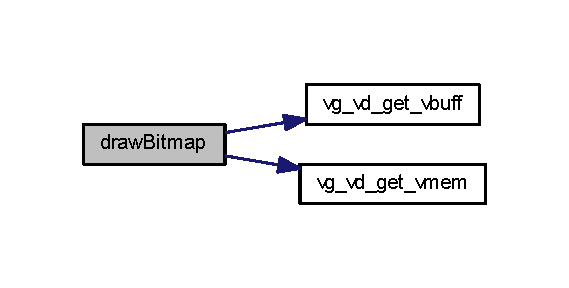
\includegraphics[width=273pt]{group___bitmap_gafe3e5be36ca808fa1383387b7943aa10_cgraph}
\end{center}
\end{figure}
\hypertarget{group___bitmap_ga0dd46e75260201b6cd8211299bf9e703}{}\label{group___bitmap_ga0dd46e75260201b6cd8211299bf9e703} 
\index{Bitmap@{Bitmap}!get\+Image\+Path@{get\+Image\+Path}}
\index{get\+Image\+Path@{get\+Image\+Path}!Bitmap@{Bitmap}}
\subsubsection{\texorpdfstring{get\+Image\+Path()}{getImagePath()}}
{\footnotesize\ttfamily const char$\ast$ get\+Image\+Path (\begin{DoxyParamCaption}\item[{const char $\ast$}]{image }\end{DoxyParamCaption})}

\hypertarget{group___bitmap_ga3506880ffd407c36eb8aaddd2c1606d2}{}\label{group___bitmap_ga3506880ffd407c36eb8aaddd2c1606d2} 
\index{Bitmap@{Bitmap}!load\+Bitmap@{load\+Bitmap}}
\index{load\+Bitmap@{load\+Bitmap}!Bitmap@{Bitmap}}
\subsubsection{\texorpdfstring{load\+Bitmap()}{loadBitmap()}}
{\footnotesize\ttfamily \hyperlink{struct_bitmap}{Bitmap}$\ast$ load\+Bitmap (\begin{DoxyParamCaption}\item[{const char $\ast$}]{filename }\end{DoxyParamCaption})}



Loads a bmp image. 


\begin{DoxyParams}{Parameters}
{\em filename} & Path of the image to load \\
\hline
\end{DoxyParams}
\begin{DoxyReturn}{Returns}
Non N\+U\+LL pointer to the image buffer 
\end{DoxyReturn}

\hypertarget{group__i8254}{}\section{i8254}
\label{group__i8254}\index{i8254@{i8254}}
\subsection*{Macros}
\begin{DoxyCompactItemize}
\item 
\#define \hyperlink{group__i8254_ga30bf84c312af248cb81bb224e09f9ba8}{T\+I\+M\+E\+R0\+\_\+\+I\+RQ}~0
\begin{DoxyCompactList}\small\item\em Timer 0 I\+RQ line. \end{DoxyCompactList}\item 
\#define \hyperlink{group__i8254_gacc9ff9df4a9674a1ce9ba08fc4a4679e}{T\+I\+M\+E\+R\+\_\+0}~0x40
\begin{DoxyCompactList}\small\item\em Timer 0 count register. \end{DoxyCompactList}\item 
\#define \hyperlink{group__i8254_ga282832448fb0281ef53d243c1cd48491}{T\+I\+M\+E\+R\+\_\+\+C\+T\+RL}~0x43
\begin{DoxyCompactList}\small\item\em Control register. \end{DoxyCompactList}\item 
\#define \hyperlink{group__i8254_ga6a4822642d40c248435692324a818010}{T\+I\+M\+E\+R\+\_\+\+S\+E\+L0}~0x00
\begin{DoxyCompactList}\small\item\em Control Word for Timer 0. \end{DoxyCompactList}\item 
\#define \hyperlink{group__i8254_ga4c2eecbfb96744a9c2af71dba75ecb18}{T\+I\+M\+E\+R\+\_\+\+R\+B\+\_\+\+C\+MD}~(\hyperlink{tools_8h_a3a8ea58898cb58fc96013383d39f482c}{B\+IT}(7)$\vert$\hyperlink{tools_8h_a3a8ea58898cb58fc96013383d39f482c}{B\+IT}(6))
\begin{DoxyCompactList}\small\item\em Read Back Command. \end{DoxyCompactList}\item 
\#define \hyperlink{group__i8254_gaa8b3f7a4eeaccbeb4e42a2ca6a9d0cd8}{T\+M0\+\_\+\+I\+R\+Q\+S\+ET}~0
\begin{DoxyCompactList}\small\item\em Timer 0 irq\+\_\+set for bitmask. \end{DoxyCompactList}\item 
\#define \hyperlink{group__i8254_ga1a522aa19bcb695a9df30032a893bee3}{D\+E\+L\+A\+Y\+\_\+\+US}~20000
\end{DoxyCompactItemize}


\subsection{Detailed Description}
Constants for programming the i8254 Timer. 

\subsection{Macro Definition Documentation}
\hypertarget{group__i8254_ga1a522aa19bcb695a9df30032a893bee3}{}\label{group__i8254_ga1a522aa19bcb695a9df30032a893bee3} 
\index{i8254@{i8254}!D\+E\+L\+A\+Y\+\_\+\+US@{D\+E\+L\+A\+Y\+\_\+\+US}}
\index{D\+E\+L\+A\+Y\+\_\+\+US@{D\+E\+L\+A\+Y\+\_\+\+US}!i8254@{i8254}}
\subsubsection{\texorpdfstring{D\+E\+L\+A\+Y\+\_\+\+US}{DELAY\_US}}
{\footnotesize\ttfamily \#define D\+E\+L\+A\+Y\+\_\+\+US~20000}

\hypertarget{group__i8254_ga30bf84c312af248cb81bb224e09f9ba8}{}\label{group__i8254_ga30bf84c312af248cb81bb224e09f9ba8} 
\index{i8254@{i8254}!T\+I\+M\+E\+R0\+\_\+\+I\+RQ@{T\+I\+M\+E\+R0\+\_\+\+I\+RQ}}
\index{T\+I\+M\+E\+R0\+\_\+\+I\+RQ@{T\+I\+M\+E\+R0\+\_\+\+I\+RQ}!i8254@{i8254}}
\subsubsection{\texorpdfstring{T\+I\+M\+E\+R0\+\_\+\+I\+RQ}{TIMER0\_IRQ}}
{\footnotesize\ttfamily \#define T\+I\+M\+E\+R0\+\_\+\+I\+RQ~0}



Timer 0 I\+RQ line. 

\hypertarget{group__i8254_gacc9ff9df4a9674a1ce9ba08fc4a4679e}{}\label{group__i8254_gacc9ff9df4a9674a1ce9ba08fc4a4679e} 
\index{i8254@{i8254}!T\+I\+M\+E\+R\+\_\+0@{T\+I\+M\+E\+R\+\_\+0}}
\index{T\+I\+M\+E\+R\+\_\+0@{T\+I\+M\+E\+R\+\_\+0}!i8254@{i8254}}
\subsubsection{\texorpdfstring{T\+I\+M\+E\+R\+\_\+0}{TIMER\_0}}
{\footnotesize\ttfamily \#define T\+I\+M\+E\+R\+\_\+0~0x40}



Timer 0 count register. 

\hypertarget{group__i8254_ga282832448fb0281ef53d243c1cd48491}{}\label{group__i8254_ga282832448fb0281ef53d243c1cd48491} 
\index{i8254@{i8254}!T\+I\+M\+E\+R\+\_\+\+C\+T\+RL@{T\+I\+M\+E\+R\+\_\+\+C\+T\+RL}}
\index{T\+I\+M\+E\+R\+\_\+\+C\+T\+RL@{T\+I\+M\+E\+R\+\_\+\+C\+T\+RL}!i8254@{i8254}}
\subsubsection{\texorpdfstring{T\+I\+M\+E\+R\+\_\+\+C\+T\+RL}{TIMER\_CTRL}}
{\footnotesize\ttfamily \#define T\+I\+M\+E\+R\+\_\+\+C\+T\+RL~0x43}



Control register. 

\hypertarget{group__i8254_ga4c2eecbfb96744a9c2af71dba75ecb18}{}\label{group__i8254_ga4c2eecbfb96744a9c2af71dba75ecb18} 
\index{i8254@{i8254}!T\+I\+M\+E\+R\+\_\+\+R\+B\+\_\+\+C\+MD@{T\+I\+M\+E\+R\+\_\+\+R\+B\+\_\+\+C\+MD}}
\index{T\+I\+M\+E\+R\+\_\+\+R\+B\+\_\+\+C\+MD@{T\+I\+M\+E\+R\+\_\+\+R\+B\+\_\+\+C\+MD}!i8254@{i8254}}
\subsubsection{\texorpdfstring{T\+I\+M\+E\+R\+\_\+\+R\+B\+\_\+\+C\+MD}{TIMER\_RB\_CMD}}
{\footnotesize\ttfamily \#define T\+I\+M\+E\+R\+\_\+\+R\+B\+\_\+\+C\+MD~(\hyperlink{tools_8h_a3a8ea58898cb58fc96013383d39f482c}{B\+IT}(7)$\vert$\hyperlink{tools_8h_a3a8ea58898cb58fc96013383d39f482c}{B\+IT}(6))}



Read Back Command. 

\hypertarget{group__i8254_ga6a4822642d40c248435692324a818010}{}\label{group__i8254_ga6a4822642d40c248435692324a818010} 
\index{i8254@{i8254}!T\+I\+M\+E\+R\+\_\+\+S\+E\+L0@{T\+I\+M\+E\+R\+\_\+\+S\+E\+L0}}
\index{T\+I\+M\+E\+R\+\_\+\+S\+E\+L0@{T\+I\+M\+E\+R\+\_\+\+S\+E\+L0}!i8254@{i8254}}
\subsubsection{\texorpdfstring{T\+I\+M\+E\+R\+\_\+\+S\+E\+L0}{TIMER\_SEL0}}
{\footnotesize\ttfamily \#define T\+I\+M\+E\+R\+\_\+\+S\+E\+L0~0x00}



Control Word for Timer 0. 

\hypertarget{group__i8254_gaa8b3f7a4eeaccbeb4e42a2ca6a9d0cd8}{}\label{group__i8254_gaa8b3f7a4eeaccbeb4e42a2ca6a9d0cd8} 
\index{i8254@{i8254}!T\+M0\+\_\+\+I\+R\+Q\+S\+ET@{T\+M0\+\_\+\+I\+R\+Q\+S\+ET}}
\index{T\+M0\+\_\+\+I\+R\+Q\+S\+ET@{T\+M0\+\_\+\+I\+R\+Q\+S\+ET}!i8254@{i8254}}
\subsubsection{\texorpdfstring{T\+M0\+\_\+\+I\+R\+Q\+S\+ET}{TM0\_IRQSET}}
{\footnotesize\ttfamily \#define T\+M0\+\_\+\+I\+R\+Q\+S\+ET~0}



Timer 0 irq\+\_\+set for bitmask. 


\hypertarget{group__i8042}{}\section{i8042}
\label{group__i8042}\index{i8042@{i8042}}
\subsection*{Macros}
\begin{DoxyCompactItemize}
\item 
\#define \hyperlink{group__i8042_gae36fc325bc821e866e90d0e66f9cc168}{K\+B\+\_\+\+I\+RQ}~1
\item 
\#define \hyperlink{group__i8042_ga2d17911b50c0aeebb2e3325c5b36d4f2}{K\+E\+Y\+B\+O\+A\+R\+D\+\_\+\+I\+RQ}~1
\item 
\#define \hyperlink{group__i8042_ga923231d2e45aaea2dbab3532b06c2311}{S\+T\+A\+T\+U\+S\+\_\+\+P\+O\+RT}~0x64
\begin{DoxyCompactList}\small\item\em Status Port register. \end{DoxyCompactList}\item 
\#define \hyperlink{group__i8042_gaeff3162e464a9081f73e3765f199d7c1}{K\+B\+D\+\_\+\+O\+U\+T\+\_\+\+B\+UF}~0x60
\begin{DoxyCompactList}\small\item\em Output Buffer register. \end{DoxyCompactList}\item 
\#define \hyperlink{group__i8042_gae1f561b740c8aed366ab0f6618e391f3}{K\+B\+D\+\_\+\+I\+N\+P\+T\+\_\+\+B\+UF}~0x64
\begin{DoxyCompactList}\small\item\em Input Buffer register. \end{DoxyCompactList}\item 
\#define \hyperlink{group__i8042_ga45967c9e25447ba853cf6fb4ac545fe6}{O\+BF}~\hyperlink{tools_8h_a3a8ea58898cb58fc96013383d39f482c}{B\+IT}(0)
\begin{DoxyCompactList}\small\item\em Control Word for Output Buffer Full. \end{DoxyCompactList}\item 
\#define \hyperlink{group__i8042_ga3c48b10907056351582baf9f6478598e}{I\+BF}~\hyperlink{tools_8h_a3a8ea58898cb58fc96013383d39f482c}{B\+IT}(1)
\begin{DoxyCompactList}\small\item\em Control Word for Input Buffer Full. \end{DoxyCompactList}\item 
\#define \hyperlink{group__i8042_gab427e6926fcc47eb1c02c1f78162b6f6}{T\+W\+O\+\_\+\+B\+Y\+T\+ES}~0x\+E0
\begin{DoxyCompactList}\small\item\em Control Word for 2 bytes scancodes. \end{DoxyCompactList}\item 
\#define \hyperlink{group__i8042_ga307ab71673e26ec42b28a3bca05d4cb5}{P\+A\+R\+\_\+\+E\+RR}~\hyperlink{tools_8h_a3a8ea58898cb58fc96013383d39f482c}{B\+IT}(7)
\item 
\#define \hyperlink{group__i8042_gad16f61e2bf70f6c7685e826224ed177f}{T\+O\+\_\+\+E\+RR}~\hyperlink{tools_8h_a3a8ea58898cb58fc96013383d39f482c}{B\+IT}(6)
\end{DoxyCompactItemize}


\subsection{Detailed Description}
Constants for programming the i8042 K\+BC. 

\subsection{Macro Definition Documentation}
\hypertarget{group__i8042_ga3c48b10907056351582baf9f6478598e}{}\label{group__i8042_ga3c48b10907056351582baf9f6478598e} 
\index{i8042@{i8042}!I\+BF@{I\+BF}}
\index{I\+BF@{I\+BF}!i8042@{i8042}}
\subsubsection{\texorpdfstring{I\+BF}{IBF}}
{\footnotesize\ttfamily \#define I\+BF~\hyperlink{tools_8h_a3a8ea58898cb58fc96013383d39f482c}{B\+IT}(1)}



Control Word for Input Buffer Full. 

\hypertarget{group__i8042_gae36fc325bc821e866e90d0e66f9cc168}{}\label{group__i8042_gae36fc325bc821e866e90d0e66f9cc168} 
\index{i8042@{i8042}!K\+B\+\_\+\+I\+RQ@{K\+B\+\_\+\+I\+RQ}}
\index{K\+B\+\_\+\+I\+RQ@{K\+B\+\_\+\+I\+RQ}!i8042@{i8042}}
\subsubsection{\texorpdfstring{K\+B\+\_\+\+I\+RQ}{KB\_IRQ}}
{\footnotesize\ttfamily \#define K\+B\+\_\+\+I\+RQ~1}

\hypertarget{group__i8042_gae1f561b740c8aed366ab0f6618e391f3}{}\label{group__i8042_gae1f561b740c8aed366ab0f6618e391f3} 
\index{i8042@{i8042}!K\+B\+D\+\_\+\+I\+N\+P\+T\+\_\+\+B\+UF@{K\+B\+D\+\_\+\+I\+N\+P\+T\+\_\+\+B\+UF}}
\index{K\+B\+D\+\_\+\+I\+N\+P\+T\+\_\+\+B\+UF@{K\+B\+D\+\_\+\+I\+N\+P\+T\+\_\+\+B\+UF}!i8042@{i8042}}
\subsubsection{\texorpdfstring{K\+B\+D\+\_\+\+I\+N\+P\+T\+\_\+\+B\+UF}{KBD\_INPT\_BUF}}
{\footnotesize\ttfamily \#define K\+B\+D\+\_\+\+I\+N\+P\+T\+\_\+\+B\+UF~0x64}



Input Buffer register. 

\hypertarget{group__i8042_gaeff3162e464a9081f73e3765f199d7c1}{}\label{group__i8042_gaeff3162e464a9081f73e3765f199d7c1} 
\index{i8042@{i8042}!K\+B\+D\+\_\+\+O\+U\+T\+\_\+\+B\+UF@{K\+B\+D\+\_\+\+O\+U\+T\+\_\+\+B\+UF}}
\index{K\+B\+D\+\_\+\+O\+U\+T\+\_\+\+B\+UF@{K\+B\+D\+\_\+\+O\+U\+T\+\_\+\+B\+UF}!i8042@{i8042}}
\subsubsection{\texorpdfstring{K\+B\+D\+\_\+\+O\+U\+T\+\_\+\+B\+UF}{KBD\_OUT\_BUF}}
{\footnotesize\ttfamily \#define K\+B\+D\+\_\+\+O\+U\+T\+\_\+\+B\+UF~0x60}



Output Buffer register. 

\hypertarget{group__i8042_ga2d17911b50c0aeebb2e3325c5b36d4f2}{}\label{group__i8042_ga2d17911b50c0aeebb2e3325c5b36d4f2} 
\index{i8042@{i8042}!K\+E\+Y\+B\+O\+A\+R\+D\+\_\+\+I\+RQ@{K\+E\+Y\+B\+O\+A\+R\+D\+\_\+\+I\+RQ}}
\index{K\+E\+Y\+B\+O\+A\+R\+D\+\_\+\+I\+RQ@{K\+E\+Y\+B\+O\+A\+R\+D\+\_\+\+I\+RQ}!i8042@{i8042}}
\subsubsection{\texorpdfstring{K\+E\+Y\+B\+O\+A\+R\+D\+\_\+\+I\+RQ}{KEYBOARD\_IRQ}}
{\footnotesize\ttfamily \#define K\+E\+Y\+B\+O\+A\+R\+D\+\_\+\+I\+RQ~1}

\hypertarget{group__i8042_ga45967c9e25447ba853cf6fb4ac545fe6}{}\label{group__i8042_ga45967c9e25447ba853cf6fb4ac545fe6} 
\index{i8042@{i8042}!O\+BF@{O\+BF}}
\index{O\+BF@{O\+BF}!i8042@{i8042}}
\subsubsection{\texorpdfstring{O\+BF}{OBF}}
{\footnotesize\ttfamily \#define O\+BF~\hyperlink{tools_8h_a3a8ea58898cb58fc96013383d39f482c}{B\+IT}(0)}



Control Word for Output Buffer Full. 

\hypertarget{group__i8042_ga307ab71673e26ec42b28a3bca05d4cb5}{}\label{group__i8042_ga307ab71673e26ec42b28a3bca05d4cb5} 
\index{i8042@{i8042}!P\+A\+R\+\_\+\+E\+RR@{P\+A\+R\+\_\+\+E\+RR}}
\index{P\+A\+R\+\_\+\+E\+RR@{P\+A\+R\+\_\+\+E\+RR}!i8042@{i8042}}
\subsubsection{\texorpdfstring{P\+A\+R\+\_\+\+E\+RR}{PAR\_ERR}}
{\footnotesize\ttfamily \#define P\+A\+R\+\_\+\+E\+RR~\hyperlink{tools_8h_a3a8ea58898cb58fc96013383d39f482c}{B\+IT}(7)}

\hypertarget{group__i8042_ga923231d2e45aaea2dbab3532b06c2311}{}\label{group__i8042_ga923231d2e45aaea2dbab3532b06c2311} 
\index{i8042@{i8042}!S\+T\+A\+T\+U\+S\+\_\+\+P\+O\+RT@{S\+T\+A\+T\+U\+S\+\_\+\+P\+O\+RT}}
\index{S\+T\+A\+T\+U\+S\+\_\+\+P\+O\+RT@{S\+T\+A\+T\+U\+S\+\_\+\+P\+O\+RT}!i8042@{i8042}}
\subsubsection{\texorpdfstring{S\+T\+A\+T\+U\+S\+\_\+\+P\+O\+RT}{STATUS\_PORT}}
{\footnotesize\ttfamily \#define S\+T\+A\+T\+U\+S\+\_\+\+P\+O\+RT~0x64}



Status Port register. 

\hypertarget{group__i8042_gad16f61e2bf70f6c7685e826224ed177f}{}\label{group__i8042_gad16f61e2bf70f6c7685e826224ed177f} 
\index{i8042@{i8042}!T\+O\+\_\+\+E\+RR@{T\+O\+\_\+\+E\+RR}}
\index{T\+O\+\_\+\+E\+RR@{T\+O\+\_\+\+E\+RR}!i8042@{i8042}}
\subsubsection{\texorpdfstring{T\+O\+\_\+\+E\+RR}{TO\_ERR}}
{\footnotesize\ttfamily \#define T\+O\+\_\+\+E\+RR~\hyperlink{tools_8h_a3a8ea58898cb58fc96013383d39f482c}{B\+IT}(6)}

\hypertarget{group__i8042_gab427e6926fcc47eb1c02c1f78162b6f6}{}\label{group__i8042_gab427e6926fcc47eb1c02c1f78162b6f6} 
\index{i8042@{i8042}!T\+W\+O\+\_\+\+B\+Y\+T\+ES@{T\+W\+O\+\_\+\+B\+Y\+T\+ES}}
\index{T\+W\+O\+\_\+\+B\+Y\+T\+ES@{T\+W\+O\+\_\+\+B\+Y\+T\+ES}!i8042@{i8042}}
\subsubsection{\texorpdfstring{T\+W\+O\+\_\+\+B\+Y\+T\+ES}{TWO\_BYTES}}
{\footnotesize\ttfamily \#define T\+W\+O\+\_\+\+B\+Y\+T\+ES~0x\+E0}



Control Word for 2 bytes scancodes. 


\hypertarget{group__mouse}{}\section{mouse}
\label{group__mouse}\index{mouse@{mouse}}
\subsection*{Macros}
\begin{DoxyCompactItemize}
\item 
\#define \hyperlink{group__mouse_gaf5b75ec709ee94625a79692c87cc7b7a}{M\+O\+U\+S\+E\+\_\+\+S\+E\+ND}~0x\+D4
\item 
\#define \hyperlink{group__mouse_ga7c88f18c3c70a4afefba1a8f772c7036}{M\+O\+U\+S\+E\+\_\+\+E\+NB}~0x\+F4
\item 
\#define \hyperlink{group__mouse_ga199b8aec1af091ef16f1483d4aa4b345}{M\+O\+U\+S\+E\+\_\+\+C\+O\+NF}~0x\+E9
\item 
\#define \hyperlink{group__mouse_ga0349a2901e942eb948442081d0aedc96}{K\+B\+\_\+\+A\+CK}~0x\+FA
\item 
\#define \hyperlink{group__mouse_ga6d57c7927a10f638c83046b52c8caac9}{K\+B\+C\+\_\+\+C\+M\+D\+\_\+\+R\+EG}~0x64
\item 
\#define \hyperlink{group__mouse_ga95745d05db38ca00871939ef479aeb56}{K\+B\+D\+\_\+\+D\+A\+T\+A\+\_\+\+B\+UF}~0x60
\item 
\#define \hyperlink{group__mouse_ga85964cb90343bb1a029b1d1b4229f910}{M\+O\+U\+S\+E\+\_\+\+I\+RQ}~12
\item 
\#define \hyperlink{group__mouse_ga0e16a37e9b19ac48591b3899fc7580ea}{G\+R\+\_\+\+M\+O\+DE}~0x11A
\item 
\#define \hyperlink{group__mouse_ga327c2a8d523460fa45ca05492a003d56}{H\+R\+ES}~1280
\item 
\#define \hyperlink{group__mouse_gacf2cfe6990fa35811b2a0b2f4b77bbdb}{V\+R\+ES}~1024
\item 
\#define \hyperlink{group__mouse_gaee3d3431c33559daa9472d32dbaa76cc}{X\+L\+L\+I\+M\+IT}~50
\item 
\#define \hyperlink{group__mouse_gaccc38829dd9a253af163a2e05124d239}{X\+R\+L\+I\+M\+IT}~1250
\item 
\#define \hyperlink{group__mouse_ga7afa9a9c3f789856869ae1a766cc917f}{Y\+U\+L\+I\+M\+IT}~200
\item 
\#define \hyperlink{group__mouse_gaec42b751ff3806b4f7102f7564fdf34d}{Y\+D\+L\+I\+M\+IT}~1000
\item 
\#define \hyperlink{group__mouse_ga4a627ba1f66cbd6c5de585d5002ebe96}{M\+E\+N\+U1U}~347
\item 
\#define \hyperlink{group__mouse_gabc4d39c53c1b122b66301e6d91fec329}{M\+E\+N\+U1D}~435
\item 
\#define \hyperlink{group__mouse_gaf46df8ae7d292764e0bd733b5a69fa97}{M\+E\+N\+U1L}~221
\item 
\#define \hyperlink{group__mouse_ga280f604342f10e7da8eb79e5364f134e}{M\+E\+N\+U1R}~578
\item 
\#define \hyperlink{group__mouse_gad344b0e0080be13940f676b3fb921604}{M\+E\+N\+U2U}~347
\item 
\#define \hyperlink{group__mouse_ga5f1d419164811a353a3fb91ab934b008}{M\+E\+N\+U2D}~435
\item 
\#define \hyperlink{group__mouse_gaf9c31d922032006354f0f94d0dbfba86}{M\+E\+N\+U2L}~715
\item 
\#define \hyperlink{group__mouse_ga9ba96b159609610c99e1e56ae532ce2e}{M\+E\+N\+U2R}~1071
\item 
\#define \hyperlink{group__mouse_ga58d0568b55739b936c55a4cd70642273}{M\+E\+N\+U3U}~526
\item 
\#define \hyperlink{group__mouse_ga1bf711f126b31c1e93c4273139dda3d5}{M\+E\+N\+U3D}~614
\item 
\#define \hyperlink{group__mouse_ga261b94752f05faaea72b95f89fb4eaae}{M\+E\+N\+U3L}~221
\item 
\#define \hyperlink{group__mouse_ga4b14d3a27693996fda99359c830d3d0f}{M\+E\+N\+U3R}~578
\item 
\#define \hyperlink{group__mouse_gaaa91c726154bcb919ad804280ef7b402}{M\+E\+N\+U4U}~526
\item 
\#define \hyperlink{group__mouse_ga49904fe1a8177385da2f91915bd5e123}{M\+E\+N\+U4D}~614
\item 
\#define \hyperlink{group__mouse_ga455cfaa20c07781a8036731bd000b7f4}{M\+E\+N\+U4L}~715
\item 
\#define \hyperlink{group__mouse_ga1234a94f05b8102de0c93698aaf08085}{M\+E\+N\+U4R}~1071
\end{DoxyCompactItemize}


\subsection{Detailed Description}
Constants for programming the mouse. 

\subsection{Macro Definition Documentation}
\hypertarget{group__mouse_ga0e16a37e9b19ac48591b3899fc7580ea}{}\label{group__mouse_ga0e16a37e9b19ac48591b3899fc7580ea} 
\index{mouse@{mouse}!G\+R\+\_\+\+M\+O\+DE@{G\+R\+\_\+\+M\+O\+DE}}
\index{G\+R\+\_\+\+M\+O\+DE@{G\+R\+\_\+\+M\+O\+DE}!mouse@{mouse}}
\subsubsection{\texorpdfstring{G\+R\+\_\+\+M\+O\+DE}{GR\_MODE}}
{\footnotesize\ttfamily \#define G\+R\+\_\+\+M\+O\+DE~0x11A}

\hypertarget{group__mouse_ga327c2a8d523460fa45ca05492a003d56}{}\label{group__mouse_ga327c2a8d523460fa45ca05492a003d56} 
\index{mouse@{mouse}!H\+R\+ES@{H\+R\+ES}}
\index{H\+R\+ES@{H\+R\+ES}!mouse@{mouse}}
\subsubsection{\texorpdfstring{H\+R\+ES}{HRES}}
{\footnotesize\ttfamily \#define H\+R\+ES~1280}

\hypertarget{group__mouse_ga0349a2901e942eb948442081d0aedc96}{}\label{group__mouse_ga0349a2901e942eb948442081d0aedc96} 
\index{mouse@{mouse}!K\+B\+\_\+\+A\+CK@{K\+B\+\_\+\+A\+CK}}
\index{K\+B\+\_\+\+A\+CK@{K\+B\+\_\+\+A\+CK}!mouse@{mouse}}
\subsubsection{\texorpdfstring{K\+B\+\_\+\+A\+CK}{KB\_ACK}}
{\footnotesize\ttfamily \#define K\+B\+\_\+\+A\+CK~0x\+FA}

\hypertarget{group__mouse_ga6d57c7927a10f638c83046b52c8caac9}{}\label{group__mouse_ga6d57c7927a10f638c83046b52c8caac9} 
\index{mouse@{mouse}!K\+B\+C\+\_\+\+C\+M\+D\+\_\+\+R\+EG@{K\+B\+C\+\_\+\+C\+M\+D\+\_\+\+R\+EG}}
\index{K\+B\+C\+\_\+\+C\+M\+D\+\_\+\+R\+EG@{K\+B\+C\+\_\+\+C\+M\+D\+\_\+\+R\+EG}!mouse@{mouse}}
\subsubsection{\texorpdfstring{K\+B\+C\+\_\+\+C\+M\+D\+\_\+\+R\+EG}{KBC\_CMD\_REG}}
{\footnotesize\ttfamily \#define K\+B\+C\+\_\+\+C\+M\+D\+\_\+\+R\+EG~0x64}

\hypertarget{group__mouse_ga95745d05db38ca00871939ef479aeb56}{}\label{group__mouse_ga95745d05db38ca00871939ef479aeb56} 
\index{mouse@{mouse}!K\+B\+D\+\_\+\+D\+A\+T\+A\+\_\+\+B\+UF@{K\+B\+D\+\_\+\+D\+A\+T\+A\+\_\+\+B\+UF}}
\index{K\+B\+D\+\_\+\+D\+A\+T\+A\+\_\+\+B\+UF@{K\+B\+D\+\_\+\+D\+A\+T\+A\+\_\+\+B\+UF}!mouse@{mouse}}
\subsubsection{\texorpdfstring{K\+B\+D\+\_\+\+D\+A\+T\+A\+\_\+\+B\+UF}{KBD\_DATA\_BUF}}
{\footnotesize\ttfamily \#define K\+B\+D\+\_\+\+D\+A\+T\+A\+\_\+\+B\+UF~0x60}

\hypertarget{group__mouse_gabc4d39c53c1b122b66301e6d91fec329}{}\label{group__mouse_gabc4d39c53c1b122b66301e6d91fec329} 
\index{mouse@{mouse}!M\+E\+N\+U1D@{M\+E\+N\+U1D}}
\index{M\+E\+N\+U1D@{M\+E\+N\+U1D}!mouse@{mouse}}
\subsubsection{\texorpdfstring{M\+E\+N\+U1D}{MENU1D}}
{\footnotesize\ttfamily \#define M\+E\+N\+U1D~435}

\hypertarget{group__mouse_gaf46df8ae7d292764e0bd733b5a69fa97}{}\label{group__mouse_gaf46df8ae7d292764e0bd733b5a69fa97} 
\index{mouse@{mouse}!M\+E\+N\+U1L@{M\+E\+N\+U1L}}
\index{M\+E\+N\+U1L@{M\+E\+N\+U1L}!mouse@{mouse}}
\subsubsection{\texorpdfstring{M\+E\+N\+U1L}{MENU1L}}
{\footnotesize\ttfamily \#define M\+E\+N\+U1L~221}

\hypertarget{group__mouse_ga280f604342f10e7da8eb79e5364f134e}{}\label{group__mouse_ga280f604342f10e7da8eb79e5364f134e} 
\index{mouse@{mouse}!M\+E\+N\+U1R@{M\+E\+N\+U1R}}
\index{M\+E\+N\+U1R@{M\+E\+N\+U1R}!mouse@{mouse}}
\subsubsection{\texorpdfstring{M\+E\+N\+U1R}{MENU1R}}
{\footnotesize\ttfamily \#define M\+E\+N\+U1R~578}

\hypertarget{group__mouse_ga4a627ba1f66cbd6c5de585d5002ebe96}{}\label{group__mouse_ga4a627ba1f66cbd6c5de585d5002ebe96} 
\index{mouse@{mouse}!M\+E\+N\+U1U@{M\+E\+N\+U1U}}
\index{M\+E\+N\+U1U@{M\+E\+N\+U1U}!mouse@{mouse}}
\subsubsection{\texorpdfstring{M\+E\+N\+U1U}{MENU1U}}
{\footnotesize\ttfamily \#define M\+E\+N\+U1U~347}

\hypertarget{group__mouse_ga5f1d419164811a353a3fb91ab934b008}{}\label{group__mouse_ga5f1d419164811a353a3fb91ab934b008} 
\index{mouse@{mouse}!M\+E\+N\+U2D@{M\+E\+N\+U2D}}
\index{M\+E\+N\+U2D@{M\+E\+N\+U2D}!mouse@{mouse}}
\subsubsection{\texorpdfstring{M\+E\+N\+U2D}{MENU2D}}
{\footnotesize\ttfamily \#define M\+E\+N\+U2D~435}

\hypertarget{group__mouse_gaf9c31d922032006354f0f94d0dbfba86}{}\label{group__mouse_gaf9c31d922032006354f0f94d0dbfba86} 
\index{mouse@{mouse}!M\+E\+N\+U2L@{M\+E\+N\+U2L}}
\index{M\+E\+N\+U2L@{M\+E\+N\+U2L}!mouse@{mouse}}
\subsubsection{\texorpdfstring{M\+E\+N\+U2L}{MENU2L}}
{\footnotesize\ttfamily \#define M\+E\+N\+U2L~715}

\hypertarget{group__mouse_ga9ba96b159609610c99e1e56ae532ce2e}{}\label{group__mouse_ga9ba96b159609610c99e1e56ae532ce2e} 
\index{mouse@{mouse}!M\+E\+N\+U2R@{M\+E\+N\+U2R}}
\index{M\+E\+N\+U2R@{M\+E\+N\+U2R}!mouse@{mouse}}
\subsubsection{\texorpdfstring{M\+E\+N\+U2R}{MENU2R}}
{\footnotesize\ttfamily \#define M\+E\+N\+U2R~1071}

\hypertarget{group__mouse_gad344b0e0080be13940f676b3fb921604}{}\label{group__mouse_gad344b0e0080be13940f676b3fb921604} 
\index{mouse@{mouse}!M\+E\+N\+U2U@{M\+E\+N\+U2U}}
\index{M\+E\+N\+U2U@{M\+E\+N\+U2U}!mouse@{mouse}}
\subsubsection{\texorpdfstring{M\+E\+N\+U2U}{MENU2U}}
{\footnotesize\ttfamily \#define M\+E\+N\+U2U~347}

\hypertarget{group__mouse_ga1bf711f126b31c1e93c4273139dda3d5}{}\label{group__mouse_ga1bf711f126b31c1e93c4273139dda3d5} 
\index{mouse@{mouse}!M\+E\+N\+U3D@{M\+E\+N\+U3D}}
\index{M\+E\+N\+U3D@{M\+E\+N\+U3D}!mouse@{mouse}}
\subsubsection{\texorpdfstring{M\+E\+N\+U3D}{MENU3D}}
{\footnotesize\ttfamily \#define M\+E\+N\+U3D~614}

\hypertarget{group__mouse_ga261b94752f05faaea72b95f89fb4eaae}{}\label{group__mouse_ga261b94752f05faaea72b95f89fb4eaae} 
\index{mouse@{mouse}!M\+E\+N\+U3L@{M\+E\+N\+U3L}}
\index{M\+E\+N\+U3L@{M\+E\+N\+U3L}!mouse@{mouse}}
\subsubsection{\texorpdfstring{M\+E\+N\+U3L}{MENU3L}}
{\footnotesize\ttfamily \#define M\+E\+N\+U3L~221}

\hypertarget{group__mouse_ga4b14d3a27693996fda99359c830d3d0f}{}\label{group__mouse_ga4b14d3a27693996fda99359c830d3d0f} 
\index{mouse@{mouse}!M\+E\+N\+U3R@{M\+E\+N\+U3R}}
\index{M\+E\+N\+U3R@{M\+E\+N\+U3R}!mouse@{mouse}}
\subsubsection{\texorpdfstring{M\+E\+N\+U3R}{MENU3R}}
{\footnotesize\ttfamily \#define M\+E\+N\+U3R~578}

\hypertarget{group__mouse_ga58d0568b55739b936c55a4cd70642273}{}\label{group__mouse_ga58d0568b55739b936c55a4cd70642273} 
\index{mouse@{mouse}!M\+E\+N\+U3U@{M\+E\+N\+U3U}}
\index{M\+E\+N\+U3U@{M\+E\+N\+U3U}!mouse@{mouse}}
\subsubsection{\texorpdfstring{M\+E\+N\+U3U}{MENU3U}}
{\footnotesize\ttfamily \#define M\+E\+N\+U3U~526}

\hypertarget{group__mouse_ga49904fe1a8177385da2f91915bd5e123}{}\label{group__mouse_ga49904fe1a8177385da2f91915bd5e123} 
\index{mouse@{mouse}!M\+E\+N\+U4D@{M\+E\+N\+U4D}}
\index{M\+E\+N\+U4D@{M\+E\+N\+U4D}!mouse@{mouse}}
\subsubsection{\texorpdfstring{M\+E\+N\+U4D}{MENU4D}}
{\footnotesize\ttfamily \#define M\+E\+N\+U4D~614}

\hypertarget{group__mouse_ga455cfaa20c07781a8036731bd000b7f4}{}\label{group__mouse_ga455cfaa20c07781a8036731bd000b7f4} 
\index{mouse@{mouse}!M\+E\+N\+U4L@{M\+E\+N\+U4L}}
\index{M\+E\+N\+U4L@{M\+E\+N\+U4L}!mouse@{mouse}}
\subsubsection{\texorpdfstring{M\+E\+N\+U4L}{MENU4L}}
{\footnotesize\ttfamily \#define M\+E\+N\+U4L~715}

\hypertarget{group__mouse_ga1234a94f05b8102de0c93698aaf08085}{}\label{group__mouse_ga1234a94f05b8102de0c93698aaf08085} 
\index{mouse@{mouse}!M\+E\+N\+U4R@{M\+E\+N\+U4R}}
\index{M\+E\+N\+U4R@{M\+E\+N\+U4R}!mouse@{mouse}}
\subsubsection{\texorpdfstring{M\+E\+N\+U4R}{MENU4R}}
{\footnotesize\ttfamily \#define M\+E\+N\+U4R~1071}

\hypertarget{group__mouse_gaaa91c726154bcb919ad804280ef7b402}{}\label{group__mouse_gaaa91c726154bcb919ad804280ef7b402} 
\index{mouse@{mouse}!M\+E\+N\+U4U@{M\+E\+N\+U4U}}
\index{M\+E\+N\+U4U@{M\+E\+N\+U4U}!mouse@{mouse}}
\subsubsection{\texorpdfstring{M\+E\+N\+U4U}{MENU4U}}
{\footnotesize\ttfamily \#define M\+E\+N\+U4U~526}

\hypertarget{group__mouse_ga199b8aec1af091ef16f1483d4aa4b345}{}\label{group__mouse_ga199b8aec1af091ef16f1483d4aa4b345} 
\index{mouse@{mouse}!M\+O\+U\+S\+E\+\_\+\+C\+O\+NF@{M\+O\+U\+S\+E\+\_\+\+C\+O\+NF}}
\index{M\+O\+U\+S\+E\+\_\+\+C\+O\+NF@{M\+O\+U\+S\+E\+\_\+\+C\+O\+NF}!mouse@{mouse}}
\subsubsection{\texorpdfstring{M\+O\+U\+S\+E\+\_\+\+C\+O\+NF}{MOUSE\_CONF}}
{\footnotesize\ttfamily \#define M\+O\+U\+S\+E\+\_\+\+C\+O\+NF~0x\+E9}

\hypertarget{group__mouse_ga7c88f18c3c70a4afefba1a8f772c7036}{}\label{group__mouse_ga7c88f18c3c70a4afefba1a8f772c7036} 
\index{mouse@{mouse}!M\+O\+U\+S\+E\+\_\+\+E\+NB@{M\+O\+U\+S\+E\+\_\+\+E\+NB}}
\index{M\+O\+U\+S\+E\+\_\+\+E\+NB@{M\+O\+U\+S\+E\+\_\+\+E\+NB}!mouse@{mouse}}
\subsubsection{\texorpdfstring{M\+O\+U\+S\+E\+\_\+\+E\+NB}{MOUSE\_ENB}}
{\footnotesize\ttfamily \#define M\+O\+U\+S\+E\+\_\+\+E\+NB~0x\+F4}

\hypertarget{group__mouse_ga85964cb90343bb1a029b1d1b4229f910}{}\label{group__mouse_ga85964cb90343bb1a029b1d1b4229f910} 
\index{mouse@{mouse}!M\+O\+U\+S\+E\+\_\+\+I\+RQ@{M\+O\+U\+S\+E\+\_\+\+I\+RQ}}
\index{M\+O\+U\+S\+E\+\_\+\+I\+RQ@{M\+O\+U\+S\+E\+\_\+\+I\+RQ}!mouse@{mouse}}
\subsubsection{\texorpdfstring{M\+O\+U\+S\+E\+\_\+\+I\+RQ}{MOUSE\_IRQ}}
{\footnotesize\ttfamily \#define M\+O\+U\+S\+E\+\_\+\+I\+RQ~12}

\hypertarget{group__mouse_gaf5b75ec709ee94625a79692c87cc7b7a}{}\label{group__mouse_gaf5b75ec709ee94625a79692c87cc7b7a} 
\index{mouse@{mouse}!M\+O\+U\+S\+E\+\_\+\+S\+E\+ND@{M\+O\+U\+S\+E\+\_\+\+S\+E\+ND}}
\index{M\+O\+U\+S\+E\+\_\+\+S\+E\+ND@{M\+O\+U\+S\+E\+\_\+\+S\+E\+ND}!mouse@{mouse}}
\subsubsection{\texorpdfstring{M\+O\+U\+S\+E\+\_\+\+S\+E\+ND}{MOUSE\_SEND}}
{\footnotesize\ttfamily \#define M\+O\+U\+S\+E\+\_\+\+S\+E\+ND~0x\+D4}

\hypertarget{group__mouse_gacf2cfe6990fa35811b2a0b2f4b77bbdb}{}\label{group__mouse_gacf2cfe6990fa35811b2a0b2f4b77bbdb} 
\index{mouse@{mouse}!V\+R\+ES@{V\+R\+ES}}
\index{V\+R\+ES@{V\+R\+ES}!mouse@{mouse}}
\subsubsection{\texorpdfstring{V\+R\+ES}{VRES}}
{\footnotesize\ttfamily \#define V\+R\+ES~1024}

\hypertarget{group__mouse_gaee3d3431c33559daa9472d32dbaa76cc}{}\label{group__mouse_gaee3d3431c33559daa9472d32dbaa76cc} 
\index{mouse@{mouse}!X\+L\+L\+I\+M\+IT@{X\+L\+L\+I\+M\+IT}}
\index{X\+L\+L\+I\+M\+IT@{X\+L\+L\+I\+M\+IT}!mouse@{mouse}}
\subsubsection{\texorpdfstring{X\+L\+L\+I\+M\+IT}{XLLIMIT}}
{\footnotesize\ttfamily \#define X\+L\+L\+I\+M\+IT~50}

\hypertarget{group__mouse_gaccc38829dd9a253af163a2e05124d239}{}\label{group__mouse_gaccc38829dd9a253af163a2e05124d239} 
\index{mouse@{mouse}!X\+R\+L\+I\+M\+IT@{X\+R\+L\+I\+M\+IT}}
\index{X\+R\+L\+I\+M\+IT@{X\+R\+L\+I\+M\+IT}!mouse@{mouse}}
\subsubsection{\texorpdfstring{X\+R\+L\+I\+M\+IT}{XRLIMIT}}
{\footnotesize\ttfamily \#define X\+R\+L\+I\+M\+IT~1250}

\hypertarget{group__mouse_gaec42b751ff3806b4f7102f7564fdf34d}{}\label{group__mouse_gaec42b751ff3806b4f7102f7564fdf34d} 
\index{mouse@{mouse}!Y\+D\+L\+I\+M\+IT@{Y\+D\+L\+I\+M\+IT}}
\index{Y\+D\+L\+I\+M\+IT@{Y\+D\+L\+I\+M\+IT}!mouse@{mouse}}
\subsubsection{\texorpdfstring{Y\+D\+L\+I\+M\+IT}{YDLIMIT}}
{\footnotesize\ttfamily \#define Y\+D\+L\+I\+M\+IT~1000}

\hypertarget{group__mouse_ga7afa9a9c3f789856869ae1a766cc917f}{}\label{group__mouse_ga7afa9a9c3f789856869ae1a766cc917f} 
\index{mouse@{mouse}!Y\+U\+L\+I\+M\+IT@{Y\+U\+L\+I\+M\+IT}}
\index{Y\+U\+L\+I\+M\+IT@{Y\+U\+L\+I\+M\+IT}!mouse@{mouse}}
\subsubsection{\texorpdfstring{Y\+U\+L\+I\+M\+IT}{YULIMIT}}
{\footnotesize\ttfamily \#define Y\+U\+L\+I\+M\+IT~200}


\hypertarget{group__colors}{}\section{colors}
\label{group__colors}\index{colors@{colors}}
\subsection*{Macros}
\begin{DoxyCompactItemize}
\item 
\#define \hyperlink{group__colors_gabc93b0adf636edc12e8e9e0489429972}{O\+R\+A\+N\+G\+E1}~\hyperlink{group__colors_ga8ac8469511c64983e8f0a678a14f0e36}{rgb}(223,116,12);
\item 
\#define \hyperlink{group__colors_ga8ac45568d18ed08eb1ff4e9355110f6e}{O\+R\+A\+N\+G\+E2}~\hyperlink{group__colors_ga8ac8469511c64983e8f0a678a14f0e36}{rgb}(255,230,77);
\item 
\#define \hyperlink{group__colors_ga30100d62cd1f80d21430872e1be9c543}{B\+L\+U\+E1}~\hyperlink{group__colors_ga8ac8469511c64983e8f0a678a14f0e36}{rgb}(111,195,223);
\item 
\#define \hyperlink{group__colors_ga741d26513518e80fdef905dc6f209fc8}{B\+L\+U\+E2}~\hyperlink{group__colors_ga8ac8469511c64983e8f0a678a14f0e36}{rgb}(230,255,255);
\item 
\#define \hyperlink{group__colors_ga343686a86fcf4e10a82059b078b1b7d0}{G\+R\+E\+E\+N1}~\hyperlink{group__colors_ga8ac8469511c64983e8f0a678a14f0e36}{rgb}(8,254,20);
\item 
\#define \hyperlink{group__colors_ga0514cf5f3dd5549be9c93c6ec588dbd5}{P\+I\+N\+K1}~\hyperlink{group__colors_ga8ac8469511c64983e8f0a678a14f0e36}{rgb}(255,54,155);
\item 
\#define \hyperlink{group__colors_ga87b537f5fa5c109d3c05c13d6b18f382}{W\+H\+I\+TE}~\hyperlink{group__colors_ga8ac8469511c64983e8f0a678a14f0e36}{rgb}(255,255,255);
\item 
\#define \hyperlink{group__colors_ga7b3b25cba33b07c303f3060fe41887f6}{B\+L\+A\+CK}~\hyperlink{group__colors_ga8ac8469511c64983e8f0a678a14f0e36}{rgb}(0,0,0);
\end{DoxyCompactItemize}
\subsection*{Functions}
\begin{DoxyCompactItemize}
\item 
int \hyperlink{group__colors_ga8ac8469511c64983e8f0a678a14f0e36}{rgb} (unsigned char r, unsigned char g, unsigned char b)
\begin{DoxyCompactList}\small\item\em Calculates a color in R\+BG 5\+:6\+:5. \end{DoxyCompactList}\end{DoxyCompactItemize}


\subsection{Detailed Description}
Colors for painting. 

\subsection{Macro Definition Documentation}
\hypertarget{group__colors_ga7b3b25cba33b07c303f3060fe41887f6}{}\label{group__colors_ga7b3b25cba33b07c303f3060fe41887f6} 
\index{colors@{colors}!B\+L\+A\+CK@{B\+L\+A\+CK}}
\index{B\+L\+A\+CK@{B\+L\+A\+CK}!colors@{colors}}
\subsubsection{\texorpdfstring{B\+L\+A\+CK}{BLACK}}
{\footnotesize\ttfamily \#define B\+L\+A\+CK~\hyperlink{group__colors_ga8ac8469511c64983e8f0a678a14f0e36}{rgb}(0,0,0);}

\hypertarget{group__colors_ga30100d62cd1f80d21430872e1be9c543}{}\label{group__colors_ga30100d62cd1f80d21430872e1be9c543} 
\index{colors@{colors}!B\+L\+U\+E1@{B\+L\+U\+E1}}
\index{B\+L\+U\+E1@{B\+L\+U\+E1}!colors@{colors}}
\subsubsection{\texorpdfstring{B\+L\+U\+E1}{BLUE1}}
{\footnotesize\ttfamily \#define B\+L\+U\+E1~\hyperlink{group__colors_ga8ac8469511c64983e8f0a678a14f0e36}{rgb}(111,195,223);}

\hypertarget{group__colors_ga741d26513518e80fdef905dc6f209fc8}{}\label{group__colors_ga741d26513518e80fdef905dc6f209fc8} 
\index{colors@{colors}!B\+L\+U\+E2@{B\+L\+U\+E2}}
\index{B\+L\+U\+E2@{B\+L\+U\+E2}!colors@{colors}}
\subsubsection{\texorpdfstring{B\+L\+U\+E2}{BLUE2}}
{\footnotesize\ttfamily \#define B\+L\+U\+E2~\hyperlink{group__colors_ga8ac8469511c64983e8f0a678a14f0e36}{rgb}(230,255,255);}

\hypertarget{group__colors_ga343686a86fcf4e10a82059b078b1b7d0}{}\label{group__colors_ga343686a86fcf4e10a82059b078b1b7d0} 
\index{colors@{colors}!G\+R\+E\+E\+N1@{G\+R\+E\+E\+N1}}
\index{G\+R\+E\+E\+N1@{G\+R\+E\+E\+N1}!colors@{colors}}
\subsubsection{\texorpdfstring{G\+R\+E\+E\+N1}{GREEN1}}
{\footnotesize\ttfamily \#define G\+R\+E\+E\+N1~\hyperlink{group__colors_ga8ac8469511c64983e8f0a678a14f0e36}{rgb}(8,254,20);}

\hypertarget{group__colors_gabc93b0adf636edc12e8e9e0489429972}{}\label{group__colors_gabc93b0adf636edc12e8e9e0489429972} 
\index{colors@{colors}!O\+R\+A\+N\+G\+E1@{O\+R\+A\+N\+G\+E1}}
\index{O\+R\+A\+N\+G\+E1@{O\+R\+A\+N\+G\+E1}!colors@{colors}}
\subsubsection{\texorpdfstring{O\+R\+A\+N\+G\+E1}{ORANGE1}}
{\footnotesize\ttfamily \#define O\+R\+A\+N\+G\+E1~\hyperlink{group__colors_ga8ac8469511c64983e8f0a678a14f0e36}{rgb}(223,116,12);}

\hypertarget{group__colors_ga8ac45568d18ed08eb1ff4e9355110f6e}{}\label{group__colors_ga8ac45568d18ed08eb1ff4e9355110f6e} 
\index{colors@{colors}!O\+R\+A\+N\+G\+E2@{O\+R\+A\+N\+G\+E2}}
\index{O\+R\+A\+N\+G\+E2@{O\+R\+A\+N\+G\+E2}!colors@{colors}}
\subsubsection{\texorpdfstring{O\+R\+A\+N\+G\+E2}{ORANGE2}}
{\footnotesize\ttfamily \#define O\+R\+A\+N\+G\+E2~\hyperlink{group__colors_ga8ac8469511c64983e8f0a678a14f0e36}{rgb}(255,230,77);}

\hypertarget{group__colors_ga0514cf5f3dd5549be9c93c6ec588dbd5}{}\label{group__colors_ga0514cf5f3dd5549be9c93c6ec588dbd5} 
\index{colors@{colors}!P\+I\+N\+K1@{P\+I\+N\+K1}}
\index{P\+I\+N\+K1@{P\+I\+N\+K1}!colors@{colors}}
\subsubsection{\texorpdfstring{P\+I\+N\+K1}{PINK1}}
{\footnotesize\ttfamily \#define P\+I\+N\+K1~\hyperlink{group__colors_ga8ac8469511c64983e8f0a678a14f0e36}{rgb}(255,54,155);}

\hypertarget{group__colors_ga87b537f5fa5c109d3c05c13d6b18f382}{}\label{group__colors_ga87b537f5fa5c109d3c05c13d6b18f382} 
\index{colors@{colors}!W\+H\+I\+TE@{W\+H\+I\+TE}}
\index{W\+H\+I\+TE@{W\+H\+I\+TE}!colors@{colors}}
\subsubsection{\texorpdfstring{W\+H\+I\+TE}{WHITE}}
{\footnotesize\ttfamily \#define W\+H\+I\+TE~\hyperlink{group__colors_ga8ac8469511c64983e8f0a678a14f0e36}{rgb}(255,255,255);}



\subsection{Function Documentation}
\hypertarget{group__colors_ga8ac8469511c64983e8f0a678a14f0e36}{}\label{group__colors_ga8ac8469511c64983e8f0a678a14f0e36} 
\index{colors@{colors}!rgb@{rgb}}
\index{rgb@{rgb}!colors@{colors}}
\subsubsection{\texorpdfstring{rgb()}{rgb()}}
{\footnotesize\ttfamily int rgb (\begin{DoxyParamCaption}\item[{unsigned char}]{r,  }\item[{unsigned char}]{g,  }\item[{unsigned char}]{b }\end{DoxyParamCaption})}



Calculates a color in R\+BG 5\+:6\+:5. 

R\+GB function from \href{http://stackoverflow.com/questions/27194568/rgb-color-converting-into-565-format}{\tt http\+://stackoverflow.\+com/questions/27194568/rgb-\/color-\/converting-\/into-\/565-\/format} author\+: PiotrK


\begin{DoxyParams}{Parameters}
{\em r} & Red color value \\
\hline
{\em g} & Green color value \\
\hline
{\em b} & Blue color value \\
\hline
\end{DoxyParams}
\begin{DoxyReturn}{Returns}
Returns the color in R\+GB 5\+:6\+:5 
\end{DoxyReturn}

\hypertarget{group__scancodes}{}\section{scancodes}
\label{group__scancodes}\index{scancodes@{scancodes}}
\subsection*{Macros}
\begin{DoxyCompactItemize}
\item 
\#define \hyperlink{group__scancodes_ga343f44cb034d2d2ff3438b3d45dcde1f}{E\+S\+C\+\_\+\+B\+R\+E\+AK}~0x81
\item 
\#define \hyperlink{group__scancodes_ga168fd0a54619731c76c386a7f1bde2b1}{E\+S\+C\+\_\+\+M\+A\+KE}~0x01
\item 
\#define \hyperlink{group__scancodes_ga95d6e4b61bac77469ecc47b205709af6}{S\+P\+A\+C\+E\+\_\+\+B\+R\+E\+AK}~0x\+B9
\item 
\#define \hyperlink{group__scancodes_ga0f76fe84c649e8cf3a4114d0d9bf085a}{A\+\_\+\+M\+A\+KE}~0x1E
\item 
\#define \hyperlink{group__scancodes_ga05826112c5acf959ee58dcacd8e9d065}{A\+\_\+\+B\+R\+E\+AK}~0x9E
\item 
\#define \hyperlink{group__scancodes_gac822a3953d90207e64b58f480454a8d8}{W\+\_\+\+M\+A\+KE}~0x11
\item 
\#define \hyperlink{group__scancodes_ga32d11f9abffe8bb3df11feef5ca5213d}{W\+\_\+\+B\+R\+E\+AK}~0x91
\item 
\#define \hyperlink{group__scancodes_gac2c2b345d42f2a5b5a028028eb8c5680}{S\+\_\+\+M\+A\+KE}~0x1F
\item 
\#define \hyperlink{group__scancodes_ga85b3c65b8b6c952e08c252e9737b74f9}{S\+\_\+\+B\+R\+E\+AK}~0x9F
\item 
\#define \hyperlink{group__scancodes_ga629b0c93e278a4bf1e1678af58fbea95}{D\+\_\+\+M\+A\+KE}~0x20
\item 
\#define \hyperlink{group__scancodes_gad2db9242348c43c781cc14746060470b}{D\+\_\+\+B\+R\+E\+AK}~0x\+A0
\item 
\#define \hyperlink{group__scancodes_ga4c8f4d4420f9ec7ef30de25264efa68a}{U\+A\+R\+R\+O\+W\+\_\+\+M\+A\+KE}~0x\+E048
\item 
\#define \hyperlink{group__scancodes_ga9ab3dee73aef06dca9ef9b37b818acb2}{U\+A\+R\+R\+O\+W\+\_\+\+B\+R\+E\+AK}~0x\+E0\+C8
\item 
\#define \hyperlink{group__scancodes_gad9509ca6995b9d5ca117d0ea8004cfef}{L\+A\+R\+R\+O\+W\+\_\+\+M\+A\+KE}~0x\+E04B
\item 
\#define \hyperlink{group__scancodes_ga335ac9047c7a6d0c8631014766f96484}{L\+A\+R\+R\+O\+W\+\_\+\+B\+R\+E\+AK}~0x\+E0\+CB
\item 
\#define \hyperlink{group__scancodes_ga5e0594973062eb7d381ee43ff19a0369}{D\+A\+R\+R\+O\+W\+\_\+\+M\+A\+KE}~0x\+E050
\item 
\#define \hyperlink{group__scancodes_ga02742462a869b87ad2a34d8bc6a3fe58}{D\+A\+R\+R\+O\+W\+\_\+\+B\+R\+E\+AK}~0x\+E0\+D0
\item 
\#define \hyperlink{group__scancodes_ga365f3fec5881bea630c70f2c1098263f}{R\+A\+R\+R\+O\+W\+\_\+\+M\+A\+KE}~0x\+E04D
\item 
\#define \hyperlink{group__scancodes_ga9dd5fb482207f2c4f76696b443f76020}{R\+A\+R\+R\+O\+W\+\_\+\+B\+R\+E\+AK}~0x\+E0\+CD
\item 
\#define \hyperlink{group__scancodes_gaa7a13a11c6b4a4b22cc8c2dd5cca7a95}{B\+\_\+\+M\+A\+KE}~0x30
\item 
\#define \hyperlink{group__scancodes_ga357a1debdc4027db65b315366e9019dd}{M\+\_\+\+M\+A\+KE}~0x32
\item 
\#define \hyperlink{group__scancodes_ga124c06c60ba6b840260900c1fa975163}{I\+\_\+\+M\+A\+KE}~0x17
\item 
\#define \hyperlink{group__scancodes_gace8d1d82b15ad6363a0026421bc87fd6}{P\+\_\+\+M\+A\+KE}~0x19
\item 
\#define \hyperlink{group__scancodes_ga1921ae02c4c330897f27c61827f24a4c}{N\+U\+M2\+\_\+\+B\+R\+E\+AK}~0x83
\item 
\#define \hyperlink{group__scancodes_ga2b19345612635fb7cc2774bf1d18bbcd}{N\+U\+M3\+\_\+\+B\+R\+E\+AK}~0x84
\item 
\#define \hyperlink{group__scancodes_ga10d66972ee092e45e01d18921164ef72}{N\+U\+M4\+\_\+\+B\+R\+E\+AK}~0x85
\end{DoxyCompactItemize}


\subsection{Detailed Description}
Constants of scancodes for keyboard. 

\subsection{Macro Definition Documentation}
\hypertarget{group__scancodes_ga05826112c5acf959ee58dcacd8e9d065}{}\label{group__scancodes_ga05826112c5acf959ee58dcacd8e9d065} 
\index{scancodes@{scancodes}!A\+\_\+\+B\+R\+E\+AK@{A\+\_\+\+B\+R\+E\+AK}}
\index{A\+\_\+\+B\+R\+E\+AK@{A\+\_\+\+B\+R\+E\+AK}!scancodes@{scancodes}}
\subsubsection{\texorpdfstring{A\+\_\+\+B\+R\+E\+AK}{A\_BREAK}}
{\footnotesize\ttfamily \#define A\+\_\+\+B\+R\+E\+AK~0x9E}

\hypertarget{group__scancodes_ga0f76fe84c649e8cf3a4114d0d9bf085a}{}\label{group__scancodes_ga0f76fe84c649e8cf3a4114d0d9bf085a} 
\index{scancodes@{scancodes}!A\+\_\+\+M\+A\+KE@{A\+\_\+\+M\+A\+KE}}
\index{A\+\_\+\+M\+A\+KE@{A\+\_\+\+M\+A\+KE}!scancodes@{scancodes}}
\subsubsection{\texorpdfstring{A\+\_\+\+M\+A\+KE}{A\_MAKE}}
{\footnotesize\ttfamily \#define A\+\_\+\+M\+A\+KE~0x1E}

\hypertarget{group__scancodes_gaa7a13a11c6b4a4b22cc8c2dd5cca7a95}{}\label{group__scancodes_gaa7a13a11c6b4a4b22cc8c2dd5cca7a95} 
\index{scancodes@{scancodes}!B\+\_\+\+M\+A\+KE@{B\+\_\+\+M\+A\+KE}}
\index{B\+\_\+\+M\+A\+KE@{B\+\_\+\+M\+A\+KE}!scancodes@{scancodes}}
\subsubsection{\texorpdfstring{B\+\_\+\+M\+A\+KE}{B\_MAKE}}
{\footnotesize\ttfamily \#define B\+\_\+\+M\+A\+KE~0x30}

\hypertarget{group__scancodes_gad2db9242348c43c781cc14746060470b}{}\label{group__scancodes_gad2db9242348c43c781cc14746060470b} 
\index{scancodes@{scancodes}!D\+\_\+\+B\+R\+E\+AK@{D\+\_\+\+B\+R\+E\+AK}}
\index{D\+\_\+\+B\+R\+E\+AK@{D\+\_\+\+B\+R\+E\+AK}!scancodes@{scancodes}}
\subsubsection{\texorpdfstring{D\+\_\+\+B\+R\+E\+AK}{D\_BREAK}}
{\footnotesize\ttfamily \#define D\+\_\+\+B\+R\+E\+AK~0x\+A0}

\hypertarget{group__scancodes_ga629b0c93e278a4bf1e1678af58fbea95}{}\label{group__scancodes_ga629b0c93e278a4bf1e1678af58fbea95} 
\index{scancodes@{scancodes}!D\+\_\+\+M\+A\+KE@{D\+\_\+\+M\+A\+KE}}
\index{D\+\_\+\+M\+A\+KE@{D\+\_\+\+M\+A\+KE}!scancodes@{scancodes}}
\subsubsection{\texorpdfstring{D\+\_\+\+M\+A\+KE}{D\_MAKE}}
{\footnotesize\ttfamily \#define D\+\_\+\+M\+A\+KE~0x20}

\hypertarget{group__scancodes_ga02742462a869b87ad2a34d8bc6a3fe58}{}\label{group__scancodes_ga02742462a869b87ad2a34d8bc6a3fe58} 
\index{scancodes@{scancodes}!D\+A\+R\+R\+O\+W\+\_\+\+B\+R\+E\+AK@{D\+A\+R\+R\+O\+W\+\_\+\+B\+R\+E\+AK}}
\index{D\+A\+R\+R\+O\+W\+\_\+\+B\+R\+E\+AK@{D\+A\+R\+R\+O\+W\+\_\+\+B\+R\+E\+AK}!scancodes@{scancodes}}
\subsubsection{\texorpdfstring{D\+A\+R\+R\+O\+W\+\_\+\+B\+R\+E\+AK}{DARROW\_BREAK}}
{\footnotesize\ttfamily \#define D\+A\+R\+R\+O\+W\+\_\+\+B\+R\+E\+AK~0x\+E0\+D0}

\hypertarget{group__scancodes_ga5e0594973062eb7d381ee43ff19a0369}{}\label{group__scancodes_ga5e0594973062eb7d381ee43ff19a0369} 
\index{scancodes@{scancodes}!D\+A\+R\+R\+O\+W\+\_\+\+M\+A\+KE@{D\+A\+R\+R\+O\+W\+\_\+\+M\+A\+KE}}
\index{D\+A\+R\+R\+O\+W\+\_\+\+M\+A\+KE@{D\+A\+R\+R\+O\+W\+\_\+\+M\+A\+KE}!scancodes@{scancodes}}
\subsubsection{\texorpdfstring{D\+A\+R\+R\+O\+W\+\_\+\+M\+A\+KE}{DARROW\_MAKE}}
{\footnotesize\ttfamily \#define D\+A\+R\+R\+O\+W\+\_\+\+M\+A\+KE~0x\+E050}

\hypertarget{group__scancodes_ga343f44cb034d2d2ff3438b3d45dcde1f}{}\label{group__scancodes_ga343f44cb034d2d2ff3438b3d45dcde1f} 
\index{scancodes@{scancodes}!E\+S\+C\+\_\+\+B\+R\+E\+AK@{E\+S\+C\+\_\+\+B\+R\+E\+AK}}
\index{E\+S\+C\+\_\+\+B\+R\+E\+AK@{E\+S\+C\+\_\+\+B\+R\+E\+AK}!scancodes@{scancodes}}
\subsubsection{\texorpdfstring{E\+S\+C\+\_\+\+B\+R\+E\+AK}{ESC\_BREAK}}
{\footnotesize\ttfamily \#define E\+S\+C\+\_\+\+B\+R\+E\+AK~0x81}

\hypertarget{group__scancodes_ga168fd0a54619731c76c386a7f1bde2b1}{}\label{group__scancodes_ga168fd0a54619731c76c386a7f1bde2b1} 
\index{scancodes@{scancodes}!E\+S\+C\+\_\+\+M\+A\+KE@{E\+S\+C\+\_\+\+M\+A\+KE}}
\index{E\+S\+C\+\_\+\+M\+A\+KE@{E\+S\+C\+\_\+\+M\+A\+KE}!scancodes@{scancodes}}
\subsubsection{\texorpdfstring{E\+S\+C\+\_\+\+M\+A\+KE}{ESC\_MAKE}}
{\footnotesize\ttfamily \#define E\+S\+C\+\_\+\+M\+A\+KE~0x01}

\hypertarget{group__scancodes_ga124c06c60ba6b840260900c1fa975163}{}\label{group__scancodes_ga124c06c60ba6b840260900c1fa975163} 
\index{scancodes@{scancodes}!I\+\_\+\+M\+A\+KE@{I\+\_\+\+M\+A\+KE}}
\index{I\+\_\+\+M\+A\+KE@{I\+\_\+\+M\+A\+KE}!scancodes@{scancodes}}
\subsubsection{\texorpdfstring{I\+\_\+\+M\+A\+KE}{I\_MAKE}}
{\footnotesize\ttfamily \#define I\+\_\+\+M\+A\+KE~0x17}

\hypertarget{group__scancodes_ga335ac9047c7a6d0c8631014766f96484}{}\label{group__scancodes_ga335ac9047c7a6d0c8631014766f96484} 
\index{scancodes@{scancodes}!L\+A\+R\+R\+O\+W\+\_\+\+B\+R\+E\+AK@{L\+A\+R\+R\+O\+W\+\_\+\+B\+R\+E\+AK}}
\index{L\+A\+R\+R\+O\+W\+\_\+\+B\+R\+E\+AK@{L\+A\+R\+R\+O\+W\+\_\+\+B\+R\+E\+AK}!scancodes@{scancodes}}
\subsubsection{\texorpdfstring{L\+A\+R\+R\+O\+W\+\_\+\+B\+R\+E\+AK}{LARROW\_BREAK}}
{\footnotesize\ttfamily \#define L\+A\+R\+R\+O\+W\+\_\+\+B\+R\+E\+AK~0x\+E0\+CB}

\hypertarget{group__scancodes_gad9509ca6995b9d5ca117d0ea8004cfef}{}\label{group__scancodes_gad9509ca6995b9d5ca117d0ea8004cfef} 
\index{scancodes@{scancodes}!L\+A\+R\+R\+O\+W\+\_\+\+M\+A\+KE@{L\+A\+R\+R\+O\+W\+\_\+\+M\+A\+KE}}
\index{L\+A\+R\+R\+O\+W\+\_\+\+M\+A\+KE@{L\+A\+R\+R\+O\+W\+\_\+\+M\+A\+KE}!scancodes@{scancodes}}
\subsubsection{\texorpdfstring{L\+A\+R\+R\+O\+W\+\_\+\+M\+A\+KE}{LARROW\_MAKE}}
{\footnotesize\ttfamily \#define L\+A\+R\+R\+O\+W\+\_\+\+M\+A\+KE~0x\+E04B}

\hypertarget{group__scancodes_ga357a1debdc4027db65b315366e9019dd}{}\label{group__scancodes_ga357a1debdc4027db65b315366e9019dd} 
\index{scancodes@{scancodes}!M\+\_\+\+M\+A\+KE@{M\+\_\+\+M\+A\+KE}}
\index{M\+\_\+\+M\+A\+KE@{M\+\_\+\+M\+A\+KE}!scancodes@{scancodes}}
\subsubsection{\texorpdfstring{M\+\_\+\+M\+A\+KE}{M\_MAKE}}
{\footnotesize\ttfamily \#define M\+\_\+\+M\+A\+KE~0x32}

\hypertarget{group__scancodes_ga1921ae02c4c330897f27c61827f24a4c}{}\label{group__scancodes_ga1921ae02c4c330897f27c61827f24a4c} 
\index{scancodes@{scancodes}!N\+U\+M2\+\_\+\+B\+R\+E\+AK@{N\+U\+M2\+\_\+\+B\+R\+E\+AK}}
\index{N\+U\+M2\+\_\+\+B\+R\+E\+AK@{N\+U\+M2\+\_\+\+B\+R\+E\+AK}!scancodes@{scancodes}}
\subsubsection{\texorpdfstring{N\+U\+M2\+\_\+\+B\+R\+E\+AK}{NUM2\_BREAK}}
{\footnotesize\ttfamily \#define N\+U\+M2\+\_\+\+B\+R\+E\+AK~0x83}

\hypertarget{group__scancodes_ga2b19345612635fb7cc2774bf1d18bbcd}{}\label{group__scancodes_ga2b19345612635fb7cc2774bf1d18bbcd} 
\index{scancodes@{scancodes}!N\+U\+M3\+\_\+\+B\+R\+E\+AK@{N\+U\+M3\+\_\+\+B\+R\+E\+AK}}
\index{N\+U\+M3\+\_\+\+B\+R\+E\+AK@{N\+U\+M3\+\_\+\+B\+R\+E\+AK}!scancodes@{scancodes}}
\subsubsection{\texorpdfstring{N\+U\+M3\+\_\+\+B\+R\+E\+AK}{NUM3\_BREAK}}
{\footnotesize\ttfamily \#define N\+U\+M3\+\_\+\+B\+R\+E\+AK~0x84}

\hypertarget{group__scancodes_ga10d66972ee092e45e01d18921164ef72}{}\label{group__scancodes_ga10d66972ee092e45e01d18921164ef72} 
\index{scancodes@{scancodes}!N\+U\+M4\+\_\+\+B\+R\+E\+AK@{N\+U\+M4\+\_\+\+B\+R\+E\+AK}}
\index{N\+U\+M4\+\_\+\+B\+R\+E\+AK@{N\+U\+M4\+\_\+\+B\+R\+E\+AK}!scancodes@{scancodes}}
\subsubsection{\texorpdfstring{N\+U\+M4\+\_\+\+B\+R\+E\+AK}{NUM4\_BREAK}}
{\footnotesize\ttfamily \#define N\+U\+M4\+\_\+\+B\+R\+E\+AK~0x85}

\hypertarget{group__scancodes_gace8d1d82b15ad6363a0026421bc87fd6}{}\label{group__scancodes_gace8d1d82b15ad6363a0026421bc87fd6} 
\index{scancodes@{scancodes}!P\+\_\+\+M\+A\+KE@{P\+\_\+\+M\+A\+KE}}
\index{P\+\_\+\+M\+A\+KE@{P\+\_\+\+M\+A\+KE}!scancodes@{scancodes}}
\subsubsection{\texorpdfstring{P\+\_\+\+M\+A\+KE}{P\_MAKE}}
{\footnotesize\ttfamily \#define P\+\_\+\+M\+A\+KE~0x19}

\hypertarget{group__scancodes_ga9dd5fb482207f2c4f76696b443f76020}{}\label{group__scancodes_ga9dd5fb482207f2c4f76696b443f76020} 
\index{scancodes@{scancodes}!R\+A\+R\+R\+O\+W\+\_\+\+B\+R\+E\+AK@{R\+A\+R\+R\+O\+W\+\_\+\+B\+R\+E\+AK}}
\index{R\+A\+R\+R\+O\+W\+\_\+\+B\+R\+E\+AK@{R\+A\+R\+R\+O\+W\+\_\+\+B\+R\+E\+AK}!scancodes@{scancodes}}
\subsubsection{\texorpdfstring{R\+A\+R\+R\+O\+W\+\_\+\+B\+R\+E\+AK}{RARROW\_BREAK}}
{\footnotesize\ttfamily \#define R\+A\+R\+R\+O\+W\+\_\+\+B\+R\+E\+AK~0x\+E0\+CD}

\hypertarget{group__scancodes_ga365f3fec5881bea630c70f2c1098263f}{}\label{group__scancodes_ga365f3fec5881bea630c70f2c1098263f} 
\index{scancodes@{scancodes}!R\+A\+R\+R\+O\+W\+\_\+\+M\+A\+KE@{R\+A\+R\+R\+O\+W\+\_\+\+M\+A\+KE}}
\index{R\+A\+R\+R\+O\+W\+\_\+\+M\+A\+KE@{R\+A\+R\+R\+O\+W\+\_\+\+M\+A\+KE}!scancodes@{scancodes}}
\subsubsection{\texorpdfstring{R\+A\+R\+R\+O\+W\+\_\+\+M\+A\+KE}{RARROW\_MAKE}}
{\footnotesize\ttfamily \#define R\+A\+R\+R\+O\+W\+\_\+\+M\+A\+KE~0x\+E04D}

\hypertarget{group__scancodes_ga85b3c65b8b6c952e08c252e9737b74f9}{}\label{group__scancodes_ga85b3c65b8b6c952e08c252e9737b74f9} 
\index{scancodes@{scancodes}!S\+\_\+\+B\+R\+E\+AK@{S\+\_\+\+B\+R\+E\+AK}}
\index{S\+\_\+\+B\+R\+E\+AK@{S\+\_\+\+B\+R\+E\+AK}!scancodes@{scancodes}}
\subsubsection{\texorpdfstring{S\+\_\+\+B\+R\+E\+AK}{S\_BREAK}}
{\footnotesize\ttfamily \#define S\+\_\+\+B\+R\+E\+AK~0x9F}

\hypertarget{group__scancodes_gac2c2b345d42f2a5b5a028028eb8c5680}{}\label{group__scancodes_gac2c2b345d42f2a5b5a028028eb8c5680} 
\index{scancodes@{scancodes}!S\+\_\+\+M\+A\+KE@{S\+\_\+\+M\+A\+KE}}
\index{S\+\_\+\+M\+A\+KE@{S\+\_\+\+M\+A\+KE}!scancodes@{scancodes}}
\subsubsection{\texorpdfstring{S\+\_\+\+M\+A\+KE}{S\_MAKE}}
{\footnotesize\ttfamily \#define S\+\_\+\+M\+A\+KE~0x1F}

\hypertarget{group__scancodes_ga95d6e4b61bac77469ecc47b205709af6}{}\label{group__scancodes_ga95d6e4b61bac77469ecc47b205709af6} 
\index{scancodes@{scancodes}!S\+P\+A\+C\+E\+\_\+\+B\+R\+E\+AK@{S\+P\+A\+C\+E\+\_\+\+B\+R\+E\+AK}}
\index{S\+P\+A\+C\+E\+\_\+\+B\+R\+E\+AK@{S\+P\+A\+C\+E\+\_\+\+B\+R\+E\+AK}!scancodes@{scancodes}}
\subsubsection{\texorpdfstring{S\+P\+A\+C\+E\+\_\+\+B\+R\+E\+AK}{SPACE\_BREAK}}
{\footnotesize\ttfamily \#define S\+P\+A\+C\+E\+\_\+\+B\+R\+E\+AK~0x\+B9}

\hypertarget{group__scancodes_ga9ab3dee73aef06dca9ef9b37b818acb2}{}\label{group__scancodes_ga9ab3dee73aef06dca9ef9b37b818acb2} 
\index{scancodes@{scancodes}!U\+A\+R\+R\+O\+W\+\_\+\+B\+R\+E\+AK@{U\+A\+R\+R\+O\+W\+\_\+\+B\+R\+E\+AK}}
\index{U\+A\+R\+R\+O\+W\+\_\+\+B\+R\+E\+AK@{U\+A\+R\+R\+O\+W\+\_\+\+B\+R\+E\+AK}!scancodes@{scancodes}}
\subsubsection{\texorpdfstring{U\+A\+R\+R\+O\+W\+\_\+\+B\+R\+E\+AK}{UARROW\_BREAK}}
{\footnotesize\ttfamily \#define U\+A\+R\+R\+O\+W\+\_\+\+B\+R\+E\+AK~0x\+E0\+C8}

\hypertarget{group__scancodes_ga4c8f4d4420f9ec7ef30de25264efa68a}{}\label{group__scancodes_ga4c8f4d4420f9ec7ef30de25264efa68a} 
\index{scancodes@{scancodes}!U\+A\+R\+R\+O\+W\+\_\+\+M\+A\+KE@{U\+A\+R\+R\+O\+W\+\_\+\+M\+A\+KE}}
\index{U\+A\+R\+R\+O\+W\+\_\+\+M\+A\+KE@{U\+A\+R\+R\+O\+W\+\_\+\+M\+A\+KE}!scancodes@{scancodes}}
\subsubsection{\texorpdfstring{U\+A\+R\+R\+O\+W\+\_\+\+M\+A\+KE}{UARROW\_MAKE}}
{\footnotesize\ttfamily \#define U\+A\+R\+R\+O\+W\+\_\+\+M\+A\+KE~0x\+E048}

\hypertarget{group__scancodes_ga32d11f9abffe8bb3df11feef5ca5213d}{}\label{group__scancodes_ga32d11f9abffe8bb3df11feef5ca5213d} 
\index{scancodes@{scancodes}!W\+\_\+\+B\+R\+E\+AK@{W\+\_\+\+B\+R\+E\+AK}}
\index{W\+\_\+\+B\+R\+E\+AK@{W\+\_\+\+B\+R\+E\+AK}!scancodes@{scancodes}}
\subsubsection{\texorpdfstring{W\+\_\+\+B\+R\+E\+AK}{W\_BREAK}}
{\footnotesize\ttfamily \#define W\+\_\+\+B\+R\+E\+AK~0x91}

\hypertarget{group__scancodes_gac822a3953d90207e64b58f480454a8d8}{}\label{group__scancodes_gac822a3953d90207e64b58f480454a8d8} 
\index{scancodes@{scancodes}!W\+\_\+\+M\+A\+KE@{W\+\_\+\+M\+A\+KE}}
\index{W\+\_\+\+M\+A\+KE@{W\+\_\+\+M\+A\+KE}!scancodes@{scancodes}}
\subsubsection{\texorpdfstring{W\+\_\+\+M\+A\+KE}{W\_MAKE}}
{\footnotesize\ttfamily \#define W\+\_\+\+M\+A\+KE~0x11}


\hypertarget{group___game}{}\section{Game}
\label{group___game}\index{Game@{Game}}
\subsection*{Data Structures}
\begin{DoxyCompactItemize}
\item 
struct \hyperlink{structplayer__t}{player\+\_\+t}
\item 
struct \hyperlink{structmouse__t}{mouse\+\_\+t}
\item 
struct \hyperlink{structboard__t}{board\+\_\+t}
\item 
struct \hyperlink{structgame__t}{game\+\_\+t}
\end{DoxyCompactItemize}
\subsection*{Enumerations}
\begin{DoxyCompactItemize}
\item 
enum \hyperlink{group___game_gaa0aafed44fec19806d8f9ad834be1248}{state\+\_\+t} \{ \newline
\hyperlink{group___game_ggaa0aafed44fec19806d8f9ad834be1248adb45120aafd37a973140edee24708065}{L\+E\+FT}, 
\hyperlink{group___game_ggaa0aafed44fec19806d8f9ad834be1248aec8379af7490bb9eaaf579cf17876f38}{R\+I\+G\+HT}, 
\hyperlink{group___game_ggaa0aafed44fec19806d8f9ad834be1248aba595d8bca8bc5e67c37c0a9d89becfa}{UP}, 
\hyperlink{group___game_ggaa0aafed44fec19806d8f9ad834be1248a9b0b4a95b99523966e0e34ffdadac9da}{D\+O\+WN}, 
\newline
\hyperlink{group___game_ggaa0aafed44fec19806d8f9ad834be1248a679ee5320d66c8322e310daeb2ee99b8}{S\+T\+OP}
 \}
\item 
enum \hyperlink{group___game_ga4edce1ca040716922b6e4a79be4e414d}{game\+\_\+state\+\_\+t} \{ \newline
\hyperlink{group___game_gga4edce1ca040716922b6e4a79be4e414da4c40e60bc71a32b924ce1f08d57f9721}{M\+E\+NU}, 
\hyperlink{group___game_gga4edce1ca040716922b6e4a79be4e414da0cb1b2c6a7db1f1084886c98909a3f36}{I\+N\+IT}, 
\hyperlink{group___game_gga4edce1ca040716922b6e4a79be4e414daf095245f5cebc27a97a124345269fed8}{P\+L\+A\+Y\+I\+NG}, 
\hyperlink{group___game_gga4edce1ca040716922b6e4a79be4e414dad4bb05915de3c370d3a33d4f51389655}{P\+A\+U\+S\+ED}, 
\newline
\hyperlink{group___game_gga4edce1ca040716922b6e4a79be4e414dadbd1812bee789fbf3548cf79d3f2b400}{F\+I\+N\+I\+S\+H\+ED}, 
\hyperlink{group___game_gga4edce1ca040716922b6e4a79be4e414da76bdc8adfd6c6463ab269ff4c06be9b4}{Q\+U\+IT}
 \}
\item 
enum \hyperlink{group___game_gaabca14b349ba212174a00ffc1d2a2f31}{ev\+\_\+type\+\_\+t} \{ \hyperlink{group___game_ggaabca14b349ba212174a00ffc1d2a2f31a1a1b5730082d8a99750ec1442ef473b3}{K\+D\+O\+WN}, 
\hyperlink{group___game_ggaabca14b349ba212174a00ffc1d2a2f31a7811143a3a1f6274d18050dd91a6586e}{K\+UP}
 \}
\end{DoxyCompactItemize}
\subsection*{Functions}
\begin{DoxyCompactItemize}
\item 
void \hyperlink{group___game_ga97a9584ff1d8b78ede18e32bf5a7bd50}{init\+\_\+mouse} (\hyperlink{structgame__t}{game\+\_\+t} $\ast$game1)
\begin{DoxyCompactList}\small\item\em Initiates the mouse. \end{DoxyCompactList}\item 
int \hyperlink{group___game_ga1ebb9b5b5ce215ca81c1ca22526d935a}{init\+\_\+players} (unsigned int num\+\_\+players, \hyperlink{structgame__t}{game\+\_\+t} $\ast$game1)
\begin{DoxyCompactList}\small\item\em Initiates the players. \end{DoxyCompactList}\item 
void \hyperlink{group___game_ga1904435b0a61ef11d90bec5376eb6398}{draw\+\_\+board} (unsigned int num\+\_\+players, \hyperlink{structgame__t}{game\+\_\+t} $\ast$game1)
\begin{DoxyCompactList}\small\item\em Draws the background. \end{DoxyCompactList}\end{DoxyCompactItemize}
\subsection*{Variables}
\begin{DoxyCompactItemize}
\item 
unsigned int \hyperlink{group___game_ga676e0da0ef83bbbdf42538e54b97506b}{x}
\item 
unsigned int \hyperlink{group___game_gac30de26db5f6d1c18c63913729adca7d}{y}
\item 
\hyperlink{group___game_gaa0aafed44fec19806d8f9ad834be1248}{state\+\_\+t} \hyperlink{group___game_ga9a379079ab305d43e4c73334578f9325}{st}
\item 
unsigned int \hyperlink{group___game_ga6325f05cd0c308b41c677ec0709707a4}{lost}
\item 
unsigned long \hyperlink{group___game_gab817949ca924898b4cc07f87e9936c37}{color1}
\item 
unsigned long \hyperlink{group___game_gad66b83194e360e19ab982ad5e92c0e47}{color2}
\item 
unsigned long \hyperlink{group___game_ga4a11e85efa70b04b658bbb13b38331a6}{color3}
\item 
unsigned long \hyperlink{group___game_ga74dc52caaf927df421fcbda624d6db30}{left}
\item 
unsigned long \hyperlink{group___game_gad9567130205b4716d5412d5d936cdeb0}{right}
\item 
\hyperlink{struct_bitmap}{Bitmap} $\ast$ \hyperlink{group___game_ga710a78637db874c6ee469e4a3f339f7f}{win}
\item 
unsigned int \hyperlink{group___game_ga676e0da0ef83bbbdf42538e54b97506b}{x}
\item 
unsigned int \hyperlink{group___game_gac30de26db5f6d1c18c63913729adca7d}{y}
\item 
unsigned int \hyperlink{group___game_ga948c4c379ef991ba0160f8067ee6f56b}{paint}
\item 
\hyperlink{group___game_gaabca14b349ba212174a00ffc1d2a2f31}{ev\+\_\+type\+\_\+t} \hyperlink{group___game_gaecafb2f51c578021f704c30241e9032c}{left}
\item 
\hyperlink{group___game_gaabca14b349ba212174a00ffc1d2a2f31}{ev\+\_\+type\+\_\+t} \hyperlink{group___game_ga83501d338e4a35412684e3a442955660}{right}
\item 
\hyperlink{struct_bitmap}{Bitmap} $\ast$ \hyperlink{group___game_ga2b89423d3599327880528e2d4ef4d95a}{board}
\item 
\hyperlink{struct_bitmap}{Bitmap} $\ast$ \hyperlink{group___game_ga39e613d7078d5537d3bbaaa3aed89f62}{boardp}
\item 
\hyperlink{group___game_ga4edce1ca040716922b6e4a79be4e414d}{game\+\_\+state\+\_\+t} \hyperlink{group___game_gab76fa1d9cbf41273b5a8f7364a9f6f84}{gamest}
\item 
\hyperlink{structplayer__t}{player\+\_\+t} \hyperlink{group___game_ga127cf5952bea43dc134fa5d96bbc0609}{player1}
\item 
\hyperlink{structplayer__t}{player\+\_\+t} \hyperlink{group___game_gaf7e237b4f038b8d3e0deea44ab5d4eff}{player2}
\item 
\hyperlink{structplayer__t}{player\+\_\+t} \hyperlink{group___game_ga92766fdefc43e6eb53ca2792e05fcf51}{player3}
\item 
\hyperlink{structplayer__t}{player\+\_\+t} \hyperlink{group___game_ga11e7b96bbf74ee5e4a0623107518f66f}{player4}
\item 
\hyperlink{structmouse__t}{mouse\+\_\+t} \hyperlink{group___game_gab268f26e6ad9b1b9663004f9f0ea9cd4}{mouse1}
\item 
unsigned int \hyperlink{group___game_ga55cccbeadadd87a8367184083a39377a}{num\+\_\+players}
\item 
unsigned int \hyperlink{group___game_ga6325f05cd0c308b41c677ec0709707a4}{lost}
\item 
int \hyperlink{group___game_ga7f3d11d35385878045b6b6a2ec438ba8}{hook\+\_\+id\+\_\+timer}
\item 
int \hyperlink{group___game_gaadbf3757def1a49b68caa15ef9117b0f}{irq\+\_\+set\+\_\+timer}
\item 
int \hyperlink{group___game_ga7d15e4ad49d56102e73bfb92c6e43a22}{hook\+\_\+id\+\_\+kbd}
\item 
int \hyperlink{group___game_ga492428101cf654ca73d0b290d6dc7dfc}{irq\+\_\+set\+\_\+kbd}
\item 
int \hyperlink{group___game_ga0b0da21bbdff62b7b28e9af7ec3d0d76}{hook\+\_\+id\+\_\+mouse}
\item 
int \hyperlink{group___game_gafd357e4e90c5ce77865791f8e690db27}{irq\+\_\+set\+\_\+mouse}
\item 
\hyperlink{structboard__t}{board\+\_\+t} \hyperlink{group___game_gad024627d28eb323a7677e5a265535816}{board2}
\item 
\hyperlink{structboard__t}{board\+\_\+t} \hyperlink{group___game_gae6800e5869326de6be9d0be65d58b373}{board3}
\item 
\hyperlink{structboard__t}{board\+\_\+t} \hyperlink{group___game_gadb54bfdf7a3bb4d8e2835e93b2de8a09}{board4}
\item 
\hyperlink{struct_bitmap}{Bitmap} $\ast$ \hyperlink{group___game_gad50c72d4974332bda06a2cd6831b2175}{start}
\item 
\hyperlink{struct_bitmap}{Bitmap} $\ast$ \hyperlink{group___game_gad10f31a0fdb4d694a65599634f4b391a}{mouse}
\item 
\hyperlink{struct_bitmap}{Bitmap} $\ast$ \hyperlink{group___game_ga4b78da9fb4428d17e14ed11877396016}{menu}
\item 
\hyperlink{struct_bitmap}{Bitmap} $\ast$ \hyperlink{group___game_ga3b1e7565fd6de9b4795f4d1a2d00ec54}{pause}
\item 
\hyperlink{struct_bitmap}{Bitmap} $\ast$ \hyperlink{group___game_gae4e44e3db4f37bac0f34111b5cd471d1}{draw}
\end{DoxyCompactItemize}


\subsection{Detailed Description}
Structs and States for the game 

\subsection{Enumeration Type Documentation}
\hypertarget{group___game_gaabca14b349ba212174a00ffc1d2a2f31}{}\label{group___game_gaabca14b349ba212174a00ffc1d2a2f31} 
\index{Game@{Game}!ev\+\_\+type\+\_\+t@{ev\+\_\+type\+\_\+t}}
\index{ev\+\_\+type\+\_\+t@{ev\+\_\+type\+\_\+t}!Game@{Game}}
\subsubsection{\texorpdfstring{ev\+\_\+type\+\_\+t}{ev\_type\_t}}
{\footnotesize\ttfamily enum \hyperlink{group___game_gaabca14b349ba212174a00ffc1d2a2f31}{ev\+\_\+type\+\_\+t}}

\begin{DoxyEnumFields}{Enumerator}
\raisebox{\heightof{T}}[0pt][0pt]{\index{K\+D\+O\+WN@{K\+D\+O\+WN}!Game@{Game}}\index{Game@{Game}!K\+D\+O\+WN@{K\+D\+O\+WN}}}\hypertarget{group___game_ggaabca14b349ba212174a00ffc1d2a2f31a1a1b5730082d8a99750ec1442ef473b3}{}\label{group___game_ggaabca14b349ba212174a00ffc1d2a2f31a1a1b5730082d8a99750ec1442ef473b3} 
K\+D\+O\+WN&\\
\hline

\raisebox{\heightof{T}}[0pt][0pt]{\index{K\+UP@{K\+UP}!Game@{Game}}\index{Game@{Game}!K\+UP@{K\+UP}}}\hypertarget{group___game_ggaabca14b349ba212174a00ffc1d2a2f31a7811143a3a1f6274d18050dd91a6586e}{}\label{group___game_ggaabca14b349ba212174a00ffc1d2a2f31a7811143a3a1f6274d18050dd91a6586e} 
K\+UP&\\
\hline

\end{DoxyEnumFields}
\hypertarget{group___game_ga4edce1ca040716922b6e4a79be4e414d}{}\label{group___game_ga4edce1ca040716922b6e4a79be4e414d} 
\index{Game@{Game}!game\+\_\+state\+\_\+t@{game\+\_\+state\+\_\+t}}
\index{game\+\_\+state\+\_\+t@{game\+\_\+state\+\_\+t}!Game@{Game}}
\subsubsection{\texorpdfstring{game\+\_\+state\+\_\+t}{game\_state\_t}}
{\footnotesize\ttfamily enum \hyperlink{group___game_ga4edce1ca040716922b6e4a79be4e414d}{game\+\_\+state\+\_\+t}}

\begin{DoxyEnumFields}{Enumerator}
\raisebox{\heightof{T}}[0pt][0pt]{\index{M\+E\+NU@{M\+E\+NU}!Game@{Game}}\index{Game@{Game}!M\+E\+NU@{M\+E\+NU}}}\hypertarget{group___game_gga4edce1ca040716922b6e4a79be4e414da4c40e60bc71a32b924ce1f08d57f9721}{}\label{group___game_gga4edce1ca040716922b6e4a79be4e414da4c40e60bc71a32b924ce1f08d57f9721} 
M\+E\+NU&\\
\hline

\raisebox{\heightof{T}}[0pt][0pt]{\index{I\+N\+IT@{I\+N\+IT}!Game@{Game}}\index{Game@{Game}!I\+N\+IT@{I\+N\+IT}}}\hypertarget{group___game_gga4edce1ca040716922b6e4a79be4e414da0cb1b2c6a7db1f1084886c98909a3f36}{}\label{group___game_gga4edce1ca040716922b6e4a79be4e414da0cb1b2c6a7db1f1084886c98909a3f36} 
I\+N\+IT&\\
\hline

\raisebox{\heightof{T}}[0pt][0pt]{\index{P\+L\+A\+Y\+I\+NG@{P\+L\+A\+Y\+I\+NG}!Game@{Game}}\index{Game@{Game}!P\+L\+A\+Y\+I\+NG@{P\+L\+A\+Y\+I\+NG}}}\hypertarget{group___game_gga4edce1ca040716922b6e4a79be4e414daf095245f5cebc27a97a124345269fed8}{}\label{group___game_gga4edce1ca040716922b6e4a79be4e414daf095245f5cebc27a97a124345269fed8} 
P\+L\+A\+Y\+I\+NG&\\
\hline

\raisebox{\heightof{T}}[0pt][0pt]{\index{P\+A\+U\+S\+ED@{P\+A\+U\+S\+ED}!Game@{Game}}\index{Game@{Game}!P\+A\+U\+S\+ED@{P\+A\+U\+S\+ED}}}\hypertarget{group___game_gga4edce1ca040716922b6e4a79be4e414dad4bb05915de3c370d3a33d4f51389655}{}\label{group___game_gga4edce1ca040716922b6e4a79be4e414dad4bb05915de3c370d3a33d4f51389655} 
P\+A\+U\+S\+ED&\\
\hline

\raisebox{\heightof{T}}[0pt][0pt]{\index{F\+I\+N\+I\+S\+H\+ED@{F\+I\+N\+I\+S\+H\+ED}!Game@{Game}}\index{Game@{Game}!F\+I\+N\+I\+S\+H\+ED@{F\+I\+N\+I\+S\+H\+ED}}}\hypertarget{group___game_gga4edce1ca040716922b6e4a79be4e414dadbd1812bee789fbf3548cf79d3f2b400}{}\label{group___game_gga4edce1ca040716922b6e4a79be4e414dadbd1812bee789fbf3548cf79d3f2b400} 
F\+I\+N\+I\+S\+H\+ED&\\
\hline

\raisebox{\heightof{T}}[0pt][0pt]{\index{Q\+U\+IT@{Q\+U\+IT}!Game@{Game}}\index{Game@{Game}!Q\+U\+IT@{Q\+U\+IT}}}\hypertarget{group___game_gga4edce1ca040716922b6e4a79be4e414da76bdc8adfd6c6463ab269ff4c06be9b4}{}\label{group___game_gga4edce1ca040716922b6e4a79be4e414da76bdc8adfd6c6463ab269ff4c06be9b4} 
Q\+U\+IT&\\
\hline

\end{DoxyEnumFields}
\hypertarget{group___game_gaa0aafed44fec19806d8f9ad834be1248}{}\label{group___game_gaa0aafed44fec19806d8f9ad834be1248} 
\index{Game@{Game}!state\+\_\+t@{state\+\_\+t}}
\index{state\+\_\+t@{state\+\_\+t}!Game@{Game}}
\subsubsection{\texorpdfstring{state\+\_\+t}{state\_t}}
{\footnotesize\ttfamily enum \hyperlink{group___game_gaa0aafed44fec19806d8f9ad834be1248}{state\+\_\+t}}

\begin{DoxyEnumFields}{Enumerator}
\raisebox{\heightof{T}}[0pt][0pt]{\index{L\+E\+FT@{L\+E\+FT}!Game@{Game}}\index{Game@{Game}!L\+E\+FT@{L\+E\+FT}}}\hypertarget{group___game_ggaa0aafed44fec19806d8f9ad834be1248adb45120aafd37a973140edee24708065}{}\label{group___game_ggaa0aafed44fec19806d8f9ad834be1248adb45120aafd37a973140edee24708065} 
L\+E\+FT&\\
\hline

\raisebox{\heightof{T}}[0pt][0pt]{\index{R\+I\+G\+HT@{R\+I\+G\+HT}!Game@{Game}}\index{Game@{Game}!R\+I\+G\+HT@{R\+I\+G\+HT}}}\hypertarget{group___game_ggaa0aafed44fec19806d8f9ad834be1248aec8379af7490bb9eaaf579cf17876f38}{}\label{group___game_ggaa0aafed44fec19806d8f9ad834be1248aec8379af7490bb9eaaf579cf17876f38} 
R\+I\+G\+HT&\\
\hline

\raisebox{\heightof{T}}[0pt][0pt]{\index{UP@{UP}!Game@{Game}}\index{Game@{Game}!UP@{UP}}}\hypertarget{group___game_ggaa0aafed44fec19806d8f9ad834be1248aba595d8bca8bc5e67c37c0a9d89becfa}{}\label{group___game_ggaa0aafed44fec19806d8f9ad834be1248aba595d8bca8bc5e67c37c0a9d89becfa} 
UP&\\
\hline

\raisebox{\heightof{T}}[0pt][0pt]{\index{D\+O\+WN@{D\+O\+WN}!Game@{Game}}\index{Game@{Game}!D\+O\+WN@{D\+O\+WN}}}\hypertarget{group___game_ggaa0aafed44fec19806d8f9ad834be1248a9b0b4a95b99523966e0e34ffdadac9da}{}\label{group___game_ggaa0aafed44fec19806d8f9ad834be1248a9b0b4a95b99523966e0e34ffdadac9da} 
D\+O\+WN&\\
\hline

\raisebox{\heightof{T}}[0pt][0pt]{\index{S\+T\+OP@{S\+T\+OP}!Game@{Game}}\index{Game@{Game}!S\+T\+OP@{S\+T\+OP}}}\hypertarget{group___game_ggaa0aafed44fec19806d8f9ad834be1248a679ee5320d66c8322e310daeb2ee99b8}{}\label{group___game_ggaa0aafed44fec19806d8f9ad834be1248a679ee5320d66c8322e310daeb2ee99b8} 
S\+T\+OP&\\
\hline

\end{DoxyEnumFields}


\subsection{Function Documentation}
\hypertarget{group___game_ga1904435b0a61ef11d90bec5376eb6398}{}\label{group___game_ga1904435b0a61ef11d90bec5376eb6398} 
\index{Game@{Game}!draw\+\_\+board@{draw\+\_\+board}}
\index{draw\+\_\+board@{draw\+\_\+board}!Game@{Game}}
\subsubsection{\texorpdfstring{draw\+\_\+board()}{draw\_board()}}
{\footnotesize\ttfamily void draw\+\_\+board (\begin{DoxyParamCaption}\item[{unsigned int}]{num\+\_\+players,  }\item[{\hyperlink{structgame__t}{game\+\_\+t} $\ast$}]{game1 }\end{DoxyParamCaption})}



Draws the background. 


\begin{DoxyParams}{Parameters}
{\em num\+\_\+players} & Number of players of the game mode to draw the corresponding background \\
\hline
{\em game1} & All needed values for the game \\
\hline
\end{DoxyParams}
Here is the call graph for this function\+:
\nopagebreak
\begin{figure}[H]
\begin{center}
\leavevmode
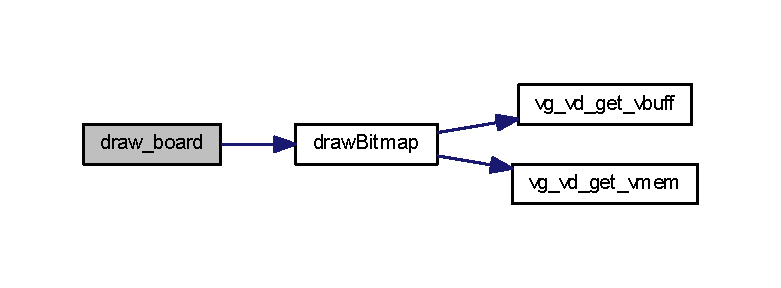
\includegraphics[width=350pt]{group___game_ga1904435b0a61ef11d90bec5376eb6398_cgraph}
\end{center}
\end{figure}
\hypertarget{group___game_ga97a9584ff1d8b78ede18e32bf5a7bd50}{}\label{group___game_ga97a9584ff1d8b78ede18e32bf5a7bd50} 
\index{Game@{Game}!init\+\_\+mouse@{init\+\_\+mouse}}
\index{init\+\_\+mouse@{init\+\_\+mouse}!Game@{Game}}
\subsubsection{\texorpdfstring{init\+\_\+mouse()}{init\_mouse()}}
{\footnotesize\ttfamily void init\+\_\+mouse (\begin{DoxyParamCaption}\item[{\hyperlink{structgame__t}{game\+\_\+t} $\ast$}]{game1 }\end{DoxyParamCaption})}



Initiates the mouse. 


\begin{DoxyParams}{Parameters}
{\em $\ast$game1} & All needed values for the game \\
\hline
\end{DoxyParams}
Here is the call graph for this function\+:
\nopagebreak
\begin{figure}[H]
\begin{center}
\leavevmode
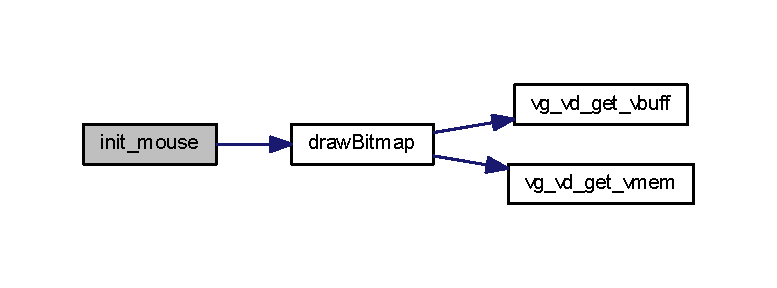
\includegraphics[width=350pt]{group___game_ga97a9584ff1d8b78ede18e32bf5a7bd50_cgraph}
\end{center}
\end{figure}
\hypertarget{group___game_ga1ebb9b5b5ce215ca81c1ca22526d935a}{}\label{group___game_ga1ebb9b5b5ce215ca81c1ca22526d935a} 
\index{Game@{Game}!init\+\_\+players@{init\+\_\+players}}
\index{init\+\_\+players@{init\+\_\+players}!Game@{Game}}
\subsubsection{\texorpdfstring{init\+\_\+players()}{init\_players()}}
{\footnotesize\ttfamily int init\+\_\+players (\begin{DoxyParamCaption}\item[{unsigned int}]{num\+\_\+players,  }\item[{\hyperlink{structgame__t}{game\+\_\+t} $\ast$}]{game1 }\end{DoxyParamCaption})}



Initiates the players. 


\begin{DoxyParams}{Parameters}
{\em num\+\_\+players} & Number of players of the game mode \\
\hline
{\em game1} & All needed values for the game \\
\hline
\end{DoxyParams}
\begin{DoxyReturn}{Returns}
Return 0 on success and 1 otherwise 
\end{DoxyReturn}


\subsection{Variable Documentation}
\hypertarget{group___game_ga2b89423d3599327880528e2d4ef4d95a}{}\label{group___game_ga2b89423d3599327880528e2d4ef4d95a} 
\index{Game@{Game}!board@{board}}
\index{board@{board}!Game@{Game}}
\subsubsection{\texorpdfstring{board}{board}}
{\footnotesize\ttfamily \hyperlink{struct_bitmap}{Bitmap}$\ast$ board}

\hypertarget{group___game_gad024627d28eb323a7677e5a265535816}{}\label{group___game_gad024627d28eb323a7677e5a265535816} 
\index{Game@{Game}!board2@{board2}}
\index{board2@{board2}!Game@{Game}}
\subsubsection{\texorpdfstring{board2}{board2}}
{\footnotesize\ttfamily \hyperlink{structboard__t}{board\+\_\+t} board2}

\hypertarget{group___game_gae6800e5869326de6be9d0be65d58b373}{}\label{group___game_gae6800e5869326de6be9d0be65d58b373} 
\index{Game@{Game}!board3@{board3}}
\index{board3@{board3}!Game@{Game}}
\subsubsection{\texorpdfstring{board3}{board3}}
{\footnotesize\ttfamily \hyperlink{structboard__t}{board\+\_\+t} board3}

\hypertarget{group___game_gadb54bfdf7a3bb4d8e2835e93b2de8a09}{}\label{group___game_gadb54bfdf7a3bb4d8e2835e93b2de8a09} 
\index{Game@{Game}!board4@{board4}}
\index{board4@{board4}!Game@{Game}}
\subsubsection{\texorpdfstring{board4}{board4}}
{\footnotesize\ttfamily \hyperlink{structboard__t}{board\+\_\+t} board4}

\hypertarget{group___game_ga39e613d7078d5537d3bbaaa3aed89f62}{}\label{group___game_ga39e613d7078d5537d3bbaaa3aed89f62} 
\index{Game@{Game}!boardp@{boardp}}
\index{boardp@{boardp}!Game@{Game}}
\subsubsection{\texorpdfstring{boardp}{boardp}}
{\footnotesize\ttfamily \hyperlink{struct_bitmap}{Bitmap} $\ast$ boardp}

\hypertarget{group___game_gab817949ca924898b4cc07f87e9936c37}{}\label{group___game_gab817949ca924898b4cc07f87e9936c37} 
\index{Game@{Game}!color1@{color1}}
\index{color1@{color1}!Game@{Game}}
\subsubsection{\texorpdfstring{color1}{color1}}
{\footnotesize\ttfamily unsigned long color1}

\hypertarget{group___game_gad66b83194e360e19ab982ad5e92c0e47}{}\label{group___game_gad66b83194e360e19ab982ad5e92c0e47} 
\index{Game@{Game}!color2@{color2}}
\index{color2@{color2}!Game@{Game}}
\subsubsection{\texorpdfstring{color2}{color2}}
{\footnotesize\ttfamily unsigned long color2}

\hypertarget{group___game_ga4a11e85efa70b04b658bbb13b38331a6}{}\label{group___game_ga4a11e85efa70b04b658bbb13b38331a6} 
\index{Game@{Game}!color3@{color3}}
\index{color3@{color3}!Game@{Game}}
\subsubsection{\texorpdfstring{color3}{color3}}
{\footnotesize\ttfamily unsigned long color3}

\hypertarget{group___game_gae4e44e3db4f37bac0f34111b5cd471d1}{}\label{group___game_gae4e44e3db4f37bac0f34111b5cd471d1} 
\index{Game@{Game}!draw@{draw}}
\index{draw@{draw}!Game@{Game}}
\subsubsection{\texorpdfstring{draw}{draw}}
{\footnotesize\ttfamily \hyperlink{struct_bitmap}{Bitmap} $\ast$ draw}

\hypertarget{group___game_gab76fa1d9cbf41273b5a8f7364a9f6f84}{}\label{group___game_gab76fa1d9cbf41273b5a8f7364a9f6f84} 
\index{Game@{Game}!gamest@{gamest}}
\index{gamest@{gamest}!Game@{Game}}
\subsubsection{\texorpdfstring{gamest}{gamest}}
{\footnotesize\ttfamily \hyperlink{group___game_ga4edce1ca040716922b6e4a79be4e414d}{game\+\_\+state\+\_\+t} gamest}

\hypertarget{group___game_ga7d15e4ad49d56102e73bfb92c6e43a22}{}\label{group___game_ga7d15e4ad49d56102e73bfb92c6e43a22} 
\index{Game@{Game}!hook\+\_\+id\+\_\+kbd@{hook\+\_\+id\+\_\+kbd}}
\index{hook\+\_\+id\+\_\+kbd@{hook\+\_\+id\+\_\+kbd}!Game@{Game}}
\subsubsection{\texorpdfstring{hook\+\_\+id\+\_\+kbd}{hook\_id\_kbd}}
{\footnotesize\ttfamily int hook\+\_\+id\+\_\+kbd}

\hypertarget{group___game_ga0b0da21bbdff62b7b28e9af7ec3d0d76}{}\label{group___game_ga0b0da21bbdff62b7b28e9af7ec3d0d76} 
\index{Game@{Game}!hook\+\_\+id\+\_\+mouse@{hook\+\_\+id\+\_\+mouse}}
\index{hook\+\_\+id\+\_\+mouse@{hook\+\_\+id\+\_\+mouse}!Game@{Game}}
\subsubsection{\texorpdfstring{hook\+\_\+id\+\_\+mouse}{hook\_id\_mouse}}
{\footnotesize\ttfamily int hook\+\_\+id\+\_\+mouse}

\hypertarget{group___game_ga7f3d11d35385878045b6b6a2ec438ba8}{}\label{group___game_ga7f3d11d35385878045b6b6a2ec438ba8} 
\index{Game@{Game}!hook\+\_\+id\+\_\+timer@{hook\+\_\+id\+\_\+timer}}
\index{hook\+\_\+id\+\_\+timer@{hook\+\_\+id\+\_\+timer}!Game@{Game}}
\subsubsection{\texorpdfstring{hook\+\_\+id\+\_\+timer}{hook\_id\_timer}}
{\footnotesize\ttfamily int hook\+\_\+id\+\_\+timer}

\hypertarget{group___game_ga492428101cf654ca73d0b290d6dc7dfc}{}\label{group___game_ga492428101cf654ca73d0b290d6dc7dfc} 
\index{Game@{Game}!irq\+\_\+set\+\_\+kbd@{irq\+\_\+set\+\_\+kbd}}
\index{irq\+\_\+set\+\_\+kbd@{irq\+\_\+set\+\_\+kbd}!Game@{Game}}
\subsubsection{\texorpdfstring{irq\+\_\+set\+\_\+kbd}{irq\_set\_kbd}}
{\footnotesize\ttfamily int irq\+\_\+set\+\_\+kbd}

\hypertarget{group___game_gafd357e4e90c5ce77865791f8e690db27}{}\label{group___game_gafd357e4e90c5ce77865791f8e690db27} 
\index{Game@{Game}!irq\+\_\+set\+\_\+mouse@{irq\+\_\+set\+\_\+mouse}}
\index{irq\+\_\+set\+\_\+mouse@{irq\+\_\+set\+\_\+mouse}!Game@{Game}}
\subsubsection{\texorpdfstring{irq\+\_\+set\+\_\+mouse}{irq\_set\_mouse}}
{\footnotesize\ttfamily int irq\+\_\+set\+\_\+mouse}

\hypertarget{group___game_gaadbf3757def1a49b68caa15ef9117b0f}{}\label{group___game_gaadbf3757def1a49b68caa15ef9117b0f} 
\index{Game@{Game}!irq\+\_\+set\+\_\+timer@{irq\+\_\+set\+\_\+timer}}
\index{irq\+\_\+set\+\_\+timer@{irq\+\_\+set\+\_\+timer}!Game@{Game}}
\subsubsection{\texorpdfstring{irq\+\_\+set\+\_\+timer}{irq\_set\_timer}}
{\footnotesize\ttfamily int irq\+\_\+set\+\_\+timer}

\hypertarget{group___game_ga74dc52caaf927df421fcbda624d6db30}{}\label{group___game_ga74dc52caaf927df421fcbda624d6db30} 
\index{Game@{Game}!left@{left}}
\index{left@{left}!Game@{Game}}
\subsubsection{\texorpdfstring{left}{left}\hspace{0.1cm}{\footnotesize\ttfamily [1/2]}}
{\footnotesize\ttfamily unsigned long left}

\hypertarget{group___game_gaecafb2f51c578021f704c30241e9032c}{}\label{group___game_gaecafb2f51c578021f704c30241e9032c} 
\index{Game@{Game}!left@{left}}
\index{left@{left}!Game@{Game}}
\subsubsection{\texorpdfstring{left}{left}\hspace{0.1cm}{\footnotesize\ttfamily [2/2]}}
{\footnotesize\ttfamily \hyperlink{group___game_gaabca14b349ba212174a00ffc1d2a2f31}{ev\+\_\+type\+\_\+t} left}

\hypertarget{group___game_ga6325f05cd0c308b41c677ec0709707a4}{}\label{group___game_ga6325f05cd0c308b41c677ec0709707a4} 
\index{Game@{Game}!lost@{lost}}
\index{lost@{lost}!Game@{Game}}
\subsubsection{\texorpdfstring{lost}{lost}\hspace{0.1cm}{\footnotesize\ttfamily [1/2]}}
{\footnotesize\ttfamily unsigned int lost}

\hypertarget{group___game_ga6325f05cd0c308b41c677ec0709707a4}{}\label{group___game_ga6325f05cd0c308b41c677ec0709707a4} 
\index{Game@{Game}!lost@{lost}}
\index{lost@{lost}!Game@{Game}}
\subsubsection{\texorpdfstring{lost}{lost}\hspace{0.1cm}{\footnotesize\ttfamily [2/2]}}
{\footnotesize\ttfamily unsigned int lost}

\hypertarget{group___game_ga4b78da9fb4428d17e14ed11877396016}{}\label{group___game_ga4b78da9fb4428d17e14ed11877396016} 
\index{Game@{Game}!menu@{menu}}
\index{menu@{menu}!Game@{Game}}
\subsubsection{\texorpdfstring{menu}{menu}}
{\footnotesize\ttfamily \hyperlink{struct_bitmap}{Bitmap} $\ast$ menu}

\hypertarget{group___game_gad10f31a0fdb4d694a65599634f4b391a}{}\label{group___game_gad10f31a0fdb4d694a65599634f4b391a} 
\index{Game@{Game}!mouse@{mouse}}
\index{mouse@{mouse}!Game@{Game}}
\subsubsection{\texorpdfstring{mouse}{mouse}}
{\footnotesize\ttfamily \hyperlink{struct_bitmap}{Bitmap} $\ast$ mouse}

\hypertarget{group___game_gab268f26e6ad9b1b9663004f9f0ea9cd4}{}\label{group___game_gab268f26e6ad9b1b9663004f9f0ea9cd4} 
\index{Game@{Game}!mouse1@{mouse1}}
\index{mouse1@{mouse1}!Game@{Game}}
\subsubsection{\texorpdfstring{mouse1}{mouse1}}
{\footnotesize\ttfamily \hyperlink{structmouse__t}{mouse\+\_\+t} mouse1}

\hypertarget{group___game_ga55cccbeadadd87a8367184083a39377a}{}\label{group___game_ga55cccbeadadd87a8367184083a39377a} 
\index{Game@{Game}!num\+\_\+players@{num\+\_\+players}}
\index{num\+\_\+players@{num\+\_\+players}!Game@{Game}}
\subsubsection{\texorpdfstring{num\+\_\+players}{num\_players}}
{\footnotesize\ttfamily unsigned int num\+\_\+players}

\hypertarget{group___game_ga948c4c379ef991ba0160f8067ee6f56b}{}\label{group___game_ga948c4c379ef991ba0160f8067ee6f56b} 
\index{Game@{Game}!paint@{paint}}
\index{paint@{paint}!Game@{Game}}
\subsubsection{\texorpdfstring{paint}{paint}}
{\footnotesize\ttfamily unsigned int paint}

\hypertarget{group___game_ga3b1e7565fd6de9b4795f4d1a2d00ec54}{}\label{group___game_ga3b1e7565fd6de9b4795f4d1a2d00ec54} 
\index{Game@{Game}!pause@{pause}}
\index{pause@{pause}!Game@{Game}}
\subsubsection{\texorpdfstring{pause}{pause}}
{\footnotesize\ttfamily \hyperlink{struct_bitmap}{Bitmap} $\ast$ pause}

\hypertarget{group___game_ga127cf5952bea43dc134fa5d96bbc0609}{}\label{group___game_ga127cf5952bea43dc134fa5d96bbc0609} 
\index{Game@{Game}!player1@{player1}}
\index{player1@{player1}!Game@{Game}}
\subsubsection{\texorpdfstring{player1}{player1}}
{\footnotesize\ttfamily \hyperlink{structplayer__t}{player\+\_\+t} player1}

\hypertarget{group___game_gaf7e237b4f038b8d3e0deea44ab5d4eff}{}\label{group___game_gaf7e237b4f038b8d3e0deea44ab5d4eff} 
\index{Game@{Game}!player2@{player2}}
\index{player2@{player2}!Game@{Game}}
\subsubsection{\texorpdfstring{player2}{player2}}
{\footnotesize\ttfamily \hyperlink{structplayer__t}{player\+\_\+t} player2}

\hypertarget{group___game_ga92766fdefc43e6eb53ca2792e05fcf51}{}\label{group___game_ga92766fdefc43e6eb53ca2792e05fcf51} 
\index{Game@{Game}!player3@{player3}}
\index{player3@{player3}!Game@{Game}}
\subsubsection{\texorpdfstring{player3}{player3}}
{\footnotesize\ttfamily \hyperlink{structplayer__t}{player\+\_\+t} player3}

\hypertarget{group___game_ga11e7b96bbf74ee5e4a0623107518f66f}{}\label{group___game_ga11e7b96bbf74ee5e4a0623107518f66f} 
\index{Game@{Game}!player4@{player4}}
\index{player4@{player4}!Game@{Game}}
\subsubsection{\texorpdfstring{player4}{player4}}
{\footnotesize\ttfamily \hyperlink{structplayer__t}{player\+\_\+t} player4}

\hypertarget{group___game_gad9567130205b4716d5412d5d936cdeb0}{}\label{group___game_gad9567130205b4716d5412d5d936cdeb0} 
\index{Game@{Game}!right@{right}}
\index{right@{right}!Game@{Game}}
\subsubsection{\texorpdfstring{right}{right}\hspace{0.1cm}{\footnotesize\ttfamily [1/2]}}
{\footnotesize\ttfamily unsigned long right}

\hypertarget{group___game_ga83501d338e4a35412684e3a442955660}{}\label{group___game_ga83501d338e4a35412684e3a442955660} 
\index{Game@{Game}!right@{right}}
\index{right@{right}!Game@{Game}}
\subsubsection{\texorpdfstring{right}{right}\hspace{0.1cm}{\footnotesize\ttfamily [2/2]}}
{\footnotesize\ttfamily \hyperlink{group___game_gaabca14b349ba212174a00ffc1d2a2f31}{ev\+\_\+type\+\_\+t} right}

\hypertarget{group___game_ga9a379079ab305d43e4c73334578f9325}{}\label{group___game_ga9a379079ab305d43e4c73334578f9325} 
\index{Game@{Game}!st@{st}}
\index{st@{st}!Game@{Game}}
\subsubsection{\texorpdfstring{st}{st}}
{\footnotesize\ttfamily \hyperlink{group___game_gaa0aafed44fec19806d8f9ad834be1248}{state\+\_\+t} st}

\hypertarget{group___game_gad50c72d4974332bda06a2cd6831b2175}{}\label{group___game_gad50c72d4974332bda06a2cd6831b2175} 
\index{Game@{Game}!start@{start}}
\index{start@{start}!Game@{Game}}
\subsubsection{\texorpdfstring{start}{start}}
{\footnotesize\ttfamily \hyperlink{struct_bitmap}{Bitmap}$\ast$ start}

\hypertarget{group___game_ga710a78637db874c6ee469e4a3f339f7f}{}\label{group___game_ga710a78637db874c6ee469e4a3f339f7f} 
\index{Game@{Game}!win@{win}}
\index{win@{win}!Game@{Game}}
\subsubsection{\texorpdfstring{win}{win}}
{\footnotesize\ttfamily \hyperlink{struct_bitmap}{Bitmap}$\ast$ win}

\hypertarget{group___game_ga676e0da0ef83bbbdf42538e54b97506b}{}\label{group___game_ga676e0da0ef83bbbdf42538e54b97506b} 
\index{Game@{Game}!x@{x}}
\index{x@{x}!Game@{Game}}
\subsubsection{\texorpdfstring{x}{x}\hspace{0.1cm}{\footnotesize\ttfamily [1/2]}}
{\footnotesize\ttfamily unsigned int x}

\hypertarget{group___game_ga676e0da0ef83bbbdf42538e54b97506b}{}\label{group___game_ga676e0da0ef83bbbdf42538e54b97506b} 
\index{Game@{Game}!x@{x}}
\index{x@{x}!Game@{Game}}
\subsubsection{\texorpdfstring{x}{x}\hspace{0.1cm}{\footnotesize\ttfamily [2/2]}}
{\footnotesize\ttfamily unsigned int x}

\hypertarget{group___game_gac30de26db5f6d1c18c63913729adca7d}{}\label{group___game_gac30de26db5f6d1c18c63913729adca7d} 
\index{Game@{Game}!y@{y}}
\index{y@{y}!Game@{Game}}
\subsubsection{\texorpdfstring{y}{y}\hspace{0.1cm}{\footnotesize\ttfamily [1/2]}}
{\footnotesize\ttfamily unsigned int y}

\hypertarget{group___game_gac30de26db5f6d1c18c63913729adca7d}{}\label{group___game_gac30de26db5f6d1c18c63913729adca7d} 
\index{Game@{Game}!y@{y}}
\index{y@{y}!Game@{Game}}
\subsubsection{\texorpdfstring{y}{y}\hspace{0.1cm}{\footnotesize\ttfamily [2/2]}}
{\footnotesize\ttfamily unsigned int y}


\hypertarget{group__vbe}{}\section{vbe}
\label{group__vbe}\index{vbe@{vbe}}
\subsection*{Data Structures}
\begin{DoxyCompactItemize}
\item 
struct \hyperlink{struct____attribute____}{\+\_\+\+\_\+attribute\+\_\+\+\_\+}
\end{DoxyCompactItemize}
\subsection*{Functions}
\begin{DoxyCompactItemize}
\item 
int \hyperlink{group__vbe_ga4ef3234e41f2050bc094a22049b69e45}{vbe\+\_\+get\+\_\+mode\+\_\+info} (unsigned short mode, vbe\+\_\+mode\+\_\+info\+\_\+t $\ast$vmi\+\_\+p)
\begin{DoxyCompactList}\small\item\em Returns information on the input V\+BE mode, including screen dimensions, color depth and V\+R\+AM physical address. \end{DoxyCompactList}\item 
int \hyperlink{group__vbe_ga04ba27e16f8dc8fb472f6f57cf66538a}{vbe\+\_\+get\+\_\+controller\+\_\+info} (Vbe\+Info\+Block $\ast$vib\+\_\+p)
\end{DoxyCompactItemize}


\subsection{Detailed Description}
Functions related to the V\+BE standard 

\subsection{Function Documentation}
\hypertarget{group__vbe_ga04ba27e16f8dc8fb472f6f57cf66538a}{}\label{group__vbe_ga04ba27e16f8dc8fb472f6f57cf66538a} 
\index{vbe@{vbe}!vbe\+\_\+get\+\_\+controller\+\_\+info@{vbe\+\_\+get\+\_\+controller\+\_\+info}}
\index{vbe\+\_\+get\+\_\+controller\+\_\+info@{vbe\+\_\+get\+\_\+controller\+\_\+info}!vbe@{vbe}}
\subsubsection{\texorpdfstring{vbe\+\_\+get\+\_\+controller\+\_\+info()}{vbe\_get\_controller\_info()}}
{\footnotesize\ttfamily int vbe\+\_\+get\+\_\+controller\+\_\+info (\begin{DoxyParamCaption}\item[{Vbe\+Info\+Block $\ast$}]{vib\+\_\+p }\end{DoxyParamCaption})}

Here is the call graph for this function\+:
\nopagebreak
\begin{figure}[H]
\begin{center}
\leavevmode
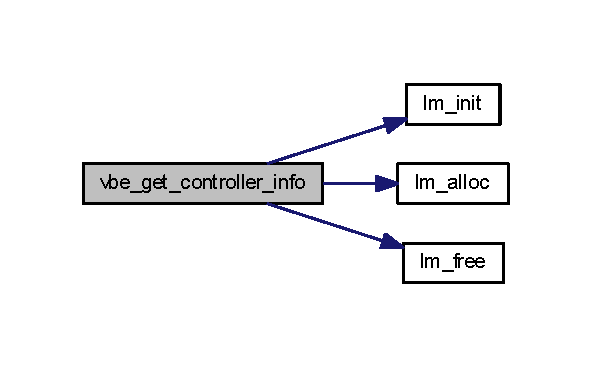
\includegraphics[width=284pt]{group__vbe_ga04ba27e16f8dc8fb472f6f57cf66538a_cgraph}
\end{center}
\end{figure}
\hypertarget{group__vbe_ga4ef3234e41f2050bc094a22049b69e45}{}\label{group__vbe_ga4ef3234e41f2050bc094a22049b69e45} 
\index{vbe@{vbe}!vbe\+\_\+get\+\_\+mode\+\_\+info@{vbe\+\_\+get\+\_\+mode\+\_\+info}}
\index{vbe\+\_\+get\+\_\+mode\+\_\+info@{vbe\+\_\+get\+\_\+mode\+\_\+info}!vbe@{vbe}}
\subsubsection{\texorpdfstring{vbe\+\_\+get\+\_\+mode\+\_\+info()}{vbe\_get\_mode\_info()}}
{\footnotesize\ttfamily int vbe\+\_\+get\+\_\+mode\+\_\+info (\begin{DoxyParamCaption}\item[{unsigned short}]{mode,  }\item[{vbe\+\_\+mode\+\_\+info\+\_\+t $\ast$}]{vmi\+\_\+p }\end{DoxyParamCaption})}



Returns information on the input V\+BE mode, including screen dimensions, color depth and V\+R\+AM physical address. 

Initializes unpacked vbe\+\_\+mode\+\_\+\+\_\+info\+\_\+t structure passed as an address with the information of the input mode, by calling V\+BE function 0x01 Return V\+BE Mode Information and unpacking the Mode\+Info\+Block struct returned by that function.


\begin{DoxyParams}{Parameters}
{\em mode} & mode whose information should be returned \\
\hline
{\em vmi\+\_\+p} & address of vbe\+\_\+mode\+\_\+info\+\_\+t structure to be initialized \\
\hline
\end{DoxyParams}
\begin{DoxyReturn}{Returns}
0 on success, non-\/zero otherwise 
\end{DoxyReturn}
Here is the call graph for this function\+:
\nopagebreak
\begin{figure}[H]
\begin{center}
\leavevmode
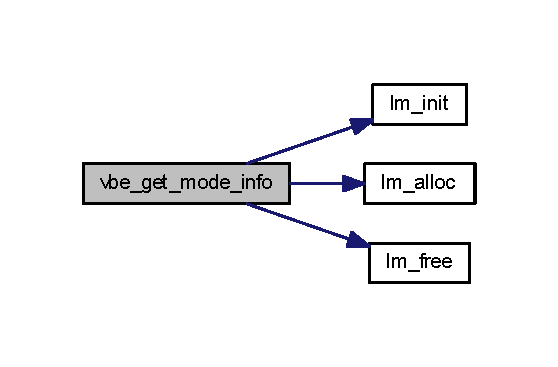
\includegraphics[width=268pt]{group__vbe_ga4ef3234e41f2050bc094a22049b69e45_cgraph}
\end{center}
\end{figure}

\hypertarget{group__video__gr}{}\section{video\+\_\+gr}
\label{group__video__gr}\index{video\+\_\+gr@{video\+\_\+gr}}
\subsection*{Functions}
\begin{DoxyCompactItemize}
\item 
void $\ast$ \hyperlink{group__video__gr_gacef21667c79365d57a084bed994c2189}{vg\+\_\+init} (unsigned short mode)
\begin{DoxyCompactList}\small\item\em Initializes the video module in graphics mode. \end{DoxyCompactList}\item 
void $\ast$ \hyperlink{group__video__gr_ga5ad1cc85a8dce3ce1a7d3e90e6ff88d3}{vg\+\_\+vd\+\_\+get\+\_\+vmem} ()
\begin{DoxyCompactList}\small\item\em Returns the Address of video\+\_\+mem. \end{DoxyCompactList}\item 
void $\ast$ \hyperlink{group__video__gr_ga3a176fda764c03218b5c20797f8b255e}{vg\+\_\+vd\+\_\+get\+\_\+vbuff} ()
\begin{DoxyCompactList}\small\item\em Returns the Address of the double buffer. \end{DoxyCompactList}\item 
void \hyperlink{group__video__gr_gab42788264b43ce014d787544fc12fdc6}{paint\+\_\+buff} ()
\begin{DoxyCompactList}\small\item\em Prints the double buffer into the video\+\_\+mem. \end{DoxyCompactList}\item 
int \hyperlink{group__video__gr_ga42f593e6656f1a978315aff02b1bcebf}{vg\+\_\+exit} (void)
\begin{DoxyCompactList}\small\item\em Returns to default Minix 3 text mode (0x03\+: 25 x 80, 16 colors) \end{DoxyCompactList}\item 
int \hyperlink{group__video__gr_gad194f7c3fabb1d2d981014ca7df5831f}{paint\+\_\+pixel} (unsigned short x, unsigned short y, unsigned long color)
\begin{DoxyCompactList}\small\item\em Paints a pixel. \end{DoxyCompactList}\item 
int \hyperlink{group__video__gr_ga3e0752b64422778fd26c0559763943b8}{paint\+\_\+pixelver} (unsigned short x, unsigned short y, unsigned long color)
\begin{DoxyCompactList}\small\item\em Paints a pixel. \end{DoxyCompactList}\item 
void \hyperlink{group__video__gr_ga4e3a822db37d5376e0c410d46bc13f95}{draw\+\_\+borders} ()
\begin{DoxyCompactList}\small\item\em Paints borders for the board. \end{DoxyCompactList}\item 
int \hyperlink{group__video__gr_gadbed0dad936e62c19d93bc8791e31527}{draw\+\_\+player} (\hyperlink{structplayer__t}{player\+\_\+t} $\ast$p, \hyperlink{group___game_gaa0aafed44fec19806d8f9ad834be1248}{state\+\_\+t} st)
\begin{DoxyCompactList}\small\item\em Draws the current position of a Player. \end{DoxyCompactList}\end{DoxyCompactItemize}


\subsection{Detailed Description}
Functions for outputing data to screen in graphics mode 

\subsection{Function Documentation}
\hypertarget{group__video__gr_ga4e3a822db37d5376e0c410d46bc13f95}{}\label{group__video__gr_ga4e3a822db37d5376e0c410d46bc13f95} 
\index{video\+\_\+gr@{video\+\_\+gr}!draw\+\_\+borders@{draw\+\_\+borders}}
\index{draw\+\_\+borders@{draw\+\_\+borders}!video\+\_\+gr@{video\+\_\+gr}}
\subsubsection{\texorpdfstring{draw\+\_\+borders()}{draw\_borders()}}
{\footnotesize\ttfamily void draw\+\_\+borders (\begin{DoxyParamCaption}{ }\end{DoxyParamCaption})}



Paints borders for the board. 

Here is the call graph for this function\+:
\nopagebreak
\begin{figure}[H]
\begin{center}
\leavevmode
\includegraphics[width=253pt]{group__video__gr_ga4e3a822db37d5376e0c410d46bc13f95_cgraph}
\end{center}
\end{figure}
\hypertarget{group__video__gr_gadbed0dad936e62c19d93bc8791e31527}{}\label{group__video__gr_gadbed0dad936e62c19d93bc8791e31527} 
\index{video\+\_\+gr@{video\+\_\+gr}!draw\+\_\+player@{draw\+\_\+player}}
\index{draw\+\_\+player@{draw\+\_\+player}!video\+\_\+gr@{video\+\_\+gr}}
\subsubsection{\texorpdfstring{draw\+\_\+player()}{draw\_player()}}
{\footnotesize\ttfamily int draw\+\_\+player (\begin{DoxyParamCaption}\item[{\hyperlink{structplayer__t}{player\+\_\+t} $\ast$}]{p,  }\item[{\hyperlink{group___game_gaa0aafed44fec19806d8f9ad834be1248}{state\+\_\+t}}]{st }\end{DoxyParamCaption})}



Draws the current position of a Player. 


\begin{DoxyParams}{Parameters}
{\em $\ast$p} & Player \\
\hline
{\em st} & State of the Player \\
\hline
\end{DoxyParams}
\begin{DoxyReturn}{Returns}
1 if the player lost and 0 if not 
\end{DoxyReturn}
Here is the call graph for this function\+:
\nopagebreak
\begin{figure}[H]
\begin{center}
\leavevmode
\includegraphics[width=259pt]{group__video__gr_gadbed0dad936e62c19d93bc8791e31527_cgraph}
\end{center}
\end{figure}
\hypertarget{group__video__gr_gab42788264b43ce014d787544fc12fdc6}{}\label{group__video__gr_gab42788264b43ce014d787544fc12fdc6} 
\index{video\+\_\+gr@{video\+\_\+gr}!paint\+\_\+buff@{paint\+\_\+buff}}
\index{paint\+\_\+buff@{paint\+\_\+buff}!video\+\_\+gr@{video\+\_\+gr}}
\subsubsection{\texorpdfstring{paint\+\_\+buff()}{paint\_buff()}}
{\footnotesize\ttfamily void paint\+\_\+buff (\begin{DoxyParamCaption}{ }\end{DoxyParamCaption})}



Prints the double buffer into the video\+\_\+mem. 

Here is the call graph for this function\+:
\nopagebreak
\begin{figure}[H]
\begin{center}
\leavevmode
\includegraphics[width=263pt]{group__video__gr_gab42788264b43ce014d787544fc12fdc6_cgraph}
\end{center}
\end{figure}
\hypertarget{group__video__gr_gad194f7c3fabb1d2d981014ca7df5831f}{}\label{group__video__gr_gad194f7c3fabb1d2d981014ca7df5831f} 
\index{video\+\_\+gr@{video\+\_\+gr}!paint\+\_\+pixel@{paint\+\_\+pixel}}
\index{paint\+\_\+pixel@{paint\+\_\+pixel}!video\+\_\+gr@{video\+\_\+gr}}
\subsubsection{\texorpdfstring{paint\+\_\+pixel()}{paint\_pixel()}}
{\footnotesize\ttfamily int paint\+\_\+pixel (\begin{DoxyParamCaption}\item[{unsigned short}]{x,  }\item[{unsigned short}]{y,  }\item[{unsigned long}]{color }\end{DoxyParamCaption})}



Paints a pixel. 


\begin{DoxyParams}{Parameters}
{\em x} & coordinate x \\
\hline
{\em y} & coordinate y \\
\hline
{\em color} & color to paint the pixel \\
\hline
\end{DoxyParams}
\begin{DoxyReturn}{Returns}
0 upon success, -\/1 if its outside of the range of video\+\_\+mem 
\end{DoxyReturn}
\hypertarget{group__video__gr_ga3e0752b64422778fd26c0559763943b8}{}\label{group__video__gr_ga3e0752b64422778fd26c0559763943b8} 
\index{video\+\_\+gr@{video\+\_\+gr}!paint\+\_\+pixelver@{paint\+\_\+pixelver}}
\index{paint\+\_\+pixelver@{paint\+\_\+pixelver}!video\+\_\+gr@{video\+\_\+gr}}
\subsubsection{\texorpdfstring{paint\+\_\+pixelver()}{paint\_pixelver()}}
{\footnotesize\ttfamily int paint\+\_\+pixelver (\begin{DoxyParamCaption}\item[{unsigned short}]{x,  }\item[{unsigned short}]{y,  }\item[{unsigned long}]{color }\end{DoxyParamCaption})}



Paints a pixel. 

Verifies before painting if its White (checking collisions)


\begin{DoxyParams}{Parameters}
{\em x} & coordinate x \\
\hline
{\em y} & coordinate y \\
\hline
{\em color} & color to paint the pixel \\
\hline
\end{DoxyParams}
\begin{DoxyReturn}{Returns}
0 upon success, -\/1 if its outside of the range of video\+\_\+mem, 1 if it was white 
\end{DoxyReturn}
\hypertarget{group__video__gr_ga42f593e6656f1a978315aff02b1bcebf}{}\label{group__video__gr_ga42f593e6656f1a978315aff02b1bcebf} 
\index{video\+\_\+gr@{video\+\_\+gr}!vg\+\_\+exit@{vg\+\_\+exit}}
\index{vg\+\_\+exit@{vg\+\_\+exit}!video\+\_\+gr@{video\+\_\+gr}}
\subsubsection{\texorpdfstring{vg\+\_\+exit()}{vg\_exit()}}
{\footnotesize\ttfamily int vg\+\_\+exit (\begin{DoxyParamCaption}\item[{void}]{ }\end{DoxyParamCaption})}



Returns to default Minix 3 text mode (0x03\+: 25 x 80, 16 colors) 

\begin{DoxyReturn}{Returns}
0 upon success, non-\/zero upon failure 
\end{DoxyReturn}
\hypertarget{group__video__gr_gacef21667c79365d57a084bed994c2189}{}\label{group__video__gr_gacef21667c79365d57a084bed994c2189} 
\index{video\+\_\+gr@{video\+\_\+gr}!vg\+\_\+init@{vg\+\_\+init}}
\index{vg\+\_\+init@{vg\+\_\+init}!video\+\_\+gr@{video\+\_\+gr}}
\subsubsection{\texorpdfstring{vg\+\_\+init()}{vg\_init()}}
{\footnotesize\ttfamily void$\ast$ vg\+\_\+init (\begin{DoxyParamCaption}\item[{unsigned short}]{mode }\end{DoxyParamCaption})}



Initializes the video module in graphics mode. 

Uses the V\+BE I\+NT 0x10 interface to set the desired graphics mode, maps V\+R\+AM to the process\textquotesingle{} address space and initializes static global variables with the resolution of the screen, and the number of colors


\begin{DoxyParams}{Parameters}
{\em mode} & 16-\/bit V\+BE mode to set \\
\hline
\end{DoxyParams}
\begin{DoxyReturn}{Returns}
Virtual address V\+R\+AM was mapped to. N\+U\+LL, upon failure. 
\end{DoxyReturn}
Here is the call graph for this function\+:
\nopagebreak
\begin{figure}[H]
\begin{center}
\leavevmode
\includegraphics[width=348pt]{group__video__gr_gacef21667c79365d57a084bed994c2189_cgraph}
\end{center}
\end{figure}
\hypertarget{group__video__gr_ga3a176fda764c03218b5c20797f8b255e}{}\label{group__video__gr_ga3a176fda764c03218b5c20797f8b255e} 
\index{video\+\_\+gr@{video\+\_\+gr}!vg\+\_\+vd\+\_\+get\+\_\+vbuff@{vg\+\_\+vd\+\_\+get\+\_\+vbuff}}
\index{vg\+\_\+vd\+\_\+get\+\_\+vbuff@{vg\+\_\+vd\+\_\+get\+\_\+vbuff}!video\+\_\+gr@{video\+\_\+gr}}
\subsubsection{\texorpdfstring{vg\+\_\+vd\+\_\+get\+\_\+vbuff()}{vg\_vd\_get\_vbuff()}}
{\footnotesize\ttfamily void$\ast$ vg\+\_\+vd\+\_\+get\+\_\+vbuff (\begin{DoxyParamCaption}{ }\end{DoxyParamCaption})}



Returns the Address of the double buffer. 

\begin{DoxyReturn}{Returns}
Returns the Address of the double buffer 
\end{DoxyReturn}
\hypertarget{group__video__gr_ga5ad1cc85a8dce3ce1a7d3e90e6ff88d3}{}\label{group__video__gr_ga5ad1cc85a8dce3ce1a7d3e90e6ff88d3} 
\index{video\+\_\+gr@{video\+\_\+gr}!vg\+\_\+vd\+\_\+get\+\_\+vmem@{vg\+\_\+vd\+\_\+get\+\_\+vmem}}
\index{vg\+\_\+vd\+\_\+get\+\_\+vmem@{vg\+\_\+vd\+\_\+get\+\_\+vmem}!video\+\_\+gr@{video\+\_\+gr}}
\subsubsection{\texorpdfstring{vg\+\_\+vd\+\_\+get\+\_\+vmem()}{vg\_vd\_get\_vmem()}}
{\footnotesize\ttfamily void$\ast$ vg\+\_\+vd\+\_\+get\+\_\+vmem (\begin{DoxyParamCaption}{ }\end{DoxyParamCaption})}



Returns the Address of video\+\_\+mem. 

\begin{DoxyReturn}{Returns}
Returns the Address of video\+\_\+mem 
\end{DoxyReturn}

\chapter{Data Structure Documentation}
\hypertarget{struct____attribute____}{}\section{\+\_\+\+\_\+attribute\+\_\+\+\_\+ Struct Reference}
\label{struct____attribute____}\index{\+\_\+\+\_\+attribute\+\_\+\+\_\+@{\+\_\+\+\_\+attribute\+\_\+\+\_\+}}


{\ttfamily \#include $<$vbe.\+h$>$}

\subsection*{Data Fields}
\begin{DoxyCompactItemize}
\item 
uint16\+\_\+t \hyperlink{struct____attribute_____ad7593abf9d201ce5e59de60baba548cd}{Mode\+Attributes}
\begin{DoxyCompactList}\small\item\em mode attributes \end{DoxyCompactList}\item 
uint8\+\_\+t \hyperlink{struct____attribute_____aaa90049ea7f03763acbbf75240f4f5d8}{Win\+A\+Attributes}
\begin{DoxyCompactList}\small\item\em window A attributes \end{DoxyCompactList}\item 
uint8\+\_\+t \hyperlink{struct____attribute_____a370ddeb84e904ef1000fe57905ebf6b8}{Win\+B\+Attributes}
\begin{DoxyCompactList}\small\item\em window B attributes \end{DoxyCompactList}\item 
uint16\+\_\+t \hyperlink{struct____attribute_____a38f205f799c6929629395f03e24de077}{Win\+Granularity}
\begin{DoxyCompactList}\small\item\em window granularity \end{DoxyCompactList}\item 
uint16\+\_\+t \hyperlink{struct____attribute_____a78985f1c5ae166cb560099273cc558b4}{Win\+Size}
\begin{DoxyCompactList}\small\item\em window size \end{DoxyCompactList}\item 
uint16\+\_\+t \hyperlink{struct____attribute_____a99b747099fd4d4271b0f0bc29f31c48f}{Win\+A\+Segment}
\begin{DoxyCompactList}\small\item\em window A start segment \end{DoxyCompactList}\item 
uint16\+\_\+t \hyperlink{struct____attribute_____a9edf422a931df7c7a1d5f82afb911566}{Win\+B\+Segment}
\begin{DoxyCompactList}\small\item\em window B start segment \end{DoxyCompactList}\item 
phys\+\_\+bytes \hyperlink{struct____attribute_____affd250a4766543099f253e27af3abc35}{Win\+Func\+Ptr}
\begin{DoxyCompactList}\small\item\em real mode/far pointer to window function \end{DoxyCompactList}\item 
uint16\+\_\+t \hyperlink{struct____attribute_____afe40654a51bf4a12a8b376ff3506688e}{Bytes\+Per\+Scan\+Line}
\begin{DoxyCompactList}\small\item\em bytes per scan line \end{DoxyCompactList}\item 
uint16\+\_\+t \hyperlink{struct____attribute_____a16f6408e5a85c7a7785a0cee64b6a219}{X\+Resolution}
\begin{DoxyCompactList}\small\item\em horizontal resolution in pixels/characters \end{DoxyCompactList}\item 
uint16\+\_\+t \hyperlink{struct____attribute_____afa8aba2156994750d500f85d0f8425cb}{Y\+Resolution}
\begin{DoxyCompactList}\small\item\em vertical resolution in pixels/characters \end{DoxyCompactList}\item 
uint8\+\_\+t \hyperlink{struct____attribute_____a047d8f41434f02589d0c9b90b17c67eb}{X\+Char\+Size}
\begin{DoxyCompactList}\small\item\em character cell width in pixels \end{DoxyCompactList}\item 
uint8\+\_\+t \hyperlink{struct____attribute_____a330f00ebd49dccd2325d43cdbd646f09}{Y\+Char\+Size}
\begin{DoxyCompactList}\small\item\em character cell height in pixels \end{DoxyCompactList}\item 
uint8\+\_\+t \hyperlink{struct____attribute_____a51268efaac55d78e17263aff9a447998}{Number\+Of\+Planes}
\begin{DoxyCompactList}\small\item\em number of memory planes \end{DoxyCompactList}\item 
uint8\+\_\+t \hyperlink{struct____attribute_____a03756ae144fce823087a2a4255bf4bb1}{Bits\+Per\+Pixel}
\begin{DoxyCompactList}\small\item\em bits per pixel \end{DoxyCompactList}\item 
uint8\+\_\+t \hyperlink{struct____attribute_____aa955c03441b6d3e55b2ba4be4dae56a2}{Number\+Of\+Banks}
\begin{DoxyCompactList}\small\item\em number of banks \end{DoxyCompactList}\item 
uint8\+\_\+t \hyperlink{struct____attribute_____ab9be703b2b515ba3428ed97af9bb084d}{Memory\+Model}
\begin{DoxyCompactList}\small\item\em memory model type \end{DoxyCompactList}\item 
uint8\+\_\+t \hyperlink{struct____attribute_____a7e31ea09e6e6755e3a504b9c76b3f545}{Bank\+Size}
\begin{DoxyCompactList}\small\item\em bank size in KB \end{DoxyCompactList}\item 
uint8\+\_\+t \hyperlink{struct____attribute_____a7033bb4cac6dc49f68ca4df855151e09}{Number\+Of\+Image\+Pages}
\begin{DoxyCompactList}\small\item\em number of images \end{DoxyCompactList}\item 
uint8\+\_\+t \hyperlink{struct____attribute_____a604037992fe7e5fd08e1bcc684a1b12d}{Reserved1}
\begin{DoxyCompactList}\small\item\em reserved for page function \end{DoxyCompactList}\item 
uint8\+\_\+t \hyperlink{struct____attribute_____a5e25f6a8eedde631fff577bcf7d4f6f4}{Red\+Mask\+Size}
\item 
uint8\+\_\+t \hyperlink{struct____attribute_____a20cb142b8c1b0a2b41244fef469a11f4}{Red\+Field\+Position}
\item 
uint8\+\_\+t \hyperlink{struct____attribute_____ac7b4df72e505b74493e7d5144cbac743}{Green\+Mask\+Size}
\item 
uint8\+\_\+t \hyperlink{struct____attribute_____a602b28f8e5da781eabfd736743a6ea09}{Green\+Field\+Position}
\item 
uint8\+\_\+t \hyperlink{struct____attribute_____a84842a6a42e881ce7be87482122bcc4e}{Blue\+Mask\+Size}
\item 
uint8\+\_\+t \hyperlink{struct____attribute_____a4d0396c07a4f07556332fec2b4a6c2bf}{Blue\+Field\+Position}
\item 
uint8\+\_\+t \hyperlink{struct____attribute_____a87d544680f1132f30b038c0ebf0b829b}{Rsvd\+Mask\+Size}
\item 
uint8\+\_\+t \hyperlink{struct____attribute_____aa357b085181776f2918a6df25c88846b}{Rsvd\+Field\+Position}
\item 
uint8\+\_\+t \hyperlink{struct____attribute_____a3bf2fd2394ec8649ec3d26104be35dd7}{Direct\+Color\+Mode\+Info}
\item 
phys\+\_\+bytes \hyperlink{struct____attribute_____a1d11f4921094db253fc2c2ee6fbb2afb}{Phys\+Base\+Ptr}
\begin{DoxyCompactList}\small\item\em physical address for flat memory frame buffer \end{DoxyCompactList}\item 
uint8\+\_\+t \hyperlink{struct____attribute_____a09b5824ec5c67bee2a4b36c0ab5181bc}{Reserved2} \mbox{[}4\mbox{]}
\begin{DoxyCompactList}\small\item\em Reserved -\/ always set to 0. \end{DoxyCompactList}\item 
uint8\+\_\+t \hyperlink{struct____attribute_____a2455a82e0d8cc0e8d76e8cf77a68bd39}{Reserved3} \mbox{[}2\mbox{]}
\begin{DoxyCompactList}\small\item\em Reserved -\/ always set to 0. \end{DoxyCompactList}\item 
uint16\+\_\+t \hyperlink{struct____attribute_____a53c5060b6ac14a7418ca8421edfb9981}{Lin\+Bytes\+Per\+Scan\+Line}
\item 
uint8\+\_\+t \hyperlink{struct____attribute_____a33ba903e149724b1bc99b3b8e43a7cbe}{Bnk\+Number\+Of\+Image\+Pages}
\item 
uint8\+\_\+t \hyperlink{struct____attribute_____a3fa2352e69836f4b69b3a344ae761ba8}{Lin\+Number\+Of\+Image\+Pages}
\item 
uint8\+\_\+t \hyperlink{struct____attribute_____a1fbcef2402fe6ce7f6c006bd50eaa6da}{Lin\+Red\+Mask\+Size}
\item 
uint8\+\_\+t \hyperlink{struct____attribute_____aff962b58f86a77f12b412d47125a4993}{Lin\+Red\+Field\+Position}
\item 
uint8\+\_\+t \hyperlink{struct____attribute_____af235e505028771ab2fb84778f4dfb476}{Lin\+Green\+Mask\+Size}
\item 
uint8\+\_\+t \hyperlink{struct____attribute_____a6683a63711dbc5dfb9a2a59c55deecd5}{Lin\+Green\+Field\+Position}
\item 
uint8\+\_\+t \hyperlink{struct____attribute_____ad8a25cec803bf91fb40a20a0aa5d5bf7}{Lin\+Blue\+Mask\+Size}
\item 
uint8\+\_\+t \hyperlink{struct____attribute_____a3f38d6becbe961786cd7ab58ec37fc07}{Lin\+Blue\+Field\+Position}
\item 
uint8\+\_\+t \hyperlink{struct____attribute_____a334886fc9a915ff91966c3aac1da586a}{Lin\+Rsvd\+Mask\+Size}
\item 
uint8\+\_\+t \hyperlink{struct____attribute_____a3df070e698b5f54814e20c8813f7bf7e}{Lin\+Rsvd\+Field\+Position}
\item 
uint32\+\_\+t \hyperlink{struct____attribute_____ab1fbd72846963ebb34a308a7edf7bbe1}{Max\+Pixel\+Clock}
\item 
uint8\+\_\+t \hyperlink{struct____attribute_____a2e13c4795a00241b919aa3aab86560ce}{Reserved4} \mbox{[}190\mbox{]}
\item 
char \hyperlink{struct____attribute_____afd3a8744ce19caa07755c2604cce884c}{Vbe\+Signature} \mbox{[}4\mbox{]}
\item 
uint16\+\_\+t \hyperlink{struct____attribute_____a7b9fef89774326b46f9481cbd9a397d3}{Vbe\+Version}
\item 
uint16\+\_\+t \hyperlink{struct____attribute_____a40bb36a43f8b3c4f8e9640007c5da428}{Oem\+String\+Ptr} \mbox{[}2\mbox{]}
\item 
uint8\+\_\+t \hyperlink{struct____attribute_____a555521aede0ff448231fc7a404862bdb}{Capabilities} \mbox{[}4\mbox{]}
\item 
uint16\+\_\+t \hyperlink{struct____attribute_____a3ae7b3b608ba57d8db68ddfa47d31d01}{Video\+Mode\+Ptr} \mbox{[}2\mbox{]}
\item 
uint16\+\_\+t \hyperlink{struct____attribute_____a3e7b41e709394a10b3667e7f27f1aa7a}{Total\+Memory}
\end{DoxyCompactItemize}


\subsection{Detailed Description}
Packed V\+BE Mode Info Block 

\subsection{Field Documentation}
\hypertarget{struct____attribute_____a7e31ea09e6e6755e3a504b9c76b3f545}{}\label{struct____attribute_____a7e31ea09e6e6755e3a504b9c76b3f545} 
\index{\+\_\+\+\_\+attribute\+\_\+\+\_\+@{\+\_\+\+\_\+attribute\+\_\+\+\_\+}!Bank\+Size@{Bank\+Size}}
\index{Bank\+Size@{Bank\+Size}!\+\_\+\+\_\+attribute\+\_\+\+\_\+@{\+\_\+\+\_\+attribute\+\_\+\+\_\+}}
\subsubsection{\texorpdfstring{Bank\+Size}{BankSize}}
{\footnotesize\ttfamily uint8\+\_\+t Bank\+Size}



bank size in KB 

\hypertarget{struct____attribute_____a03756ae144fce823087a2a4255bf4bb1}{}\label{struct____attribute_____a03756ae144fce823087a2a4255bf4bb1} 
\index{\+\_\+\+\_\+attribute\+\_\+\+\_\+@{\+\_\+\+\_\+attribute\+\_\+\+\_\+}!Bits\+Per\+Pixel@{Bits\+Per\+Pixel}}
\index{Bits\+Per\+Pixel@{Bits\+Per\+Pixel}!\+\_\+\+\_\+attribute\+\_\+\+\_\+@{\+\_\+\+\_\+attribute\+\_\+\+\_\+}}
\subsubsection{\texorpdfstring{Bits\+Per\+Pixel}{BitsPerPixel}}
{\footnotesize\ttfamily uint8\+\_\+t Bits\+Per\+Pixel}



bits per pixel 

\hypertarget{struct____attribute_____a4d0396c07a4f07556332fec2b4a6c2bf}{}\label{struct____attribute_____a4d0396c07a4f07556332fec2b4a6c2bf} 
\index{\+\_\+\+\_\+attribute\+\_\+\+\_\+@{\+\_\+\+\_\+attribute\+\_\+\+\_\+}!Blue\+Field\+Position@{Blue\+Field\+Position}}
\index{Blue\+Field\+Position@{Blue\+Field\+Position}!\+\_\+\+\_\+attribute\+\_\+\+\_\+@{\+\_\+\+\_\+attribute\+\_\+\+\_\+}}
\subsubsection{\texorpdfstring{Blue\+Field\+Position}{BlueFieldPosition}}
{\footnotesize\ttfamily uint8\+\_\+t Blue\+Field\+Position}

\hypertarget{struct____attribute_____a84842a6a42e881ce7be87482122bcc4e}{}\label{struct____attribute_____a84842a6a42e881ce7be87482122bcc4e} 
\index{\+\_\+\+\_\+attribute\+\_\+\+\_\+@{\+\_\+\+\_\+attribute\+\_\+\+\_\+}!Blue\+Mask\+Size@{Blue\+Mask\+Size}}
\index{Blue\+Mask\+Size@{Blue\+Mask\+Size}!\+\_\+\+\_\+attribute\+\_\+\+\_\+@{\+\_\+\+\_\+attribute\+\_\+\+\_\+}}
\subsubsection{\texorpdfstring{Blue\+Mask\+Size}{BlueMaskSize}}
{\footnotesize\ttfamily uint8\+\_\+t Blue\+Mask\+Size}

\hypertarget{struct____attribute_____a33ba903e149724b1bc99b3b8e43a7cbe}{}\label{struct____attribute_____a33ba903e149724b1bc99b3b8e43a7cbe} 
\index{\+\_\+\+\_\+attribute\+\_\+\+\_\+@{\+\_\+\+\_\+attribute\+\_\+\+\_\+}!Bnk\+Number\+Of\+Image\+Pages@{Bnk\+Number\+Of\+Image\+Pages}}
\index{Bnk\+Number\+Of\+Image\+Pages@{Bnk\+Number\+Of\+Image\+Pages}!\+\_\+\+\_\+attribute\+\_\+\+\_\+@{\+\_\+\+\_\+attribute\+\_\+\+\_\+}}
\subsubsection{\texorpdfstring{Bnk\+Number\+Of\+Image\+Pages}{BnkNumberOfImagePages}}
{\footnotesize\ttfamily uint8\+\_\+t Bnk\+Number\+Of\+Image\+Pages}

\hypertarget{struct____attribute_____afe40654a51bf4a12a8b376ff3506688e}{}\label{struct____attribute_____afe40654a51bf4a12a8b376ff3506688e} 
\index{\+\_\+\+\_\+attribute\+\_\+\+\_\+@{\+\_\+\+\_\+attribute\+\_\+\+\_\+}!Bytes\+Per\+Scan\+Line@{Bytes\+Per\+Scan\+Line}}
\index{Bytes\+Per\+Scan\+Line@{Bytes\+Per\+Scan\+Line}!\+\_\+\+\_\+attribute\+\_\+\+\_\+@{\+\_\+\+\_\+attribute\+\_\+\+\_\+}}
\subsubsection{\texorpdfstring{Bytes\+Per\+Scan\+Line}{BytesPerScanLine}}
{\footnotesize\ttfamily uint16\+\_\+t Bytes\+Per\+Scan\+Line}



bytes per scan line 

\hypertarget{struct____attribute_____a555521aede0ff448231fc7a404862bdb}{}\label{struct____attribute_____a555521aede0ff448231fc7a404862bdb} 
\index{\+\_\+\+\_\+attribute\+\_\+\+\_\+@{\+\_\+\+\_\+attribute\+\_\+\+\_\+}!Capabilities@{Capabilities}}
\index{Capabilities@{Capabilities}!\+\_\+\+\_\+attribute\+\_\+\+\_\+@{\+\_\+\+\_\+attribute\+\_\+\+\_\+}}
\subsubsection{\texorpdfstring{Capabilities}{Capabilities}}
{\footnotesize\ttfamily uint8\+\_\+t Capabilities\mbox{[}4\mbox{]}}

\hypertarget{struct____attribute_____a3bf2fd2394ec8649ec3d26104be35dd7}{}\label{struct____attribute_____a3bf2fd2394ec8649ec3d26104be35dd7} 
\index{\+\_\+\+\_\+attribute\+\_\+\+\_\+@{\+\_\+\+\_\+attribute\+\_\+\+\_\+}!Direct\+Color\+Mode\+Info@{Direct\+Color\+Mode\+Info}}
\index{Direct\+Color\+Mode\+Info@{Direct\+Color\+Mode\+Info}!\+\_\+\+\_\+attribute\+\_\+\+\_\+@{\+\_\+\+\_\+attribute\+\_\+\+\_\+}}
\subsubsection{\texorpdfstring{Direct\+Color\+Mode\+Info}{DirectColorModeInfo}}
{\footnotesize\ttfamily uint8\+\_\+t Direct\+Color\+Mode\+Info}

\hypertarget{struct____attribute_____a602b28f8e5da781eabfd736743a6ea09}{}\label{struct____attribute_____a602b28f8e5da781eabfd736743a6ea09} 
\index{\+\_\+\+\_\+attribute\+\_\+\+\_\+@{\+\_\+\+\_\+attribute\+\_\+\+\_\+}!Green\+Field\+Position@{Green\+Field\+Position}}
\index{Green\+Field\+Position@{Green\+Field\+Position}!\+\_\+\+\_\+attribute\+\_\+\+\_\+@{\+\_\+\+\_\+attribute\+\_\+\+\_\+}}
\subsubsection{\texorpdfstring{Green\+Field\+Position}{GreenFieldPosition}}
{\footnotesize\ttfamily uint8\+\_\+t Green\+Field\+Position}

\hypertarget{struct____attribute_____ac7b4df72e505b74493e7d5144cbac743}{}\label{struct____attribute_____ac7b4df72e505b74493e7d5144cbac743} 
\index{\+\_\+\+\_\+attribute\+\_\+\+\_\+@{\+\_\+\+\_\+attribute\+\_\+\+\_\+}!Green\+Mask\+Size@{Green\+Mask\+Size}}
\index{Green\+Mask\+Size@{Green\+Mask\+Size}!\+\_\+\+\_\+attribute\+\_\+\+\_\+@{\+\_\+\+\_\+attribute\+\_\+\+\_\+}}
\subsubsection{\texorpdfstring{Green\+Mask\+Size}{GreenMaskSize}}
{\footnotesize\ttfamily uint8\+\_\+t Green\+Mask\+Size}

\hypertarget{struct____attribute_____a3f38d6becbe961786cd7ab58ec37fc07}{}\label{struct____attribute_____a3f38d6becbe961786cd7ab58ec37fc07} 
\index{\+\_\+\+\_\+attribute\+\_\+\+\_\+@{\+\_\+\+\_\+attribute\+\_\+\+\_\+}!Lin\+Blue\+Field\+Position@{Lin\+Blue\+Field\+Position}}
\index{Lin\+Blue\+Field\+Position@{Lin\+Blue\+Field\+Position}!\+\_\+\+\_\+attribute\+\_\+\+\_\+@{\+\_\+\+\_\+attribute\+\_\+\+\_\+}}
\subsubsection{\texorpdfstring{Lin\+Blue\+Field\+Position}{LinBlueFieldPosition}}
{\footnotesize\ttfamily uint8\+\_\+t Lin\+Blue\+Field\+Position}

\hypertarget{struct____attribute_____ad8a25cec803bf91fb40a20a0aa5d5bf7}{}\label{struct____attribute_____ad8a25cec803bf91fb40a20a0aa5d5bf7} 
\index{\+\_\+\+\_\+attribute\+\_\+\+\_\+@{\+\_\+\+\_\+attribute\+\_\+\+\_\+}!Lin\+Blue\+Mask\+Size@{Lin\+Blue\+Mask\+Size}}
\index{Lin\+Blue\+Mask\+Size@{Lin\+Blue\+Mask\+Size}!\+\_\+\+\_\+attribute\+\_\+\+\_\+@{\+\_\+\+\_\+attribute\+\_\+\+\_\+}}
\subsubsection{\texorpdfstring{Lin\+Blue\+Mask\+Size}{LinBlueMaskSize}}
{\footnotesize\ttfamily uint8\+\_\+t Lin\+Blue\+Mask\+Size}

\hypertarget{struct____attribute_____a53c5060b6ac14a7418ca8421edfb9981}{}\label{struct____attribute_____a53c5060b6ac14a7418ca8421edfb9981} 
\index{\+\_\+\+\_\+attribute\+\_\+\+\_\+@{\+\_\+\+\_\+attribute\+\_\+\+\_\+}!Lin\+Bytes\+Per\+Scan\+Line@{Lin\+Bytes\+Per\+Scan\+Line}}
\index{Lin\+Bytes\+Per\+Scan\+Line@{Lin\+Bytes\+Per\+Scan\+Line}!\+\_\+\+\_\+attribute\+\_\+\+\_\+@{\+\_\+\+\_\+attribute\+\_\+\+\_\+}}
\subsubsection{\texorpdfstring{Lin\+Bytes\+Per\+Scan\+Line}{LinBytesPerScanLine}}
{\footnotesize\ttfamily uint16\+\_\+t Lin\+Bytes\+Per\+Scan\+Line}

\hypertarget{struct____attribute_____a6683a63711dbc5dfb9a2a59c55deecd5}{}\label{struct____attribute_____a6683a63711dbc5dfb9a2a59c55deecd5} 
\index{\+\_\+\+\_\+attribute\+\_\+\+\_\+@{\+\_\+\+\_\+attribute\+\_\+\+\_\+}!Lin\+Green\+Field\+Position@{Lin\+Green\+Field\+Position}}
\index{Lin\+Green\+Field\+Position@{Lin\+Green\+Field\+Position}!\+\_\+\+\_\+attribute\+\_\+\+\_\+@{\+\_\+\+\_\+attribute\+\_\+\+\_\+}}
\subsubsection{\texorpdfstring{Lin\+Green\+Field\+Position}{LinGreenFieldPosition}}
{\footnotesize\ttfamily uint8\+\_\+t Lin\+Green\+Field\+Position}

\hypertarget{struct____attribute_____af235e505028771ab2fb84778f4dfb476}{}\label{struct____attribute_____af235e505028771ab2fb84778f4dfb476} 
\index{\+\_\+\+\_\+attribute\+\_\+\+\_\+@{\+\_\+\+\_\+attribute\+\_\+\+\_\+}!Lin\+Green\+Mask\+Size@{Lin\+Green\+Mask\+Size}}
\index{Lin\+Green\+Mask\+Size@{Lin\+Green\+Mask\+Size}!\+\_\+\+\_\+attribute\+\_\+\+\_\+@{\+\_\+\+\_\+attribute\+\_\+\+\_\+}}
\subsubsection{\texorpdfstring{Lin\+Green\+Mask\+Size}{LinGreenMaskSize}}
{\footnotesize\ttfamily uint8\+\_\+t Lin\+Green\+Mask\+Size}

\hypertarget{struct____attribute_____a3fa2352e69836f4b69b3a344ae761ba8}{}\label{struct____attribute_____a3fa2352e69836f4b69b3a344ae761ba8} 
\index{\+\_\+\+\_\+attribute\+\_\+\+\_\+@{\+\_\+\+\_\+attribute\+\_\+\+\_\+}!Lin\+Number\+Of\+Image\+Pages@{Lin\+Number\+Of\+Image\+Pages}}
\index{Lin\+Number\+Of\+Image\+Pages@{Lin\+Number\+Of\+Image\+Pages}!\+\_\+\+\_\+attribute\+\_\+\+\_\+@{\+\_\+\+\_\+attribute\+\_\+\+\_\+}}
\subsubsection{\texorpdfstring{Lin\+Number\+Of\+Image\+Pages}{LinNumberOfImagePages}}
{\footnotesize\ttfamily uint8\+\_\+t Lin\+Number\+Of\+Image\+Pages}

\hypertarget{struct____attribute_____aff962b58f86a77f12b412d47125a4993}{}\label{struct____attribute_____aff962b58f86a77f12b412d47125a4993} 
\index{\+\_\+\+\_\+attribute\+\_\+\+\_\+@{\+\_\+\+\_\+attribute\+\_\+\+\_\+}!Lin\+Red\+Field\+Position@{Lin\+Red\+Field\+Position}}
\index{Lin\+Red\+Field\+Position@{Lin\+Red\+Field\+Position}!\+\_\+\+\_\+attribute\+\_\+\+\_\+@{\+\_\+\+\_\+attribute\+\_\+\+\_\+}}
\subsubsection{\texorpdfstring{Lin\+Red\+Field\+Position}{LinRedFieldPosition}}
{\footnotesize\ttfamily uint8\+\_\+t Lin\+Red\+Field\+Position}

\hypertarget{struct____attribute_____a1fbcef2402fe6ce7f6c006bd50eaa6da}{}\label{struct____attribute_____a1fbcef2402fe6ce7f6c006bd50eaa6da} 
\index{\+\_\+\+\_\+attribute\+\_\+\+\_\+@{\+\_\+\+\_\+attribute\+\_\+\+\_\+}!Lin\+Red\+Mask\+Size@{Lin\+Red\+Mask\+Size}}
\index{Lin\+Red\+Mask\+Size@{Lin\+Red\+Mask\+Size}!\+\_\+\+\_\+attribute\+\_\+\+\_\+@{\+\_\+\+\_\+attribute\+\_\+\+\_\+}}
\subsubsection{\texorpdfstring{Lin\+Red\+Mask\+Size}{LinRedMaskSize}}
{\footnotesize\ttfamily uint8\+\_\+t Lin\+Red\+Mask\+Size}

\hypertarget{struct____attribute_____a3df070e698b5f54814e20c8813f7bf7e}{}\label{struct____attribute_____a3df070e698b5f54814e20c8813f7bf7e} 
\index{\+\_\+\+\_\+attribute\+\_\+\+\_\+@{\+\_\+\+\_\+attribute\+\_\+\+\_\+}!Lin\+Rsvd\+Field\+Position@{Lin\+Rsvd\+Field\+Position}}
\index{Lin\+Rsvd\+Field\+Position@{Lin\+Rsvd\+Field\+Position}!\+\_\+\+\_\+attribute\+\_\+\+\_\+@{\+\_\+\+\_\+attribute\+\_\+\+\_\+}}
\subsubsection{\texorpdfstring{Lin\+Rsvd\+Field\+Position}{LinRsvdFieldPosition}}
{\footnotesize\ttfamily uint8\+\_\+t Lin\+Rsvd\+Field\+Position}

\hypertarget{struct____attribute_____a334886fc9a915ff91966c3aac1da586a}{}\label{struct____attribute_____a334886fc9a915ff91966c3aac1da586a} 
\index{\+\_\+\+\_\+attribute\+\_\+\+\_\+@{\+\_\+\+\_\+attribute\+\_\+\+\_\+}!Lin\+Rsvd\+Mask\+Size@{Lin\+Rsvd\+Mask\+Size}}
\index{Lin\+Rsvd\+Mask\+Size@{Lin\+Rsvd\+Mask\+Size}!\+\_\+\+\_\+attribute\+\_\+\+\_\+@{\+\_\+\+\_\+attribute\+\_\+\+\_\+}}
\subsubsection{\texorpdfstring{Lin\+Rsvd\+Mask\+Size}{LinRsvdMaskSize}}
{\footnotesize\ttfamily uint8\+\_\+t Lin\+Rsvd\+Mask\+Size}

\hypertarget{struct____attribute_____ab1fbd72846963ebb34a308a7edf7bbe1}{}\label{struct____attribute_____ab1fbd72846963ebb34a308a7edf7bbe1} 
\index{\+\_\+\+\_\+attribute\+\_\+\+\_\+@{\+\_\+\+\_\+attribute\+\_\+\+\_\+}!Max\+Pixel\+Clock@{Max\+Pixel\+Clock}}
\index{Max\+Pixel\+Clock@{Max\+Pixel\+Clock}!\+\_\+\+\_\+attribute\+\_\+\+\_\+@{\+\_\+\+\_\+attribute\+\_\+\+\_\+}}
\subsubsection{\texorpdfstring{Max\+Pixel\+Clock}{MaxPixelClock}}
{\footnotesize\ttfamily uint32\+\_\+t Max\+Pixel\+Clock}

\hypertarget{struct____attribute_____ab9be703b2b515ba3428ed97af9bb084d}{}\label{struct____attribute_____ab9be703b2b515ba3428ed97af9bb084d} 
\index{\+\_\+\+\_\+attribute\+\_\+\+\_\+@{\+\_\+\+\_\+attribute\+\_\+\+\_\+}!Memory\+Model@{Memory\+Model}}
\index{Memory\+Model@{Memory\+Model}!\+\_\+\+\_\+attribute\+\_\+\+\_\+@{\+\_\+\+\_\+attribute\+\_\+\+\_\+}}
\subsubsection{\texorpdfstring{Memory\+Model}{MemoryModel}}
{\footnotesize\ttfamily uint8\+\_\+t Memory\+Model}



memory model type 

\hypertarget{struct____attribute_____ad7593abf9d201ce5e59de60baba548cd}{}\label{struct____attribute_____ad7593abf9d201ce5e59de60baba548cd} 
\index{\+\_\+\+\_\+attribute\+\_\+\+\_\+@{\+\_\+\+\_\+attribute\+\_\+\+\_\+}!Mode\+Attributes@{Mode\+Attributes}}
\index{Mode\+Attributes@{Mode\+Attributes}!\+\_\+\+\_\+attribute\+\_\+\+\_\+@{\+\_\+\+\_\+attribute\+\_\+\+\_\+}}
\subsubsection{\texorpdfstring{Mode\+Attributes}{ModeAttributes}}
{\footnotesize\ttfamily uint16\+\_\+t Mode\+Attributes}



mode attributes 

\hypertarget{struct____attribute_____aa955c03441b6d3e55b2ba4be4dae56a2}{}\label{struct____attribute_____aa955c03441b6d3e55b2ba4be4dae56a2} 
\index{\+\_\+\+\_\+attribute\+\_\+\+\_\+@{\+\_\+\+\_\+attribute\+\_\+\+\_\+}!Number\+Of\+Banks@{Number\+Of\+Banks}}
\index{Number\+Of\+Banks@{Number\+Of\+Banks}!\+\_\+\+\_\+attribute\+\_\+\+\_\+@{\+\_\+\+\_\+attribute\+\_\+\+\_\+}}
\subsubsection{\texorpdfstring{Number\+Of\+Banks}{NumberOfBanks}}
{\footnotesize\ttfamily uint8\+\_\+t Number\+Of\+Banks}



number of banks 

\hypertarget{struct____attribute_____a7033bb4cac6dc49f68ca4df855151e09}{}\label{struct____attribute_____a7033bb4cac6dc49f68ca4df855151e09} 
\index{\+\_\+\+\_\+attribute\+\_\+\+\_\+@{\+\_\+\+\_\+attribute\+\_\+\+\_\+}!Number\+Of\+Image\+Pages@{Number\+Of\+Image\+Pages}}
\index{Number\+Of\+Image\+Pages@{Number\+Of\+Image\+Pages}!\+\_\+\+\_\+attribute\+\_\+\+\_\+@{\+\_\+\+\_\+attribute\+\_\+\+\_\+}}
\subsubsection{\texorpdfstring{Number\+Of\+Image\+Pages}{NumberOfImagePages}}
{\footnotesize\ttfamily uint8\+\_\+t Number\+Of\+Image\+Pages}



number of images 

\hypertarget{struct____attribute_____a51268efaac55d78e17263aff9a447998}{}\label{struct____attribute_____a51268efaac55d78e17263aff9a447998} 
\index{\+\_\+\+\_\+attribute\+\_\+\+\_\+@{\+\_\+\+\_\+attribute\+\_\+\+\_\+}!Number\+Of\+Planes@{Number\+Of\+Planes}}
\index{Number\+Of\+Planes@{Number\+Of\+Planes}!\+\_\+\+\_\+attribute\+\_\+\+\_\+@{\+\_\+\+\_\+attribute\+\_\+\+\_\+}}
\subsubsection{\texorpdfstring{Number\+Of\+Planes}{NumberOfPlanes}}
{\footnotesize\ttfamily uint8\+\_\+t Number\+Of\+Planes}



number of memory planes 

\hypertarget{struct____attribute_____a40bb36a43f8b3c4f8e9640007c5da428}{}\label{struct____attribute_____a40bb36a43f8b3c4f8e9640007c5da428} 
\index{\+\_\+\+\_\+attribute\+\_\+\+\_\+@{\+\_\+\+\_\+attribute\+\_\+\+\_\+}!Oem\+String\+Ptr@{Oem\+String\+Ptr}}
\index{Oem\+String\+Ptr@{Oem\+String\+Ptr}!\+\_\+\+\_\+attribute\+\_\+\+\_\+@{\+\_\+\+\_\+attribute\+\_\+\+\_\+}}
\subsubsection{\texorpdfstring{Oem\+String\+Ptr}{OemStringPtr}}
{\footnotesize\ttfamily uint16\+\_\+t Oem\+String\+Ptr\mbox{[}2\mbox{]}}

\hypertarget{struct____attribute_____a1d11f4921094db253fc2c2ee6fbb2afb}{}\label{struct____attribute_____a1d11f4921094db253fc2c2ee6fbb2afb} 
\index{\+\_\+\+\_\+attribute\+\_\+\+\_\+@{\+\_\+\+\_\+attribute\+\_\+\+\_\+}!Phys\+Base\+Ptr@{Phys\+Base\+Ptr}}
\index{Phys\+Base\+Ptr@{Phys\+Base\+Ptr}!\+\_\+\+\_\+attribute\+\_\+\+\_\+@{\+\_\+\+\_\+attribute\+\_\+\+\_\+}}
\subsubsection{\texorpdfstring{Phys\+Base\+Ptr}{PhysBasePtr}}
{\footnotesize\ttfamily phys\+\_\+bytes Phys\+Base\+Ptr}



physical address for flat memory frame buffer 

\hypertarget{struct____attribute_____a20cb142b8c1b0a2b41244fef469a11f4}{}\label{struct____attribute_____a20cb142b8c1b0a2b41244fef469a11f4} 
\index{\+\_\+\+\_\+attribute\+\_\+\+\_\+@{\+\_\+\+\_\+attribute\+\_\+\+\_\+}!Red\+Field\+Position@{Red\+Field\+Position}}
\index{Red\+Field\+Position@{Red\+Field\+Position}!\+\_\+\+\_\+attribute\+\_\+\+\_\+@{\+\_\+\+\_\+attribute\+\_\+\+\_\+}}
\subsubsection{\texorpdfstring{Red\+Field\+Position}{RedFieldPosition}}
{\footnotesize\ttfamily uint8\+\_\+t Red\+Field\+Position}

\hypertarget{struct____attribute_____a5e25f6a8eedde631fff577bcf7d4f6f4}{}\label{struct____attribute_____a5e25f6a8eedde631fff577bcf7d4f6f4} 
\index{\+\_\+\+\_\+attribute\+\_\+\+\_\+@{\+\_\+\+\_\+attribute\+\_\+\+\_\+}!Red\+Mask\+Size@{Red\+Mask\+Size}}
\index{Red\+Mask\+Size@{Red\+Mask\+Size}!\+\_\+\+\_\+attribute\+\_\+\+\_\+@{\+\_\+\+\_\+attribute\+\_\+\+\_\+}}
\subsubsection{\texorpdfstring{Red\+Mask\+Size}{RedMaskSize}}
{\footnotesize\ttfamily uint8\+\_\+t Red\+Mask\+Size}

\hypertarget{struct____attribute_____a604037992fe7e5fd08e1bcc684a1b12d}{}\label{struct____attribute_____a604037992fe7e5fd08e1bcc684a1b12d} 
\index{\+\_\+\+\_\+attribute\+\_\+\+\_\+@{\+\_\+\+\_\+attribute\+\_\+\+\_\+}!Reserved1@{Reserved1}}
\index{Reserved1@{Reserved1}!\+\_\+\+\_\+attribute\+\_\+\+\_\+@{\+\_\+\+\_\+attribute\+\_\+\+\_\+}}
\subsubsection{\texorpdfstring{Reserved1}{Reserved1}}
{\footnotesize\ttfamily uint8\+\_\+t Reserved1}



reserved for page function 

\hypertarget{struct____attribute_____a09b5824ec5c67bee2a4b36c0ab5181bc}{}\label{struct____attribute_____a09b5824ec5c67bee2a4b36c0ab5181bc} 
\index{\+\_\+\+\_\+attribute\+\_\+\+\_\+@{\+\_\+\+\_\+attribute\+\_\+\+\_\+}!Reserved2@{Reserved2}}
\index{Reserved2@{Reserved2}!\+\_\+\+\_\+attribute\+\_\+\+\_\+@{\+\_\+\+\_\+attribute\+\_\+\+\_\+}}
\subsubsection{\texorpdfstring{Reserved2}{Reserved2}}
{\footnotesize\ttfamily uint8\+\_\+t Reserved2\mbox{[}4\mbox{]}}



Reserved -\/ always set to 0. 

\hypertarget{struct____attribute_____a2455a82e0d8cc0e8d76e8cf77a68bd39}{}\label{struct____attribute_____a2455a82e0d8cc0e8d76e8cf77a68bd39} 
\index{\+\_\+\+\_\+attribute\+\_\+\+\_\+@{\+\_\+\+\_\+attribute\+\_\+\+\_\+}!Reserved3@{Reserved3}}
\index{Reserved3@{Reserved3}!\+\_\+\+\_\+attribute\+\_\+\+\_\+@{\+\_\+\+\_\+attribute\+\_\+\+\_\+}}
\subsubsection{\texorpdfstring{Reserved3}{Reserved3}}
{\footnotesize\ttfamily uint8\+\_\+t Reserved3\mbox{[}2\mbox{]}}



Reserved -\/ always set to 0. 

\hypertarget{struct____attribute_____a2e13c4795a00241b919aa3aab86560ce}{}\label{struct____attribute_____a2e13c4795a00241b919aa3aab86560ce} 
\index{\+\_\+\+\_\+attribute\+\_\+\+\_\+@{\+\_\+\+\_\+attribute\+\_\+\+\_\+}!Reserved4@{Reserved4}}
\index{Reserved4@{Reserved4}!\+\_\+\+\_\+attribute\+\_\+\+\_\+@{\+\_\+\+\_\+attribute\+\_\+\+\_\+}}
\subsubsection{\texorpdfstring{Reserved4}{Reserved4}}
{\footnotesize\ttfamily uint8\+\_\+t Reserved4\mbox{[}190\mbox{]}}

\hypertarget{struct____attribute_____aa357b085181776f2918a6df25c88846b}{}\label{struct____attribute_____aa357b085181776f2918a6df25c88846b} 
\index{\+\_\+\+\_\+attribute\+\_\+\+\_\+@{\+\_\+\+\_\+attribute\+\_\+\+\_\+}!Rsvd\+Field\+Position@{Rsvd\+Field\+Position}}
\index{Rsvd\+Field\+Position@{Rsvd\+Field\+Position}!\+\_\+\+\_\+attribute\+\_\+\+\_\+@{\+\_\+\+\_\+attribute\+\_\+\+\_\+}}
\subsubsection{\texorpdfstring{Rsvd\+Field\+Position}{RsvdFieldPosition}}
{\footnotesize\ttfamily uint8\+\_\+t Rsvd\+Field\+Position}

\hypertarget{struct____attribute_____a87d544680f1132f30b038c0ebf0b829b}{}\label{struct____attribute_____a87d544680f1132f30b038c0ebf0b829b} 
\index{\+\_\+\+\_\+attribute\+\_\+\+\_\+@{\+\_\+\+\_\+attribute\+\_\+\+\_\+}!Rsvd\+Mask\+Size@{Rsvd\+Mask\+Size}}
\index{Rsvd\+Mask\+Size@{Rsvd\+Mask\+Size}!\+\_\+\+\_\+attribute\+\_\+\+\_\+@{\+\_\+\+\_\+attribute\+\_\+\+\_\+}}
\subsubsection{\texorpdfstring{Rsvd\+Mask\+Size}{RsvdMaskSize}}
{\footnotesize\ttfamily uint8\+\_\+t Rsvd\+Mask\+Size}

\hypertarget{struct____attribute_____a3e7b41e709394a10b3667e7f27f1aa7a}{}\label{struct____attribute_____a3e7b41e709394a10b3667e7f27f1aa7a} 
\index{\+\_\+\+\_\+attribute\+\_\+\+\_\+@{\+\_\+\+\_\+attribute\+\_\+\+\_\+}!Total\+Memory@{Total\+Memory}}
\index{Total\+Memory@{Total\+Memory}!\+\_\+\+\_\+attribute\+\_\+\+\_\+@{\+\_\+\+\_\+attribute\+\_\+\+\_\+}}
\subsubsection{\texorpdfstring{Total\+Memory}{TotalMemory}}
{\footnotesize\ttfamily uint16\+\_\+t Total\+Memory}

\hypertarget{struct____attribute_____afd3a8744ce19caa07755c2604cce884c}{}\label{struct____attribute_____afd3a8744ce19caa07755c2604cce884c} 
\index{\+\_\+\+\_\+attribute\+\_\+\+\_\+@{\+\_\+\+\_\+attribute\+\_\+\+\_\+}!Vbe\+Signature@{Vbe\+Signature}}
\index{Vbe\+Signature@{Vbe\+Signature}!\+\_\+\+\_\+attribute\+\_\+\+\_\+@{\+\_\+\+\_\+attribute\+\_\+\+\_\+}}
\subsubsection{\texorpdfstring{Vbe\+Signature}{VbeSignature}}
{\footnotesize\ttfamily char Vbe\+Signature\mbox{[}4\mbox{]}}

\hypertarget{struct____attribute_____a7b9fef89774326b46f9481cbd9a397d3}{}\label{struct____attribute_____a7b9fef89774326b46f9481cbd9a397d3} 
\index{\+\_\+\+\_\+attribute\+\_\+\+\_\+@{\+\_\+\+\_\+attribute\+\_\+\+\_\+}!Vbe\+Version@{Vbe\+Version}}
\index{Vbe\+Version@{Vbe\+Version}!\+\_\+\+\_\+attribute\+\_\+\+\_\+@{\+\_\+\+\_\+attribute\+\_\+\+\_\+}}
\subsubsection{\texorpdfstring{Vbe\+Version}{VbeVersion}}
{\footnotesize\ttfamily uint16\+\_\+t Vbe\+Version}

\hypertarget{struct____attribute_____a3ae7b3b608ba57d8db68ddfa47d31d01}{}\label{struct____attribute_____a3ae7b3b608ba57d8db68ddfa47d31d01} 
\index{\+\_\+\+\_\+attribute\+\_\+\+\_\+@{\+\_\+\+\_\+attribute\+\_\+\+\_\+}!Video\+Mode\+Ptr@{Video\+Mode\+Ptr}}
\index{Video\+Mode\+Ptr@{Video\+Mode\+Ptr}!\+\_\+\+\_\+attribute\+\_\+\+\_\+@{\+\_\+\+\_\+attribute\+\_\+\+\_\+}}
\subsubsection{\texorpdfstring{Video\+Mode\+Ptr}{VideoModePtr}}
{\footnotesize\ttfamily uint16\+\_\+t Video\+Mode\+Ptr\mbox{[}2\mbox{]}}

\hypertarget{struct____attribute_____aaa90049ea7f03763acbbf75240f4f5d8}{}\label{struct____attribute_____aaa90049ea7f03763acbbf75240f4f5d8} 
\index{\+\_\+\+\_\+attribute\+\_\+\+\_\+@{\+\_\+\+\_\+attribute\+\_\+\+\_\+}!Win\+A\+Attributes@{Win\+A\+Attributes}}
\index{Win\+A\+Attributes@{Win\+A\+Attributes}!\+\_\+\+\_\+attribute\+\_\+\+\_\+@{\+\_\+\+\_\+attribute\+\_\+\+\_\+}}
\subsubsection{\texorpdfstring{Win\+A\+Attributes}{WinAAttributes}}
{\footnotesize\ttfamily uint8\+\_\+t Win\+A\+Attributes}



window A attributes 

\hypertarget{struct____attribute_____a99b747099fd4d4271b0f0bc29f31c48f}{}\label{struct____attribute_____a99b747099fd4d4271b0f0bc29f31c48f} 
\index{\+\_\+\+\_\+attribute\+\_\+\+\_\+@{\+\_\+\+\_\+attribute\+\_\+\+\_\+}!Win\+A\+Segment@{Win\+A\+Segment}}
\index{Win\+A\+Segment@{Win\+A\+Segment}!\+\_\+\+\_\+attribute\+\_\+\+\_\+@{\+\_\+\+\_\+attribute\+\_\+\+\_\+}}
\subsubsection{\texorpdfstring{Win\+A\+Segment}{WinASegment}}
{\footnotesize\ttfamily uint16\+\_\+t Win\+A\+Segment}



window A start segment 

\hypertarget{struct____attribute_____a370ddeb84e904ef1000fe57905ebf6b8}{}\label{struct____attribute_____a370ddeb84e904ef1000fe57905ebf6b8} 
\index{\+\_\+\+\_\+attribute\+\_\+\+\_\+@{\+\_\+\+\_\+attribute\+\_\+\+\_\+}!Win\+B\+Attributes@{Win\+B\+Attributes}}
\index{Win\+B\+Attributes@{Win\+B\+Attributes}!\+\_\+\+\_\+attribute\+\_\+\+\_\+@{\+\_\+\+\_\+attribute\+\_\+\+\_\+}}
\subsubsection{\texorpdfstring{Win\+B\+Attributes}{WinBAttributes}}
{\footnotesize\ttfamily uint8\+\_\+t Win\+B\+Attributes}



window B attributes 

\hypertarget{struct____attribute_____a9edf422a931df7c7a1d5f82afb911566}{}\label{struct____attribute_____a9edf422a931df7c7a1d5f82afb911566} 
\index{\+\_\+\+\_\+attribute\+\_\+\+\_\+@{\+\_\+\+\_\+attribute\+\_\+\+\_\+}!Win\+B\+Segment@{Win\+B\+Segment}}
\index{Win\+B\+Segment@{Win\+B\+Segment}!\+\_\+\+\_\+attribute\+\_\+\+\_\+@{\+\_\+\+\_\+attribute\+\_\+\+\_\+}}
\subsubsection{\texorpdfstring{Win\+B\+Segment}{WinBSegment}}
{\footnotesize\ttfamily uint16\+\_\+t Win\+B\+Segment}



window B start segment 

\hypertarget{struct____attribute_____affd250a4766543099f253e27af3abc35}{}\label{struct____attribute_____affd250a4766543099f253e27af3abc35} 
\index{\+\_\+\+\_\+attribute\+\_\+\+\_\+@{\+\_\+\+\_\+attribute\+\_\+\+\_\+}!Win\+Func\+Ptr@{Win\+Func\+Ptr}}
\index{Win\+Func\+Ptr@{Win\+Func\+Ptr}!\+\_\+\+\_\+attribute\+\_\+\+\_\+@{\+\_\+\+\_\+attribute\+\_\+\+\_\+}}
\subsubsection{\texorpdfstring{Win\+Func\+Ptr}{WinFuncPtr}}
{\footnotesize\ttfamily phys\+\_\+bytes Win\+Func\+Ptr}



real mode/far pointer to window function 

\hypertarget{struct____attribute_____a38f205f799c6929629395f03e24de077}{}\label{struct____attribute_____a38f205f799c6929629395f03e24de077} 
\index{\+\_\+\+\_\+attribute\+\_\+\+\_\+@{\+\_\+\+\_\+attribute\+\_\+\+\_\+}!Win\+Granularity@{Win\+Granularity}}
\index{Win\+Granularity@{Win\+Granularity}!\+\_\+\+\_\+attribute\+\_\+\+\_\+@{\+\_\+\+\_\+attribute\+\_\+\+\_\+}}
\subsubsection{\texorpdfstring{Win\+Granularity}{WinGranularity}}
{\footnotesize\ttfamily uint16\+\_\+t Win\+Granularity}



window granularity 

\hypertarget{struct____attribute_____a78985f1c5ae166cb560099273cc558b4}{}\label{struct____attribute_____a78985f1c5ae166cb560099273cc558b4} 
\index{\+\_\+\+\_\+attribute\+\_\+\+\_\+@{\+\_\+\+\_\+attribute\+\_\+\+\_\+}!Win\+Size@{Win\+Size}}
\index{Win\+Size@{Win\+Size}!\+\_\+\+\_\+attribute\+\_\+\+\_\+@{\+\_\+\+\_\+attribute\+\_\+\+\_\+}}
\subsubsection{\texorpdfstring{Win\+Size}{WinSize}}
{\footnotesize\ttfamily uint16\+\_\+t Win\+Size}



window size 

\hypertarget{struct____attribute_____a047d8f41434f02589d0c9b90b17c67eb}{}\label{struct____attribute_____a047d8f41434f02589d0c9b90b17c67eb} 
\index{\+\_\+\+\_\+attribute\+\_\+\+\_\+@{\+\_\+\+\_\+attribute\+\_\+\+\_\+}!X\+Char\+Size@{X\+Char\+Size}}
\index{X\+Char\+Size@{X\+Char\+Size}!\+\_\+\+\_\+attribute\+\_\+\+\_\+@{\+\_\+\+\_\+attribute\+\_\+\+\_\+}}
\subsubsection{\texorpdfstring{X\+Char\+Size}{XCharSize}}
{\footnotesize\ttfamily uint8\+\_\+t X\+Char\+Size}



character cell width in pixels 

\hypertarget{struct____attribute_____a16f6408e5a85c7a7785a0cee64b6a219}{}\label{struct____attribute_____a16f6408e5a85c7a7785a0cee64b6a219} 
\index{\+\_\+\+\_\+attribute\+\_\+\+\_\+@{\+\_\+\+\_\+attribute\+\_\+\+\_\+}!X\+Resolution@{X\+Resolution}}
\index{X\+Resolution@{X\+Resolution}!\+\_\+\+\_\+attribute\+\_\+\+\_\+@{\+\_\+\+\_\+attribute\+\_\+\+\_\+}}
\subsubsection{\texorpdfstring{X\+Resolution}{XResolution}}
{\footnotesize\ttfamily uint16\+\_\+t X\+Resolution}



horizontal resolution in pixels/characters 

\hypertarget{struct____attribute_____a330f00ebd49dccd2325d43cdbd646f09}{}\label{struct____attribute_____a330f00ebd49dccd2325d43cdbd646f09} 
\index{\+\_\+\+\_\+attribute\+\_\+\+\_\+@{\+\_\+\+\_\+attribute\+\_\+\+\_\+}!Y\+Char\+Size@{Y\+Char\+Size}}
\index{Y\+Char\+Size@{Y\+Char\+Size}!\+\_\+\+\_\+attribute\+\_\+\+\_\+@{\+\_\+\+\_\+attribute\+\_\+\+\_\+}}
\subsubsection{\texorpdfstring{Y\+Char\+Size}{YCharSize}}
{\footnotesize\ttfamily uint8\+\_\+t Y\+Char\+Size}



character cell height in pixels 

\hypertarget{struct____attribute_____afa8aba2156994750d500f85d0f8425cb}{}\label{struct____attribute_____afa8aba2156994750d500f85d0f8425cb} 
\index{\+\_\+\+\_\+attribute\+\_\+\+\_\+@{\+\_\+\+\_\+attribute\+\_\+\+\_\+}!Y\+Resolution@{Y\+Resolution}}
\index{Y\+Resolution@{Y\+Resolution}!\+\_\+\+\_\+attribute\+\_\+\+\_\+@{\+\_\+\+\_\+attribute\+\_\+\+\_\+}}
\subsubsection{\texorpdfstring{Y\+Resolution}{YResolution}}
{\footnotesize\ttfamily uint16\+\_\+t Y\+Resolution}



vertical resolution in pixels/characters 



The documentation for this struct was generated from the following file\+:\begin{DoxyCompactItemize}
\item 
C\+:/\+Users/jnuno/\+Desktop/src/\hyperlink{vbe_8h}{vbe.\+h}\end{DoxyCompactItemize}

\hypertarget{struct_bitmap}{}\section{Bitmap Struct Reference}
\label{struct_bitmap}\index{Bitmap@{Bitmap}}


Represents a \hyperlink{struct_bitmap}{Bitmap}.  




{\ttfamily \#include $<$read\+\_\+bitmap.\+h$>$}



Collaboration diagram for Bitmap\+:
\nopagebreak
\begin{figure}[H]
\begin{center}
\leavevmode
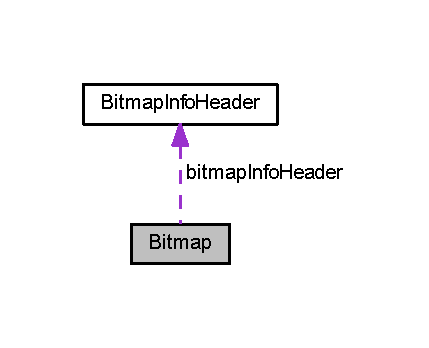
\includegraphics[width=206pt]{struct_bitmap__coll__graph}
\end{center}
\end{figure}
\subsection*{Data Fields}
\begin{DoxyCompactItemize}
\item 
\hyperlink{struct_bitmap_info_header}{Bitmap\+Info\+Header} \hyperlink{struct_bitmap_a7157ca7f3ce4be47481c472fafd89313}{bitmap\+Info\+Header}
\item 
unsigned char $\ast$ \hyperlink{struct_bitmap_a586c4bcc42cf22a033e8f60f24f627f0}{bitmap\+Data}
\end{DoxyCompactItemize}


\subsection{Detailed Description}
Represents a \hyperlink{struct_bitmap}{Bitmap}. 

\subsection{Field Documentation}
\hypertarget{struct_bitmap_a586c4bcc42cf22a033e8f60f24f627f0}{}\label{struct_bitmap_a586c4bcc42cf22a033e8f60f24f627f0} 
\index{Bitmap@{Bitmap}!bitmap\+Data@{bitmap\+Data}}
\index{bitmap\+Data@{bitmap\+Data}!Bitmap@{Bitmap}}
\subsubsection{\texorpdfstring{bitmap\+Data}{bitmapData}}
{\footnotesize\ttfamily unsigned char$\ast$ bitmap\+Data}

\hypertarget{struct_bitmap_a7157ca7f3ce4be47481c472fafd89313}{}\label{struct_bitmap_a7157ca7f3ce4be47481c472fafd89313} 
\index{Bitmap@{Bitmap}!bitmap\+Info\+Header@{bitmap\+Info\+Header}}
\index{bitmap\+Info\+Header@{bitmap\+Info\+Header}!Bitmap@{Bitmap}}
\subsubsection{\texorpdfstring{bitmap\+Info\+Header}{bitmapInfoHeader}}
{\footnotesize\ttfamily \hyperlink{struct_bitmap_info_header}{Bitmap\+Info\+Header} bitmap\+Info\+Header}



The documentation for this struct was generated from the following file\+:\begin{DoxyCompactItemize}
\item 
C\+:/\+Users/jnuno/\+Desktop/src/\hyperlink{read__bitmap_8h}{read\+\_\+bitmap.\+h}\end{DoxyCompactItemize}

\hypertarget{struct_bitmap_file_header}{}\section{Bitmap\+File\+Header Struct Reference}
\label{struct_bitmap_file_header}\index{Bitmap\+File\+Header@{Bitmap\+File\+Header}}


{\ttfamily \#include $<$read\+\_\+bitmap.\+h$>$}

\subsection*{Data Fields}
\begin{DoxyCompactItemize}
\item 
unsigned short \hyperlink{struct_bitmap_file_header_aa929142c5ddf34cf0915c97a617a1a63}{type}
\item 
unsigned int \hyperlink{struct_bitmap_file_header_aac913b3a1f6ef005d66bf7a84428773e}{size}
\item 
unsigned int \hyperlink{struct_bitmap_file_header_a05d5cbcb44f437341bd9fa37d589aced}{reserved}
\item 
unsigned int \hyperlink{struct_bitmap_file_header_a29b5297d3393519050e3126c4cb07c1c}{offset}
\end{DoxyCompactItemize}


\subsection{Field Documentation}
\hypertarget{struct_bitmap_file_header_a29b5297d3393519050e3126c4cb07c1c}{}\label{struct_bitmap_file_header_a29b5297d3393519050e3126c4cb07c1c} 
\index{Bitmap\+File\+Header@{Bitmap\+File\+Header}!offset@{offset}}
\index{offset@{offset}!Bitmap\+File\+Header@{Bitmap\+File\+Header}}
\subsubsection{\texorpdfstring{offset}{offset}}
{\footnotesize\ttfamily unsigned int offset}

\hypertarget{struct_bitmap_file_header_a05d5cbcb44f437341bd9fa37d589aced}{}\label{struct_bitmap_file_header_a05d5cbcb44f437341bd9fa37d589aced} 
\index{Bitmap\+File\+Header@{Bitmap\+File\+Header}!reserved@{reserved}}
\index{reserved@{reserved}!Bitmap\+File\+Header@{Bitmap\+File\+Header}}
\subsubsection{\texorpdfstring{reserved}{reserved}}
{\footnotesize\ttfamily unsigned int reserved}

\hypertarget{struct_bitmap_file_header_aac913b3a1f6ef005d66bf7a84428773e}{}\label{struct_bitmap_file_header_aac913b3a1f6ef005d66bf7a84428773e} 
\index{Bitmap\+File\+Header@{Bitmap\+File\+Header}!size@{size}}
\index{size@{size}!Bitmap\+File\+Header@{Bitmap\+File\+Header}}
\subsubsection{\texorpdfstring{size}{size}}
{\footnotesize\ttfamily unsigned int size}

\hypertarget{struct_bitmap_file_header_aa929142c5ddf34cf0915c97a617a1a63}{}\label{struct_bitmap_file_header_aa929142c5ddf34cf0915c97a617a1a63} 
\index{Bitmap\+File\+Header@{Bitmap\+File\+Header}!type@{type}}
\index{type@{type}!Bitmap\+File\+Header@{Bitmap\+File\+Header}}
\subsubsection{\texorpdfstring{type}{type}}
{\footnotesize\ttfamily unsigned short type}



The documentation for this struct was generated from the following file\+:\begin{DoxyCompactItemize}
\item 
C\+:/\+Users/jnuno/\+Desktop/src/\hyperlink{read__bitmap_8h}{read\+\_\+bitmap.\+h}\end{DoxyCompactItemize}

\hypertarget{struct_bitmap_info_header}{}\section{Bitmap\+Info\+Header Struct Reference}
\label{struct_bitmap_info_header}\index{Bitmap\+Info\+Header@{Bitmap\+Info\+Header}}


{\ttfamily \#include $<$read\+\_\+bitmap.\+h$>$}

\subsection*{Data Fields}
\begin{DoxyCompactItemize}
\item 
unsigned int \hyperlink{struct_bitmap_info_header_aac913b3a1f6ef005d66bf7a84428773e}{size}
\item 
int \hyperlink{struct_bitmap_info_header_a2474a5474cbff19523a51eb1de01cda4}{width}
\item 
int \hyperlink{struct_bitmap_info_header_ad12fc34ce789bce6c8a05d8a17138534}{height}
\item 
unsigned short \hyperlink{struct_bitmap_info_header_a8c89d091e05544a82dc2398eed99634f}{planes}
\item 
unsigned short \hyperlink{struct_bitmap_info_header_a47d1d4d776f8fd3bb0f7dbc3c5aeb534}{bits}
\item 
unsigned int \hyperlink{struct_bitmap_info_header_ad180079f62b44e49ec672c9ef6e078b3}{compression}
\item 
unsigned int \hyperlink{struct_bitmap_info_header_adcd57a0168319e747bc8099218d3822c}{image\+Size}
\item 
int \hyperlink{struct_bitmap_info_header_ac6eaeb4c0876cf6cd899f41fe3c25ff5}{x\+Resolution}
\item 
int \hyperlink{struct_bitmap_info_header_aa2f350dd0bda750656d5db5f5e37b2b3}{y\+Resolution}
\item 
unsigned int \hyperlink{struct_bitmap_info_header_aed4506bad904845183194f199f1bdb98}{n\+Colors}
\item 
unsigned int \hyperlink{struct_bitmap_info_header_a8f7abfbc446b12f385d2b42c3b4fd9b0}{important\+Colors}
\end{DoxyCompactItemize}


\subsection{Field Documentation}
\hypertarget{struct_bitmap_info_header_a47d1d4d776f8fd3bb0f7dbc3c5aeb534}{}\label{struct_bitmap_info_header_a47d1d4d776f8fd3bb0f7dbc3c5aeb534} 
\index{Bitmap\+Info\+Header@{Bitmap\+Info\+Header}!bits@{bits}}
\index{bits@{bits}!Bitmap\+Info\+Header@{Bitmap\+Info\+Header}}
\subsubsection{\texorpdfstring{bits}{bits}}
{\footnotesize\ttfamily unsigned short bits}

\hypertarget{struct_bitmap_info_header_ad180079f62b44e49ec672c9ef6e078b3}{}\label{struct_bitmap_info_header_ad180079f62b44e49ec672c9ef6e078b3} 
\index{Bitmap\+Info\+Header@{Bitmap\+Info\+Header}!compression@{compression}}
\index{compression@{compression}!Bitmap\+Info\+Header@{Bitmap\+Info\+Header}}
\subsubsection{\texorpdfstring{compression}{compression}}
{\footnotesize\ttfamily unsigned int compression}

\hypertarget{struct_bitmap_info_header_ad12fc34ce789bce6c8a05d8a17138534}{}\label{struct_bitmap_info_header_ad12fc34ce789bce6c8a05d8a17138534} 
\index{Bitmap\+Info\+Header@{Bitmap\+Info\+Header}!height@{height}}
\index{height@{height}!Bitmap\+Info\+Header@{Bitmap\+Info\+Header}}
\subsubsection{\texorpdfstring{height}{height}}
{\footnotesize\ttfamily int height}

\hypertarget{struct_bitmap_info_header_adcd57a0168319e747bc8099218d3822c}{}\label{struct_bitmap_info_header_adcd57a0168319e747bc8099218d3822c} 
\index{Bitmap\+Info\+Header@{Bitmap\+Info\+Header}!image\+Size@{image\+Size}}
\index{image\+Size@{image\+Size}!Bitmap\+Info\+Header@{Bitmap\+Info\+Header}}
\subsubsection{\texorpdfstring{image\+Size}{imageSize}}
{\footnotesize\ttfamily unsigned int image\+Size}

\hypertarget{struct_bitmap_info_header_a8f7abfbc446b12f385d2b42c3b4fd9b0}{}\label{struct_bitmap_info_header_a8f7abfbc446b12f385d2b42c3b4fd9b0} 
\index{Bitmap\+Info\+Header@{Bitmap\+Info\+Header}!important\+Colors@{important\+Colors}}
\index{important\+Colors@{important\+Colors}!Bitmap\+Info\+Header@{Bitmap\+Info\+Header}}
\subsubsection{\texorpdfstring{important\+Colors}{importantColors}}
{\footnotesize\ttfamily unsigned int important\+Colors}

\hypertarget{struct_bitmap_info_header_aed4506bad904845183194f199f1bdb98}{}\label{struct_bitmap_info_header_aed4506bad904845183194f199f1bdb98} 
\index{Bitmap\+Info\+Header@{Bitmap\+Info\+Header}!n\+Colors@{n\+Colors}}
\index{n\+Colors@{n\+Colors}!Bitmap\+Info\+Header@{Bitmap\+Info\+Header}}
\subsubsection{\texorpdfstring{n\+Colors}{nColors}}
{\footnotesize\ttfamily unsigned int n\+Colors}

\hypertarget{struct_bitmap_info_header_a8c89d091e05544a82dc2398eed99634f}{}\label{struct_bitmap_info_header_a8c89d091e05544a82dc2398eed99634f} 
\index{Bitmap\+Info\+Header@{Bitmap\+Info\+Header}!planes@{planes}}
\index{planes@{planes}!Bitmap\+Info\+Header@{Bitmap\+Info\+Header}}
\subsubsection{\texorpdfstring{planes}{planes}}
{\footnotesize\ttfamily unsigned short planes}

\hypertarget{struct_bitmap_info_header_aac913b3a1f6ef005d66bf7a84428773e}{}\label{struct_bitmap_info_header_aac913b3a1f6ef005d66bf7a84428773e} 
\index{Bitmap\+Info\+Header@{Bitmap\+Info\+Header}!size@{size}}
\index{size@{size}!Bitmap\+Info\+Header@{Bitmap\+Info\+Header}}
\subsubsection{\texorpdfstring{size}{size}}
{\footnotesize\ttfamily unsigned int size}

\hypertarget{struct_bitmap_info_header_a2474a5474cbff19523a51eb1de01cda4}{}\label{struct_bitmap_info_header_a2474a5474cbff19523a51eb1de01cda4} 
\index{Bitmap\+Info\+Header@{Bitmap\+Info\+Header}!width@{width}}
\index{width@{width}!Bitmap\+Info\+Header@{Bitmap\+Info\+Header}}
\subsubsection{\texorpdfstring{width}{width}}
{\footnotesize\ttfamily int width}

\hypertarget{struct_bitmap_info_header_ac6eaeb4c0876cf6cd899f41fe3c25ff5}{}\label{struct_bitmap_info_header_ac6eaeb4c0876cf6cd899f41fe3c25ff5} 
\index{Bitmap\+Info\+Header@{Bitmap\+Info\+Header}!x\+Resolution@{x\+Resolution}}
\index{x\+Resolution@{x\+Resolution}!Bitmap\+Info\+Header@{Bitmap\+Info\+Header}}
\subsubsection{\texorpdfstring{x\+Resolution}{xResolution}}
{\footnotesize\ttfamily int x\+Resolution}

\hypertarget{struct_bitmap_info_header_aa2f350dd0bda750656d5db5f5e37b2b3}{}\label{struct_bitmap_info_header_aa2f350dd0bda750656d5db5f5e37b2b3} 
\index{Bitmap\+Info\+Header@{Bitmap\+Info\+Header}!y\+Resolution@{y\+Resolution}}
\index{y\+Resolution@{y\+Resolution}!Bitmap\+Info\+Header@{Bitmap\+Info\+Header}}
\subsubsection{\texorpdfstring{y\+Resolution}{yResolution}}
{\footnotesize\ttfamily int y\+Resolution}



The documentation for this struct was generated from the following file\+:\begin{DoxyCompactItemize}
\item 
C\+:/\+Users/jnuno/\+Desktop/src/\hyperlink{read__bitmap_8h}{read\+\_\+bitmap.\+h}\end{DoxyCompactItemize}

\hypertarget{structboard__t}{}\section{board\+\_\+t Struct Reference}
\label{structboard__t}\index{board\+\_\+t@{board\+\_\+t}}


{\ttfamily \#include $<$tools.\+h$>$}



Collaboration diagram for board\+\_\+t\+:
\nopagebreak
\begin{figure}[H]
\begin{center}
\leavevmode
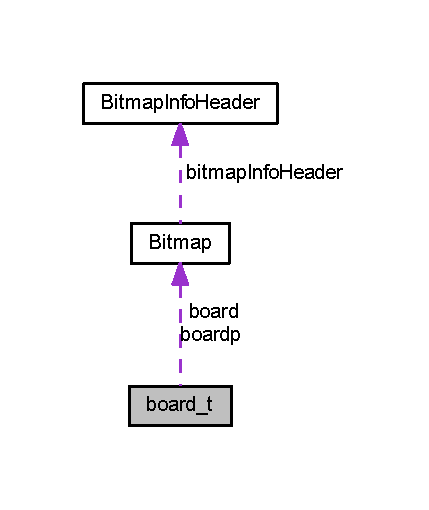
\includegraphics[width=206pt]{structboard__t__coll__graph}
\end{center}
\end{figure}
\subsection*{Data Fields}
\begin{DoxyCompactItemize}
\item 
\hyperlink{struct_bitmap}{Bitmap} $\ast$ \hyperlink{group___game_ga2b89423d3599327880528e2d4ef4d95a}{board}
\item 
\hyperlink{struct_bitmap}{Bitmap} $\ast$ \hyperlink{group___game_ga39e613d7078d5537d3bbaaa3aed89f62}{boardp}
\end{DoxyCompactItemize}


The documentation for this struct was generated from the following file\+:\begin{DoxyCompactItemize}
\item 
C\+:/\+Users/jnuno/\+Desktop/src/\hyperlink{tools_8h}{tools.\+h}\end{DoxyCompactItemize}

\hypertarget{structgame__t}{}\section{game\+\_\+t Struct Reference}
\label{structgame__t}\index{game\+\_\+t@{game\+\_\+t}}


{\ttfamily \#include $<$tools.\+h$>$}



Collaboration diagram for game\+\_\+t\+:
\nopagebreak
\begin{figure}[H]
\begin{center}
\leavevmode
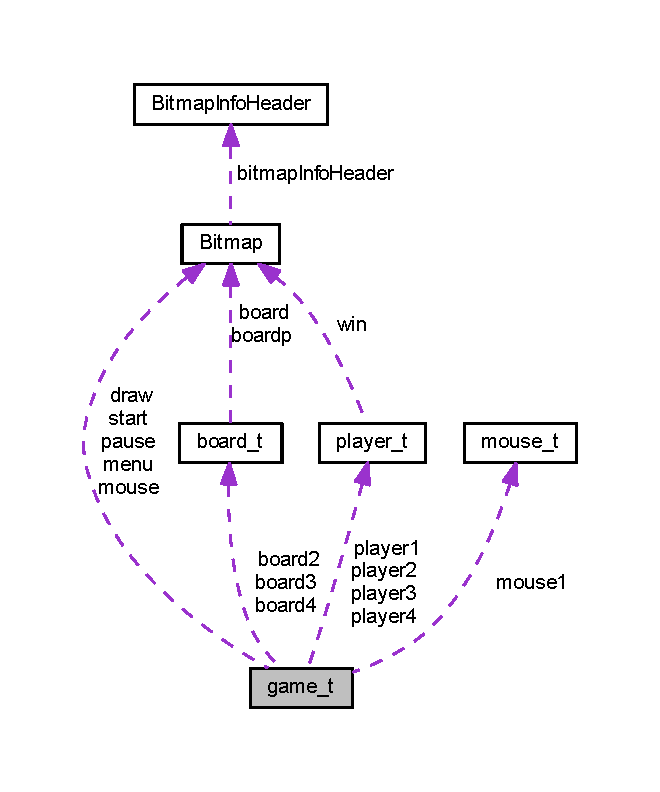
\includegraphics[width=317pt]{structgame__t__coll__graph}
\end{center}
\end{figure}
\subsection*{Data Fields}
\begin{DoxyCompactItemize}
\item 
\hyperlink{group___game_ga4edce1ca040716922b6e4a79be4e414d}{game\+\_\+state\+\_\+t} \hyperlink{group___game_gab76fa1d9cbf41273b5a8f7364a9f6f84}{gamest}
\item 
\hyperlink{structplayer__t}{player\+\_\+t} \hyperlink{group___game_ga127cf5952bea43dc134fa5d96bbc0609}{player1}
\item 
\hyperlink{structplayer__t}{player\+\_\+t} \hyperlink{group___game_gaf7e237b4f038b8d3e0deea44ab5d4eff}{player2}
\item 
\hyperlink{structplayer__t}{player\+\_\+t} \hyperlink{group___game_ga92766fdefc43e6eb53ca2792e05fcf51}{player3}
\item 
\hyperlink{structplayer__t}{player\+\_\+t} \hyperlink{group___game_ga11e7b96bbf74ee5e4a0623107518f66f}{player4}
\item 
\hyperlink{structmouse__t}{mouse\+\_\+t} \hyperlink{group___game_gab268f26e6ad9b1b9663004f9f0ea9cd4}{mouse1}
\item 
unsigned int \hyperlink{group___game_ga55cccbeadadd87a8367184083a39377a}{num\+\_\+players}
\item 
unsigned int \hyperlink{group___game_ga6325f05cd0c308b41c677ec0709707a4}{lost}
\item 
int \hyperlink{group___game_ga7f3d11d35385878045b6b6a2ec438ba8}{hook\+\_\+id\+\_\+timer}
\item 
int \hyperlink{group___game_gaadbf3757def1a49b68caa15ef9117b0f}{irq\+\_\+set\+\_\+timer}
\item 
int \hyperlink{group___game_ga7d15e4ad49d56102e73bfb92c6e43a22}{hook\+\_\+id\+\_\+kbd}
\item 
int \hyperlink{group___game_ga492428101cf654ca73d0b290d6dc7dfc}{irq\+\_\+set\+\_\+kbd}
\item 
int \hyperlink{group___game_ga0b0da21bbdff62b7b28e9af7ec3d0d76}{hook\+\_\+id\+\_\+mouse}
\item 
int \hyperlink{group___game_gafd357e4e90c5ce77865791f8e690db27}{irq\+\_\+set\+\_\+mouse}
\item 
\hyperlink{structboard__t}{board\+\_\+t} \hyperlink{group___game_gad024627d28eb323a7677e5a265535816}{board2}
\item 
\hyperlink{structboard__t}{board\+\_\+t} \hyperlink{group___game_gae6800e5869326de6be9d0be65d58b373}{board3}
\item 
\hyperlink{structboard__t}{board\+\_\+t} \hyperlink{group___game_gadb54bfdf7a3bb4d8e2835e93b2de8a09}{board4}
\item 
\hyperlink{struct_bitmap}{Bitmap} $\ast$ \hyperlink{group___game_gad50c72d4974332bda06a2cd6831b2175}{start}
\item 
\hyperlink{struct_bitmap}{Bitmap} $\ast$ \hyperlink{group___game_gad10f31a0fdb4d694a65599634f4b391a}{mouse}
\item 
\hyperlink{struct_bitmap}{Bitmap} $\ast$ \hyperlink{group___game_ga4b78da9fb4428d17e14ed11877396016}{menu}
\item 
\hyperlink{struct_bitmap}{Bitmap} $\ast$ \hyperlink{group___game_ga3b1e7565fd6de9b4795f4d1a2d00ec54}{pause}
\item 
\hyperlink{struct_bitmap}{Bitmap} $\ast$ \hyperlink{group___game_gae4e44e3db4f37bac0f34111b5cd471d1}{draw}
\end{DoxyCompactItemize}


The documentation for this struct was generated from the following file\+:\begin{DoxyCompactItemize}
\item 
C\+:/\+Users/jnuno/\+Desktop/src/\hyperlink{tools_8h}{tools.\+h}\end{DoxyCompactItemize}

\hypertarget{structmmap__t}{}\section{mmap\+\_\+t Struct Reference}
\label{structmmap__t}\index{mmap\+\_\+t@{mmap\+\_\+t}}


{\ttfamily \#include $<$lmlib.\+h$>$}

\subsection*{Data Fields}
\begin{DoxyCompactItemize}
\item 
phys\+\_\+bytes \hyperlink{group__lmlib_gab7a85fe0db943529016cf606e3a7167f}{phys}
\begin{DoxyCompactList}\small\item\em physical address \end{DoxyCompactList}\item 
void $\ast$ \hyperlink{group__lmlib_ga6a0ea2231d30f2b025e0c4b9f12dd6db}{virtual}
\begin{DoxyCompactList}\small\item\em virtual address \end{DoxyCompactList}\item 
unsigned long \hyperlink{group__lmlib_ga1e1268d164c38e4f8a4f4eb9058b0601}{size}
\begin{DoxyCompactList}\small\item\em size of memory region \end{DoxyCompactList}\end{DoxyCompactItemize}


\subsection{Detailed Description}
Struct that keeps info regarding the mapping of physical memory to virtual memory 

The documentation for this struct was generated from the following file\+:\begin{DoxyCompactItemize}
\item 
C\+:/\+Users/jnuno/\+Desktop/src/\hyperlink{lmlib_8h}{lmlib.\+h}\end{DoxyCompactItemize}

\hypertarget{structmouse__t}{}\section{mouse\+\_\+t Struct Reference}
\label{structmouse__t}\index{mouse\+\_\+t@{mouse\+\_\+t}}


{\ttfamily \#include $<$tools.\+h$>$}

\subsection*{Data Fields}
\begin{DoxyCompactItemize}
\item 
unsigned int \hyperlink{group___game_ga676e0da0ef83bbbdf42538e54b97506b}{x}
\item 
unsigned int \hyperlink{group___game_gac30de26db5f6d1c18c63913729adca7d}{y}
\item 
unsigned int \hyperlink{group___game_ga948c4c379ef991ba0160f8067ee6f56b}{paint}
\item 
\hyperlink{group___game_gaabca14b349ba212174a00ffc1d2a2f31}{ev\+\_\+type\+\_\+t} \hyperlink{group___game_gaecafb2f51c578021f704c30241e9032c}{left}
\item 
\hyperlink{group___game_gaabca14b349ba212174a00ffc1d2a2f31}{ev\+\_\+type\+\_\+t} \hyperlink{group___game_ga83501d338e4a35412684e3a442955660}{right}
\end{DoxyCompactItemize}


The documentation for this struct was generated from the following file\+:\begin{DoxyCompactItemize}
\item 
C\+:/\+Users/jnuno/\+Desktop/src/\hyperlink{tools_8h}{tools.\+h}\end{DoxyCompactItemize}

\hypertarget{structplayer__t}{}\section{player\+\_\+t Struct Reference}
\label{structplayer__t}\index{player\+\_\+t@{player\+\_\+t}}


{\ttfamily \#include $<$tools.\+h$>$}



Collaboration diagram for player\+\_\+t\+:
\nopagebreak
\begin{figure}[H]
\begin{center}
\leavevmode
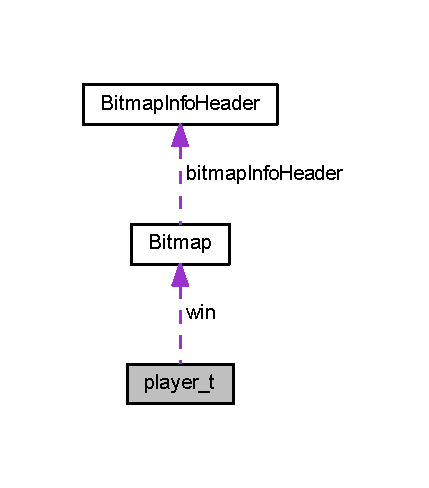
\includegraphics[width=206pt]{structplayer__t__coll__graph}
\end{center}
\end{figure}
\subsection*{Data Fields}
\begin{DoxyCompactItemize}
\item 
unsigned int \hyperlink{group___game_ga676e0da0ef83bbbdf42538e54b97506b}{x}
\item 
unsigned int \hyperlink{group___game_gac30de26db5f6d1c18c63913729adca7d}{y}
\item 
\hyperlink{group___game_gaa0aafed44fec19806d8f9ad834be1248}{state\+\_\+t} \hyperlink{group___game_ga9a379079ab305d43e4c73334578f9325}{st}
\item 
unsigned int \hyperlink{group___game_ga6325f05cd0c308b41c677ec0709707a4}{lost}
\item 
unsigned long \hyperlink{group___game_gab817949ca924898b4cc07f87e9936c37}{color1}
\item 
unsigned long \hyperlink{group___game_gad66b83194e360e19ab982ad5e92c0e47}{color2}
\item 
unsigned long \hyperlink{group___game_ga4a11e85efa70b04b658bbb13b38331a6}{color3}
\item 
unsigned long \hyperlink{group___game_ga74dc52caaf927df421fcbda624d6db30}{left}
\item 
unsigned long \hyperlink{group___game_gad9567130205b4716d5412d5d936cdeb0}{right}
\item 
\hyperlink{struct_bitmap}{Bitmap} $\ast$ \hyperlink{group___game_ga710a78637db874c6ee469e4a3f339f7f}{win}
\end{DoxyCompactItemize}


The documentation for this struct was generated from the following file\+:\begin{DoxyCompactItemize}
\item 
C\+:/\+Users/jnuno/\+Desktop/src/\hyperlink{tools_8h}{tools.\+h}\end{DoxyCompactItemize}

\chapter{File Documentation}
\hypertarget{game_8c}{}\section{C\+:/\+Users/jnuno/\+Desktop/src/game.c File Reference}
\label{game_8c}\index{C\+:/\+Users/jnuno/\+Desktop/src/game.\+c@{C\+:/\+Users/jnuno/\+Desktop/src/game.\+c}}
{\ttfamily \#include $<$minix/syslib.\+h$>$}\newline
{\ttfamily \#include $<$minix/drivers.\+h$>$}\newline
{\ttfamily \#include $<$machine/int86.\+h$>$}\newline
{\ttfamily \#include $<$sys/mman.\+h$>$}\newline
{\ttfamily \#include $<$sys/types.\+h$>$}\newline
{\ttfamily \#include \char`\"{}game.\+h\char`\"{}}\newline
{\ttfamily \#include \char`\"{}video\+\_\+gr.\+h\char`\"{}}\newline
{\ttfamily \#include \char`\"{}otherlabs.\+h\char`\"{}}\newline
{\ttfamily \#include \char`\"{}read\+\_\+bitmap.\+h\char`\"{}}\newline
{\ttfamily \#include \char`\"{}tools.\+h\char`\"{}}\newline
Include dependency graph for game.\+c\+:
\nopagebreak
\begin{figure}[H]
\begin{center}
\leavevmode
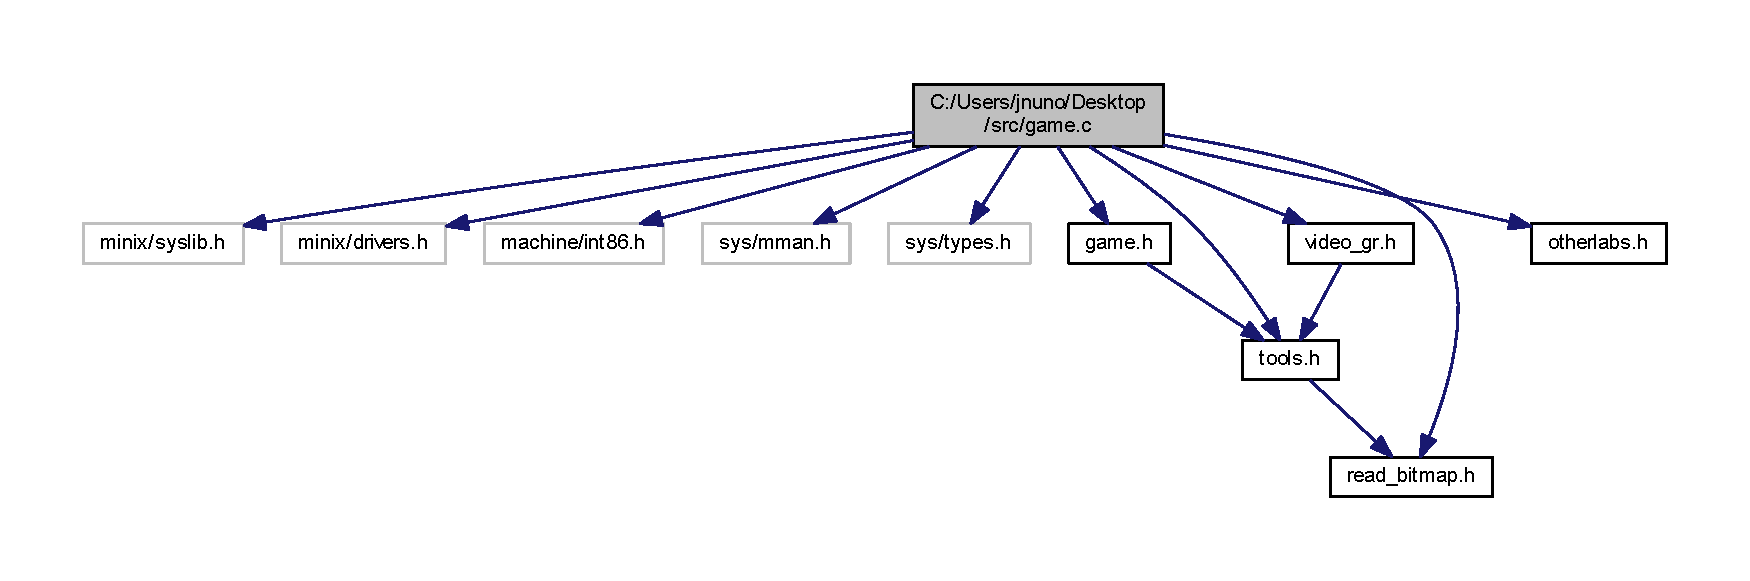
\includegraphics[width=350pt]{game_8c__incl}
\end{center}
\end{figure}
\subsection*{Functions}
\begin{DoxyCompactItemize}
\item 
void \hyperlink{game_8c_a2d7ae67897b06ba4d723f059b8055c3d}{load\+\_\+\+Bmps} (\hyperlink{structgame__t}{game\+\_\+t} $\ast$game1)
\begin{DoxyCompactList}\small\item\em Loads all Bitmaps needed in the Game. \end{DoxyCompactList}\item 
void \hyperlink{game_8c_a21785a858236fb7d375400e0e338336d}{change\+\_\+plst\+\_\+handler} (unsigned int num\+\_\+players, unsigned long data, \hyperlink{structgame__t}{game\+\_\+t} $\ast$game1)
\begin{DoxyCompactList}\small\item\em Handler for Player States. \end{DoxyCompactList}\item 
void \hyperlink{game_8c_af630a71e15386edfe50f4f8a303d9c39}{change\+\_\+player\+\_\+state} (\hyperlink{structplayer__t}{player\+\_\+t} $\ast$p, unsigned long data)
\begin{DoxyCompactList}\small\item\em Changes the movement state accordingly with the Data. \end{DoxyCompactList}\item 
void \hyperlink{game_8c_ab3383bfc12cb6695ede9ecd5f6573676}{update\+\_\+player} (unsigned int num\+\_\+players, \hyperlink{structgame__t}{game\+\_\+t} $\ast$game1)
\begin{DoxyCompactList}\small\item\em Updates the position of a Player based on its movement. \end{DoxyCompactList}\item 
void \hyperlink{game_8c_a89d72a2401cc9faf9102dbe393dee79a}{draw\+\_\+handler} (unsigned int num\+\_\+players, \hyperlink{structgame__t}{game\+\_\+t} $\ast$game1)
\begin{DoxyCompactList}\small\item\em Handler for Painting the Players. \end{DoxyCompactList}\item 
void \hyperlink{game_8c_a505eb2e66f358efafd4f23bca70cfa14}{state\+\_\+handler} (unsigned int num\+\_\+players, unsigned long data, \hyperlink{structgame__t}{game\+\_\+t} $\ast$game1)
\begin{DoxyCompactList}\small\item\em Handler for Game States. \end{DoxyCompactList}\item 
int \hyperlink{game_8c_a01f0539de201b53e0e5adb9d985327ff}{check\+\_\+mouse} (\hyperlink{structgame__t}{game\+\_\+t} $\ast$game1)
\begin{DoxyCompactList}\small\item\em Checks if Mouse is inside a Button in Menu. \end{DoxyCompactList}\item 
int \hyperlink{game_8c_acde10310f33cafd602e547fdcc87e5f7}{mouse\+\_\+mov\+\_\+handler} (unsigned long mouse\+\_\+packet\mbox{[}3\mbox{]}, \hyperlink{structgame__t}{game\+\_\+t} $\ast$game1)
\begin{DoxyCompactList}\small\item\em Mouse Handler for Menu. \end{DoxyCompactList}\item 
void \hyperlink{game_8c_a5745594a9d371072ebddb008b3b08699}{mouse\+\_\+st\+\_\+handler} (\hyperlink{structplayer__t}{player\+\_\+t} $\ast$p, unsigned long mouse\+\_\+packet\mbox{[}3\mbox{]}, \hyperlink{structgame__t}{game\+\_\+t} $\ast$game1)
\begin{DoxyCompactList}\small\item\em Mouse State Handler for Player 4. \end{DoxyCompactList}\item 
void \hyperlink{game_8c_ad1f78202a4ea7e8e68ba069a82484592}{check\+\_\+winner} (\hyperlink{structgame__t}{game\+\_\+t} $\ast$game1)
\begin{DoxyCompactList}\small\item\em Checks who wins and displays the winner bitmap. \end{DoxyCompactList}\item 
void \hyperlink{game_8c_a86358e01f0d51114bc31ea1b623ee024}{timer\+\_\+intrhandler} (\hyperlink{structgame__t}{game\+\_\+t} $\ast$game1)
\begin{DoxyCompactList}\small\item\em Handler for Timer Interrupts. \end{DoxyCompactList}\item 
void \hyperlink{game_8c_ac1990a9d59c2e1b744129d6990733f65}{kbd\+\_\+intrhandler} (unsigned long datakbd, \hyperlink{structgame__t}{game\+\_\+t} $\ast$game1)
\begin{DoxyCompactList}\small\item\em Handler for Keyboard Interrupts. \end{DoxyCompactList}\item 
void \hyperlink{game_8c_a7485cadb508c6cbe1efe9d01643b34e0}{mouse\+\_\+intrhandler} (unsigned long mouse\+\_\+packet\mbox{[}3\mbox{]}, \hyperlink{structgame__t}{game\+\_\+t} $\ast$game1)
\begin{DoxyCompactList}\small\item\em Handler for Mouse Interrupts. \end{DoxyCompactList}\item 
int \hyperlink{game_8c_afdeb92b797c5bbc22fa9cea605f6644b}{playgame} (\hyperlink{structgame__t}{game\+\_\+t} $\ast$game1)
\begin{DoxyCompactList}\small\item\em The Game Function. \end{DoxyCompactList}\item 
int \hyperlink{game_8c_a59430d80f49694010887ac3ab116e696}{start\+\_\+multigame} (unsigned int num\+\_\+players, \hyperlink{structgame__t}{game\+\_\+t} $\ast$game1)
\begin{DoxyCompactList}\small\item\em Starts a Multiplayer Game accorgingly to the Number of Players. \end{DoxyCompactList}\end{DoxyCompactItemize}


\subsection{Function Documentation}
\hypertarget{game_8c_af630a71e15386edfe50f4f8a303d9c39}{}\label{game_8c_af630a71e15386edfe50f4f8a303d9c39} 
\index{game.\+c@{game.\+c}!change\+\_\+player\+\_\+state@{change\+\_\+player\+\_\+state}}
\index{change\+\_\+player\+\_\+state@{change\+\_\+player\+\_\+state}!game.\+c@{game.\+c}}
\subsubsection{\texorpdfstring{change\+\_\+player\+\_\+state()}{change\_player\_state()}}
{\footnotesize\ttfamily void change\+\_\+player\+\_\+state (\begin{DoxyParamCaption}\item[{\hyperlink{structplayer__t}{player\+\_\+t} $\ast$}]{p,  }\item[{unsigned long}]{data }\end{DoxyParamCaption})}



Changes the movement state accordingly with the Data. 


\begin{DoxyParams}{Parameters}
{\em $\ast$p} & Player \\
\hline
{\em data} & Keyboard data \\
\hline
\end{DoxyParams}
\hypertarget{game_8c_a21785a858236fb7d375400e0e338336d}{}\label{game_8c_a21785a858236fb7d375400e0e338336d} 
\index{game.\+c@{game.\+c}!change\+\_\+plst\+\_\+handler@{change\+\_\+plst\+\_\+handler}}
\index{change\+\_\+plst\+\_\+handler@{change\+\_\+plst\+\_\+handler}!game.\+c@{game.\+c}}
\subsubsection{\texorpdfstring{change\+\_\+plst\+\_\+handler()}{change\_plst\_handler()}}
{\footnotesize\ttfamily void change\+\_\+plst\+\_\+handler (\begin{DoxyParamCaption}\item[{unsigned int}]{num\+\_\+players,  }\item[{unsigned long}]{data,  }\item[{\hyperlink{structgame__t}{game\+\_\+t} $\ast$}]{game1 }\end{DoxyParamCaption})}



Handler for Player States. 

Calls the other function accordingly to the Number of Players


\begin{DoxyParams}{Parameters}
{\em num\+\_\+players} & Number of Players in the current Game Mode \\
\hline
{\em data} & Keyboard data \\
\hline
{\em $\ast$game1} & The game itself \\
\hline
\end{DoxyParams}
Here is the call graph for this function\+:
\nopagebreak
\begin{figure}[H]
\begin{center}
\leavevmode
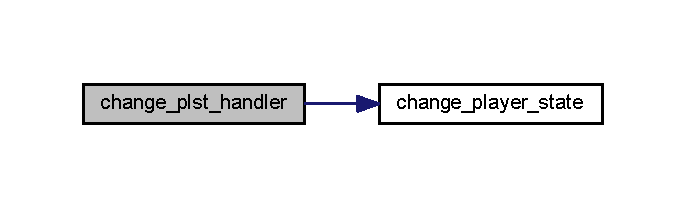
\includegraphics[width=329pt]{game_8c_a21785a858236fb7d375400e0e338336d_cgraph}
\end{center}
\end{figure}
\hypertarget{game_8c_a01f0539de201b53e0e5adb9d985327ff}{}\label{game_8c_a01f0539de201b53e0e5adb9d985327ff} 
\index{game.\+c@{game.\+c}!check\+\_\+mouse@{check\+\_\+mouse}}
\index{check\+\_\+mouse@{check\+\_\+mouse}!game.\+c@{game.\+c}}
\subsubsection{\texorpdfstring{check\+\_\+mouse()}{check\_mouse()}}
{\footnotesize\ttfamily int check\+\_\+mouse (\begin{DoxyParamCaption}\item[{\hyperlink{structgame__t}{game\+\_\+t} $\ast$}]{game1 }\end{DoxyParamCaption})}



Checks if Mouse is inside a Button in Menu. 


\begin{DoxyParams}{Parameters}
{\em $\ast$game1} & The game itself \\
\hline
\end{DoxyParams}
\begin{DoxyReturn}{Returns}
Return 0 if not in a buttton and non-\/zero otherwise 
\end{DoxyReturn}
\hypertarget{game_8c_ad1f78202a4ea7e8e68ba069a82484592}{}\label{game_8c_ad1f78202a4ea7e8e68ba069a82484592} 
\index{game.\+c@{game.\+c}!check\+\_\+winner@{check\+\_\+winner}}
\index{check\+\_\+winner@{check\+\_\+winner}!game.\+c@{game.\+c}}
\subsubsection{\texorpdfstring{check\+\_\+winner()}{check\_winner()}}
{\footnotesize\ttfamily void check\+\_\+winner (\begin{DoxyParamCaption}\item[{\hyperlink{structgame__t}{game\+\_\+t} $\ast$}]{game1 }\end{DoxyParamCaption})}



Checks who wins and displays the winner bitmap. 


\begin{DoxyParams}{Parameters}
{\em $\ast$game1} & The game itself \\
\hline
\end{DoxyParams}
Here is the call graph for this function\+:
\nopagebreak
\begin{figure}[H]
\begin{center}
\leavevmode
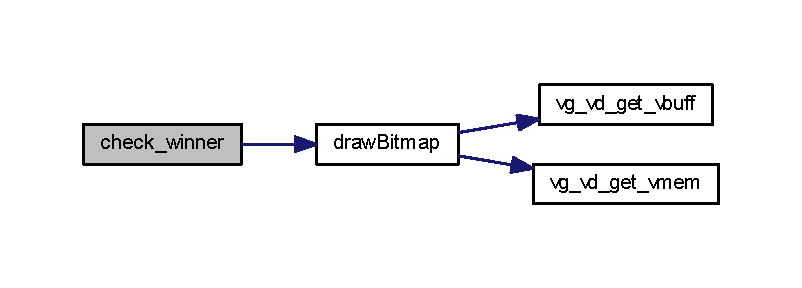
\includegraphics[width=350pt]{game_8c_ad1f78202a4ea7e8e68ba069a82484592_cgraph}
\end{center}
\end{figure}
\hypertarget{game_8c_a89d72a2401cc9faf9102dbe393dee79a}{}\label{game_8c_a89d72a2401cc9faf9102dbe393dee79a} 
\index{game.\+c@{game.\+c}!draw\+\_\+handler@{draw\+\_\+handler}}
\index{draw\+\_\+handler@{draw\+\_\+handler}!game.\+c@{game.\+c}}
\subsubsection{\texorpdfstring{draw\+\_\+handler()}{draw\_handler()}}
{\footnotesize\ttfamily void draw\+\_\+handler (\begin{DoxyParamCaption}\item[{unsigned int}]{num\+\_\+players,  }\item[{\hyperlink{structgame__t}{game\+\_\+t} $\ast$}]{game1 }\end{DoxyParamCaption})}



Handler for Painting the Players. 

Calls the other function accordingly to the Number of Players and if they didn\textquotesingle{}t already lost


\begin{DoxyParams}{Parameters}
{\em num\+\_\+players} & Number of Players in the current Game Mode \\
\hline
{\em $\ast$game1} & The game itself \\
\hline
\end{DoxyParams}
Here is the call graph for this function\+:
\nopagebreak
\begin{figure}[H]
\begin{center}
\leavevmode
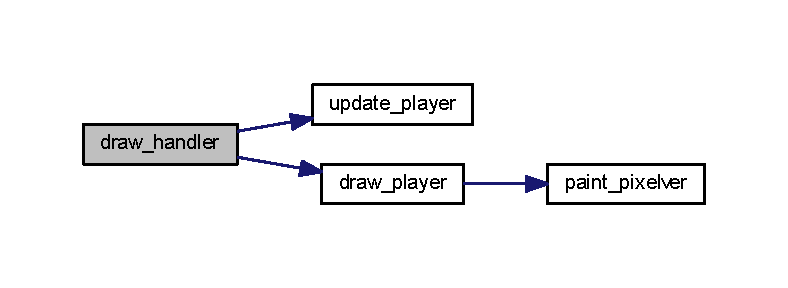
\includegraphics[width=350pt]{game_8c_a89d72a2401cc9faf9102dbe393dee79a_cgraph}
\end{center}
\end{figure}
\hypertarget{game_8c_ac1990a9d59c2e1b744129d6990733f65}{}\label{game_8c_ac1990a9d59c2e1b744129d6990733f65} 
\index{game.\+c@{game.\+c}!kbd\+\_\+intrhandler@{kbd\+\_\+intrhandler}}
\index{kbd\+\_\+intrhandler@{kbd\+\_\+intrhandler}!game.\+c@{game.\+c}}
\subsubsection{\texorpdfstring{kbd\+\_\+intrhandler()}{kbd\_intrhandler()}}
{\footnotesize\ttfamily void kbd\+\_\+intrhandler (\begin{DoxyParamCaption}\item[{unsigned long}]{datakbd,  }\item[{\hyperlink{structgame__t}{game\+\_\+t} $\ast$}]{game1 }\end{DoxyParamCaption})}



Handler for Keyboard Interrupts. 


\begin{DoxyParams}{Parameters}
{\em datakbd} & Keyboard Data \\
\hline
{\em $\ast$game1} & The game itself \\
\hline
\end{DoxyParams}
Here is the call graph for this function\+:
\nopagebreak
\begin{figure}[H]
\begin{center}
\leavevmode
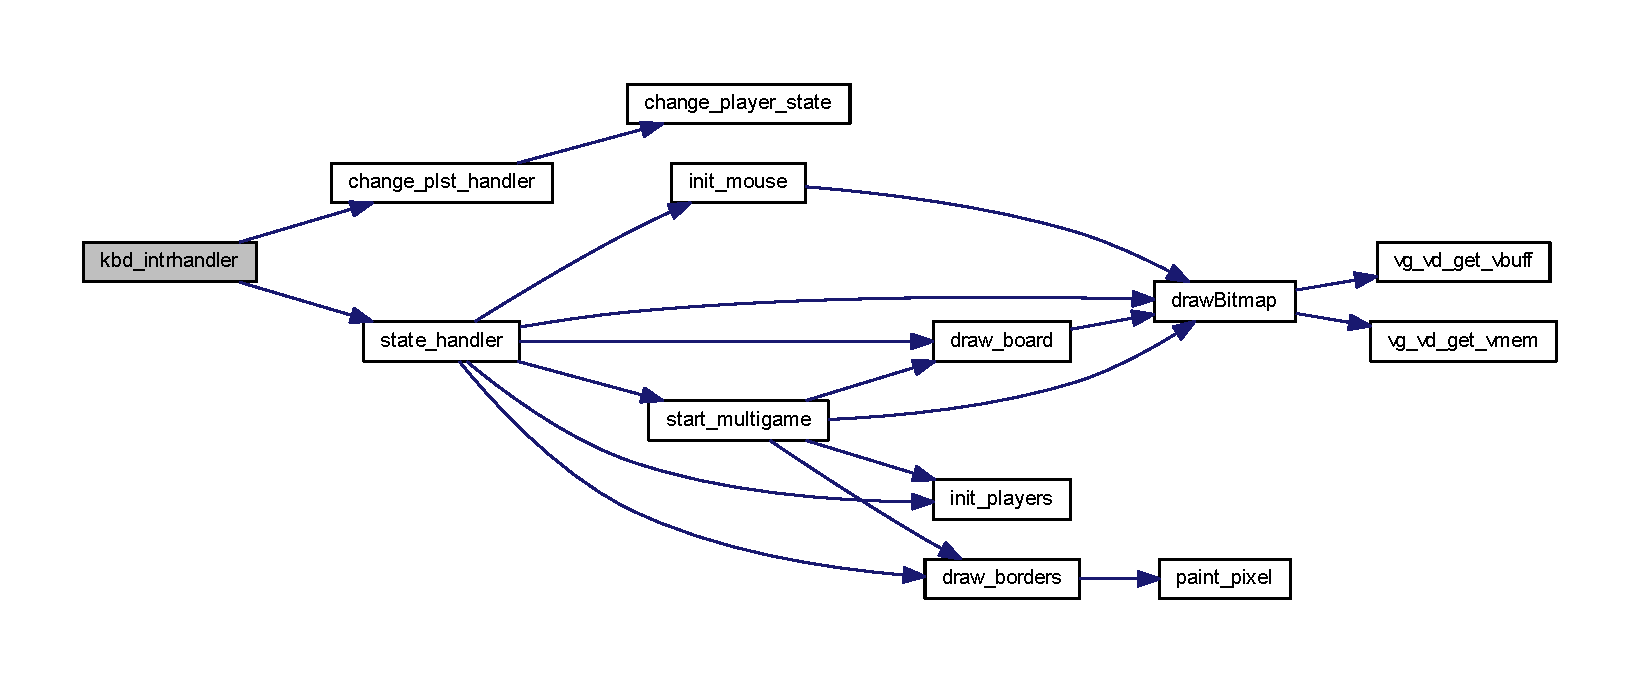
\includegraphics[width=350pt]{game_8c_ac1990a9d59c2e1b744129d6990733f65_cgraph}
\end{center}
\end{figure}
\hypertarget{game_8c_a2d7ae67897b06ba4d723f059b8055c3d}{}\label{game_8c_a2d7ae67897b06ba4d723f059b8055c3d} 
\index{game.\+c@{game.\+c}!load\+\_\+\+Bmps@{load\+\_\+\+Bmps}}
\index{load\+\_\+\+Bmps@{load\+\_\+\+Bmps}!game.\+c@{game.\+c}}
\subsubsection{\texorpdfstring{load\+\_\+\+Bmps()}{load\_Bmps()}}
{\footnotesize\ttfamily void load\+\_\+\+Bmps (\begin{DoxyParamCaption}\item[{\hyperlink{structgame__t}{game\+\_\+t} $\ast$}]{game1 }\end{DoxyParamCaption})}



Loads all Bitmaps needed in the Game. 

Here is the call graph for this function\+:
\nopagebreak
\begin{figure}[H]
\begin{center}
\leavevmode
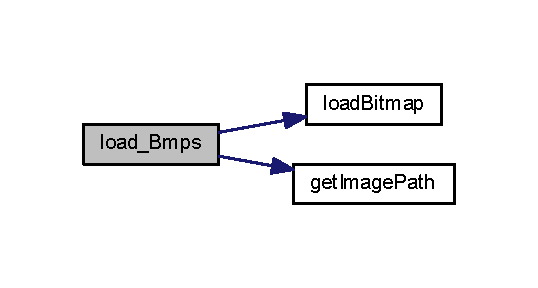
\includegraphics[width=258pt]{game_8c_a2d7ae67897b06ba4d723f059b8055c3d_cgraph}
\end{center}
\end{figure}
\hypertarget{game_8c_a7485cadb508c6cbe1efe9d01643b34e0}{}\label{game_8c_a7485cadb508c6cbe1efe9d01643b34e0} 
\index{game.\+c@{game.\+c}!mouse\+\_\+intrhandler@{mouse\+\_\+intrhandler}}
\index{mouse\+\_\+intrhandler@{mouse\+\_\+intrhandler}!game.\+c@{game.\+c}}
\subsubsection{\texorpdfstring{mouse\+\_\+intrhandler()}{mouse\_intrhandler()}}
{\footnotesize\ttfamily void mouse\+\_\+intrhandler (\begin{DoxyParamCaption}\item[{unsigned long}]{mouse\+\_\+packet\mbox{[}3\mbox{]},  }\item[{\hyperlink{structgame__t}{game\+\_\+t} $\ast$}]{game1 }\end{DoxyParamCaption})}



Handler for Mouse Interrupts. 


\begin{DoxyParams}{Parameters}
{\em mouse\+\_\+packet\mbox{[}3\mbox{]}} & Data packets of the Mouse \\
\hline
{\em $\ast$game1} & The game itself \\
\hline
\end{DoxyParams}
Here is the call graph for this function\+:
\nopagebreak
\begin{figure}[H]
\begin{center}
\leavevmode
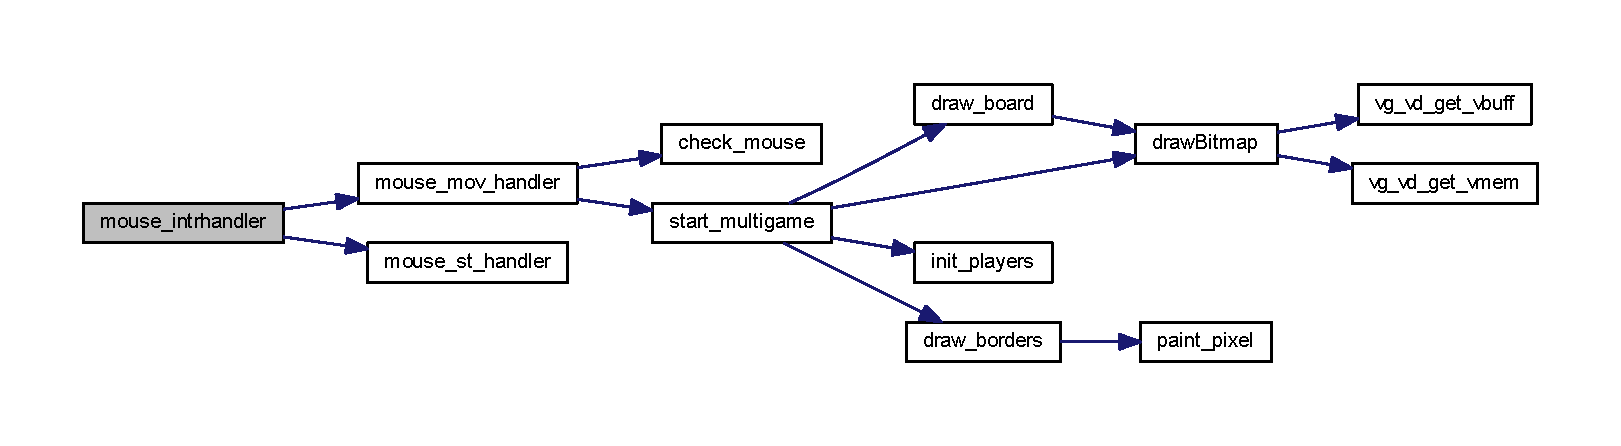
\includegraphics[width=350pt]{game_8c_a7485cadb508c6cbe1efe9d01643b34e0_cgraph}
\end{center}
\end{figure}
\hypertarget{game_8c_acde10310f33cafd602e547fdcc87e5f7}{}\label{game_8c_acde10310f33cafd602e547fdcc87e5f7} 
\index{game.\+c@{game.\+c}!mouse\+\_\+mov\+\_\+handler@{mouse\+\_\+mov\+\_\+handler}}
\index{mouse\+\_\+mov\+\_\+handler@{mouse\+\_\+mov\+\_\+handler}!game.\+c@{game.\+c}}
\subsubsection{\texorpdfstring{mouse\+\_\+mov\+\_\+handler()}{mouse\_mov\_handler()}}
{\footnotesize\ttfamily int mouse\+\_\+mov\+\_\+handler (\begin{DoxyParamCaption}\item[{unsigned long}]{mouse\+\_\+packet\mbox{[}3\mbox{]},  }\item[{\hyperlink{structgame__t}{game\+\_\+t} $\ast$}]{game1 }\end{DoxyParamCaption})}



Mouse Handler for Menu. 

Handles the buttons and movement of the mouse in the Menu


\begin{DoxyParams}{Parameters}
{\em mouse\+\_\+packet\mbox{[}3\mbox{]}} & Data packets of the Mouse \\
\hline
{\em $\ast$game1} & The game itself \\
\hline
\end{DoxyParams}
\begin{DoxyReturn}{Returns}
Return 1 on acceptable data and 0 if overflow 
\end{DoxyReturn}
Here is the call graph for this function\+:
\nopagebreak
\begin{figure}[H]
\begin{center}
\leavevmode
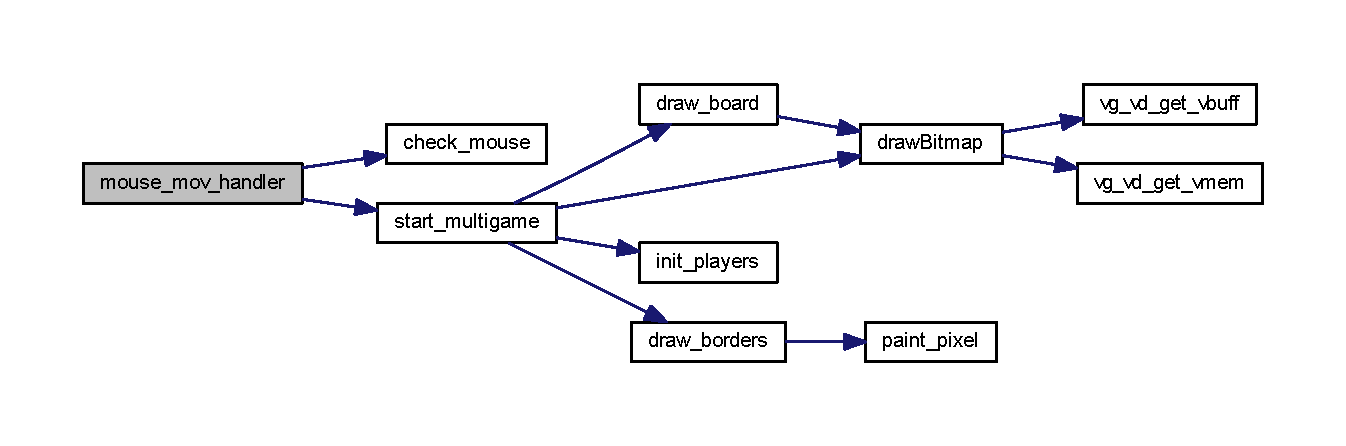
\includegraphics[width=350pt]{game_8c_acde10310f33cafd602e547fdcc87e5f7_cgraph}
\end{center}
\end{figure}
\hypertarget{game_8c_a5745594a9d371072ebddb008b3b08699}{}\label{game_8c_a5745594a9d371072ebddb008b3b08699} 
\index{game.\+c@{game.\+c}!mouse\+\_\+st\+\_\+handler@{mouse\+\_\+st\+\_\+handler}}
\index{mouse\+\_\+st\+\_\+handler@{mouse\+\_\+st\+\_\+handler}!game.\+c@{game.\+c}}
\subsubsection{\texorpdfstring{mouse\+\_\+st\+\_\+handler()}{mouse\_st\_handler()}}
{\footnotesize\ttfamily void mouse\+\_\+st\+\_\+handler (\begin{DoxyParamCaption}\item[{\hyperlink{structplayer__t}{player\+\_\+t} $\ast$}]{p,  }\item[{unsigned long}]{mouse\+\_\+packet\mbox{[}3\mbox{]},  }\item[{\hyperlink{structgame__t}{game\+\_\+t} $\ast$}]{game1 }\end{DoxyParamCaption})}



Mouse State Handler for Player 4. 


\begin{DoxyParams}{Parameters}
{\em $\ast$p} & Player \\
\hline
{\em mouse\+\_\+packet\mbox{[}3\mbox{]}} & Data packets of the Mouse \\
\hline
{\em $\ast$game1} & The game itself \\
\hline
\end{DoxyParams}
\hypertarget{game_8c_afdeb92b797c5bbc22fa9cea605f6644b}{}\label{game_8c_afdeb92b797c5bbc22fa9cea605f6644b} 
\index{game.\+c@{game.\+c}!playgame@{playgame}}
\index{playgame@{playgame}!game.\+c@{game.\+c}}
\subsubsection{\texorpdfstring{playgame()}{playgame()}}
{\footnotesize\ttfamily int playgame (\begin{DoxyParamCaption}\item[{\hyperlink{structgame__t}{game\+\_\+t} $\ast$}]{game1 }\end{DoxyParamCaption})}



The Game Function. 

Interrupts cycle


\begin{DoxyParams}{Parameters}
{\em $\ast$game1} & The game itself \\
\hline
\end{DoxyParams}
Here is the call graph for this function\+:
\nopagebreak
\begin{figure}[H]
\begin{center}
\leavevmode
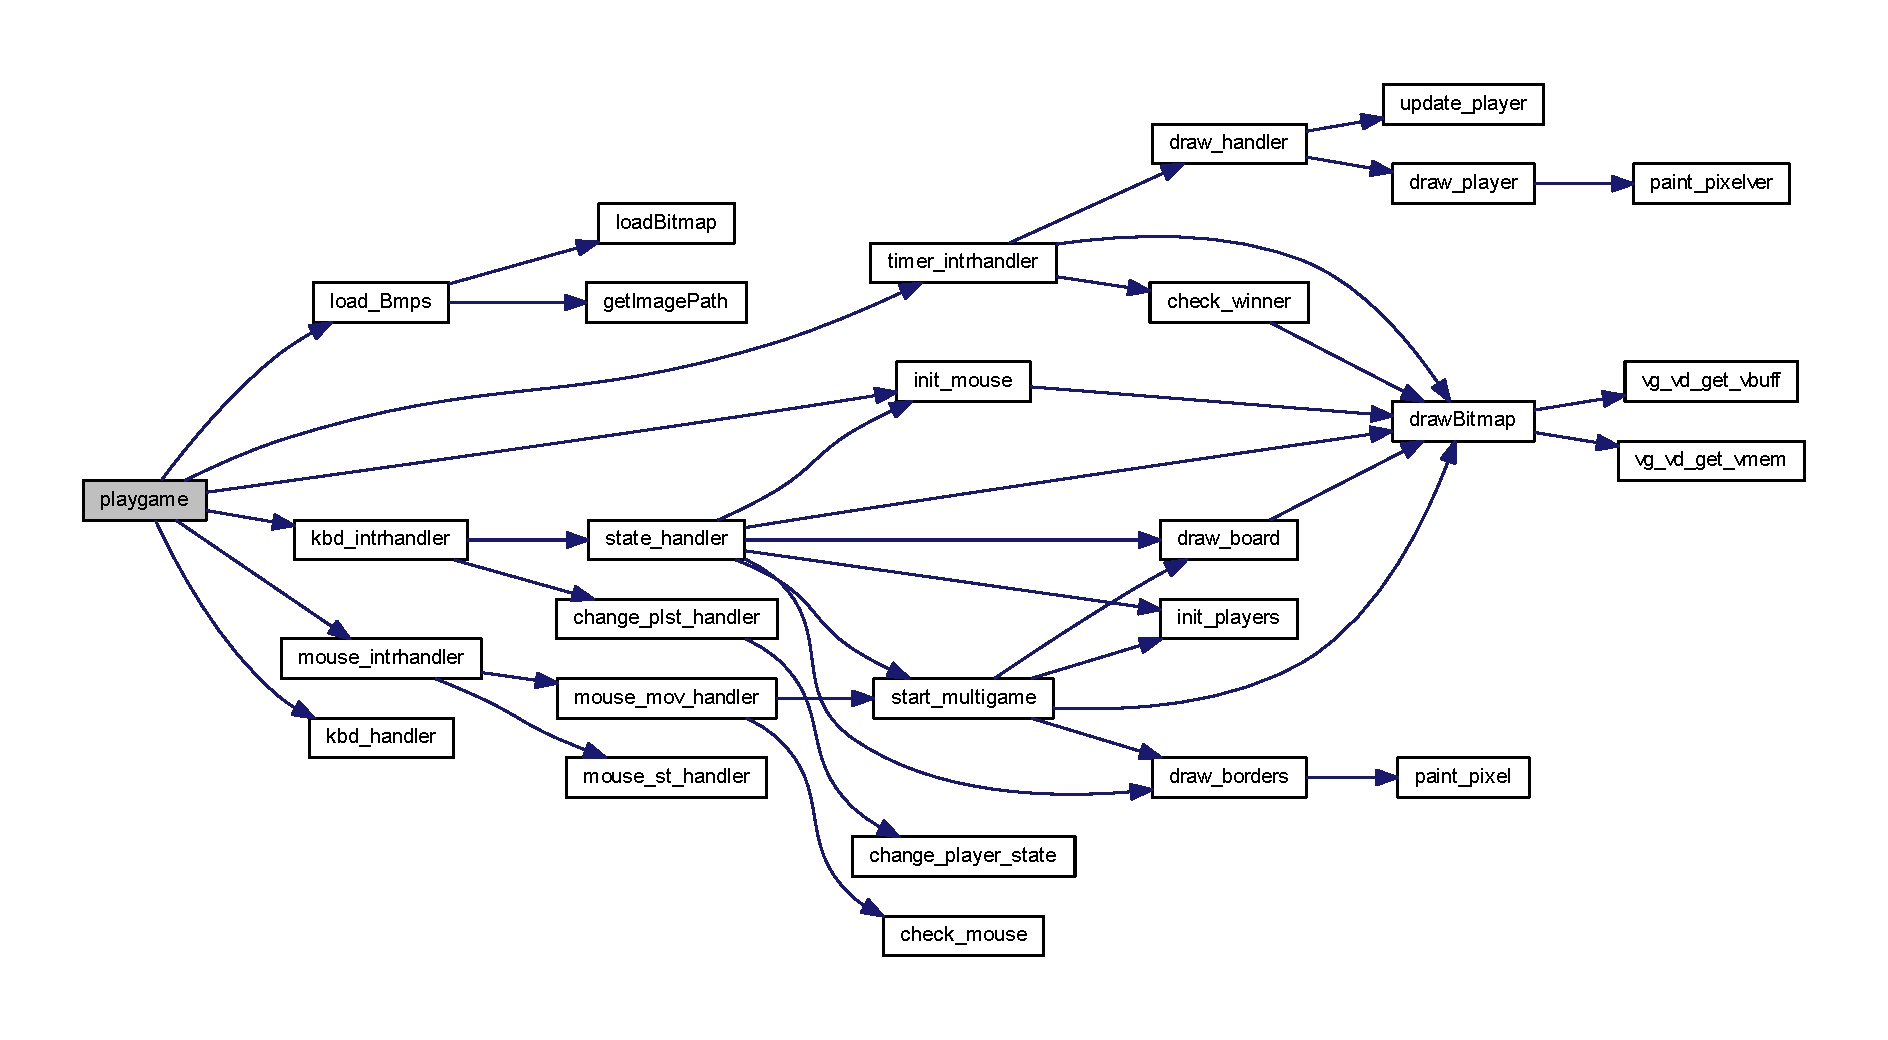
\includegraphics[width=350pt]{game_8c_afdeb92b797c5bbc22fa9cea605f6644b_cgraph}
\end{center}
\end{figure}
\hypertarget{game_8c_a59430d80f49694010887ac3ab116e696}{}\label{game_8c_a59430d80f49694010887ac3ab116e696} 
\index{game.\+c@{game.\+c}!start\+\_\+multigame@{start\+\_\+multigame}}
\index{start\+\_\+multigame@{start\+\_\+multigame}!game.\+c@{game.\+c}}
\subsubsection{\texorpdfstring{start\+\_\+multigame()}{start\_multigame()}}
{\footnotesize\ttfamily int start\+\_\+multigame (\begin{DoxyParamCaption}\item[{unsigned int}]{num\+\_\+players,  }\item[{\hyperlink{structgame__t}{game\+\_\+t} $\ast$}]{game1 }\end{DoxyParamCaption})}



Starts a Multiplayer Game accorgingly to the Number of Players. 


\begin{DoxyParams}{Parameters}
{\em num\+\_\+players} & Number of Players on the Game Mode \\
\hline
{\em $\ast$game1} & The game itself \\
\hline
\end{DoxyParams}
\begin{DoxyReturn}{Returns}
Return 0 on success and 1 otherwise 
\end{DoxyReturn}
Here is the call graph for this function\+:
\nopagebreak
\begin{figure}[H]
\begin{center}
\leavevmode
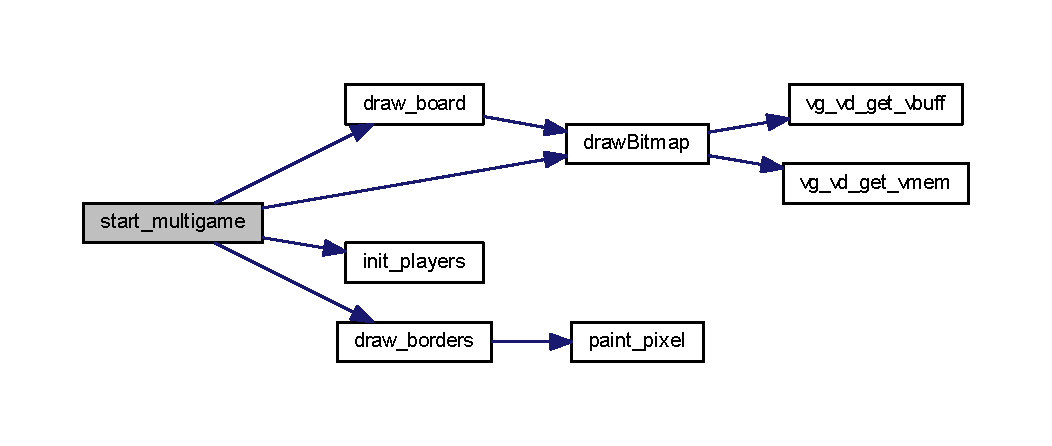
\includegraphics[width=350pt]{game_8c_a59430d80f49694010887ac3ab116e696_cgraph}
\end{center}
\end{figure}
\hypertarget{game_8c_a505eb2e66f358efafd4f23bca70cfa14}{}\label{game_8c_a505eb2e66f358efafd4f23bca70cfa14} 
\index{game.\+c@{game.\+c}!state\+\_\+handler@{state\+\_\+handler}}
\index{state\+\_\+handler@{state\+\_\+handler}!game.\+c@{game.\+c}}
\subsubsection{\texorpdfstring{state\+\_\+handler()}{state\_handler()}}
{\footnotesize\ttfamily void state\+\_\+handler (\begin{DoxyParamCaption}\item[{unsigned int}]{num\+\_\+players,  }\item[{unsigned long}]{data,  }\item[{\hyperlink{structgame__t}{game\+\_\+t} $\ast$}]{game1 }\end{DoxyParamCaption})}



Handler for Game States. 


\begin{DoxyParams}{Parameters}
{\em num\+\_\+players} & Number of Players in the current Game Mode \\
\hline
{\em data} & Keyboard data \\
\hline
{\em $\ast$game1} & The game itself \\
\hline
\end{DoxyParams}
Here is the call graph for this function\+:
\nopagebreak
\begin{figure}[H]
\begin{center}
\leavevmode
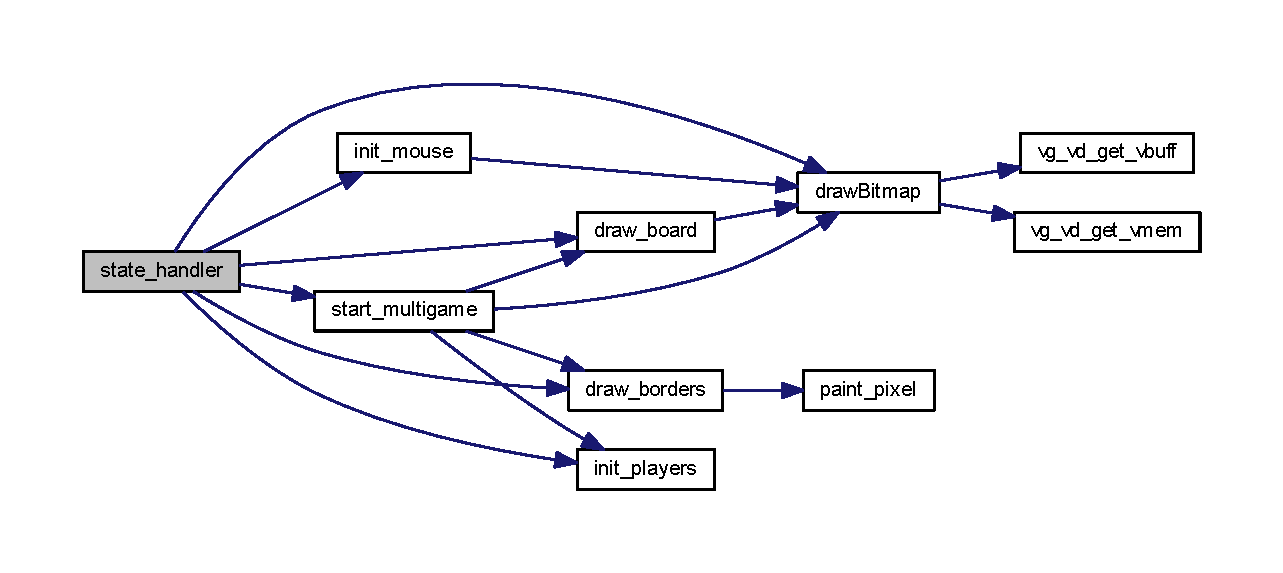
\includegraphics[width=350pt]{game_8c_a505eb2e66f358efafd4f23bca70cfa14_cgraph}
\end{center}
\end{figure}
\hypertarget{game_8c_a86358e01f0d51114bc31ea1b623ee024}{}\label{game_8c_a86358e01f0d51114bc31ea1b623ee024} 
\index{game.\+c@{game.\+c}!timer\+\_\+intrhandler@{timer\+\_\+intrhandler}}
\index{timer\+\_\+intrhandler@{timer\+\_\+intrhandler}!game.\+c@{game.\+c}}
\subsubsection{\texorpdfstring{timer\+\_\+intrhandler()}{timer\_intrhandler()}}
{\footnotesize\ttfamily void timer\+\_\+intrhandler (\begin{DoxyParamCaption}\item[{\hyperlink{structgame__t}{game\+\_\+t} $\ast$}]{game1 }\end{DoxyParamCaption})}



Handler for Timer Interrupts. 


\begin{DoxyParams}{Parameters}
{\em $\ast$game1} & The game itself \\
\hline
\end{DoxyParams}
Here is the call graph for this function\+:
\nopagebreak
\begin{figure}[H]
\begin{center}
\leavevmode
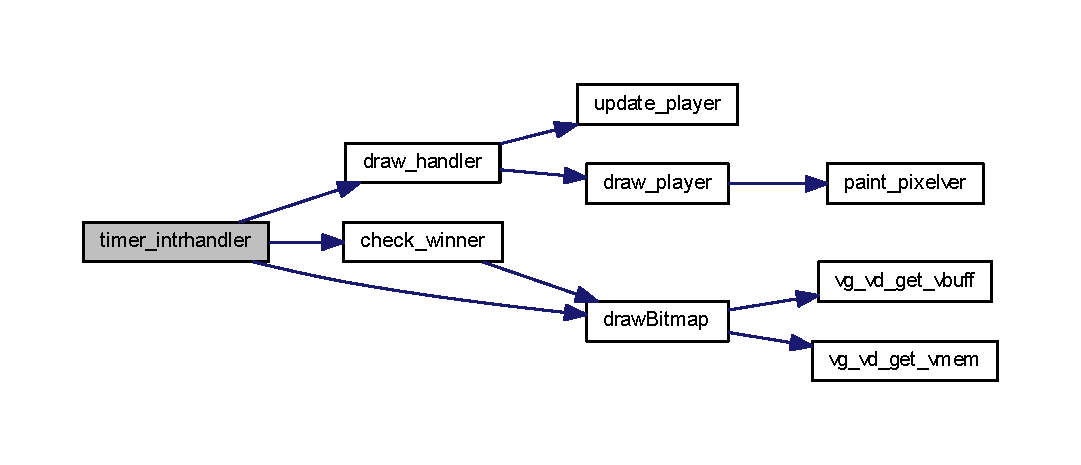
\includegraphics[width=350pt]{game_8c_a86358e01f0d51114bc31ea1b623ee024_cgraph}
\end{center}
\end{figure}
\hypertarget{game_8c_ab3383bfc12cb6695ede9ecd5f6573676}{}\label{game_8c_ab3383bfc12cb6695ede9ecd5f6573676} 
\index{game.\+c@{game.\+c}!update\+\_\+player@{update\+\_\+player}}
\index{update\+\_\+player@{update\+\_\+player}!game.\+c@{game.\+c}}
\subsubsection{\texorpdfstring{update\+\_\+player()}{update\_player()}}
{\footnotesize\ttfamily void update\+\_\+player (\begin{DoxyParamCaption}\item[{unsigned int}]{num\+\_\+players,  }\item[{\hyperlink{structgame__t}{game\+\_\+t} $\ast$}]{game1 }\end{DoxyParamCaption})}



Updates the position of a Player based on its movement. 


\begin{DoxyParams}{Parameters}
{\em num\+\_\+players} & Number of Players in the current Game Mode \\
\hline
{\em $\ast$game1} & The game itself \\
\hline
\end{DoxyParams}

\hypertarget{game_8h}{}\section{C\+:/\+Users/jnuno/\+Desktop/src/game.h File Reference}
\label{game_8h}\index{C\+:/\+Users/jnuno/\+Desktop/src/game.\+h@{C\+:/\+Users/jnuno/\+Desktop/src/game.\+h}}
{\ttfamily \#include \char`\"{}tools.\+h\char`\"{}}\newline
Include dependency graph for game.\+h\+:
\nopagebreak
\begin{figure}[H]
\begin{center}
\leavevmode
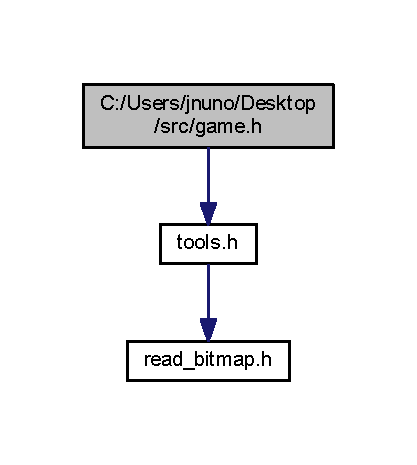
\includegraphics[width=200pt]{game_8h__incl}
\end{center}
\end{figure}
This graph shows which files directly or indirectly include this file\+:
\nopagebreak
\begin{figure}[H]
\begin{center}
\leavevmode
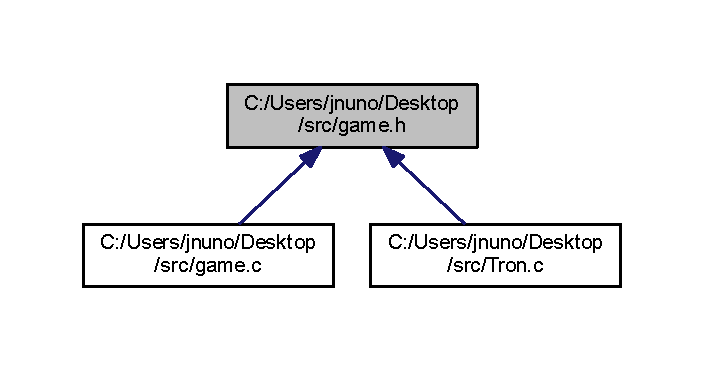
\includegraphics[width=338pt]{game_8h__dep__incl}
\end{center}
\end{figure}
\subsection*{Functions}
\begin{DoxyCompactItemize}
\item 
void \hyperlink{game_8h_a2d7ae67897b06ba4d723f059b8055c3d}{load\+\_\+\+Bmps} (\hyperlink{structgame__t}{game\+\_\+t} $\ast$game1)
\begin{DoxyCompactList}\small\item\em Loads all Bitmaps needed in the Game. \end{DoxyCompactList}\item 
void \hyperlink{game_8h_a21785a858236fb7d375400e0e338336d}{change\+\_\+plst\+\_\+handler} (unsigned int num\+\_\+players, unsigned long data, \hyperlink{structgame__t}{game\+\_\+t} $\ast$game1)
\begin{DoxyCompactList}\small\item\em Handler for Player States. \end{DoxyCompactList}\item 
void \hyperlink{game_8h_af630a71e15386edfe50f4f8a303d9c39}{change\+\_\+player\+\_\+state} (\hyperlink{structplayer__t}{player\+\_\+t} $\ast$p, unsigned long data)
\begin{DoxyCompactList}\small\item\em Changes the movement state accordingly with the Data. \end{DoxyCompactList}\item 
void \hyperlink{game_8h_ab3383bfc12cb6695ede9ecd5f6573676}{update\+\_\+player} (unsigned int num\+\_\+players, \hyperlink{structgame__t}{game\+\_\+t} $\ast$game1)
\begin{DoxyCompactList}\small\item\em Updates the position of a Player based on its movement. \end{DoxyCompactList}\item 
void \hyperlink{game_8h_a89d72a2401cc9faf9102dbe393dee79a}{draw\+\_\+handler} (unsigned int num\+\_\+players, \hyperlink{structgame__t}{game\+\_\+t} $\ast$game1)
\begin{DoxyCompactList}\small\item\em Handler for Painting the Players. \end{DoxyCompactList}\item 
void \hyperlink{game_8h_a505eb2e66f358efafd4f23bca70cfa14}{state\+\_\+handler} (unsigned int num\+\_\+players, unsigned long data, \hyperlink{structgame__t}{game\+\_\+t} $\ast$game1)
\begin{DoxyCompactList}\small\item\em Handler for Game States. \end{DoxyCompactList}\item 
int \hyperlink{game_8h_a01f0539de201b53e0e5adb9d985327ff}{check\+\_\+mouse} (\hyperlink{structgame__t}{game\+\_\+t} $\ast$game1)
\begin{DoxyCompactList}\small\item\em Checks if Mouse is inside a Button in Menu. \end{DoxyCompactList}\item 
int \hyperlink{game_8h_acde10310f33cafd602e547fdcc87e5f7}{mouse\+\_\+mov\+\_\+handler} (unsigned long mouse\+\_\+packet\mbox{[}3\mbox{]}, \hyperlink{structgame__t}{game\+\_\+t} $\ast$game1)
\begin{DoxyCompactList}\small\item\em Mouse Handler for Menu. \end{DoxyCompactList}\item 
void \hyperlink{game_8h_a5745594a9d371072ebddb008b3b08699}{mouse\+\_\+st\+\_\+handler} (\hyperlink{structplayer__t}{player\+\_\+t} $\ast$p, unsigned long mouse\+\_\+packet\mbox{[}3\mbox{]}, \hyperlink{structgame__t}{game\+\_\+t} $\ast$game1)
\begin{DoxyCompactList}\small\item\em Mouse State Handler for Player 4. \end{DoxyCompactList}\item 
void \hyperlink{game_8h_ad1f78202a4ea7e8e68ba069a82484592}{check\+\_\+winner} (\hyperlink{structgame__t}{game\+\_\+t} $\ast$game1)
\begin{DoxyCompactList}\small\item\em Checks who wins and displays the winner bitmap. \end{DoxyCompactList}\item 
void \hyperlink{game_8h_a86358e01f0d51114bc31ea1b623ee024}{timer\+\_\+intrhandler} (\hyperlink{structgame__t}{game\+\_\+t} $\ast$game1)
\begin{DoxyCompactList}\small\item\em Handler for Timer Interrupts. \end{DoxyCompactList}\item 
void \hyperlink{game_8h_ac1990a9d59c2e1b744129d6990733f65}{kbd\+\_\+intrhandler} (unsigned long datakbd, \hyperlink{structgame__t}{game\+\_\+t} $\ast$game1)
\begin{DoxyCompactList}\small\item\em Handler for Keyboard Interrupts. \end{DoxyCompactList}\item 
void \hyperlink{game_8h_a7485cadb508c6cbe1efe9d01643b34e0}{mouse\+\_\+intrhandler} (unsigned long mouse\+\_\+packet\mbox{[}3\mbox{]}, \hyperlink{structgame__t}{game\+\_\+t} $\ast$game1)
\begin{DoxyCompactList}\small\item\em Handler for Mouse Interrupts. \end{DoxyCompactList}\item 
int \hyperlink{game_8h_afdeb92b797c5bbc22fa9cea605f6644b}{playgame} (\hyperlink{structgame__t}{game\+\_\+t} $\ast$game1)
\begin{DoxyCompactList}\small\item\em The Game Function. \end{DoxyCompactList}\item 
int \hyperlink{game_8h_a59430d80f49694010887ac3ab116e696}{start\+\_\+multigame} (unsigned int num\+\_\+players, \hyperlink{structgame__t}{game\+\_\+t} $\ast$game1)
\begin{DoxyCompactList}\small\item\em Starts a Multiplayer Game accorgingly to the Number of Players. \end{DoxyCompactList}\end{DoxyCompactItemize}


\subsection{Function Documentation}
\hypertarget{game_8h_af630a71e15386edfe50f4f8a303d9c39}{}\label{game_8h_af630a71e15386edfe50f4f8a303d9c39} 
\index{game.\+h@{game.\+h}!change\+\_\+player\+\_\+state@{change\+\_\+player\+\_\+state}}
\index{change\+\_\+player\+\_\+state@{change\+\_\+player\+\_\+state}!game.\+h@{game.\+h}}
\subsubsection{\texorpdfstring{change\+\_\+player\+\_\+state()}{change\_player\_state()}}
{\footnotesize\ttfamily void change\+\_\+player\+\_\+state (\begin{DoxyParamCaption}\item[{\hyperlink{structplayer__t}{player\+\_\+t} $\ast$}]{p,  }\item[{unsigned long}]{data }\end{DoxyParamCaption})}



Changes the movement state accordingly with the Data. 


\begin{DoxyParams}{Parameters}
{\em $\ast$p} & Player \\
\hline
{\em data} & Keyboard data \\
\hline
\end{DoxyParams}
\hypertarget{game_8h_a21785a858236fb7d375400e0e338336d}{}\label{game_8h_a21785a858236fb7d375400e0e338336d} 
\index{game.\+h@{game.\+h}!change\+\_\+plst\+\_\+handler@{change\+\_\+plst\+\_\+handler}}
\index{change\+\_\+plst\+\_\+handler@{change\+\_\+plst\+\_\+handler}!game.\+h@{game.\+h}}
\subsubsection{\texorpdfstring{change\+\_\+plst\+\_\+handler()}{change\_plst\_handler()}}
{\footnotesize\ttfamily void change\+\_\+plst\+\_\+handler (\begin{DoxyParamCaption}\item[{unsigned int}]{num\+\_\+players,  }\item[{unsigned long}]{data,  }\item[{\hyperlink{structgame__t}{game\+\_\+t} $\ast$}]{game1 }\end{DoxyParamCaption})}



Handler for Player States. 

Calls the other function accordingly to the Number of Players


\begin{DoxyParams}{Parameters}
{\em num\+\_\+players} & Number of Players in the current Game Mode \\
\hline
{\em data} & Keyboard data \\
\hline
{\em $\ast$game1} & The game itself \\
\hline
\end{DoxyParams}
Here is the call graph for this function\+:
\nopagebreak
\begin{figure}[H]
\begin{center}
\leavevmode
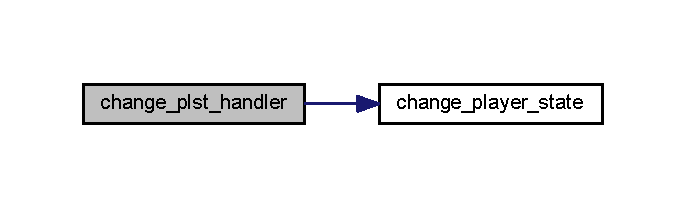
\includegraphics[width=329pt]{game_8h_a21785a858236fb7d375400e0e338336d_cgraph}
\end{center}
\end{figure}
\hypertarget{game_8h_a01f0539de201b53e0e5adb9d985327ff}{}\label{game_8h_a01f0539de201b53e0e5adb9d985327ff} 
\index{game.\+h@{game.\+h}!check\+\_\+mouse@{check\+\_\+mouse}}
\index{check\+\_\+mouse@{check\+\_\+mouse}!game.\+h@{game.\+h}}
\subsubsection{\texorpdfstring{check\+\_\+mouse()}{check\_mouse()}}
{\footnotesize\ttfamily int check\+\_\+mouse (\begin{DoxyParamCaption}\item[{\hyperlink{structgame__t}{game\+\_\+t} $\ast$}]{game1 }\end{DoxyParamCaption})}



Checks if Mouse is inside a Button in Menu. 


\begin{DoxyParams}{Parameters}
{\em $\ast$game1} & The game itself \\
\hline
\end{DoxyParams}
\begin{DoxyReturn}{Returns}
Return 0 if not in a buttton and non-\/zero otherwise 
\end{DoxyReturn}
\hypertarget{game_8h_ad1f78202a4ea7e8e68ba069a82484592}{}\label{game_8h_ad1f78202a4ea7e8e68ba069a82484592} 
\index{game.\+h@{game.\+h}!check\+\_\+winner@{check\+\_\+winner}}
\index{check\+\_\+winner@{check\+\_\+winner}!game.\+h@{game.\+h}}
\subsubsection{\texorpdfstring{check\+\_\+winner()}{check\_winner()}}
{\footnotesize\ttfamily void check\+\_\+winner (\begin{DoxyParamCaption}\item[{\hyperlink{structgame__t}{game\+\_\+t} $\ast$}]{game1 }\end{DoxyParamCaption})}



Checks who wins and displays the winner bitmap. 


\begin{DoxyParams}{Parameters}
{\em $\ast$game1} & The game itself \\
\hline
\end{DoxyParams}
Here is the call graph for this function\+:
\nopagebreak
\begin{figure}[H]
\begin{center}
\leavevmode
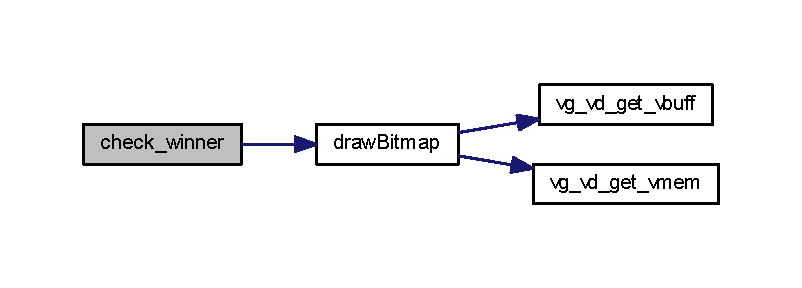
\includegraphics[width=350pt]{game_8h_ad1f78202a4ea7e8e68ba069a82484592_cgraph}
\end{center}
\end{figure}
\hypertarget{game_8h_a89d72a2401cc9faf9102dbe393dee79a}{}\label{game_8h_a89d72a2401cc9faf9102dbe393dee79a} 
\index{game.\+h@{game.\+h}!draw\+\_\+handler@{draw\+\_\+handler}}
\index{draw\+\_\+handler@{draw\+\_\+handler}!game.\+h@{game.\+h}}
\subsubsection{\texorpdfstring{draw\+\_\+handler()}{draw\_handler()}}
{\footnotesize\ttfamily void draw\+\_\+handler (\begin{DoxyParamCaption}\item[{unsigned int}]{num\+\_\+players,  }\item[{\hyperlink{structgame__t}{game\+\_\+t} $\ast$}]{game1 }\end{DoxyParamCaption})}



Handler for Painting the Players. 

Calls the other function accordingly to the Number of Players and if they didn\textquotesingle{}t already lost


\begin{DoxyParams}{Parameters}
{\em num\+\_\+players} & Number of Players in the current Game Mode \\
\hline
{\em $\ast$game1} & The game itself \\
\hline
\end{DoxyParams}
Here is the call graph for this function\+:
\nopagebreak
\begin{figure}[H]
\begin{center}
\leavevmode
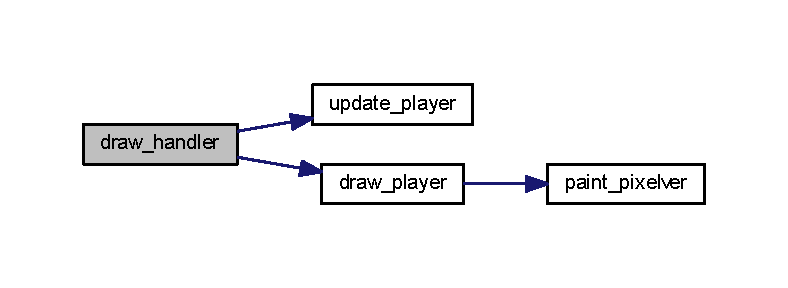
\includegraphics[width=350pt]{game_8h_a89d72a2401cc9faf9102dbe393dee79a_cgraph}
\end{center}
\end{figure}
\hypertarget{game_8h_ac1990a9d59c2e1b744129d6990733f65}{}\label{game_8h_ac1990a9d59c2e1b744129d6990733f65} 
\index{game.\+h@{game.\+h}!kbd\+\_\+intrhandler@{kbd\+\_\+intrhandler}}
\index{kbd\+\_\+intrhandler@{kbd\+\_\+intrhandler}!game.\+h@{game.\+h}}
\subsubsection{\texorpdfstring{kbd\+\_\+intrhandler()}{kbd\_intrhandler()}}
{\footnotesize\ttfamily void kbd\+\_\+intrhandler (\begin{DoxyParamCaption}\item[{unsigned long}]{datakbd,  }\item[{\hyperlink{structgame__t}{game\+\_\+t} $\ast$}]{game1 }\end{DoxyParamCaption})}



Handler for Keyboard Interrupts. 


\begin{DoxyParams}{Parameters}
{\em datakbd} & Keyboard Data \\
\hline
{\em $\ast$game1} & The game itself \\
\hline
\end{DoxyParams}
Here is the call graph for this function\+:
\nopagebreak
\begin{figure}[H]
\begin{center}
\leavevmode
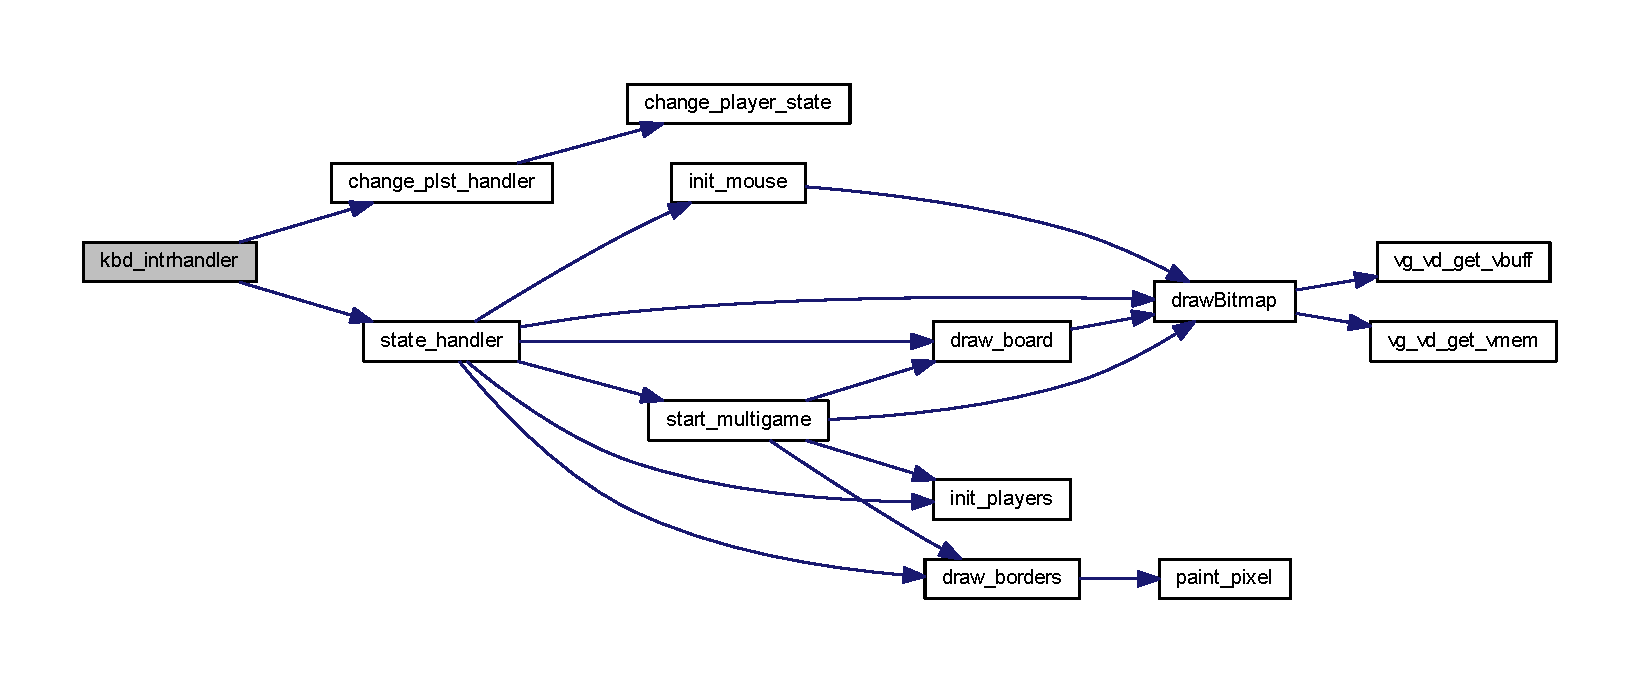
\includegraphics[width=350pt]{game_8h_ac1990a9d59c2e1b744129d6990733f65_cgraph}
\end{center}
\end{figure}
\hypertarget{game_8h_a2d7ae67897b06ba4d723f059b8055c3d}{}\label{game_8h_a2d7ae67897b06ba4d723f059b8055c3d} 
\index{game.\+h@{game.\+h}!load\+\_\+\+Bmps@{load\+\_\+\+Bmps}}
\index{load\+\_\+\+Bmps@{load\+\_\+\+Bmps}!game.\+h@{game.\+h}}
\subsubsection{\texorpdfstring{load\+\_\+\+Bmps()}{load\_Bmps()}}
{\footnotesize\ttfamily void load\+\_\+\+Bmps (\begin{DoxyParamCaption}\item[{\hyperlink{structgame__t}{game\+\_\+t} $\ast$}]{game1 }\end{DoxyParamCaption})}



Loads all Bitmaps needed in the Game. 

Here is the call graph for this function\+:
\nopagebreak
\begin{figure}[H]
\begin{center}
\leavevmode
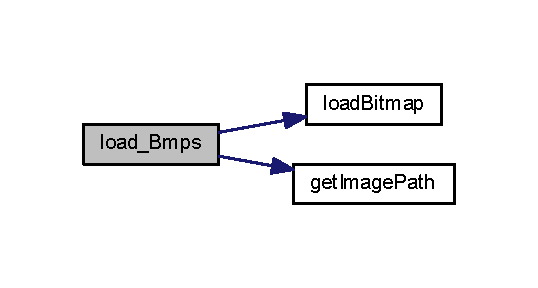
\includegraphics[width=258pt]{game_8h_a2d7ae67897b06ba4d723f059b8055c3d_cgraph}
\end{center}
\end{figure}
\hypertarget{game_8h_a7485cadb508c6cbe1efe9d01643b34e0}{}\label{game_8h_a7485cadb508c6cbe1efe9d01643b34e0} 
\index{game.\+h@{game.\+h}!mouse\+\_\+intrhandler@{mouse\+\_\+intrhandler}}
\index{mouse\+\_\+intrhandler@{mouse\+\_\+intrhandler}!game.\+h@{game.\+h}}
\subsubsection{\texorpdfstring{mouse\+\_\+intrhandler()}{mouse\_intrhandler()}}
{\footnotesize\ttfamily void mouse\+\_\+intrhandler (\begin{DoxyParamCaption}\item[{unsigned long}]{mouse\+\_\+packet\mbox{[}3\mbox{]},  }\item[{\hyperlink{structgame__t}{game\+\_\+t} $\ast$}]{game1 }\end{DoxyParamCaption})}



Handler for Mouse Interrupts. 


\begin{DoxyParams}{Parameters}
{\em mouse\+\_\+packet\mbox{[}3\mbox{]}} & Data packets of the Mouse \\
\hline
{\em $\ast$game1} & The game itself \\
\hline
\end{DoxyParams}
Here is the call graph for this function\+:
\nopagebreak
\begin{figure}[H]
\begin{center}
\leavevmode
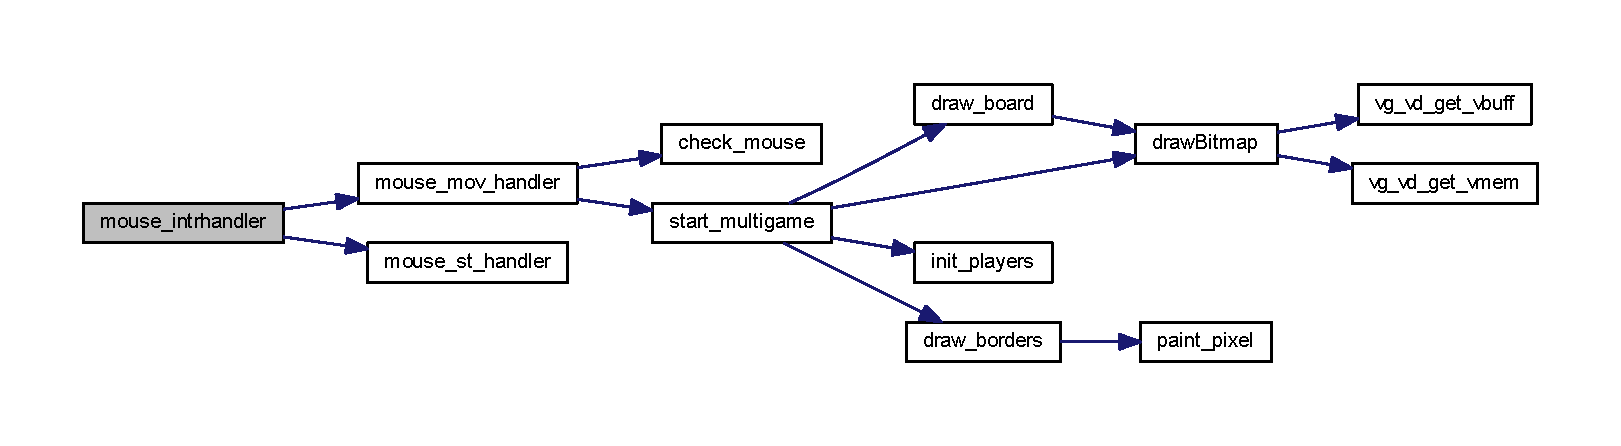
\includegraphics[width=350pt]{game_8h_a7485cadb508c6cbe1efe9d01643b34e0_cgraph}
\end{center}
\end{figure}
\hypertarget{game_8h_acde10310f33cafd602e547fdcc87e5f7}{}\label{game_8h_acde10310f33cafd602e547fdcc87e5f7} 
\index{game.\+h@{game.\+h}!mouse\+\_\+mov\+\_\+handler@{mouse\+\_\+mov\+\_\+handler}}
\index{mouse\+\_\+mov\+\_\+handler@{mouse\+\_\+mov\+\_\+handler}!game.\+h@{game.\+h}}
\subsubsection{\texorpdfstring{mouse\+\_\+mov\+\_\+handler()}{mouse\_mov\_handler()}}
{\footnotesize\ttfamily int mouse\+\_\+mov\+\_\+handler (\begin{DoxyParamCaption}\item[{unsigned long}]{mouse\+\_\+packet\mbox{[}3\mbox{]},  }\item[{\hyperlink{structgame__t}{game\+\_\+t} $\ast$}]{game1 }\end{DoxyParamCaption})}



Mouse Handler for Menu. 

Handles the buttons and movement of the mouse in the Menu


\begin{DoxyParams}{Parameters}
{\em mouse\+\_\+packet\mbox{[}3\mbox{]}} & Data packets of the Mouse \\
\hline
{\em $\ast$game1} & The game itself \\
\hline
\end{DoxyParams}
\begin{DoxyReturn}{Returns}
Return 1 on acceptable data and 0 if overflow 
\end{DoxyReturn}
Here is the call graph for this function\+:
\nopagebreak
\begin{figure}[H]
\begin{center}
\leavevmode
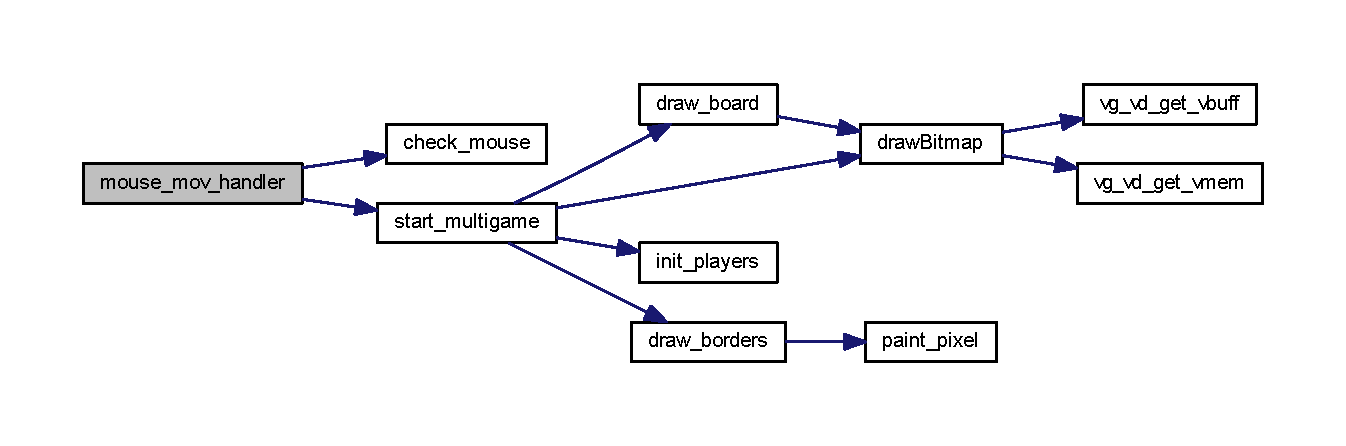
\includegraphics[width=350pt]{game_8h_acde10310f33cafd602e547fdcc87e5f7_cgraph}
\end{center}
\end{figure}
\hypertarget{game_8h_a5745594a9d371072ebddb008b3b08699}{}\label{game_8h_a5745594a9d371072ebddb008b3b08699} 
\index{game.\+h@{game.\+h}!mouse\+\_\+st\+\_\+handler@{mouse\+\_\+st\+\_\+handler}}
\index{mouse\+\_\+st\+\_\+handler@{mouse\+\_\+st\+\_\+handler}!game.\+h@{game.\+h}}
\subsubsection{\texorpdfstring{mouse\+\_\+st\+\_\+handler()}{mouse\_st\_handler()}}
{\footnotesize\ttfamily void mouse\+\_\+st\+\_\+handler (\begin{DoxyParamCaption}\item[{\hyperlink{structplayer__t}{player\+\_\+t} $\ast$}]{p,  }\item[{unsigned long}]{mouse\+\_\+packet\mbox{[}3\mbox{]},  }\item[{\hyperlink{structgame__t}{game\+\_\+t} $\ast$}]{game1 }\end{DoxyParamCaption})}



Mouse State Handler for Player 4. 


\begin{DoxyParams}{Parameters}
{\em $\ast$p} & Player \\
\hline
{\em mouse\+\_\+packet\mbox{[}3\mbox{]}} & Data packets of the Mouse \\
\hline
{\em $\ast$game1} & The game itself \\
\hline
\end{DoxyParams}
\hypertarget{game_8h_afdeb92b797c5bbc22fa9cea605f6644b}{}\label{game_8h_afdeb92b797c5bbc22fa9cea605f6644b} 
\index{game.\+h@{game.\+h}!playgame@{playgame}}
\index{playgame@{playgame}!game.\+h@{game.\+h}}
\subsubsection{\texorpdfstring{playgame()}{playgame()}}
{\footnotesize\ttfamily int playgame (\begin{DoxyParamCaption}\item[{\hyperlink{structgame__t}{game\+\_\+t} $\ast$}]{game1 }\end{DoxyParamCaption})}



The Game Function. 

Interrupts cycle


\begin{DoxyParams}{Parameters}
{\em $\ast$game1} & The game itself \\
\hline
\end{DoxyParams}
Here is the call graph for this function\+:
\nopagebreak
\begin{figure}[H]
\begin{center}
\leavevmode
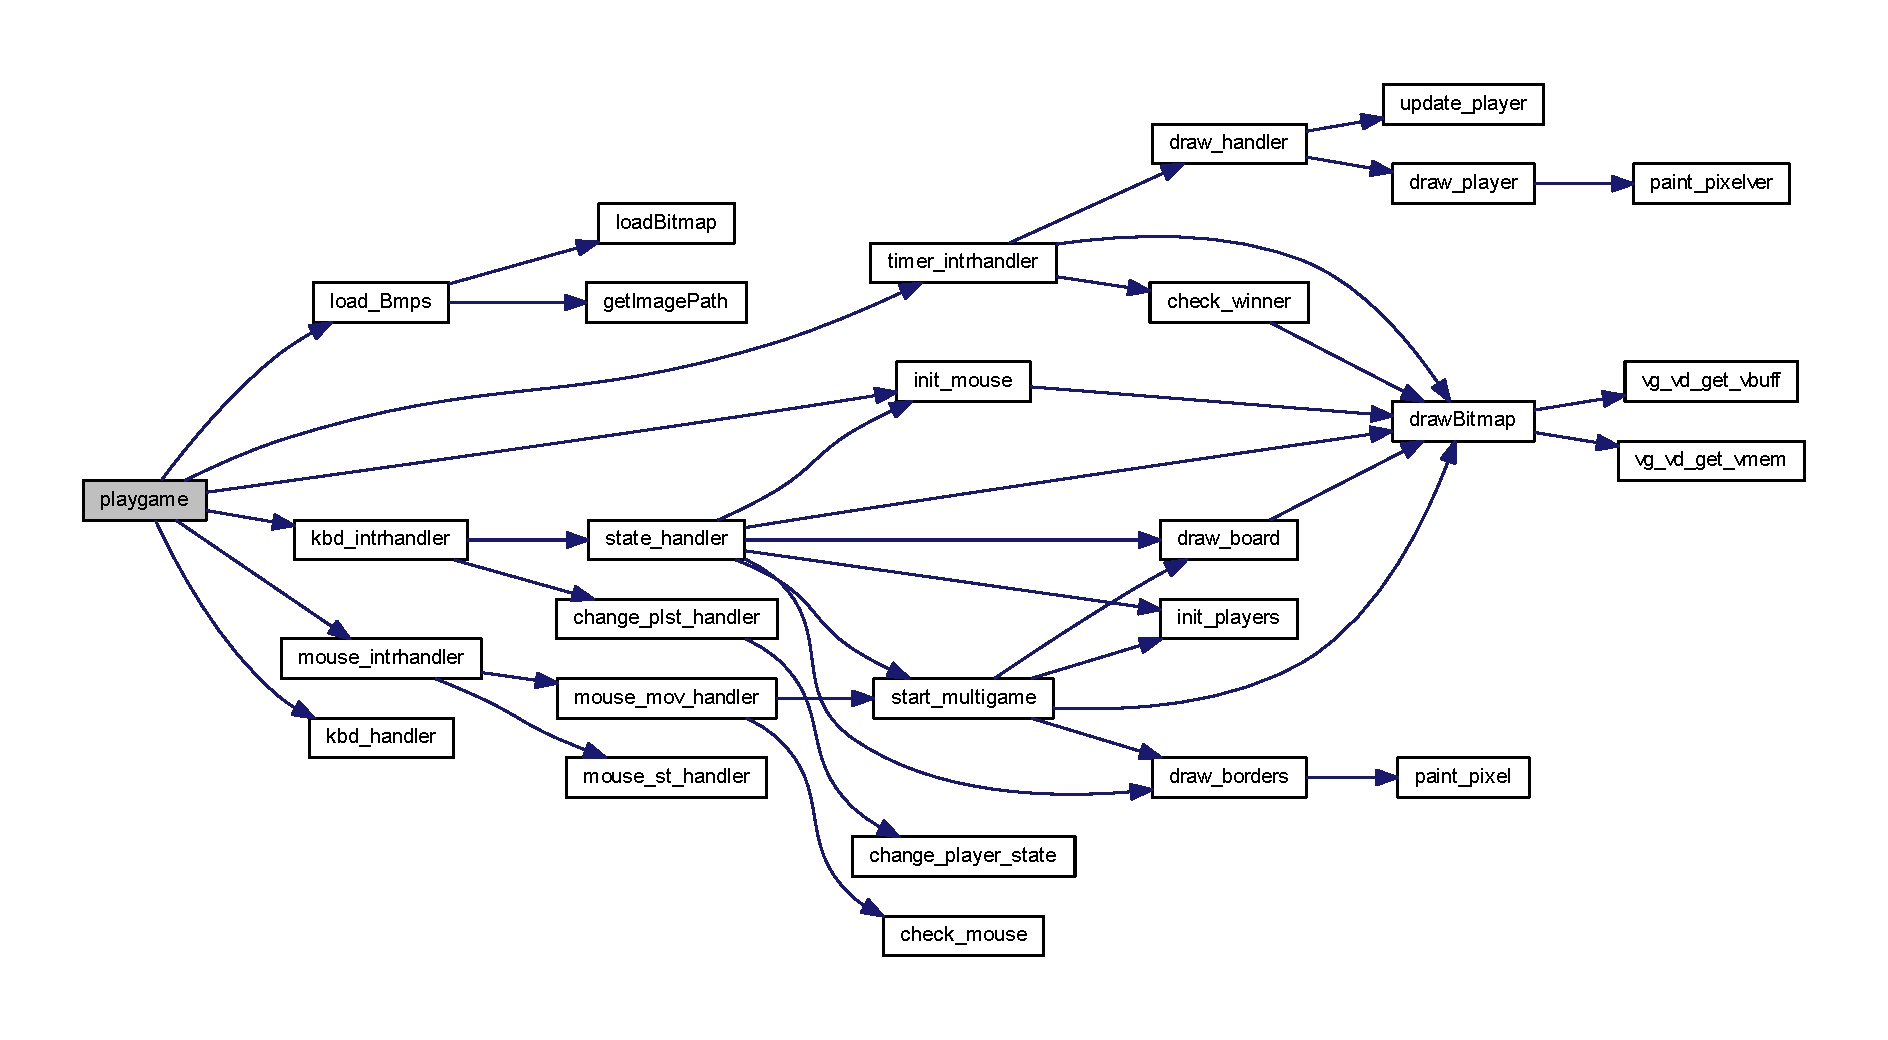
\includegraphics[width=350pt]{game_8h_afdeb92b797c5bbc22fa9cea605f6644b_cgraph}
\end{center}
\end{figure}
\hypertarget{game_8h_a59430d80f49694010887ac3ab116e696}{}\label{game_8h_a59430d80f49694010887ac3ab116e696} 
\index{game.\+h@{game.\+h}!start\+\_\+multigame@{start\+\_\+multigame}}
\index{start\+\_\+multigame@{start\+\_\+multigame}!game.\+h@{game.\+h}}
\subsubsection{\texorpdfstring{start\+\_\+multigame()}{start\_multigame()}}
{\footnotesize\ttfamily int start\+\_\+multigame (\begin{DoxyParamCaption}\item[{unsigned int}]{num\+\_\+players,  }\item[{\hyperlink{structgame__t}{game\+\_\+t} $\ast$}]{game1 }\end{DoxyParamCaption})}



Starts a Multiplayer Game accorgingly to the Number of Players. 


\begin{DoxyParams}{Parameters}
{\em num\+\_\+players} & Number of Players on the Game Mode \\
\hline
{\em $\ast$game1} & The game itself \\
\hline
\end{DoxyParams}
\begin{DoxyReturn}{Returns}
Return 0 on success and 1 otherwise 
\end{DoxyReturn}
Here is the call graph for this function\+:
\nopagebreak
\begin{figure}[H]
\begin{center}
\leavevmode
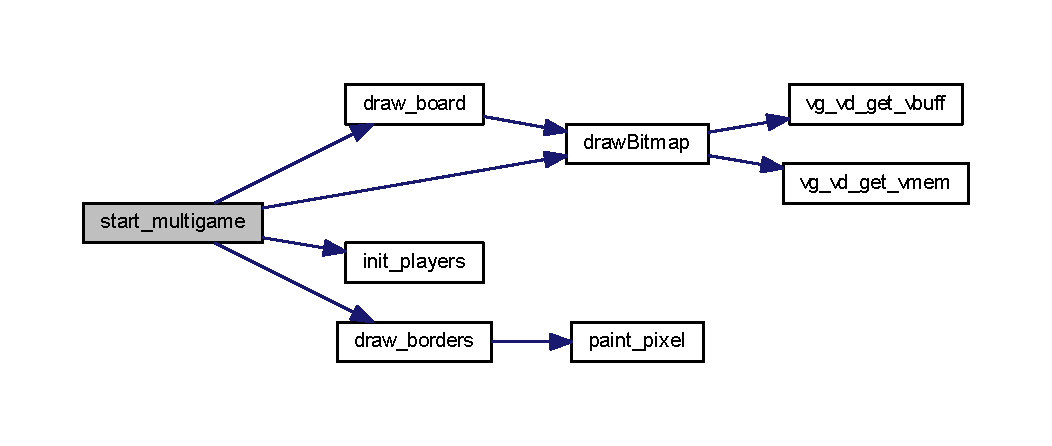
\includegraphics[width=350pt]{game_8h_a59430d80f49694010887ac3ab116e696_cgraph}
\end{center}
\end{figure}
\hypertarget{game_8h_a505eb2e66f358efafd4f23bca70cfa14}{}\label{game_8h_a505eb2e66f358efafd4f23bca70cfa14} 
\index{game.\+h@{game.\+h}!state\+\_\+handler@{state\+\_\+handler}}
\index{state\+\_\+handler@{state\+\_\+handler}!game.\+h@{game.\+h}}
\subsubsection{\texorpdfstring{state\+\_\+handler()}{state\_handler()}}
{\footnotesize\ttfamily void state\+\_\+handler (\begin{DoxyParamCaption}\item[{unsigned int}]{num\+\_\+players,  }\item[{unsigned long}]{data,  }\item[{\hyperlink{structgame__t}{game\+\_\+t} $\ast$}]{game1 }\end{DoxyParamCaption})}



Handler for Game States. 


\begin{DoxyParams}{Parameters}
{\em num\+\_\+players} & Number of Players in the current Game Mode \\
\hline
{\em data} & Keyboard data \\
\hline
{\em $\ast$game1} & The game itself \\
\hline
\end{DoxyParams}
Here is the call graph for this function\+:
\nopagebreak
\begin{figure}[H]
\begin{center}
\leavevmode
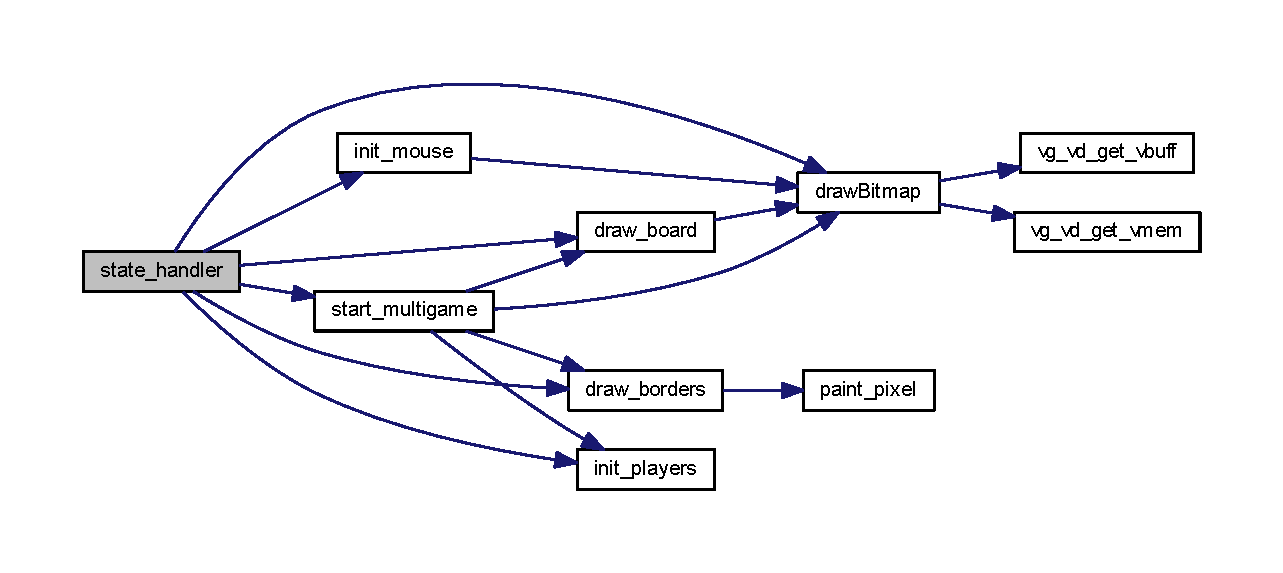
\includegraphics[width=350pt]{game_8h_a505eb2e66f358efafd4f23bca70cfa14_cgraph}
\end{center}
\end{figure}
\hypertarget{game_8h_a86358e01f0d51114bc31ea1b623ee024}{}\label{game_8h_a86358e01f0d51114bc31ea1b623ee024} 
\index{game.\+h@{game.\+h}!timer\+\_\+intrhandler@{timer\+\_\+intrhandler}}
\index{timer\+\_\+intrhandler@{timer\+\_\+intrhandler}!game.\+h@{game.\+h}}
\subsubsection{\texorpdfstring{timer\+\_\+intrhandler()}{timer\_intrhandler()}}
{\footnotesize\ttfamily void timer\+\_\+intrhandler (\begin{DoxyParamCaption}\item[{\hyperlink{structgame__t}{game\+\_\+t} $\ast$}]{game1 }\end{DoxyParamCaption})}



Handler for Timer Interrupts. 


\begin{DoxyParams}{Parameters}
{\em $\ast$game1} & The game itself \\
\hline
\end{DoxyParams}
Here is the call graph for this function\+:
\nopagebreak
\begin{figure}[H]
\begin{center}
\leavevmode
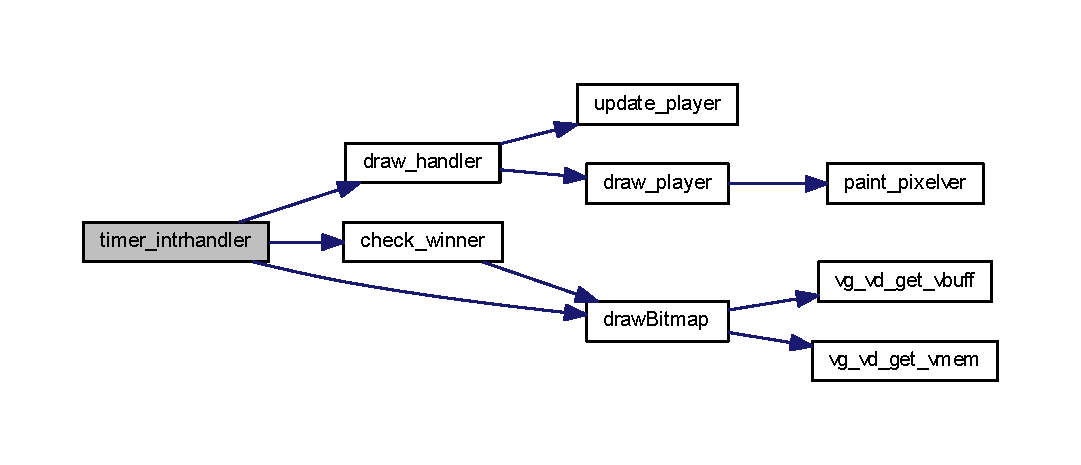
\includegraphics[width=350pt]{game_8h_a86358e01f0d51114bc31ea1b623ee024_cgraph}
\end{center}
\end{figure}
\hypertarget{game_8h_ab3383bfc12cb6695ede9ecd5f6573676}{}\label{game_8h_ab3383bfc12cb6695ede9ecd5f6573676} 
\index{game.\+h@{game.\+h}!update\+\_\+player@{update\+\_\+player}}
\index{update\+\_\+player@{update\+\_\+player}!game.\+h@{game.\+h}}
\subsubsection{\texorpdfstring{update\+\_\+player()}{update\_player()}}
{\footnotesize\ttfamily void update\+\_\+player (\begin{DoxyParamCaption}\item[{unsigned int}]{num\+\_\+players,  }\item[{\hyperlink{structgame__t}{game\+\_\+t} $\ast$}]{game1 }\end{DoxyParamCaption})}



Updates the position of a Player based on its movement. 


\begin{DoxyParams}{Parameters}
{\em num\+\_\+players} & Number of Players in the current Game Mode \\
\hline
{\em $\ast$game1} & The game itself \\
\hline
\end{DoxyParams}

\hypertarget{lmlib_8h}{}\section{C\+:/\+Users/jnuno/\+Desktop/src/lmlib.h File Reference}
\label{lmlib_8h}\index{C\+:/\+Users/jnuno/\+Desktop/src/lmlib.\+h@{C\+:/\+Users/jnuno/\+Desktop/src/lmlib.\+h}}
{\ttfamily \#include $<$minix/type.\+h$>$}\newline
Include dependency graph for lmlib.\+h\+:
\nopagebreak
\begin{figure}[H]
\begin{center}
\leavevmode
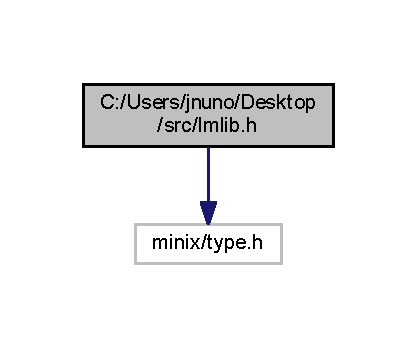
\includegraphics[width=200pt]{lmlib_8h__incl}
\end{center}
\end{figure}
This graph shows which files directly or indirectly include this file\+:
\nopagebreak
\begin{figure}[H]
\begin{center}
\leavevmode
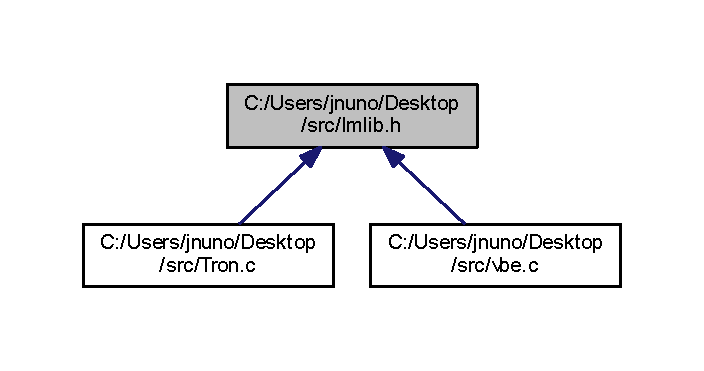
\includegraphics[width=338pt]{lmlib_8h__dep__incl}
\end{center}
\end{figure}
\subsection*{Data Structures}
\begin{DoxyCompactItemize}
\item 
struct \hyperlink{structmmap__t}{mmap\+\_\+t}
\end{DoxyCompactItemize}
\subsection*{Functions}
\begin{DoxyCompactItemize}
\item 
void $\ast$ \hyperlink{group__lmlib_ga00a9c17c01e794a6bfc80fc5c6ab1ed1}{lm\+\_\+init} (void)
\begin{DoxyCompactList}\small\item\em Initializes the low memory area, the region up to the 1 M\+Byte physical address, by mapping it on the process\textquotesingle{} physical memory address. \end{DoxyCompactList}\item 
void $\ast$ \hyperlink{group__lmlib_gae45d971ce2ffcf4dc2677eba033a92cd}{lm\+\_\+alloc} (unsigned long size, \hyperlink{structmmap__t}{mmap\+\_\+t} $\ast$map)
\begin{DoxyCompactList}\small\item\em Allocates a memory block in low memory area with the specified size. \end{DoxyCompactList}\item 
void \hyperlink{group__lmlib_ga73e89d9c297b7390021fb545513579c6}{lm\+\_\+free} (\hyperlink{structmmap__t}{mmap\+\_\+t} $\ast$map)
\begin{DoxyCompactList}\small\item\em Frees a memory block in the low memory area, previously allocated using \hyperlink{group__lmlib_gae45d971ce2ffcf4dc2677eba033a92cd}{lm\+\_\+alloc()} \end{DoxyCompactList}\end{DoxyCompactItemize}

\hypertarget{otherlabs_8c}{}\section{C\+:/\+Users/jnuno/\+Desktop/src/otherlabs.c File Reference}
\label{otherlabs_8c}\index{C\+:/\+Users/jnuno/\+Desktop/src/otherlabs.\+c@{C\+:/\+Users/jnuno/\+Desktop/src/otherlabs.\+c}}
{\ttfamily \#include $<$minix/syslib.\+h$>$}\newline
{\ttfamily \#include $<$minix/drivers.\+h$>$}\newline
{\ttfamily \#include $<$minix/com.\+h$>$}\newline
{\ttfamily \#include $<$minix/sysutil.\+h$>$}\newline
{\ttfamily \#include \char`\"{}tools.\+h\char`\"{}}\newline
{\ttfamily \#include \char`\"{}otherlabs.\+h\char`\"{}}\newline
Include dependency graph for otherlabs.\+c\+:
\nopagebreak
\begin{figure}[H]
\begin{center}
\leavevmode
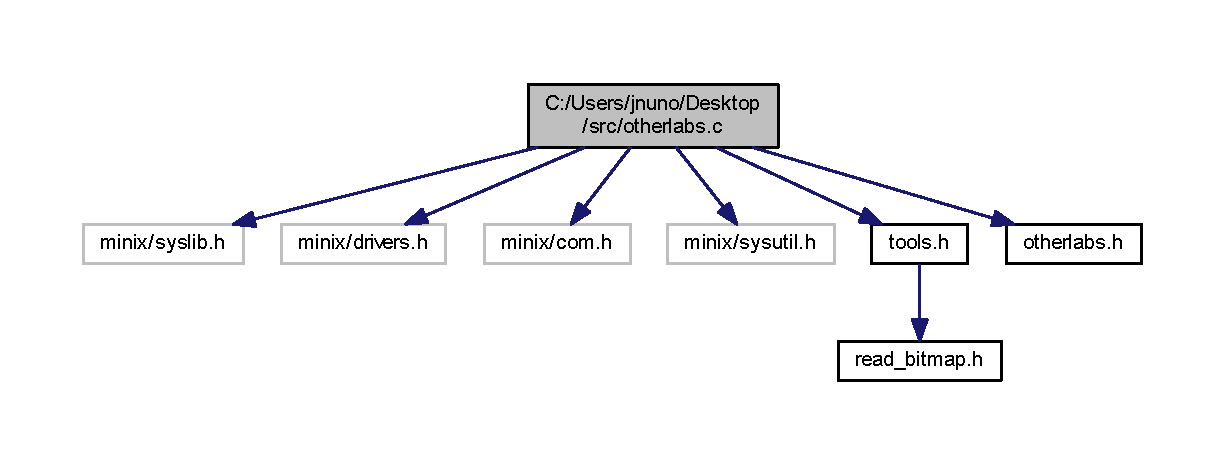
\includegraphics[width=350pt]{otherlabs_8c__incl}
\end{center}
\end{figure}
\subsection*{Functions}
\begin{DoxyCompactItemize}
\item 
int \hyperlink{otherlabs_8c_adb4846c9edc4417fbc70ec754f4c1682}{kbd\+\_\+subscribe\+\_\+int} (\hyperlink{structgame__t}{game\+\_\+t} $\ast$game1)
\begin{DoxyCompactList}\small\item\em Subscribes and enables Keyboard interrupts. \end{DoxyCompactList}\item 
int \hyperlink{otherlabs_8c_a2841bbbccfe026c4df7f6a98a5359d67}{kbd\+\_\+unsubscribe\+\_\+int} (\hyperlink{structgame__t}{game\+\_\+t} $\ast$game1)
\begin{DoxyCompactList}\small\item\em Unsubscribes Keyboard interrupts. \end{DoxyCompactList}\item 
int \hyperlink{otherlabs_8c_ab6fadc501bcb3a2a8d22f32c53a7e2bb}{timer\+\_\+subscribe\+\_\+int} (\hyperlink{structgame__t}{game\+\_\+t} $\ast$game1)
\begin{DoxyCompactList}\small\item\em Subscribes and enables Timer 0 interrupts. \end{DoxyCompactList}\item 
int \hyperlink{otherlabs_8c_ae0888c4f8f20af35339447b3f228b884}{timer\+\_\+unsubscribe\+\_\+int} (\hyperlink{structgame__t}{game\+\_\+t} $\ast$game1)
\begin{DoxyCompactList}\small\item\em Unsubscribes Timer 0 interrupts. \end{DoxyCompactList}\item 
int \hyperlink{otherlabs_8c_a37eae8196ee38ff2a9d9d431e91dac91}{mouse\+\_\+subscribe\+\_\+int} (\hyperlink{structgame__t}{game\+\_\+t} $\ast$game1)
\begin{DoxyCompactList}\small\item\em Subscribes and enables Mouse interrupts. \end{DoxyCompactList}\item 
int \hyperlink{otherlabs_8c_a04fb2b0c0c20492e9e94277c84b37cd9}{mouse\+\_\+unsubscribe\+\_\+int} (\hyperlink{structgame__t}{game\+\_\+t} $\ast$game1)
\begin{DoxyCompactList}\small\item\em Unsubscribes Mouse interrupts. \end{DoxyCompactList}\item 
int \hyperlink{otherlabs_8c_a13393ae743886637e81723f6177e0ad1}{sub\+\_\+game} (\hyperlink{structgame__t}{game\+\_\+t} $\ast$game1)
\begin{DoxyCompactList}\small\item\em Subscribe Handler. \end{DoxyCompactList}\item 
int \hyperlink{otherlabs_8c_aeda1f986abc84e2fffa1c47aff4c4ad7}{unsub\+\_\+game} (\hyperlink{structgame__t}{game\+\_\+t} $\ast$game1)
\begin{DoxyCompactList}\small\item\em Unsubscribe Handler. \end{DoxyCompactList}\item 
unsigned long \hyperlink{otherlabs_8c_a148728381af10708c1d48f6f892fd9dd}{kbd\+\_\+handler} ()
\begin{DoxyCompactList}\small\item\em Keyboard Interrupt Reader. \end{DoxyCompactList}\item 
int \hyperlink{otherlabs_8c_a00b569b833191afad3a893b774cfd546}{kbd\+\_\+send\+\_\+command} (unsigned long cmd)
\begin{DoxyCompactList}\small\item\em Send Command to Keyboard Command Register(port 0x64) \end{DoxyCompactList}\item 
int \hyperlink{otherlabs_8c_a816e7f217f9a42aa198789bae26fbf95}{kbd\+\_\+send} (unsigned long cmd)
\begin{DoxyCompactList}\small\item\em Send Command to Keyboard Data Buffer(port 0x60) \end{DoxyCompactList}\item 
int \hyperlink{otherlabs_8c_abb4d7e40999509e678e49d16c58b93c2}{mouse\+\_\+send} (unsigned long cmd)
\begin{DoxyCompactList}\small\item\em Handler to send commands to keyboard register. \end{DoxyCompactList}\end{DoxyCompactItemize}


\subsection{Function Documentation}
\hypertarget{otherlabs_8c_a148728381af10708c1d48f6f892fd9dd}{}\label{otherlabs_8c_a148728381af10708c1d48f6f892fd9dd} 
\index{otherlabs.\+c@{otherlabs.\+c}!kbd\+\_\+handler@{kbd\+\_\+handler}}
\index{kbd\+\_\+handler@{kbd\+\_\+handler}!otherlabs.\+c@{otherlabs.\+c}}
\subsubsection{\texorpdfstring{kbd\+\_\+handler()}{kbd\_handler()}}
{\footnotesize\ttfamily unsigned long kbd\+\_\+handler (\begin{DoxyParamCaption}{ }\end{DoxyParamCaption})}



Keyboard Interrupt Reader. 

Reads from the Keyboard Output Buffer

\begin{DoxyReturn}{Returns}
Return -\/1 upon failure and the data read otherwise 
\end{DoxyReturn}
\hypertarget{otherlabs_8c_a816e7f217f9a42aa198789bae26fbf95}{}\label{otherlabs_8c_a816e7f217f9a42aa198789bae26fbf95} 
\index{otherlabs.\+c@{otherlabs.\+c}!kbd\+\_\+send@{kbd\+\_\+send}}
\index{kbd\+\_\+send@{kbd\+\_\+send}!otherlabs.\+c@{otherlabs.\+c}}
\subsubsection{\texorpdfstring{kbd\+\_\+send()}{kbd\_send()}}
{\footnotesize\ttfamily int kbd\+\_\+send (\begin{DoxyParamCaption}\item[{unsigned long}]{cmd }\end{DoxyParamCaption})}



Send Command to Keyboard Data Buffer(port 0x60) 


\begin{DoxyParams}{Parameters}
{\em cmd} & Command to send \\
\hline
\end{DoxyParams}
\begin{DoxyReturn}{Returns}
Return -\/1 upon failure and 0 otherwise 
\end{DoxyReturn}
\hypertarget{otherlabs_8c_a00b569b833191afad3a893b774cfd546}{}\label{otherlabs_8c_a00b569b833191afad3a893b774cfd546} 
\index{otherlabs.\+c@{otherlabs.\+c}!kbd\+\_\+send\+\_\+command@{kbd\+\_\+send\+\_\+command}}
\index{kbd\+\_\+send\+\_\+command@{kbd\+\_\+send\+\_\+command}!otherlabs.\+c@{otherlabs.\+c}}
\subsubsection{\texorpdfstring{kbd\+\_\+send\+\_\+command()}{kbd\_send\_command()}}
{\footnotesize\ttfamily int kbd\+\_\+send\+\_\+command (\begin{DoxyParamCaption}\item[{unsigned long}]{cmd }\end{DoxyParamCaption})}



Send Command to Keyboard Command Register(port 0x64) 


\begin{DoxyParams}{Parameters}
{\em cmd} & Command to send \\
\hline
\end{DoxyParams}
\begin{DoxyReturn}{Returns}
Return -\/1 upon failure and 0 otherwise 
\end{DoxyReturn}
\hypertarget{otherlabs_8c_adb4846c9edc4417fbc70ec754f4c1682}{}\label{otherlabs_8c_adb4846c9edc4417fbc70ec754f4c1682} 
\index{otherlabs.\+c@{otherlabs.\+c}!kbd\+\_\+subscribe\+\_\+int@{kbd\+\_\+subscribe\+\_\+int}}
\index{kbd\+\_\+subscribe\+\_\+int@{kbd\+\_\+subscribe\+\_\+int}!otherlabs.\+c@{otherlabs.\+c}}
\subsubsection{\texorpdfstring{kbd\+\_\+subscribe\+\_\+int()}{kbd\_subscribe\_int()}}
{\footnotesize\ttfamily int kbd\+\_\+subscribe\+\_\+int (\begin{DoxyParamCaption}\item[{\hyperlink{structgame__t}{game\+\_\+t} $\ast$}]{game1 }\end{DoxyParamCaption})}



Subscribes and enables Keyboard interrupts. 

\begin{DoxyReturn}{Returns}
Returns bit order in interrupt mask; negative value on failure 
\end{DoxyReturn}
\hypertarget{otherlabs_8c_a2841bbbccfe026c4df7f6a98a5359d67}{}\label{otherlabs_8c_a2841bbbccfe026c4df7f6a98a5359d67} 
\index{otherlabs.\+c@{otherlabs.\+c}!kbd\+\_\+unsubscribe\+\_\+int@{kbd\+\_\+unsubscribe\+\_\+int}}
\index{kbd\+\_\+unsubscribe\+\_\+int@{kbd\+\_\+unsubscribe\+\_\+int}!otherlabs.\+c@{otherlabs.\+c}}
\subsubsection{\texorpdfstring{kbd\+\_\+unsubscribe\+\_\+int()}{kbd\_unsubscribe\_int()}}
{\footnotesize\ttfamily int kbd\+\_\+unsubscribe\+\_\+int (\begin{DoxyParamCaption}\item[{\hyperlink{structgame__t}{game\+\_\+t} $\ast$}]{game1 }\end{DoxyParamCaption})}



Unsubscribes Keyboard interrupts. 

\begin{DoxyReturn}{Returns}
Return 0 upon success and non-\/zero otherwise 
\end{DoxyReturn}
\hypertarget{otherlabs_8c_abb4d7e40999509e678e49d16c58b93c2}{}\label{otherlabs_8c_abb4d7e40999509e678e49d16c58b93c2} 
\index{otherlabs.\+c@{otherlabs.\+c}!mouse\+\_\+send@{mouse\+\_\+send}}
\index{mouse\+\_\+send@{mouse\+\_\+send}!otherlabs.\+c@{otherlabs.\+c}}
\subsubsection{\texorpdfstring{mouse\+\_\+send()}{mouse\_send()}}
{\footnotesize\ttfamily int mouse\+\_\+send (\begin{DoxyParamCaption}\item[{unsigned long}]{cmd }\end{DoxyParamCaption})}



Handler to send commands to keyboard register. 


\begin{DoxyParams}{Parameters}
{\em cmd} & Command to send \\
\hline
\end{DoxyParams}
\begin{DoxyReturn}{Returns}
Return 1 upon failure and 0 otherwise 
\end{DoxyReturn}
Here is the call graph for this function\+:
\nopagebreak
\begin{figure}[H]
\begin{center}
\leavevmode
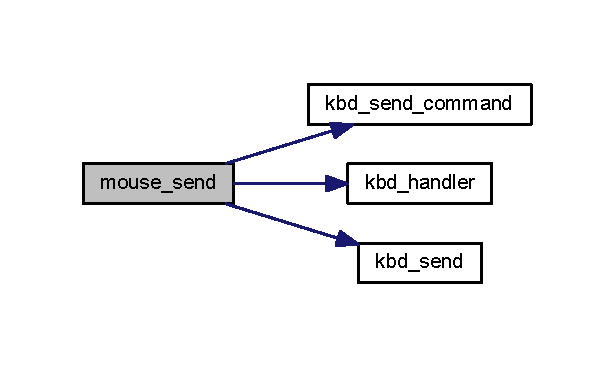
\includegraphics[width=295pt]{otherlabs_8c_abb4d7e40999509e678e49d16c58b93c2_cgraph}
\end{center}
\end{figure}
\hypertarget{otherlabs_8c_a37eae8196ee38ff2a9d9d431e91dac91}{}\label{otherlabs_8c_a37eae8196ee38ff2a9d9d431e91dac91} 
\index{otherlabs.\+c@{otherlabs.\+c}!mouse\+\_\+subscribe\+\_\+int@{mouse\+\_\+subscribe\+\_\+int}}
\index{mouse\+\_\+subscribe\+\_\+int@{mouse\+\_\+subscribe\+\_\+int}!otherlabs.\+c@{otherlabs.\+c}}
\subsubsection{\texorpdfstring{mouse\+\_\+subscribe\+\_\+int()}{mouse\_subscribe\_int()}}
{\footnotesize\ttfamily int mouse\+\_\+subscribe\+\_\+int (\begin{DoxyParamCaption}\item[{\hyperlink{structgame__t}{game\+\_\+t} $\ast$}]{game1 }\end{DoxyParamCaption})}



Subscribes and enables Mouse interrupts. 

\begin{DoxyReturn}{Returns}
Returns bit order in interrupt mask; negative value on failure 
\end{DoxyReturn}
\hypertarget{otherlabs_8c_a04fb2b0c0c20492e9e94277c84b37cd9}{}\label{otherlabs_8c_a04fb2b0c0c20492e9e94277c84b37cd9} 
\index{otherlabs.\+c@{otherlabs.\+c}!mouse\+\_\+unsubscribe\+\_\+int@{mouse\+\_\+unsubscribe\+\_\+int}}
\index{mouse\+\_\+unsubscribe\+\_\+int@{mouse\+\_\+unsubscribe\+\_\+int}!otherlabs.\+c@{otherlabs.\+c}}
\subsubsection{\texorpdfstring{mouse\+\_\+unsubscribe\+\_\+int()}{mouse\_unsubscribe\_int()}}
{\footnotesize\ttfamily int mouse\+\_\+unsubscribe\+\_\+int (\begin{DoxyParamCaption}\item[{\hyperlink{structgame__t}{game\+\_\+t} $\ast$}]{game1 }\end{DoxyParamCaption})}



Unsubscribes Mouse interrupts. 

\begin{DoxyReturn}{Returns}
Return 0 upon success and non-\/zero otherwise 
\end{DoxyReturn}
\hypertarget{otherlabs_8c_a13393ae743886637e81723f6177e0ad1}{}\label{otherlabs_8c_a13393ae743886637e81723f6177e0ad1} 
\index{otherlabs.\+c@{otherlabs.\+c}!sub\+\_\+game@{sub\+\_\+game}}
\index{sub\+\_\+game@{sub\+\_\+game}!otherlabs.\+c@{otherlabs.\+c}}
\subsubsection{\texorpdfstring{sub\+\_\+game()}{sub\_game()}}
{\footnotesize\ttfamily int sub\+\_\+game (\begin{DoxyParamCaption}\item[{\hyperlink{structgame__t}{game\+\_\+t} $\ast$}]{game1 }\end{DoxyParamCaption})}



Subscribe Handler. 

Calls the Timer 0, Keyboard and Mouse interrupts subscription functions

\begin{DoxyReturn}{Returns}
Return 0 upon success and non-\/zero otherwise 
\end{DoxyReturn}
Here is the call graph for this function\+:
\nopagebreak
\begin{figure}[H]
\begin{center}
\leavevmode
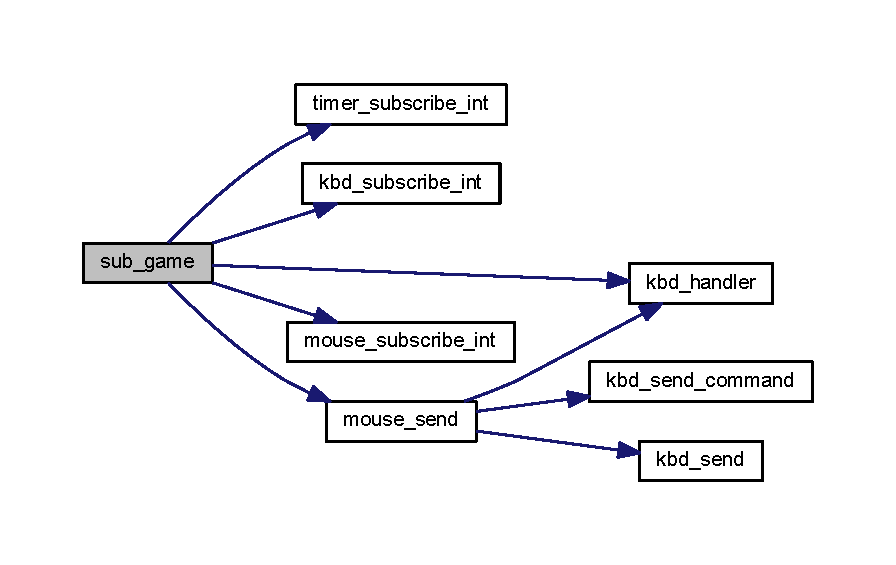
\includegraphics[width=350pt]{otherlabs_8c_a13393ae743886637e81723f6177e0ad1_cgraph}
\end{center}
\end{figure}
\hypertarget{otherlabs_8c_ab6fadc501bcb3a2a8d22f32c53a7e2bb}{}\label{otherlabs_8c_ab6fadc501bcb3a2a8d22f32c53a7e2bb} 
\index{otherlabs.\+c@{otherlabs.\+c}!timer\+\_\+subscribe\+\_\+int@{timer\+\_\+subscribe\+\_\+int}}
\index{timer\+\_\+subscribe\+\_\+int@{timer\+\_\+subscribe\+\_\+int}!otherlabs.\+c@{otherlabs.\+c}}
\subsubsection{\texorpdfstring{timer\+\_\+subscribe\+\_\+int()}{timer\_subscribe\_int()}}
{\footnotesize\ttfamily int timer\+\_\+subscribe\+\_\+int (\begin{DoxyParamCaption}\item[{\hyperlink{structgame__t}{game\+\_\+t} $\ast$}]{game1 }\end{DoxyParamCaption})}



Subscribes and enables Timer 0 interrupts. 

\begin{DoxyReturn}{Returns}
Returns bit order in interrupt mask; negative value on failure 
\end{DoxyReturn}
\hypertarget{otherlabs_8c_ae0888c4f8f20af35339447b3f228b884}{}\label{otherlabs_8c_ae0888c4f8f20af35339447b3f228b884} 
\index{otherlabs.\+c@{otherlabs.\+c}!timer\+\_\+unsubscribe\+\_\+int@{timer\+\_\+unsubscribe\+\_\+int}}
\index{timer\+\_\+unsubscribe\+\_\+int@{timer\+\_\+unsubscribe\+\_\+int}!otherlabs.\+c@{otherlabs.\+c}}
\subsubsection{\texorpdfstring{timer\+\_\+unsubscribe\+\_\+int()}{timer\_unsubscribe\_int()}}
{\footnotesize\ttfamily int timer\+\_\+unsubscribe\+\_\+int (\begin{DoxyParamCaption}\item[{\hyperlink{structgame__t}{game\+\_\+t} $\ast$}]{game1 }\end{DoxyParamCaption})}



Unsubscribes Timer 0 interrupts. 

\begin{DoxyReturn}{Returns}
Return 0 upon success and non-\/zero otherwise 
\end{DoxyReturn}
\hypertarget{otherlabs_8c_aeda1f986abc84e2fffa1c47aff4c4ad7}{}\label{otherlabs_8c_aeda1f986abc84e2fffa1c47aff4c4ad7} 
\index{otherlabs.\+c@{otherlabs.\+c}!unsub\+\_\+game@{unsub\+\_\+game}}
\index{unsub\+\_\+game@{unsub\+\_\+game}!otherlabs.\+c@{otherlabs.\+c}}
\subsubsection{\texorpdfstring{unsub\+\_\+game()}{unsub\_game()}}
{\footnotesize\ttfamily int unsub\+\_\+game (\begin{DoxyParamCaption}\item[{\hyperlink{structgame__t}{game\+\_\+t} $\ast$}]{game1 }\end{DoxyParamCaption})}



Unsubscribe Handler. 

Calls the Timer 0, Keyboard and Mouse interrupts unsubscription functions

\begin{DoxyReturn}{Returns}
Return 0 upon success and non-\/zero otherwise 
\end{DoxyReturn}
Here is the call graph for this function\+:
\nopagebreak
\begin{figure}[H]
\begin{center}
\leavevmode
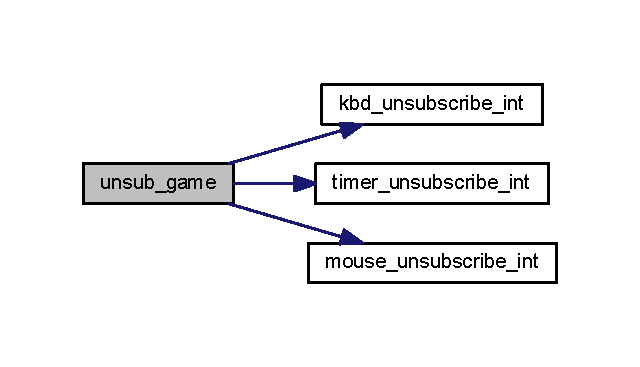
\includegraphics[width=307pt]{otherlabs_8c_aeda1f986abc84e2fffa1c47aff4c4ad7_cgraph}
\end{center}
\end{figure}

\hypertarget{otherlabs_8h}{}\section{C\+:/\+Users/jnuno/\+Desktop/src/otherlabs.h File Reference}
\label{otherlabs_8h}\index{C\+:/\+Users/jnuno/\+Desktop/src/otherlabs.\+h@{C\+:/\+Users/jnuno/\+Desktop/src/otherlabs.\+h}}
This graph shows which files directly or indirectly include this file\+:
\nopagebreak
\begin{figure}[H]
\begin{center}
\leavevmode
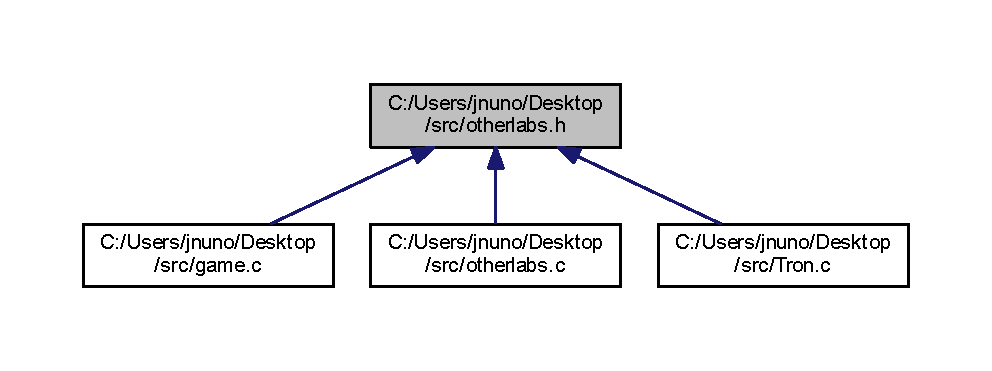
\includegraphics[width=350pt]{otherlabs_8h__dep__incl}
\end{center}
\end{figure}
\subsection*{Functions}
\begin{DoxyCompactItemize}
\item 
int \hyperlink{otherlabs_8h_adb4846c9edc4417fbc70ec754f4c1682}{kbd\+\_\+subscribe\+\_\+int} (\hyperlink{structgame__t}{game\+\_\+t} $\ast$game1)
\begin{DoxyCompactList}\small\item\em Subscribes and enables Keyboard interrupts. \end{DoxyCompactList}\item 
int \hyperlink{otherlabs_8h_a2841bbbccfe026c4df7f6a98a5359d67}{kbd\+\_\+unsubscribe\+\_\+int} (\hyperlink{structgame__t}{game\+\_\+t} $\ast$game1)
\begin{DoxyCompactList}\small\item\em Unsubscribes Keyboard interrupts. \end{DoxyCompactList}\item 
int \hyperlink{otherlabs_8h_ab6fadc501bcb3a2a8d22f32c53a7e2bb}{timer\+\_\+subscribe\+\_\+int} (\hyperlink{structgame__t}{game\+\_\+t} $\ast$game1)
\begin{DoxyCompactList}\small\item\em Subscribes and enables Timer 0 interrupts. \end{DoxyCompactList}\item 
int \hyperlink{otherlabs_8h_ae0888c4f8f20af35339447b3f228b884}{timer\+\_\+unsubscribe\+\_\+int} (\hyperlink{structgame__t}{game\+\_\+t} $\ast$game1)
\begin{DoxyCompactList}\small\item\em Unsubscribes Timer 0 interrupts. \end{DoxyCompactList}\item 
int \hyperlink{otherlabs_8h_a37eae8196ee38ff2a9d9d431e91dac91}{mouse\+\_\+subscribe\+\_\+int} (\hyperlink{structgame__t}{game\+\_\+t} $\ast$game1)
\begin{DoxyCompactList}\small\item\em Subscribes and enables Mouse interrupts. \end{DoxyCompactList}\item 
int \hyperlink{otherlabs_8h_a04fb2b0c0c20492e9e94277c84b37cd9}{mouse\+\_\+unsubscribe\+\_\+int} (\hyperlink{structgame__t}{game\+\_\+t} $\ast$game1)
\begin{DoxyCompactList}\small\item\em Unsubscribes Mouse interrupts. \end{DoxyCompactList}\item 
int \hyperlink{otherlabs_8h_a13393ae743886637e81723f6177e0ad1}{sub\+\_\+game} (\hyperlink{structgame__t}{game\+\_\+t} $\ast$game1)
\begin{DoxyCompactList}\small\item\em Subscribe Handler. \end{DoxyCompactList}\item 
int \hyperlink{otherlabs_8h_aeda1f986abc84e2fffa1c47aff4c4ad7}{unsub\+\_\+game} (\hyperlink{structgame__t}{game\+\_\+t} $\ast$game1)
\begin{DoxyCompactList}\small\item\em Unsubscribe Handler. \end{DoxyCompactList}\item 
unsigned long \hyperlink{otherlabs_8h_a148728381af10708c1d48f6f892fd9dd}{kbd\+\_\+handler} ()
\begin{DoxyCompactList}\small\item\em Keyboard Interrupt Reader. \end{DoxyCompactList}\item 
int \hyperlink{otherlabs_8h_a00b569b833191afad3a893b774cfd546}{kbd\+\_\+send\+\_\+command} (unsigned long cmd)
\begin{DoxyCompactList}\small\item\em Send Command to Keyboard Command Register(port 0x64) \end{DoxyCompactList}\item 
int \hyperlink{otherlabs_8h_a816e7f217f9a42aa198789bae26fbf95}{kbd\+\_\+send} (unsigned long cmd)
\begin{DoxyCompactList}\small\item\em Send Command to Keyboard Data Buffer(port 0x60) \end{DoxyCompactList}\item 
int \hyperlink{otherlabs_8h_abb4d7e40999509e678e49d16c58b93c2}{mouse\+\_\+send} (unsigned long cmd)
\begin{DoxyCompactList}\small\item\em Handler to send commands to keyboard register. \end{DoxyCompactList}\end{DoxyCompactItemize}


\subsection{Function Documentation}
\hypertarget{otherlabs_8h_a148728381af10708c1d48f6f892fd9dd}{}\label{otherlabs_8h_a148728381af10708c1d48f6f892fd9dd} 
\index{otherlabs.\+h@{otherlabs.\+h}!kbd\+\_\+handler@{kbd\+\_\+handler}}
\index{kbd\+\_\+handler@{kbd\+\_\+handler}!otherlabs.\+h@{otherlabs.\+h}}
\subsubsection{\texorpdfstring{kbd\+\_\+handler()}{kbd\_handler()}}
{\footnotesize\ttfamily unsigned long kbd\+\_\+handler (\begin{DoxyParamCaption}{ }\end{DoxyParamCaption})}



Keyboard Interrupt Reader. 

Reads from the Keyboard Output Buffer

\begin{DoxyReturn}{Returns}
Return -\/1 upon failure and the data read otherwise 
\end{DoxyReturn}
\hypertarget{otherlabs_8h_a816e7f217f9a42aa198789bae26fbf95}{}\label{otherlabs_8h_a816e7f217f9a42aa198789bae26fbf95} 
\index{otherlabs.\+h@{otherlabs.\+h}!kbd\+\_\+send@{kbd\+\_\+send}}
\index{kbd\+\_\+send@{kbd\+\_\+send}!otherlabs.\+h@{otherlabs.\+h}}
\subsubsection{\texorpdfstring{kbd\+\_\+send()}{kbd\_send()}}
{\footnotesize\ttfamily int kbd\+\_\+send (\begin{DoxyParamCaption}\item[{unsigned long}]{cmd }\end{DoxyParamCaption})}



Send Command to Keyboard Data Buffer(port 0x60) 


\begin{DoxyParams}{Parameters}
{\em cmd} & Command to send \\
\hline
\end{DoxyParams}
\begin{DoxyReturn}{Returns}
Return -\/1 upon failure and 0 otherwise 
\end{DoxyReturn}
\hypertarget{otherlabs_8h_a00b569b833191afad3a893b774cfd546}{}\label{otherlabs_8h_a00b569b833191afad3a893b774cfd546} 
\index{otherlabs.\+h@{otherlabs.\+h}!kbd\+\_\+send\+\_\+command@{kbd\+\_\+send\+\_\+command}}
\index{kbd\+\_\+send\+\_\+command@{kbd\+\_\+send\+\_\+command}!otherlabs.\+h@{otherlabs.\+h}}
\subsubsection{\texorpdfstring{kbd\+\_\+send\+\_\+command()}{kbd\_send\_command()}}
{\footnotesize\ttfamily int kbd\+\_\+send\+\_\+command (\begin{DoxyParamCaption}\item[{unsigned long}]{cmd }\end{DoxyParamCaption})}



Send Command to Keyboard Command Register(port 0x64) 


\begin{DoxyParams}{Parameters}
{\em cmd} & Command to send \\
\hline
\end{DoxyParams}
\begin{DoxyReturn}{Returns}
Return -\/1 upon failure and 0 otherwise 
\end{DoxyReturn}
\hypertarget{otherlabs_8h_adb4846c9edc4417fbc70ec754f4c1682}{}\label{otherlabs_8h_adb4846c9edc4417fbc70ec754f4c1682} 
\index{otherlabs.\+h@{otherlabs.\+h}!kbd\+\_\+subscribe\+\_\+int@{kbd\+\_\+subscribe\+\_\+int}}
\index{kbd\+\_\+subscribe\+\_\+int@{kbd\+\_\+subscribe\+\_\+int}!otherlabs.\+h@{otherlabs.\+h}}
\subsubsection{\texorpdfstring{kbd\+\_\+subscribe\+\_\+int()}{kbd\_subscribe\_int()}}
{\footnotesize\ttfamily int kbd\+\_\+subscribe\+\_\+int (\begin{DoxyParamCaption}\item[{\hyperlink{structgame__t}{game\+\_\+t} $\ast$}]{game1 }\end{DoxyParamCaption})}



Subscribes and enables Keyboard interrupts. 

\begin{DoxyReturn}{Returns}
Returns bit order in interrupt mask; negative value on failure 
\end{DoxyReturn}
\hypertarget{otherlabs_8h_a2841bbbccfe026c4df7f6a98a5359d67}{}\label{otherlabs_8h_a2841bbbccfe026c4df7f6a98a5359d67} 
\index{otherlabs.\+h@{otherlabs.\+h}!kbd\+\_\+unsubscribe\+\_\+int@{kbd\+\_\+unsubscribe\+\_\+int}}
\index{kbd\+\_\+unsubscribe\+\_\+int@{kbd\+\_\+unsubscribe\+\_\+int}!otherlabs.\+h@{otherlabs.\+h}}
\subsubsection{\texorpdfstring{kbd\+\_\+unsubscribe\+\_\+int()}{kbd\_unsubscribe\_int()}}
{\footnotesize\ttfamily int kbd\+\_\+unsubscribe\+\_\+int (\begin{DoxyParamCaption}\item[{\hyperlink{structgame__t}{game\+\_\+t} $\ast$}]{game1 }\end{DoxyParamCaption})}



Unsubscribes Keyboard interrupts. 

\begin{DoxyReturn}{Returns}
Return 0 upon success and non-\/zero otherwise 
\end{DoxyReturn}
\hypertarget{otherlabs_8h_abb4d7e40999509e678e49d16c58b93c2}{}\label{otherlabs_8h_abb4d7e40999509e678e49d16c58b93c2} 
\index{otherlabs.\+h@{otherlabs.\+h}!mouse\+\_\+send@{mouse\+\_\+send}}
\index{mouse\+\_\+send@{mouse\+\_\+send}!otherlabs.\+h@{otherlabs.\+h}}
\subsubsection{\texorpdfstring{mouse\+\_\+send()}{mouse\_send()}}
{\footnotesize\ttfamily int mouse\+\_\+send (\begin{DoxyParamCaption}\item[{unsigned long}]{cmd }\end{DoxyParamCaption})}



Handler to send commands to keyboard register. 


\begin{DoxyParams}{Parameters}
{\em cmd} & Command to send \\
\hline
\end{DoxyParams}
\begin{DoxyReturn}{Returns}
Return 1 upon failure and 0 otherwise 
\end{DoxyReturn}
Here is the call graph for this function\+:
\nopagebreak
\begin{figure}[H]
\begin{center}
\leavevmode
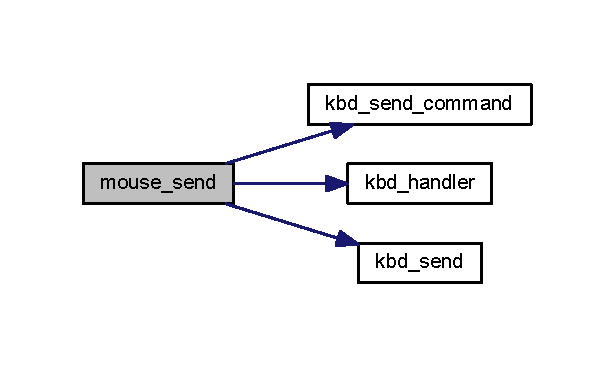
\includegraphics[width=295pt]{otherlabs_8h_abb4d7e40999509e678e49d16c58b93c2_cgraph}
\end{center}
\end{figure}
\hypertarget{otherlabs_8h_a37eae8196ee38ff2a9d9d431e91dac91}{}\label{otherlabs_8h_a37eae8196ee38ff2a9d9d431e91dac91} 
\index{otherlabs.\+h@{otherlabs.\+h}!mouse\+\_\+subscribe\+\_\+int@{mouse\+\_\+subscribe\+\_\+int}}
\index{mouse\+\_\+subscribe\+\_\+int@{mouse\+\_\+subscribe\+\_\+int}!otherlabs.\+h@{otherlabs.\+h}}
\subsubsection{\texorpdfstring{mouse\+\_\+subscribe\+\_\+int()}{mouse\_subscribe\_int()}}
{\footnotesize\ttfamily int mouse\+\_\+subscribe\+\_\+int (\begin{DoxyParamCaption}\item[{\hyperlink{structgame__t}{game\+\_\+t} $\ast$}]{game1 }\end{DoxyParamCaption})}



Subscribes and enables Mouse interrupts. 

\begin{DoxyReturn}{Returns}
Returns bit order in interrupt mask; negative value on failure 
\end{DoxyReturn}
\hypertarget{otherlabs_8h_a04fb2b0c0c20492e9e94277c84b37cd9}{}\label{otherlabs_8h_a04fb2b0c0c20492e9e94277c84b37cd9} 
\index{otherlabs.\+h@{otherlabs.\+h}!mouse\+\_\+unsubscribe\+\_\+int@{mouse\+\_\+unsubscribe\+\_\+int}}
\index{mouse\+\_\+unsubscribe\+\_\+int@{mouse\+\_\+unsubscribe\+\_\+int}!otherlabs.\+h@{otherlabs.\+h}}
\subsubsection{\texorpdfstring{mouse\+\_\+unsubscribe\+\_\+int()}{mouse\_unsubscribe\_int()}}
{\footnotesize\ttfamily int mouse\+\_\+unsubscribe\+\_\+int (\begin{DoxyParamCaption}\item[{\hyperlink{structgame__t}{game\+\_\+t} $\ast$}]{game1 }\end{DoxyParamCaption})}



Unsubscribes Mouse interrupts. 

\begin{DoxyReturn}{Returns}
Return 0 upon success and non-\/zero otherwise 
\end{DoxyReturn}
\hypertarget{otherlabs_8h_a13393ae743886637e81723f6177e0ad1}{}\label{otherlabs_8h_a13393ae743886637e81723f6177e0ad1} 
\index{otherlabs.\+h@{otherlabs.\+h}!sub\+\_\+game@{sub\+\_\+game}}
\index{sub\+\_\+game@{sub\+\_\+game}!otherlabs.\+h@{otherlabs.\+h}}
\subsubsection{\texorpdfstring{sub\+\_\+game()}{sub\_game()}}
{\footnotesize\ttfamily int sub\+\_\+game (\begin{DoxyParamCaption}\item[{\hyperlink{structgame__t}{game\+\_\+t} $\ast$}]{game1 }\end{DoxyParamCaption})}



Subscribe Handler. 

Calls the Timer 0, Keyboard and Mouse interrupts subscription functions

\begin{DoxyReturn}{Returns}
Return 0 upon success and non-\/zero otherwise 
\end{DoxyReturn}
Here is the call graph for this function\+:
\nopagebreak
\begin{figure}[H]
\begin{center}
\leavevmode
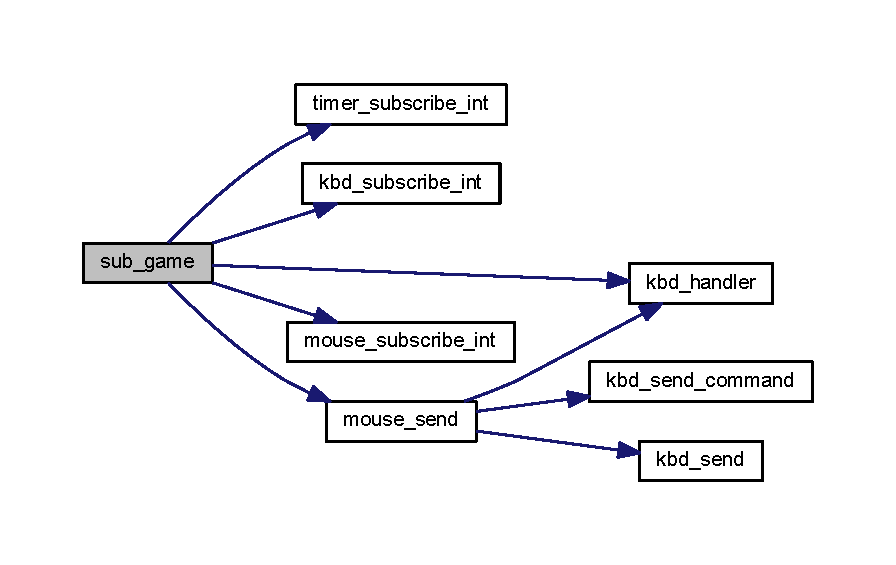
\includegraphics[width=350pt]{otherlabs_8h_a13393ae743886637e81723f6177e0ad1_cgraph}
\end{center}
\end{figure}
\hypertarget{otherlabs_8h_ab6fadc501bcb3a2a8d22f32c53a7e2bb}{}\label{otherlabs_8h_ab6fadc501bcb3a2a8d22f32c53a7e2bb} 
\index{otherlabs.\+h@{otherlabs.\+h}!timer\+\_\+subscribe\+\_\+int@{timer\+\_\+subscribe\+\_\+int}}
\index{timer\+\_\+subscribe\+\_\+int@{timer\+\_\+subscribe\+\_\+int}!otherlabs.\+h@{otherlabs.\+h}}
\subsubsection{\texorpdfstring{timer\+\_\+subscribe\+\_\+int()}{timer\_subscribe\_int()}}
{\footnotesize\ttfamily int timer\+\_\+subscribe\+\_\+int (\begin{DoxyParamCaption}\item[{\hyperlink{structgame__t}{game\+\_\+t} $\ast$}]{game1 }\end{DoxyParamCaption})}



Subscribes and enables Timer 0 interrupts. 

\begin{DoxyReturn}{Returns}
Returns bit order in interrupt mask; negative value on failure 
\end{DoxyReturn}
\hypertarget{otherlabs_8h_ae0888c4f8f20af35339447b3f228b884}{}\label{otherlabs_8h_ae0888c4f8f20af35339447b3f228b884} 
\index{otherlabs.\+h@{otherlabs.\+h}!timer\+\_\+unsubscribe\+\_\+int@{timer\+\_\+unsubscribe\+\_\+int}}
\index{timer\+\_\+unsubscribe\+\_\+int@{timer\+\_\+unsubscribe\+\_\+int}!otherlabs.\+h@{otherlabs.\+h}}
\subsubsection{\texorpdfstring{timer\+\_\+unsubscribe\+\_\+int()}{timer\_unsubscribe\_int()}}
{\footnotesize\ttfamily int timer\+\_\+unsubscribe\+\_\+int (\begin{DoxyParamCaption}\item[{\hyperlink{structgame__t}{game\+\_\+t} $\ast$}]{game1 }\end{DoxyParamCaption})}



Unsubscribes Timer 0 interrupts. 

\begin{DoxyReturn}{Returns}
Return 0 upon success and non-\/zero otherwise 
\end{DoxyReturn}
\hypertarget{otherlabs_8h_aeda1f986abc84e2fffa1c47aff4c4ad7}{}\label{otherlabs_8h_aeda1f986abc84e2fffa1c47aff4c4ad7} 
\index{otherlabs.\+h@{otherlabs.\+h}!unsub\+\_\+game@{unsub\+\_\+game}}
\index{unsub\+\_\+game@{unsub\+\_\+game}!otherlabs.\+h@{otherlabs.\+h}}
\subsubsection{\texorpdfstring{unsub\+\_\+game()}{unsub\_game()}}
{\footnotesize\ttfamily int unsub\+\_\+game (\begin{DoxyParamCaption}\item[{\hyperlink{structgame__t}{game\+\_\+t} $\ast$}]{game1 }\end{DoxyParamCaption})}



Unsubscribe Handler. 

Calls the Timer 0, Keyboard and Mouse interrupts unsubscription functions

\begin{DoxyReturn}{Returns}
Return 0 upon success and non-\/zero otherwise 
\end{DoxyReturn}
Here is the call graph for this function\+:
\nopagebreak
\begin{figure}[H]
\begin{center}
\leavevmode
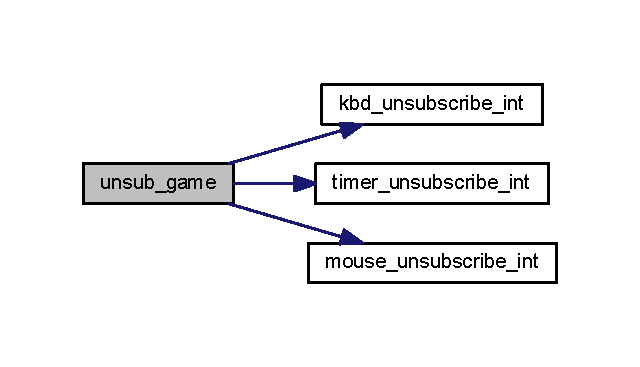
\includegraphics[width=307pt]{otherlabs_8h_aeda1f986abc84e2fffa1c47aff4c4ad7_cgraph}
\end{center}
\end{figure}

\hypertarget{read__bitmap_8c}{}\section{C\+:/\+Users/jnuno/\+Desktop/src/read\+\_\+bitmap.c File Reference}
\label{read__bitmap_8c}\index{C\+:/\+Users/jnuno/\+Desktop/src/read\+\_\+bitmap.\+c@{C\+:/\+Users/jnuno/\+Desktop/src/read\+\_\+bitmap.\+c}}
{\ttfamily \#include \char`\"{}read\+\_\+bitmap.\+h\char`\"{}}\newline
{\ttfamily \#include \char`\"{}stdio.\+h\char`\"{}}\newline
{\ttfamily \#include \char`\"{}video\+\_\+gr.\+h\char`\"{}}\newline
{\ttfamily \#include \char`\"{}tools.\+h\char`\"{}}\newline
Include dependency graph for read\+\_\+bitmap.\+c\+:
\nopagebreak
\begin{figure}[H]
\begin{center}
\leavevmode
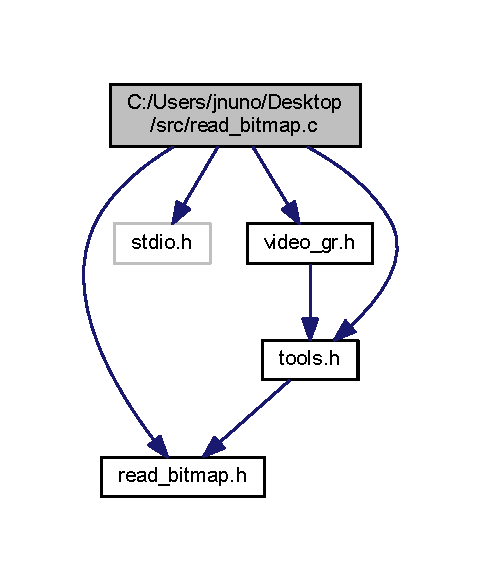
\includegraphics[width=231pt]{read__bitmap_8c__incl}
\end{center}
\end{figure}
\subsection*{Functions}
\begin{DoxyCompactItemize}
\item 
const char $\ast$ \hyperlink{group___bitmap_ga0dd46e75260201b6cd8211299bf9e703}{get\+Image\+Path} (const char $\ast$image)
\item 
\hyperlink{struct_bitmap}{Bitmap} $\ast$ \hyperlink{group___bitmap_ga3506880ffd407c36eb8aaddd2c1606d2}{load\+Bitmap} (const char $\ast$filename)
\begin{DoxyCompactList}\small\item\em Loads a bmp image. \end{DoxyCompactList}\item 
void \hyperlink{group___bitmap_gafe3e5be36ca808fa1383387b7943aa10}{draw\+Bitmap} (\hyperlink{struct_bitmap}{Bitmap} $\ast$bmp, int x, int y, int doublebf)
\begin{DoxyCompactList}\small\item\em Draws an unscaled, unrotated bitmap at the given position. \end{DoxyCompactList}\item 
void \hyperlink{group___bitmap_ga08c1d4f4fff81df260d979ea8fc1aa61}{delete\+Bitmap} (\hyperlink{struct_bitmap}{Bitmap} $\ast$bmp)
\begin{DoxyCompactList}\small\item\em Destroys the given bitmap, freeing all resources used by it. \end{DoxyCompactList}\end{DoxyCompactItemize}

\hypertarget{read__bitmap_8h}{}\section{C\+:/\+Users/jnuno/\+Desktop/src/read\+\_\+bitmap.h File Reference}
\label{read__bitmap_8h}\index{C\+:/\+Users/jnuno/\+Desktop/src/read\+\_\+bitmap.\+h@{C\+:/\+Users/jnuno/\+Desktop/src/read\+\_\+bitmap.\+h}}
This graph shows which files directly or indirectly include this file\+:
\nopagebreak
\begin{figure}[H]
\begin{center}
\leavevmode
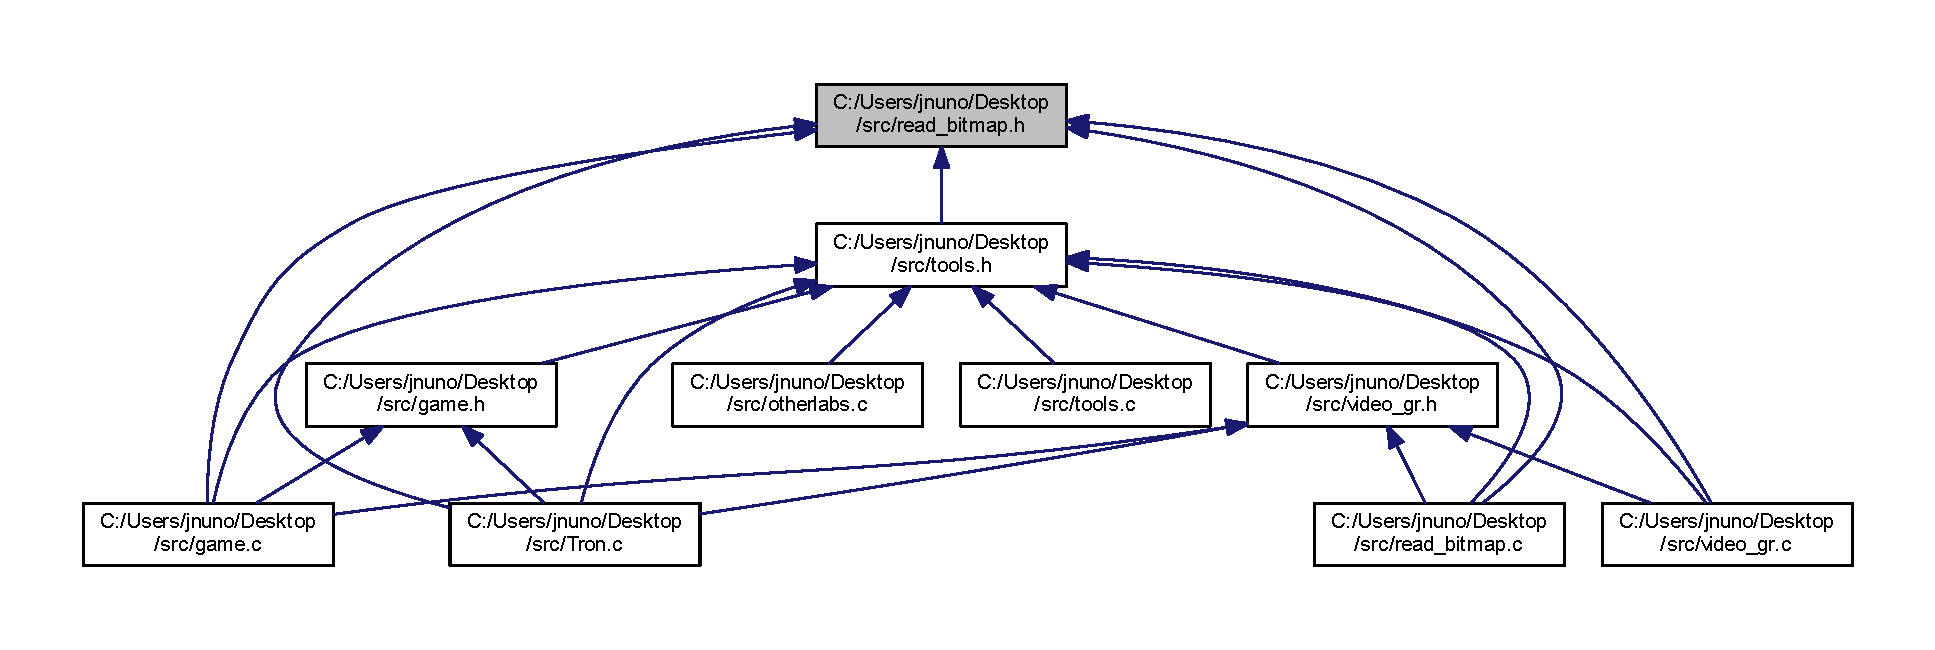
\includegraphics[width=350pt]{read__bitmap_8h__dep__incl}
\end{center}
\end{figure}
\subsection*{Data Structures}
\begin{DoxyCompactItemize}
\item 
struct \hyperlink{struct_bitmap_file_header}{Bitmap\+File\+Header}
\item 
struct \hyperlink{struct_bitmap_info_header}{Bitmap\+Info\+Header}
\item 
struct \hyperlink{struct_bitmap}{Bitmap}
\begin{DoxyCompactList}\small\item\em Represents a \hyperlink{struct_bitmap}{Bitmap}. \end{DoxyCompactList}\end{DoxyCompactItemize}
\subsection*{Functions}
\begin{DoxyCompactItemize}
\item 
const char $\ast$ \hyperlink{group___bitmap_ga0dd46e75260201b6cd8211299bf9e703}{get\+Image\+Path} (const char $\ast$image)
\item 
\hyperlink{struct_bitmap}{Bitmap} $\ast$ \hyperlink{group___bitmap_ga3506880ffd407c36eb8aaddd2c1606d2}{load\+Bitmap} (const char $\ast$filename)
\begin{DoxyCompactList}\small\item\em Loads a bmp image. \end{DoxyCompactList}\item 
void \hyperlink{group___bitmap_gafe3e5be36ca808fa1383387b7943aa10}{draw\+Bitmap} (\hyperlink{struct_bitmap}{Bitmap} $\ast$bitmap, int x, int y, int doublebf)
\begin{DoxyCompactList}\small\item\em Draws an unscaled, unrotated bitmap at the given position. \end{DoxyCompactList}\item 
void \hyperlink{group___bitmap_ga08c1d4f4fff81df260d979ea8fc1aa61}{delete\+Bitmap} (\hyperlink{struct_bitmap}{Bitmap} $\ast$bmp)
\begin{DoxyCompactList}\small\item\em Destroys the given bitmap, freeing all resources used by it. \end{DoxyCompactList}\end{DoxyCompactItemize}

\hypertarget{tools_8c}{}\section{C\+:/\+Users/jnuno/\+Desktop/src/tools.c File Reference}
\label{tools_8c}\index{C\+:/\+Users/jnuno/\+Desktop/src/tools.\+c@{C\+:/\+Users/jnuno/\+Desktop/src/tools.\+c}}
{\ttfamily \#include \char`\"{}tools.\+h\char`\"{}}\newline
Include dependency graph for tools.\+c\+:
\nopagebreak
\begin{figure}[H]
\begin{center}
\leavevmode
\includegraphics[width=200pt]{tools_8c__incl}
\end{center}
\end{figure}
\subsection*{Functions}
\begin{DoxyCompactItemize}
\item 
int \hyperlink{group__colors_ga8ac8469511c64983e8f0a678a14f0e36}{rgb} (unsigned char r, unsigned char g, unsigned char b)
\begin{DoxyCompactList}\small\item\em Calculates a color in R\+BG 5\+:6\+:5. \end{DoxyCompactList}\item 
void \hyperlink{group___game_ga97a9584ff1d8b78ede18e32bf5a7bd50}{init\+\_\+mouse} (\hyperlink{structgame__t}{game\+\_\+t} $\ast$game1)
\begin{DoxyCompactList}\small\item\em Initiates the mouse. \end{DoxyCompactList}\item 
int \hyperlink{group___game_ga1ebb9b5b5ce215ca81c1ca22526d935a}{init\+\_\+players} (unsigned int num\+\_\+players, \hyperlink{structgame__t}{game\+\_\+t} $\ast$game1)
\begin{DoxyCompactList}\small\item\em Initiates the players. \end{DoxyCompactList}\item 
void \hyperlink{group___game_ga1904435b0a61ef11d90bec5376eb6398}{draw\+\_\+board} (unsigned int num\+\_\+players, \hyperlink{structgame__t}{game\+\_\+t} $\ast$game1)
\begin{DoxyCompactList}\small\item\em Draws the background. \end{DoxyCompactList}\end{DoxyCompactItemize}

\hypertarget{tools_8h}{}\section{C\+:/\+Users/jnuno/\+Desktop/src/tools.h File Reference}
\label{tools_8h}\index{C\+:/\+Users/jnuno/\+Desktop/src/tools.\+h@{C\+:/\+Users/jnuno/\+Desktop/src/tools.\+h}}
{\ttfamily \#include \char`\"{}read\+\_\+bitmap.\+h\char`\"{}}\newline
Include dependency graph for tools.\+h\+:
\nopagebreak
\begin{figure}[H]
\begin{center}
\leavevmode
\includegraphics[width=200pt]{tools_8h__incl}
\end{center}
\end{figure}
This graph shows which files directly or indirectly include this file\+:
\nopagebreak
\begin{figure}[H]
\begin{center}
\leavevmode
\includegraphics[width=350pt]{tools_8h__dep__incl}
\end{center}
\end{figure}
\subsection*{Data Structures}
\begin{DoxyCompactItemize}
\item 
struct \hyperlink{structplayer__t}{player\+\_\+t}
\item 
struct \hyperlink{structmouse__t}{mouse\+\_\+t}
\item 
struct \hyperlink{structboard__t}{board\+\_\+t}
\item 
struct \hyperlink{structgame__t}{game\+\_\+t}
\end{DoxyCompactItemize}
\subsection*{Macros}
\begin{DoxyCompactItemize}
\item 
\#define \hyperlink{tools_8h_a3a8ea58898cb58fc96013383d39f482c}{B\+IT}(n)~(0x01$<$$<$(n))
\item 
\#define \hyperlink{group__i8254_ga30bf84c312af248cb81bb224e09f9ba8}{T\+I\+M\+E\+R0\+\_\+\+I\+RQ}~0
\begin{DoxyCompactList}\small\item\em Timer 0 I\+RQ line. \end{DoxyCompactList}\item 
\#define \hyperlink{group__i8254_gacc9ff9df4a9674a1ce9ba08fc4a4679e}{T\+I\+M\+E\+R\+\_\+0}~0x40
\begin{DoxyCompactList}\small\item\em Timer 0 count register. \end{DoxyCompactList}\item 
\#define \hyperlink{group__i8254_ga282832448fb0281ef53d243c1cd48491}{T\+I\+M\+E\+R\+\_\+\+C\+T\+RL}~0x43
\begin{DoxyCompactList}\small\item\em Control register. \end{DoxyCompactList}\item 
\#define \hyperlink{group__i8254_ga6a4822642d40c248435692324a818010}{T\+I\+M\+E\+R\+\_\+\+S\+E\+L0}~0x00
\begin{DoxyCompactList}\small\item\em Control Word for Timer 0. \end{DoxyCompactList}\item 
\#define \hyperlink{group__i8254_ga4c2eecbfb96744a9c2af71dba75ecb18}{T\+I\+M\+E\+R\+\_\+\+R\+B\+\_\+\+C\+MD}~(\hyperlink{tools_8h_a3a8ea58898cb58fc96013383d39f482c}{B\+IT}(7)$\vert$\hyperlink{tools_8h_a3a8ea58898cb58fc96013383d39f482c}{B\+IT}(6))
\begin{DoxyCompactList}\small\item\em Read Back Command. \end{DoxyCompactList}\item 
\#define \hyperlink{group__i8254_gaa8b3f7a4eeaccbeb4e42a2ca6a9d0cd8}{T\+M0\+\_\+\+I\+R\+Q\+S\+ET}~0
\begin{DoxyCompactList}\small\item\em Timer 0 irq\+\_\+set for bitmask. \end{DoxyCompactList}\item 
\#define \hyperlink{group__i8254_ga1a522aa19bcb695a9df30032a893bee3}{D\+E\+L\+A\+Y\+\_\+\+US}~20000
\item 
\#define \hyperlink{group__i8042_gae36fc325bc821e866e90d0e66f9cc168}{K\+B\+\_\+\+I\+RQ}~1
\item 
\#define \hyperlink{group__i8042_ga2d17911b50c0aeebb2e3325c5b36d4f2}{K\+E\+Y\+B\+O\+A\+R\+D\+\_\+\+I\+RQ}~1
\item 
\#define \hyperlink{group__i8042_ga923231d2e45aaea2dbab3532b06c2311}{S\+T\+A\+T\+U\+S\+\_\+\+P\+O\+RT}~0x64
\begin{DoxyCompactList}\small\item\em Status Port register. \end{DoxyCompactList}\item 
\#define \hyperlink{group__i8042_gaeff3162e464a9081f73e3765f199d7c1}{K\+B\+D\+\_\+\+O\+U\+T\+\_\+\+B\+UF}~0x60
\begin{DoxyCompactList}\small\item\em Output Buffer register. \end{DoxyCompactList}\item 
\#define \hyperlink{group__i8042_gae1f561b740c8aed366ab0f6618e391f3}{K\+B\+D\+\_\+\+I\+N\+P\+T\+\_\+\+B\+UF}~0x64
\begin{DoxyCompactList}\small\item\em Input Buffer register. \end{DoxyCompactList}\item 
\#define \hyperlink{group__i8042_ga45967c9e25447ba853cf6fb4ac545fe6}{O\+BF}~\hyperlink{tools_8h_a3a8ea58898cb58fc96013383d39f482c}{B\+IT}(0)
\begin{DoxyCompactList}\small\item\em Control Word for Output Buffer Full. \end{DoxyCompactList}\item 
\#define \hyperlink{group__i8042_ga3c48b10907056351582baf9f6478598e}{I\+BF}~\hyperlink{tools_8h_a3a8ea58898cb58fc96013383d39f482c}{B\+IT}(1)
\begin{DoxyCompactList}\small\item\em Control Word for Input Buffer Full. \end{DoxyCompactList}\item 
\#define \hyperlink{group__i8042_gab427e6926fcc47eb1c02c1f78162b6f6}{T\+W\+O\+\_\+\+B\+Y\+T\+ES}~0x\+E0
\begin{DoxyCompactList}\small\item\em Control Word for 2 bytes scancodes. \end{DoxyCompactList}\item 
\#define \hyperlink{group__i8042_ga307ab71673e26ec42b28a3bca05d4cb5}{P\+A\+R\+\_\+\+E\+RR}~\hyperlink{tools_8h_a3a8ea58898cb58fc96013383d39f482c}{B\+IT}(7)
\item 
\#define \hyperlink{group__i8042_gad16f61e2bf70f6c7685e826224ed177f}{T\+O\+\_\+\+E\+RR}~\hyperlink{tools_8h_a3a8ea58898cb58fc96013383d39f482c}{B\+IT}(6)
\item 
\#define \hyperlink{group__mouse_gaf5b75ec709ee94625a79692c87cc7b7a}{M\+O\+U\+S\+E\+\_\+\+S\+E\+ND}~0x\+D4
\item 
\#define \hyperlink{group__mouse_ga7c88f18c3c70a4afefba1a8f772c7036}{M\+O\+U\+S\+E\+\_\+\+E\+NB}~0x\+F4
\item 
\#define \hyperlink{group__mouse_ga199b8aec1af091ef16f1483d4aa4b345}{M\+O\+U\+S\+E\+\_\+\+C\+O\+NF}~0x\+E9
\item 
\#define \hyperlink{group__mouse_ga0349a2901e942eb948442081d0aedc96}{K\+B\+\_\+\+A\+CK}~0x\+FA
\item 
\#define \hyperlink{group__mouse_ga6d57c7927a10f638c83046b52c8caac9}{K\+B\+C\+\_\+\+C\+M\+D\+\_\+\+R\+EG}~0x64
\item 
\#define \hyperlink{group__mouse_ga95745d05db38ca00871939ef479aeb56}{K\+B\+D\+\_\+\+D\+A\+T\+A\+\_\+\+B\+UF}~0x60
\item 
\#define \hyperlink{group__mouse_ga85964cb90343bb1a029b1d1b4229f910}{M\+O\+U\+S\+E\+\_\+\+I\+RQ}~12
\item 
\#define \hyperlink{group__mouse_ga0e16a37e9b19ac48591b3899fc7580ea}{G\+R\+\_\+\+M\+O\+DE}~0x11A
\item 
\#define \hyperlink{group__mouse_ga327c2a8d523460fa45ca05492a003d56}{H\+R\+ES}~1280
\item 
\#define \hyperlink{group__mouse_gacf2cfe6990fa35811b2a0b2f4b77bbdb}{V\+R\+ES}~1024
\item 
\#define \hyperlink{group__mouse_gaee3d3431c33559daa9472d32dbaa76cc}{X\+L\+L\+I\+M\+IT}~50
\item 
\#define \hyperlink{group__mouse_gaccc38829dd9a253af163a2e05124d239}{X\+R\+L\+I\+M\+IT}~1250
\item 
\#define \hyperlink{group__mouse_ga7afa9a9c3f789856869ae1a766cc917f}{Y\+U\+L\+I\+M\+IT}~200
\item 
\#define \hyperlink{group__mouse_gaec42b751ff3806b4f7102f7564fdf34d}{Y\+D\+L\+I\+M\+IT}~1000
\item 
\#define \hyperlink{group__mouse_ga4a627ba1f66cbd6c5de585d5002ebe96}{M\+E\+N\+U1U}~347
\item 
\#define \hyperlink{group__mouse_gabc4d39c53c1b122b66301e6d91fec329}{M\+E\+N\+U1D}~435
\item 
\#define \hyperlink{group__mouse_gaf46df8ae7d292764e0bd733b5a69fa97}{M\+E\+N\+U1L}~221
\item 
\#define \hyperlink{group__mouse_ga280f604342f10e7da8eb79e5364f134e}{M\+E\+N\+U1R}~578
\item 
\#define \hyperlink{group__mouse_gad344b0e0080be13940f676b3fb921604}{M\+E\+N\+U2U}~347
\item 
\#define \hyperlink{group__mouse_ga5f1d419164811a353a3fb91ab934b008}{M\+E\+N\+U2D}~435
\item 
\#define \hyperlink{group__mouse_gaf9c31d922032006354f0f94d0dbfba86}{M\+E\+N\+U2L}~715
\item 
\#define \hyperlink{group__mouse_ga9ba96b159609610c99e1e56ae532ce2e}{M\+E\+N\+U2R}~1071
\item 
\#define \hyperlink{group__mouse_ga58d0568b55739b936c55a4cd70642273}{M\+E\+N\+U3U}~526
\item 
\#define \hyperlink{group__mouse_ga1bf711f126b31c1e93c4273139dda3d5}{M\+E\+N\+U3D}~614
\item 
\#define \hyperlink{group__mouse_ga261b94752f05faaea72b95f89fb4eaae}{M\+E\+N\+U3L}~221
\item 
\#define \hyperlink{group__mouse_ga4b14d3a27693996fda99359c830d3d0f}{M\+E\+N\+U3R}~578
\item 
\#define \hyperlink{group__mouse_gaaa91c726154bcb919ad804280ef7b402}{M\+E\+N\+U4U}~526
\item 
\#define \hyperlink{group__mouse_ga49904fe1a8177385da2f91915bd5e123}{M\+E\+N\+U4D}~614
\item 
\#define \hyperlink{group__mouse_ga455cfaa20c07781a8036731bd000b7f4}{M\+E\+N\+U4L}~715
\item 
\#define \hyperlink{group__mouse_ga1234a94f05b8102de0c93698aaf08085}{M\+E\+N\+U4R}~1071
\item 
\#define \hyperlink{group__colors_gabc93b0adf636edc12e8e9e0489429972}{O\+R\+A\+N\+G\+E1}~\hyperlink{group__colors_ga8ac8469511c64983e8f0a678a14f0e36}{rgb}(223,116,12);
\item 
\#define \hyperlink{group__colors_ga8ac45568d18ed08eb1ff4e9355110f6e}{O\+R\+A\+N\+G\+E2}~\hyperlink{group__colors_ga8ac8469511c64983e8f0a678a14f0e36}{rgb}(255,230,77);
\item 
\#define \hyperlink{group__colors_ga30100d62cd1f80d21430872e1be9c543}{B\+L\+U\+E1}~\hyperlink{group__colors_ga8ac8469511c64983e8f0a678a14f0e36}{rgb}(111,195,223);
\item 
\#define \hyperlink{group__colors_ga741d26513518e80fdef905dc6f209fc8}{B\+L\+U\+E2}~\hyperlink{group__colors_ga8ac8469511c64983e8f0a678a14f0e36}{rgb}(230,255,255);
\item 
\#define \hyperlink{group__colors_ga343686a86fcf4e10a82059b078b1b7d0}{G\+R\+E\+E\+N1}~\hyperlink{group__colors_ga8ac8469511c64983e8f0a678a14f0e36}{rgb}(8,254,20);
\item 
\#define \hyperlink{group__colors_ga0514cf5f3dd5549be9c93c6ec588dbd5}{P\+I\+N\+K1}~\hyperlink{group__colors_ga8ac8469511c64983e8f0a678a14f0e36}{rgb}(255,54,155);
\item 
\#define \hyperlink{group__colors_ga87b537f5fa5c109d3c05c13d6b18f382}{W\+H\+I\+TE}~\hyperlink{group__colors_ga8ac8469511c64983e8f0a678a14f0e36}{rgb}(255,255,255);
\item 
\#define \hyperlink{group__colors_ga7b3b25cba33b07c303f3060fe41887f6}{B\+L\+A\+CK}~\hyperlink{group__colors_ga8ac8469511c64983e8f0a678a14f0e36}{rgb}(0,0,0);
\item 
\#define \hyperlink{group__scancodes_ga343f44cb034d2d2ff3438b3d45dcde1f}{E\+S\+C\+\_\+\+B\+R\+E\+AK}~0x81
\item 
\#define \hyperlink{group__scancodes_ga168fd0a54619731c76c386a7f1bde2b1}{E\+S\+C\+\_\+\+M\+A\+KE}~0x01
\item 
\#define \hyperlink{group__scancodes_ga95d6e4b61bac77469ecc47b205709af6}{S\+P\+A\+C\+E\+\_\+\+B\+R\+E\+AK}~0x\+B9
\item 
\#define \hyperlink{group__scancodes_ga0f76fe84c649e8cf3a4114d0d9bf085a}{A\+\_\+\+M\+A\+KE}~0x1E
\item 
\#define \hyperlink{group__scancodes_ga05826112c5acf959ee58dcacd8e9d065}{A\+\_\+\+B\+R\+E\+AK}~0x9E
\item 
\#define \hyperlink{group__scancodes_gac822a3953d90207e64b58f480454a8d8}{W\+\_\+\+M\+A\+KE}~0x11
\item 
\#define \hyperlink{group__scancodes_ga32d11f9abffe8bb3df11feef5ca5213d}{W\+\_\+\+B\+R\+E\+AK}~0x91
\item 
\#define \hyperlink{group__scancodes_gac2c2b345d42f2a5b5a028028eb8c5680}{S\+\_\+\+M\+A\+KE}~0x1F
\item 
\#define \hyperlink{group__scancodes_ga85b3c65b8b6c952e08c252e9737b74f9}{S\+\_\+\+B\+R\+E\+AK}~0x9F
\item 
\#define \hyperlink{group__scancodes_ga629b0c93e278a4bf1e1678af58fbea95}{D\+\_\+\+M\+A\+KE}~0x20
\item 
\#define \hyperlink{group__scancodes_gad2db9242348c43c781cc14746060470b}{D\+\_\+\+B\+R\+E\+AK}~0x\+A0
\item 
\#define \hyperlink{group__scancodes_ga4c8f4d4420f9ec7ef30de25264efa68a}{U\+A\+R\+R\+O\+W\+\_\+\+M\+A\+KE}~0x\+E048
\item 
\#define \hyperlink{group__scancodes_ga9ab3dee73aef06dca9ef9b37b818acb2}{U\+A\+R\+R\+O\+W\+\_\+\+B\+R\+E\+AK}~0x\+E0\+C8
\item 
\#define \hyperlink{group__scancodes_gad9509ca6995b9d5ca117d0ea8004cfef}{L\+A\+R\+R\+O\+W\+\_\+\+M\+A\+KE}~0x\+E04B
\item 
\#define \hyperlink{group__scancodes_ga335ac9047c7a6d0c8631014766f96484}{L\+A\+R\+R\+O\+W\+\_\+\+B\+R\+E\+AK}~0x\+E0\+CB
\item 
\#define \hyperlink{group__scancodes_ga5e0594973062eb7d381ee43ff19a0369}{D\+A\+R\+R\+O\+W\+\_\+\+M\+A\+KE}~0x\+E050
\item 
\#define \hyperlink{group__scancodes_ga02742462a869b87ad2a34d8bc6a3fe58}{D\+A\+R\+R\+O\+W\+\_\+\+B\+R\+E\+AK}~0x\+E0\+D0
\item 
\#define \hyperlink{group__scancodes_ga365f3fec5881bea630c70f2c1098263f}{R\+A\+R\+R\+O\+W\+\_\+\+M\+A\+KE}~0x\+E04D
\item 
\#define \hyperlink{group__scancodes_ga9dd5fb482207f2c4f76696b443f76020}{R\+A\+R\+R\+O\+W\+\_\+\+B\+R\+E\+AK}~0x\+E0\+CD
\item 
\#define \hyperlink{group__scancodes_gaa7a13a11c6b4a4b22cc8c2dd5cca7a95}{B\+\_\+\+M\+A\+KE}~0x30
\item 
\#define \hyperlink{group__scancodes_ga357a1debdc4027db65b315366e9019dd}{M\+\_\+\+M\+A\+KE}~0x32
\item 
\#define \hyperlink{group__scancodes_ga124c06c60ba6b840260900c1fa975163}{I\+\_\+\+M\+A\+KE}~0x17
\item 
\#define \hyperlink{group__scancodes_gace8d1d82b15ad6363a0026421bc87fd6}{P\+\_\+\+M\+A\+KE}~0x19
\item 
\#define \hyperlink{group__scancodes_ga1921ae02c4c330897f27c61827f24a4c}{N\+U\+M2\+\_\+\+B\+R\+E\+AK}~0x83
\item 
\#define \hyperlink{group__scancodes_ga2b19345612635fb7cc2774bf1d18bbcd}{N\+U\+M3\+\_\+\+B\+R\+E\+AK}~0x84
\item 
\#define \hyperlink{group__scancodes_ga10d66972ee092e45e01d18921164ef72}{N\+U\+M4\+\_\+\+B\+R\+E\+AK}~0x85
\end{DoxyCompactItemize}
\subsection*{Enumerations}
\begin{DoxyCompactItemize}
\item 
enum \hyperlink{group___game_gaa0aafed44fec19806d8f9ad834be1248}{state\+\_\+t} \{ \newline
\hyperlink{group___game_ggaa0aafed44fec19806d8f9ad834be1248adb45120aafd37a973140edee24708065}{L\+E\+FT}, 
\hyperlink{group___game_ggaa0aafed44fec19806d8f9ad834be1248aec8379af7490bb9eaaf579cf17876f38}{R\+I\+G\+HT}, 
\hyperlink{group___game_ggaa0aafed44fec19806d8f9ad834be1248aba595d8bca8bc5e67c37c0a9d89becfa}{UP}, 
\hyperlink{group___game_ggaa0aafed44fec19806d8f9ad834be1248a9b0b4a95b99523966e0e34ffdadac9da}{D\+O\+WN}, 
\newline
\hyperlink{group___game_ggaa0aafed44fec19806d8f9ad834be1248a679ee5320d66c8322e310daeb2ee99b8}{S\+T\+OP}
 \}
\item 
enum \hyperlink{group___game_ga4edce1ca040716922b6e4a79be4e414d}{game\+\_\+state\+\_\+t} \{ \newline
\hyperlink{group___game_gga4edce1ca040716922b6e4a79be4e414da4c40e60bc71a32b924ce1f08d57f9721}{M\+E\+NU}, 
\hyperlink{group___game_gga4edce1ca040716922b6e4a79be4e414da0cb1b2c6a7db1f1084886c98909a3f36}{I\+N\+IT}, 
\hyperlink{group___game_gga4edce1ca040716922b6e4a79be4e414daf095245f5cebc27a97a124345269fed8}{P\+L\+A\+Y\+I\+NG}, 
\hyperlink{group___game_gga4edce1ca040716922b6e4a79be4e414dad4bb05915de3c370d3a33d4f51389655}{P\+A\+U\+S\+ED}, 
\newline
\hyperlink{group___game_gga4edce1ca040716922b6e4a79be4e414dadbd1812bee789fbf3548cf79d3f2b400}{F\+I\+N\+I\+S\+H\+ED}, 
\hyperlink{group___game_gga4edce1ca040716922b6e4a79be4e414da76bdc8adfd6c6463ab269ff4c06be9b4}{Q\+U\+IT}
 \}
\item 
enum \hyperlink{group___game_gaabca14b349ba212174a00ffc1d2a2f31}{ev\+\_\+type\+\_\+t} \{ \hyperlink{group___game_ggaabca14b349ba212174a00ffc1d2a2f31a1a1b5730082d8a99750ec1442ef473b3}{K\+D\+O\+WN}, 
\hyperlink{group___game_ggaabca14b349ba212174a00ffc1d2a2f31a7811143a3a1f6274d18050dd91a6586e}{K\+UP}
 \}
\end{DoxyCompactItemize}
\subsection*{Functions}
\begin{DoxyCompactItemize}
\item 
int \hyperlink{group__colors_ga8ac8469511c64983e8f0a678a14f0e36}{rgb} (unsigned char r, unsigned char g, unsigned char b)
\begin{DoxyCompactList}\small\item\em Calculates a color in R\+BG 5\+:6\+:5. \end{DoxyCompactList}\item 
void \hyperlink{group___game_ga97a9584ff1d8b78ede18e32bf5a7bd50}{init\+\_\+mouse} (\hyperlink{structgame__t}{game\+\_\+t} $\ast$game1)
\begin{DoxyCompactList}\small\item\em Initiates the mouse. \end{DoxyCompactList}\item 
int \hyperlink{group___game_ga1ebb9b5b5ce215ca81c1ca22526d935a}{init\+\_\+players} (unsigned int num\+\_\+players, \hyperlink{structgame__t}{game\+\_\+t} $\ast$game1)
\begin{DoxyCompactList}\small\item\em Initiates the players. \end{DoxyCompactList}\item 
void \hyperlink{group___game_ga1904435b0a61ef11d90bec5376eb6398}{draw\+\_\+board} (unsigned int num\+\_\+players, \hyperlink{structgame__t}{game\+\_\+t} $\ast$game1)
\begin{DoxyCompactList}\small\item\em Draws the background. \end{DoxyCompactList}\end{DoxyCompactItemize}


\subsection{Macro Definition Documentation}
\hypertarget{tools_8h_a3a8ea58898cb58fc96013383d39f482c}{}\label{tools_8h_a3a8ea58898cb58fc96013383d39f482c} 
\index{tools.\+h@{tools.\+h}!B\+IT@{B\+IT}}
\index{B\+IT@{B\+IT}!tools.\+h@{tools.\+h}}
\subsubsection{\texorpdfstring{B\+IT}{BIT}}
{\footnotesize\ttfamily \#define B\+IT(\begin{DoxyParamCaption}\item[{}]{n }\end{DoxyParamCaption})~(0x01$<$$<$(n))}


\hypertarget{_tron_8c}{}\section{C\+:/\+Users/jnuno/\+Desktop/src/\+Tron.c File Reference}
\label{_tron_8c}\index{C\+:/\+Users/jnuno/\+Desktop/src/\+Tron.\+c@{C\+:/\+Users/jnuno/\+Desktop/src/\+Tron.\+c}}
{\ttfamily \#include \char`\"{}lmlib.\+h\char`\"{}}\newline
{\ttfamily \#include \char`\"{}vbe.\+h\char`\"{}}\newline
{\ttfamily \#include \char`\"{}video\+\_\+gr.\+h\char`\"{}}\newline
{\ttfamily \#include \char`\"{}game.\+h\char`\"{}}\newline
{\ttfamily \#include \char`\"{}otherlabs.\+h\char`\"{}}\newline
{\ttfamily \#include \char`\"{}tools.\+h\char`\"{}}\newline
{\ttfamily \#include \char`\"{}read\+\_\+bitmap.\+h\char`\"{}}\newline
{\ttfamily \#include $<$limits.\+h$>$}\newline
{\ttfamily \#include $<$string.\+h$>$}\newline
{\ttfamily \#include $<$errno.\+h$>$}\newline
Include dependency graph for Tron.\+c\+:
\nopagebreak
\begin{figure}[H]
\begin{center}
\leavevmode
\includegraphics[width=350pt]{_tron_8c__incl}
\end{center}
\end{figure}
\subsection*{Functions}
\begin{DoxyCompactItemize}
\item 
int \hyperlink{_tron_8c_a0ddf1224851353fc92bfbff6f499fa97}{main} (int argc, char $\ast$argv\mbox{[}$\,$\mbox{]})
\end{DoxyCompactItemize}


\subsection{Function Documentation}
\hypertarget{_tron_8c_a0ddf1224851353fc92bfbff6f499fa97}{}\label{_tron_8c_a0ddf1224851353fc92bfbff6f499fa97} 
\index{Tron.\+c@{Tron.\+c}!main@{main}}
\index{main@{main}!Tron.\+c@{Tron.\+c}}
\subsubsection{\texorpdfstring{main()}{main()}}
{\footnotesize\ttfamily int main (\begin{DoxyParamCaption}\item[{int}]{argc,  }\item[{char $\ast$}]{argv\mbox{[}$\,$\mbox{]} }\end{DoxyParamCaption})}

Video mode 0x11A -\/$>$ 1280x1024 16bit 5\+:6\+:5Here is the call graph for this function\+:
\nopagebreak
\begin{figure}[H]
\begin{center}
\leavevmode
\includegraphics[width=350pt]{_tron_8c_a0ddf1224851353fc92bfbff6f499fa97_cgraph}
\end{center}
\end{figure}

\hypertarget{vbe_8c}{}\section{C\+:/\+Users/jnuno/\+Desktop/src/vbe.c File Reference}
\label{vbe_8c}\index{C\+:/\+Users/jnuno/\+Desktop/src/vbe.\+c@{C\+:/\+Users/jnuno/\+Desktop/src/vbe.\+c}}
{\ttfamily \#include $<$minix/syslib.\+h$>$}\newline
{\ttfamily \#include $<$minix/drivers.\+h$>$}\newline
{\ttfamily \#include $<$machine/int86.\+h$>$}\newline
{\ttfamily \#include \char`\"{}vbe.\+h\char`\"{}}\newline
{\ttfamily \#include \char`\"{}lmlib.\+h\char`\"{}}\newline
Include dependency graph for vbe.\+c\+:
\nopagebreak
\begin{figure}[H]
\begin{center}
\leavevmode
\includegraphics[width=350pt]{vbe_8c__incl}
\end{center}
\end{figure}
\subsection*{Macros}
\begin{DoxyCompactItemize}
\item 
\#define \hyperlink{vbe_8c_a0007120a310d0ec70307f51f43eb81a3}{L\+I\+N\+E\+A\+R\+\_\+\+M\+O\+D\+E\+L\+\_\+\+B\+IT}~14
\item 
\#define \hyperlink{vbe_8c_a68b87c2339cb305d66b69b5551b96c73}{P\+B2\+B\+A\+SE}(x)~(((x) $>$$>$ 4) \& 0x0\+F000)
\item 
\#define \hyperlink{vbe_8c_a70c65ed4c6d71865daa96d31befb33fd}{P\+B2\+O\+FF}(x)~((x) \& 0x0\+F\+F\+F\+F)
\end{DoxyCompactItemize}
\subsection*{Functions}
\begin{DoxyCompactItemize}
\item 
int \hyperlink{group__vbe_ga4ef3234e41f2050bc094a22049b69e45}{vbe\+\_\+get\+\_\+mode\+\_\+info} (unsigned short mode, vbe\+\_\+mode\+\_\+info\+\_\+t $\ast$vmi\+\_\+p)
\begin{DoxyCompactList}\small\item\em Returns information on the input V\+BE mode, including screen dimensions, color depth and V\+R\+AM physical address. \end{DoxyCompactList}\item 
int \hyperlink{group__vbe_ga04ba27e16f8dc8fb472f6f57cf66538a}{vbe\+\_\+get\+\_\+controller\+\_\+info} (Vbe\+Info\+Block $\ast$vib\+\_\+p)
\end{DoxyCompactItemize}


\subsection{Macro Definition Documentation}
\hypertarget{vbe_8c_a0007120a310d0ec70307f51f43eb81a3}{}\label{vbe_8c_a0007120a310d0ec70307f51f43eb81a3} 
\index{vbe.\+c@{vbe.\+c}!L\+I\+N\+E\+A\+R\+\_\+\+M\+O\+D\+E\+L\+\_\+\+B\+IT@{L\+I\+N\+E\+A\+R\+\_\+\+M\+O\+D\+E\+L\+\_\+\+B\+IT}}
\index{L\+I\+N\+E\+A\+R\+\_\+\+M\+O\+D\+E\+L\+\_\+\+B\+IT@{L\+I\+N\+E\+A\+R\+\_\+\+M\+O\+D\+E\+L\+\_\+\+B\+IT}!vbe.\+c@{vbe.\+c}}
\subsubsection{\texorpdfstring{L\+I\+N\+E\+A\+R\+\_\+\+M\+O\+D\+E\+L\+\_\+\+B\+IT}{LINEAR\_MODEL\_BIT}}
{\footnotesize\ttfamily \#define L\+I\+N\+E\+A\+R\+\_\+\+M\+O\+D\+E\+L\+\_\+\+B\+IT~14}

\hypertarget{vbe_8c_a68b87c2339cb305d66b69b5551b96c73}{}\label{vbe_8c_a68b87c2339cb305d66b69b5551b96c73} 
\index{vbe.\+c@{vbe.\+c}!P\+B2\+B\+A\+SE@{P\+B2\+B\+A\+SE}}
\index{P\+B2\+B\+A\+SE@{P\+B2\+B\+A\+SE}!vbe.\+c@{vbe.\+c}}
\subsubsection{\texorpdfstring{P\+B2\+B\+A\+SE}{PB2BASE}}
{\footnotesize\ttfamily \#define P\+B2\+B\+A\+SE(\begin{DoxyParamCaption}\item[{}]{x }\end{DoxyParamCaption})~(((x) $>$$>$ 4) \& 0x0\+F000)}

\hypertarget{vbe_8c_a70c65ed4c6d71865daa96d31befb33fd}{}\label{vbe_8c_a70c65ed4c6d71865daa96d31befb33fd} 
\index{vbe.\+c@{vbe.\+c}!P\+B2\+O\+FF@{P\+B2\+O\+FF}}
\index{P\+B2\+O\+FF@{P\+B2\+O\+FF}!vbe.\+c@{vbe.\+c}}
\subsubsection{\texorpdfstring{P\+B2\+O\+FF}{PB2OFF}}
{\footnotesize\ttfamily \#define P\+B2\+O\+FF(\begin{DoxyParamCaption}\item[{}]{x }\end{DoxyParamCaption})~((x) \& 0x0\+F\+F\+F\+F)}


\hypertarget{vbe_8h}{}\section{C\+:/\+Users/jnuno/\+Desktop/src/vbe.h File Reference}
\label{vbe_8h}\index{C\+:/\+Users/jnuno/\+Desktop/src/vbe.\+h@{C\+:/\+Users/jnuno/\+Desktop/src/vbe.\+h}}
{\ttfamily \#include $<$stdint.\+h$>$}\newline
Include dependency graph for vbe.\+h\+:
\nopagebreak
\begin{figure}[H]
\begin{center}
\leavevmode
\includegraphics[width=200pt]{vbe_8h__incl}
\end{center}
\end{figure}
This graph shows which files directly or indirectly include this file\+:
\nopagebreak
\begin{figure}[H]
\begin{center}
\leavevmode
\includegraphics[width=350pt]{vbe_8h__dep__incl}
\end{center}
\end{figure}
\subsection*{Data Structures}
\begin{DoxyCompactItemize}
\item 
struct \hyperlink{struct____attribute____}{\+\_\+\+\_\+attribute\+\_\+\+\_\+}
\item 
struct \hyperlink{struct____attribute____}{\+\_\+\+\_\+attribute\+\_\+\+\_\+}
\end{DoxyCompactItemize}
\subsection*{Functions}
\begin{DoxyCompactItemize}
\item 
int \hyperlink{group__vbe_ga4ef3234e41f2050bc094a22049b69e45}{vbe\+\_\+get\+\_\+mode\+\_\+info} (unsigned short mode, vbe\+\_\+mode\+\_\+info\+\_\+t $\ast$vmi\+\_\+p)
\begin{DoxyCompactList}\small\item\em Returns information on the input V\+BE mode, including screen dimensions, color depth and V\+R\+AM physical address. \end{DoxyCompactList}\item 
int \hyperlink{group__vbe_ga04ba27e16f8dc8fb472f6f57cf66538a}{vbe\+\_\+get\+\_\+controller\+\_\+info} (Vbe\+Info\+Block $\ast$vib\+\_\+p)
\end{DoxyCompactItemize}

\hypertarget{video__gr_8c}{}\section{C\+:/\+Users/jnuno/\+Desktop/src/video\+\_\+gr.c File Reference}
\label{video__gr_8c}\index{C\+:/\+Users/jnuno/\+Desktop/src/video\+\_\+gr.\+c@{C\+:/\+Users/jnuno/\+Desktop/src/video\+\_\+gr.\+c}}
{\ttfamily \#include $<$minix/syslib.\+h$>$}\newline
{\ttfamily \#include $<$minix/drivers.\+h$>$}\newline
{\ttfamily \#include $<$machine/int86.\+h$>$}\newline
{\ttfamily \#include $<$sys/mman.\+h$>$}\newline
{\ttfamily \#include $<$sys/types.\+h$>$}\newline
{\ttfamily \#include \char`\"{}video\+\_\+gr.\+h\char`\"{}}\newline
{\ttfamily \#include \char`\"{}vbe.\+h\char`\"{}}\newline
{\ttfamily \#include \char`\"{}read\+\_\+bitmap.\+h\char`\"{}}\newline
{\ttfamily \#include \char`\"{}tools.\+h\char`\"{}}\newline
Include dependency graph for video\+\_\+gr.\+c\+:
\nopagebreak
\begin{figure}[H]
\begin{center}
\leavevmode
\includegraphics[width=350pt]{video__gr_8c__incl}
\end{center}
\end{figure}
\subsection*{Functions}
\begin{DoxyCompactItemize}
\item 
void $\ast$ \hyperlink{group__video__gr_gacef21667c79365d57a084bed994c2189}{vg\+\_\+init} (unsigned short mode)
\begin{DoxyCompactList}\small\item\em Initializes the video module in graphics mode. \end{DoxyCompactList}\item 
void $\ast$ \hyperlink{group__video__gr_ga5ad1cc85a8dce3ce1a7d3e90e6ff88d3}{vg\+\_\+vd\+\_\+get\+\_\+vmem} ()
\begin{DoxyCompactList}\small\item\em Returns the Address of video\+\_\+mem. \end{DoxyCompactList}\item 
void $\ast$ \hyperlink{group__video__gr_ga3a176fda764c03218b5c20797f8b255e}{vg\+\_\+vd\+\_\+get\+\_\+vbuff} ()
\begin{DoxyCompactList}\small\item\em Returns the Address of the double buffer. \end{DoxyCompactList}\item 
void \hyperlink{group__video__gr_gab42788264b43ce014d787544fc12fdc6}{paint\+\_\+buff} ()
\begin{DoxyCompactList}\small\item\em Prints the double buffer into the video\+\_\+mem. \end{DoxyCompactList}\item 
int \hyperlink{group__video__gr_ga42f593e6656f1a978315aff02b1bcebf}{vg\+\_\+exit} ()
\begin{DoxyCompactList}\small\item\em Returns to default Minix 3 text mode (0x03\+: 25 x 80, 16 colors) \end{DoxyCompactList}\item 
int \hyperlink{group__video__gr_gad194f7c3fabb1d2d981014ca7df5831f}{paint\+\_\+pixel} (unsigned short x, unsigned short y, unsigned long color)
\begin{DoxyCompactList}\small\item\em Paints a pixel. \end{DoxyCompactList}\item 
int \hyperlink{group__video__gr_ga3e0752b64422778fd26c0559763943b8}{paint\+\_\+pixelver} (unsigned short x, unsigned short y, unsigned long color)
\begin{DoxyCompactList}\small\item\em Paints a pixel. \end{DoxyCompactList}\item 
void \hyperlink{group__video__gr_ga4e3a822db37d5376e0c410d46bc13f95}{draw\+\_\+borders} ()
\begin{DoxyCompactList}\small\item\em Paints borders for the board. \end{DoxyCompactList}\item 
int \hyperlink{group__video__gr_gadbed0dad936e62c19d93bc8791e31527}{draw\+\_\+player} (\hyperlink{structplayer__t}{player\+\_\+t} $\ast$p, \hyperlink{group___game_gaa0aafed44fec19806d8f9ad834be1248}{state\+\_\+t} st)
\begin{DoxyCompactList}\small\item\em Draws the current position of a Player. \end{DoxyCompactList}\end{DoxyCompactItemize}
\subsection*{Variables}
\begin{DoxyCompactItemize}
\item 
static char $\ast$ \hyperlink{video__gr_8c_a93a24e067b9083bed6fb5c0336fd7a01}{video\+\_\+mem}
\item 
static char $\ast$ \hyperlink{video__gr_8c_abb92628db1c7e51ff9db3883c6197e82}{video\+\_\+dbuff}
\item 
static unsigned \hyperlink{video__gr_8c_a43e7e5a0a8f9069e6413b2066ca52f3e}{h\+\_\+res}
\item 
static unsigned \hyperlink{video__gr_8c_a5bda1b499253a8fbf3cab646f8760391}{v\+\_\+res}
\item 
static unsigned \hyperlink{video__gr_8c_a89fa3fb58e975d148fcb2413e24b78a1}{bits\+\_\+per\+\_\+pixel}
\end{DoxyCompactItemize}


\subsection{Variable Documentation}
\hypertarget{video__gr_8c_a89fa3fb58e975d148fcb2413e24b78a1}{}\label{video__gr_8c_a89fa3fb58e975d148fcb2413e24b78a1} 
\index{video\+\_\+gr.\+c@{video\+\_\+gr.\+c}!bits\+\_\+per\+\_\+pixel@{bits\+\_\+per\+\_\+pixel}}
\index{bits\+\_\+per\+\_\+pixel@{bits\+\_\+per\+\_\+pixel}!video\+\_\+gr.\+c@{video\+\_\+gr.\+c}}
\subsubsection{\texorpdfstring{bits\+\_\+per\+\_\+pixel}{bits\_per\_pixel}}
{\footnotesize\ttfamily unsigned bits\+\_\+per\+\_\+pixel\hspace{0.3cm}{\ttfamily [static]}}

\hypertarget{video__gr_8c_a43e7e5a0a8f9069e6413b2066ca52f3e}{}\label{video__gr_8c_a43e7e5a0a8f9069e6413b2066ca52f3e} 
\index{video\+\_\+gr.\+c@{video\+\_\+gr.\+c}!h\+\_\+res@{h\+\_\+res}}
\index{h\+\_\+res@{h\+\_\+res}!video\+\_\+gr.\+c@{video\+\_\+gr.\+c}}
\subsubsection{\texorpdfstring{h\+\_\+res}{h\_res}}
{\footnotesize\ttfamily unsigned h\+\_\+res\hspace{0.3cm}{\ttfamily [static]}}

\hypertarget{video__gr_8c_a5bda1b499253a8fbf3cab646f8760391}{}\label{video__gr_8c_a5bda1b499253a8fbf3cab646f8760391} 
\index{video\+\_\+gr.\+c@{video\+\_\+gr.\+c}!v\+\_\+res@{v\+\_\+res}}
\index{v\+\_\+res@{v\+\_\+res}!video\+\_\+gr.\+c@{video\+\_\+gr.\+c}}
\subsubsection{\texorpdfstring{v\+\_\+res}{v\_res}}
{\footnotesize\ttfamily unsigned v\+\_\+res\hspace{0.3cm}{\ttfamily [static]}}

\hypertarget{video__gr_8c_abb92628db1c7e51ff9db3883c6197e82}{}\label{video__gr_8c_abb92628db1c7e51ff9db3883c6197e82} 
\index{video\+\_\+gr.\+c@{video\+\_\+gr.\+c}!video\+\_\+dbuff@{video\+\_\+dbuff}}
\index{video\+\_\+dbuff@{video\+\_\+dbuff}!video\+\_\+gr.\+c@{video\+\_\+gr.\+c}}
\subsubsection{\texorpdfstring{video\+\_\+dbuff}{video\_dbuff}}
{\footnotesize\ttfamily char$\ast$ video\+\_\+dbuff\hspace{0.3cm}{\ttfamily [static]}}

\hypertarget{video__gr_8c_a93a24e067b9083bed6fb5c0336fd7a01}{}\label{video__gr_8c_a93a24e067b9083bed6fb5c0336fd7a01} 
\index{video\+\_\+gr.\+c@{video\+\_\+gr.\+c}!video\+\_\+mem@{video\+\_\+mem}}
\index{video\+\_\+mem@{video\+\_\+mem}!video\+\_\+gr.\+c@{video\+\_\+gr.\+c}}
\subsubsection{\texorpdfstring{video\+\_\+mem}{video\_mem}}
{\footnotesize\ttfamily char$\ast$ video\+\_\+mem\hspace{0.3cm}{\ttfamily [static]}}


\hypertarget{video__gr_8h}{}\section{C\+:/\+Users/jnuno/\+Desktop/src/video\+\_\+gr.h File Reference}
\label{video__gr_8h}\index{C\+:/\+Users/jnuno/\+Desktop/src/video\+\_\+gr.\+h@{C\+:/\+Users/jnuno/\+Desktop/src/video\+\_\+gr.\+h}}
{\ttfamily \#include \char`\"{}tools.\+h\char`\"{}}\newline
Include dependency graph for video\+\_\+gr.\+h\+:
\nopagebreak
\begin{figure}[H]
\begin{center}
\leavevmode
\includegraphics[width=200pt]{video__gr_8h__incl}
\end{center}
\end{figure}
This graph shows which files directly or indirectly include this file\+:
\nopagebreak
\begin{figure}[H]
\begin{center}
\leavevmode
\includegraphics[width=350pt]{video__gr_8h__dep__incl}
\end{center}
\end{figure}
\subsection*{Functions}
\begin{DoxyCompactItemize}
\item 
void $\ast$ \hyperlink{group__video__gr_gacef21667c79365d57a084bed994c2189}{vg\+\_\+init} (unsigned short mode)
\begin{DoxyCompactList}\small\item\em Initializes the video module in graphics mode. \end{DoxyCompactList}\item 
void $\ast$ \hyperlink{group__video__gr_ga5ad1cc85a8dce3ce1a7d3e90e6ff88d3}{vg\+\_\+vd\+\_\+get\+\_\+vmem} ()
\begin{DoxyCompactList}\small\item\em Returns the Address of video\+\_\+mem. \end{DoxyCompactList}\item 
void $\ast$ \hyperlink{group__video__gr_ga3a176fda764c03218b5c20797f8b255e}{vg\+\_\+vd\+\_\+get\+\_\+vbuff} ()
\begin{DoxyCompactList}\small\item\em Returns the Address of the double buffer. \end{DoxyCompactList}\item 
void \hyperlink{group__video__gr_gab42788264b43ce014d787544fc12fdc6}{paint\+\_\+buff} ()
\begin{DoxyCompactList}\small\item\em Prints the double buffer into the video\+\_\+mem. \end{DoxyCompactList}\item 
int \hyperlink{group__video__gr_ga42f593e6656f1a978315aff02b1bcebf}{vg\+\_\+exit} (void)
\begin{DoxyCompactList}\small\item\em Returns to default Minix 3 text mode (0x03\+: 25 x 80, 16 colors) \end{DoxyCompactList}\item 
int \hyperlink{group__video__gr_gad194f7c3fabb1d2d981014ca7df5831f}{paint\+\_\+pixel} (unsigned short x, unsigned short y, unsigned long color)
\begin{DoxyCompactList}\small\item\em Paints a pixel. \end{DoxyCompactList}\item 
int \hyperlink{group__video__gr_ga3e0752b64422778fd26c0559763943b8}{paint\+\_\+pixelver} (unsigned short x, unsigned short y, unsigned long color)
\begin{DoxyCompactList}\small\item\em Paints a pixel. \end{DoxyCompactList}\item 
void \hyperlink{group__video__gr_ga4e3a822db37d5376e0c410d46bc13f95}{draw\+\_\+borders} ()
\begin{DoxyCompactList}\small\item\em Paints borders for the board. \end{DoxyCompactList}\item 
int \hyperlink{group__video__gr_gadbed0dad936e62c19d93bc8791e31527}{draw\+\_\+player} (\hyperlink{structplayer__t}{player\+\_\+t} $\ast$p, \hyperlink{group___game_gaa0aafed44fec19806d8f9ad834be1248}{state\+\_\+t} st)
\begin{DoxyCompactList}\small\item\em Draws the current position of a Player. \end{DoxyCompactList}\end{DoxyCompactItemize}

%--- End generated contents ---

% Index
\backmatter
\newpage
\phantomsection
\clearemptydoublepage
\addcontentsline{toc}{chapter}{Index}
\printindex

\end{document}
